\documentclass[graybox,envcountchap,envcountsame,sectrefs]{svmono}

\usepackage{a4wide}
\usepackage[utf8]{inputenc}
\usepackage[francais,english]{babel}
\usepackage{xargs,latexsym,bm,wrapfig,multicol,makeidx}
\usepackage{amssymb,amsmath,ifthen,amsfonts,bbm,graphicx,twoopt,color}
\usepackage[bottom]{footmisc} % places footnotes at page bottom
\usepackage[shortlabels]{enumitem}
\usepackage[title,titletoc,header]{appendix}          % % %  appendices % % % % %
\usepackage{ntheorem}
%\usepackage{algorithm}
%\usepackage{algorithmicx}


\makeindex             % used for the subject index
                       % please use the style svind.ist with your makeindex program


%%%%%%%%%%%%%%%%%%%%%%%%%%%  COMMENT THESE OUT AT FINAL COMPLIE %%%%%%%%%%%%%%%%%%%%%%%%%%%%%%%%%%%%%

\usepackage[novbox]{pdfsync}           %  [novbox] helps
\usepackage[final]{showkeys}
%\usepackage[notref,notcite]{showkeys}  %  comment out for final version
%\renewcommand*\showkeyslabelformat[1]{\fbox{\normalfont\scriptsize\sffamily#1}}   % for showkeys
\usepackage{showidx}                   % use to check the index - comment out for final version  %%%%%%%%%

% [disable] shuts it off:
%\usepackage[disable]{todonotes}
%%%%%%%%%%%%%%%%%%%%%%%%%%%%%%%%%%%%%%%%%%%%%%%%%%%%%%%%%%%%%%%%%%%%%%%%%%%%%%%%%%%%%%%%%%%%%%%%%%%%%


\definecolor{dblue}{rgb}{0,.1,.6}  % used for dark blue hyperrefs
\definecolor{dblue2}{RGB}{0,75,90}  % used for R output in listings
\usepackage[textsize=footnotesize]{todonotes}
%\usepackage[textwidth=3cm, textsize=footnotesize]{todonotes}
%\setlength{\marginparwidth}{3cm}                                %  this goes with todonotes
\usepackage{pdfpages}

\usepackage{aliascnt}
\usepackage{cleveref}
%\renewtheorem{theorem}{Th\'eor\`eme}
%\crefname{theorem}{th\'eor\`eme}{th\'eor\`emes}
%\Crefname{Theorem}{Th\'eor\`eme}{Th\'eor\`emes}

\newaliascnt{lemma}{theorem}
\renewtheorem{lemma}[lemma]{Lemme}
\aliascntresetthe{lemma}
\crefname{lemma}{lemme}{lemmes}
\Crefname{Lemma}{Lemme}{Lemmes}

\newaliascnt{proposition}{theorem}
\renewtheorem{proposition}[proposition]{Proposition}
\aliascntresetthe{proposition}
\crefname{proposition}{proposition}{propositions}
\Crefname{Proposition}{Proposition}{Propositions}

\newaliascnt{algorithm}{theorem}
\newtheorem{algorithm}[algorithm]{Algorithm}
\aliascntresetthe{algorithm}
\crefname{algorithm}{algorithm}{algorithms}
\Crefname{Algorithm}{Algorithm}{Algorithms}


\newaliascnt{corollary}{theorem}
\renewtheorem{corollary}[corollary]{Corollaire}
\aliascntresetthe{corollary}
\crefname{corollary}{corollaire}{corollaires}
\Crefname{Corollary}{Corollaire}{Corollaires}

\newaliascnt{definition}{theorem}
\renewtheorem{definition}[definition]{D\'efinition}
\aliascntresetthe{definition}
\crefname{definition}{d\'efinition}{d\'efinitions}
\Crefname{Definition}{D\'efinition}{D\'efinitions}


\newaliascnt{remark}{theorem}
\renewtheorem{remark}[remark]{Remarque}
\aliascntresetthe{remark}
\crefname{remark}{remarque}{remarques}
\Crefname{remark}{Remarque}{Remarques}

\newaliascnt{example}{theorem}
\renewtheorem{example}[example]{Exemple}
\aliascntresetthe{example}
\crefname{example}{exemple}{exemples}
\Crefname{example}{Exemple}{Exemples}

\newtheorem{assumption}[theorem]{\textbf{H}}
\Crefname{assumption}{\textbf{H}}{\textbf{H}}
\crefname{assumption}{\textbf{H}}{\textbf{H}}



% \newcommand\boxendxmpl{\hfill \ensuremath{\blacksquare}}
% \spnewtheorem{xmpl_duplicate}[theorem]{Example}{\bf}{\rmfamily}
% \renewenvironment{xmpl}{\begin{xmpl_duplicate}}{\boxendxmpl\end{xmpl_duplicate}}


\setcounter{tocdepth}{1}


\newtheorem {propriete} {Propri\'et\'e} [chapter]
%\newtheorem {proposition} {Proposition} [chapter]
\renewcommand{\chaptername} {Chapitre}
\renewcommand{\bibname} {Bibliographie}
\renewcommand{\contentsname} {Table des Mati\`eres}

\def \BS {{/}}
\def \om {{\omega}}
\def \omx {{\omega_x}}
\def \omy {{\omega_y}}
\def \omxy {{(\omega_x , \omega_y)}}
\def \Om {{\Omega}}
\def \Omx {{\Omega_x}}
\def \Omy {{\Omega_y}}
\def \emOm {{e ^{-i \Omega}}}
\def \ekOm {{e ^{i k\Omega}}}
\def \ekom {{\rmee ^{\rmi k\lambda}}}
\def \emkOm {{e ^{-i k\Omega}}}
\def \emkom {{e ^{-i k\omega}}}
\def \enOm {{e ^{i n\Omega}}}
\def \enom {{e ^{i n\omega}}}
\def \emnOm {{e ^{-i n\Omega}}}
\def \emnom {{e ^{-i n\omega}}}
\def \eps {{\epsilon}}
\def \R {{\bf{R}}}
\def \N {{\bf{N}}}
\def \Z {{\bf{Z}}}
\def \C {{\bf{C}}}
%\def \C {{\bf  C}}
%\def \N {{\bf  N}}
%\def \Z {{\bf  Z}}
%\def \R {{\bf  R}}
\def \bZ {{\bf  Z}}
\def \bU {{\bf  U}}
\def \bV {{\bf  V}}
\def \bT {{\bf  T}}
\def \bA {{\bf  A}}
\def \ba {{\bf  a}}
\def \bB {{\bf  B}}
\def \bC {{\bf  C}}
\def \E {{\cal  E}}
\def \cX {{\cal  X}}
\def \bX {{\bf  X}}
\def \bh {{\bf  h}}
\def \bR {{\bf  R}}
\def \bG {{\bf  G}}
\def \bY {{\bf  Y}}
\def \bW {{\bf  W}}
\def \X {{\bf  X}}
\def \S {{\cal  S}}
\def \Y {{\bf  Y}}
\def \V {{\bf  V}}
\def \D {{\bf  D}}
\def \bI {{\bf  I}}
\def \bQ {{\bf  Q}}
\def \beps {{\bf  W}}
\def \bSigma {{\bf  R}}
\def \bS {{\bf  S}}
\def \K {{\bf  K}}
\def \I {{\bf  I}}
\def \H {{\bf  H}}
\def \V {{\bf  V}}
\def \Vj {{{\bf  V}_j}}
\def \P {{\bf  P}}
\def \U {{\bf  U}}
\def \L {{\bf  L}}
\def \HU {{\bf  H^1}}
\def \Hn {{\bf  H^n}}
\def \UklN {{ 1 \leq k,l \leq N}}
\def \UkN {{ 1 \leq k \leq N}}
\def \UkP {{ 1 \leq k \leq P}}
\def \ZkN {{ 0 \leq k \leq N}}
\def \ZmM {{ 0 \leq m < M}}
\def \ZmN {{ 0 \leq m < N}}
\def \ZkNU {{ 0 \leq k \leq N-1}}
\def \ZkN {{ 0 \leq k < N}}
\def \ZkM {{ 0 \leq k < M}}
\def \UlN {{ 1 \leq l \leq N}}
\def \UkM {{ 1 \leq k \leq M}}
\def \UkK {{ 1 \leq k \leq K}}
\def \UnN {{ 1 \leq n \leq N}}
\def \UmN {{ 1 \leq m \leq N}}
\def \ZjJ {{ 0 \leq j < J}}
\def \ZnN {{ 0 \leq n < N}}
\def \ZnNU {{ 0 \leq n < N-1}}
\def \jZ {{ j \in {\Z}}}
\def \nZ {{ n \in {\Z}}}
\def \pZ {{ p \in {\Z}}}
\def \kZ {{ k \in {\Z}}}
\def \kN {{ k \in {\N}}}
\def \nN {{ n \in {\N}}}
\def \mZ {{ m \in {\Z}}}
\def \nmZ {{ (n,m) \in {\Z^2}}}
\def \jnZ {{ (j,n) \in {\Z^2}}}
\def \nkZ {{ (n,k) \in {\Z^2}}}
\def \LDD {{\bf L ^ 2 (\R^2)}}
\def \LDP {{\bf L ^ 2 (\rm P)}}
\def \LD {{\bf L ^ 2 (\R)}}
\def \lU {{\bf l ^ 1 (\Z)}}
\def \LU {{\bf L ^ 1 (\R)}}
\def \Lpi {{\bf L^2 {\rm ([-\pi,\pi])}}}
\def \LpiD {{\bf L^2 {\rm ([-\pi,\pi]^2)}}}
\def \LT {{\bf L ^2 [0,T]}}
\def \Ld {{\bf L ^2 }}
\def \ld {{\bf l ^2 (\Z)}}
\def \RDp {{\bf C ^+}}
\def \Del {{\Delta}}
\def \Delx {{\Delta_x}}
\def \Dely {{\Delta_y}}
\def \ga {{\gamma}}
\def \Ga {{\Gamma}}
\def \gaGa {{\gamma \in \Gamma}}

\def \uxi {{u,\xi}}
\def \nuxi {{u_n,\xi_n}}
\def \us {{u,s}}
\def \un {{u_n}}
\def \xin {{\xi_n}}
\def \ml {{m,l}}
\def \nk {{n,k}}
\def \nm {{n,m}}
\def \ij {{i,j}}
\def \ran {{\rm ran}}
\def \sign {{\rm sign}}
\def \arg {{\rm arg}}
\def \Reel {{\rm R\acute{e}el}}
\def \Ima {{\rm Ima}}
\def \deg {{\rm deg}}
\def \cistar {{\mbox{$\odot \!\!\!\!\star~$}}}
\def \grad {{\vec {\bigtriangledown}}}
\def \half {{\frac 1 2}}
\def \db {{\rm db}}
\def \nin {{\in\!\!\!/}}



\def\1{\mathbbm{1}}
\def\mcb{\ensuremath{\mathcal{B}}}
\def\mcc{\ensuremath{\mathcal{C}}}
\def\mce{\ensuremath{\mathcal{E}}}
\def\mcf{\ensuremath{\mathcal{F}}}
\def\nset{\ensuremath{\mathbb{N}}}
\def\qset{\ensuremath{\mathbb{Q}}}
\def\rset{\ensuremath{\mathbb{R}}}
\def\zset{\ensuremath{\mathbb{R}}}
\def\cset{\ensuremath{\mathbb{C}}}
\def\rsetc{\ensuremath{\overline{\rset}}}
\def\Xset{\ensuremath{\mathsf{X}}}
\def\Tset{\ensuremath{\mathsf{T}}}
\def\Yset{\ensuremath{\mathsf{Y}}}
\def\rmd{\mathrm{d}}
\def\Qint{\ensuremath{\mathrm{QInt}}}
\def\Int{\ensuremath{\mathrm{Int}}}
\def\eqdef{\ensuremath{\stackrel{\mathrm{def}}{=}}}
\def\eqsp{\;}
\def\lleb{\lambda^{\mathrm{Leb}}}
\newcommand{\rmi}{\mathrm{i}}
\newcommand{\rme}{\mathrm{e}}
\def\supp{\mathrm{supp}}



%notation fourier
\def\1{\mathbbm{1}}
\def\mcb{\ensuremath{\mathcal{B}}}
\def\mcc{\ensuremath{\mathcal{C}}}
\def\mce{\ensuremath{\mathcal{E}}}
\def\mcf{\ensuremath{\mathcal{F}}}
\def\nset{\ensuremath{\mathbb{N}}}
\def\qset{\ensuremath{\mathbb{Q}}}
\def\rset{\ensuremath{\mathbb{R}}}
\def\zset{\ensuremath{\mathbb{R}}}
\def\cset{\ensuremath{\mathbb{C}}}
\def\rsetc{\ensuremath{\overline{\rset}}}
\def\Xset{\ensuremath{\mathsf{X}}}
\def\Tset{\ensuremath{\mathsf{T}}}
\def\Yset{\ensuremath{\mathsf{Y}}}
\def\rmd{\mathrm{d}}
\def\Qint{\ensuremath{\mathrm{QInt}}}
\def\Int{\ensuremath{\mathrm{Int}}}
\def\eqdef{\ensuremath{\stackrel{\mathrm{def}}{=}}}
\def\eqsp{\;}
\def\lleb{\lambda^{\mathrm{Leb}}}
\newcommand{\coint}[1]{\left[#1\right[}
\newcommand{\ocint}[1]{\left]#1\right]}
\newcommand{\ooint}[1]{\left]#1\right[}
\newcommand{\ccint}[1]{\left[#1\right]}


\newcommand{\TF}{\mathcal{F}}
\newcommand{\TFC}{\overline{\mathcal{F}}}
\newcommand{\TFA}[1]{\mathcal{F}\left( #1 \right)}
\newcommand{\TFAC}[1]{\overline{\mathcal{F}}\left( #1 \right)}

\def\TFyield{\stackrel{\mathcal{F}}{\mapsto}}

\def\tore{\mathbb{T}}
\def\btore{\mathcal{B}(\tore)}
\def\espaceproba{(\Omega,\mathcal{A},\PP)}
\def\limn{\lim_{n \rightarrow \infty}}
\newcommand{\ps}{\ensuremath{\text{p.s.}}}
\newcommand{\pp}{\ensuremath{\text{p.p.}}}
\def\cA{\mathcal{A}}
\def\cC{\mathcal{C}}
\def\cL{\mathcal{L}}
\def\cM{\mathcal{M}}
\def\cN{\mathcal{N}}
\def\cO{\mathcal{O}}
\def\cP{\mathcal{P}}
\def\cS{\mathcal{S}}
\newcommand{\filtop}[1]{\operatorname{F}_{#1}}
\def\bfphi{{\boldsymbol{\phi}}}
\def\bfpsi{{\boldsymbol{\psi}}}
\def\bfgamma{{\boldsymbol{\gamma}}}
\def\bfpi{{\boldsymbol{\pi}}}
\def\bfsigma{{\boldsymbol{\sigma}}}
\def\bftheta{{\boldsymbol{\theta}}}
\def\bfhphi{{\hat{\boldsymbol{\phi}}}}
\def\bfhrho{{\hat{\boldsymbol{\rho}}}}
\def\bfhgamma{{\hat{\boldsymbol{\gamma}}}}

\def\ltwo{L_2}
\newcommand{\lone}{\ensuremath{L_1}}

\newcommand{\pltwo}{\ensuremath{\ell^2}(\zset)}
\newcommand{\plone}{\ensuremath{\ell^1}(\zset)}
\def\calG{\mathcal{G}}
\def\calM{\mathcal{M}}
\def\calI{\mathcal{I}}
\def\calH{\mathcal{H}}


\newcommand\BL[1]{\mathrm{BL}(#1)}%bande limit{\'e}e
%Espace de Schwarz
\def\mcs{\ensuremath{\mathcal{S}}}
%produit scalaire
\newcommand{\pscal}[2]{\left\langle #1, #2 \right\rangle}
\newcommand{\proj}[3][]{
\ifthenelse{\equal{#1}{}}{\ensuremath{\operatorname{proj}\left( \left. #2\right|#3\right)}}
{\ensuremath{\operatorname{proj}_{#1}\left( \left. #2 \right|#3\right)}}
}
%espaces engendr{\'e}s
\newcommand{\lspan}{\mathrm{Vect}}
\newcommand{\cspan}{\overline{\mathrm{Vect}}}
\def\oplusperp{\stackrel{\perp}{\oplus}}
\def\ominusperp{\ominus}%\def\ominusperp{\stackrel{\perp}{\ominus}}


%Operation sur les fonctions/distributions

\newcommand{\translation}{\mathcal{T}}
\newcommand{\multiplication}{\mathcal{M}}


%
\def\Rset{\mathbb{R}}
\def\Cset{\mathbb{C}}
\def\Zset{\mathbb{Z}}
\def\Nset{\mathbb{N}}
\def\Tset{\mathrm{T}}
% et d'autres
\newcommand{\vvec}[1]{\mathbf{#1}}
\newcommand{\signe}{\mathrm{sgn}}
\newcommand{\rect}{\mathrm{rect}}
\newcommand{\sinc}{\mathrm{sinc}}
\newcommand{\cov}{\mathrm{cov}}
\newcommand{\corr}{\mathrm{corr}}
\newcommand{\vp}{\mathrm{vp}}
\newcommand{\erf}{\mathrm{erf}}
\def\mod{{\ \rm mod\ }}
\def\cF{\mathcal{F}}
\def\cE{\mathcal{E}}
\def\cB{\mathcal{B}}
\def\cH{\mathcal{H}}
\def\cG{\mathcal{G}}
\def\cI{\mathcal{I}}
\def\PP{\mathbb{P}}
\newcommand\PE[1]{{\mathbb E}\left[ #1 \right]}
\newcommand{\Var}[1]{\mathrm{Var}\left( #1 \right)}
\def\BB{\mathrm{B.B.}}
\def\BBF{\mathrm{B.B.F.}}
\newcommandx{\norm}[2][2=]{\Vert #1 \Vert_{#2}}
\def\L1loc{L_{1,\mathrm{loc}}}
\def\Leb{\mathrm{Leb}}


\newcommandx\sequence[3][2=,3=]
{\ifthenelse{\equal{#3}{}}{\ensuremath{\{ #1_{#2}\}}}{\ensuremath{\{ #1_{#2}, \eqsp #2 \in #3 \}}}}
\newcommandx\sequencePar[3][2=,3=]
{\ifthenelse{\equal{#3}{}}{\ensuremath{\{ #1({#2})\}}}{\ensuremath{\{ #1({#2}), \eqsp #2 \in #3 \}}}}
\def\pp{\ensuremath{\mathrm{p.p.}}}
\def\ie{i.e.} 

\newcommand{\ensemble}[2]{\left\{#1\,:\eqsp #2\right\}}
\newcommand{\set}[2]{\ensemble{#1}{#2}}

\title{Traitement du signal}
\author{St\'ephane Mallat, Eric Moulines, François Roueff}
\includeonly{
fourierL1,
fourierS,
convolution,
fourierL2,
echantillonnage,
FourierDiscret,
transformee-z,
IntroductionProcessus,
IntroductionSecondOrdre,
FiltrageProcessus,
Prediction,
chapitre8,
Sbiblio,
Hilbert
}
\begin{document}
\maketitle
\tableofcontents
\part{Analyse de Fourier et Filtrage}
\chapter{Transformée de Fourier: propriétés de base}

\section{Transform{\'e}e de Fourier sur $L^1(\rset)$}

Nous abordons dans cette partie la d{\'e}finition et les propri{\'e}t{\'e}s de la transform{\'e}e de Fourier des fonctions. L'essentiel
concerne les r{\`e}gles de calcul qu'il faut savoir manipuler couramment.

\begin{definition}[Transform{\'e}e de Fourier]
Soit $f \in L_1(\rset)$. On pose, pour tout $\xi\in\rset$,
\begin{align}
\label{eq:TFL1}
&[\TFA{f}](\xi)= \hat{f}(\xi) = \int_{\rset} \rme^{- \rmi 2 \pi \xi x} f(x) \rmd x \\
&[\TFAC{f}](\xi) = \int_{\rset} \rme^{ \rmi 2 \pi \xi x} f(x) \rmd x
\end{align}
On appelle $\TFA{f}$ (not{\'e} aussi $\TF f$) la \emph{Transform{\'e}e de Fourier} de $f$ et $\TFAC{f}$  (not{\'e} aussi $\TFC f$) la
transform{\'e}e de Fourier conjugu{\'e}e de $f$.
\end{definition}
Cette int{\'e}grale a un sens pour $f \in L_1(\rset)$, parce que $x\mapsto \rme^{- \rmi 2 \pi \xi x} f(x)$ est alors aussi dans
$L_1(\rset)$ pour tout $\xi\in\rset$.
\begin{example}
Soit $f = \1_{[a,b]}(x)$, la fonction indicatrice de l'intervalle $[a,b]$. Un calcul imm{\'e}diat montre que
$$
\hat{f}(\xi) =
\begin{cases}
b-a & \quad \xi = 0, \\
\frac{\sin \pi (b-a) \xi}{\pi \xi} \rme^{- \rmi \pi (a+b) \xi} & \quad \xi\neq0\eqsp.
\end{cases}
$$
On remarque que, pour cette exemple, $\hat{f}$ n'est pas dans $L_1(\rset)$. En revanche c'est une fonction continue born{\'e}e
qui tend vers zero aux deux extr{\'e}mit{\'e}s de la droite r{\'e}elle.
\end{example}
En fait les propri{\'e}t{\'e}s d{\'e}crites pour $\hat{f}$ dans cet exemple sont des propri{\'e}t{\'e}s g{\'e}n{\'e}rales des
fonctions de $\TF(L^1(\rset))$ comme le montre le r{\'e}sultat suivant.

\begin{theorem}[Rieman-Lebesgue]
\label{thm:rieman-lebesgue}
Etant donn{\'e} $f \in L_1(\rset)$ on a
\begin{enumerate}
\item $\TF f$ est une fonction continue et born{\'e}e sur $\rset$,
\item $\TF$ est un op{\'e}rateur lin{\'e}aire et continu de $(L_1(\rset),\|\cdot\|_1)$ dans $(C_\infty,\|\cdot\|)$ (l'espace des
  fonctions continues munie de la norme sup) et $\| \hat{f} \| \leq \| f \|_1$,
\item $\lim_{|\xi| \to \pm \infty} |\hat{f}(\xi) |= 0 $.
\end{enumerate}
\end{theorem}
\begin{proof}
\begin{enumerate}
\item La continuit{\'e} de $\hat{f}$ d{\'e}coule directement de la continuit{\'e} de l'int{\'e}grale \eqref{eq:TFL1} par rapport au param{\`e}tre
  $\xi$ par convergence domin{\'e}e. En effet, la fonction $\xi \mapsto \rme^{- \rmi 2 \pi \xi x} f(x)$ est continue sur $\rset$
  et major{\'e}e en module par $|f(x)|$ (qui ne d{\'e}pende pas de $\xi$), qui est dans $L_1(\rset)$.
\item La lin{\'e}arit{\'e} de $\TF$ d{\'e}coule directement de celle de l'int{\'e}grale. Pour tout $\xi \in \rset$, on a $|\hat{f}(\xi)| \leq
  \int |f(x)| \rmd x = \| f \|_1$. On en d{\'e}duit que $\hat{f}$ est born{\'e}e par $\| f\|_1$ et que $\TF$ est continue.
\item Supposons tout d'abord que $f$ est continue {\`a} support compact (il existe $M>0$ tel que $f(x)=0$ si $|x|>M$). Par
  changement de variable $x=t-1/(2\xi)$ dans~(\ref{eq:TFL1}), on a, pour tout $\xi\neq0$,
$$
\hat{f}(\xi) = \int_{\rset} \rme^{- \rmi 2 \pi \xi t - \rmi \pi} f(t+1/(2\xi)) dt =
- \int_{\rset} \rme^{- \rmi 2 \pi \xi t} f(t+1/(2\xi)) dt.
$$
D'o{\`u} l'expression, en sommant cette {\'e}quation avec~(\ref{eq:TFL1}),  pour tout $\xi\neq0$,
$$
2 \hat{f}(\xi) = \int_{\rset} \rme^{- \rmi 2 \pi \xi x} (f(x)-f(x+1/(2\xi))) \,\rmd x
$$
Il s'en suit, par convergence domin{\'e}e (en observant que $|f(x)-f(x+1/(2\xi))|$ est major{\'e} ind{\'e}pendamment de $x$ et $\xi$ et
est nul pour $x\notin[-M-1,M+1]$ pour tout $|\xi|\geq1$),
$$
\lim_{|\xi| \to \pm \infty} |\hat{f}(\xi)| \leq \frac12 \lim_{|\xi| \to \pm \infty}
\int_{\rset} |f(x)-f(x+1/(2\xi))| \,\rmd x = 0.
$$
Soit maintenant $f \in L_1(\rset)$. Il existe une suite $\{g_n\}$ de fonctions continues dans $L_1(\rset)$ telles que $\|f - g_n \|_1 \to 0$. Comme,
$\|\hat{f} - g_n\|_\infty \leq \| f - g_n \|_1$ et $\lim_{\xi \to \pm \infty} g_n(\xi) = 0$,
on en d{\'e}duit ais{\'e}ment que $\lim_{\xi  \to \pm \infty} \hat{f}(\xi)= 0$.
\end{enumerate}
\end{proof}

La propri{\'e}t{\'e} {\`a} la fois la plus imm{\'e}diate et la plus  fondamentale de la transform{\'e}e de Fourier est son effet sur les
translations.
\begin{proposition}[Transform{\'e}e de Fourier et translation]
\label{prop:FourierTranslation}
Soit $f\in L_1(\rset)$. Alors, pour tout $t\in\rset$, les fonctions $x\mapsto f(x-t)$ et
$x\mapsto \rme^{\rmi 2 \pi t}f(x)$ sont dans $L_1(\rset)$ et v{\'e}rifient
\begin{enumerate}
\item $[\TFA{x\mapsto f(x-t)}](\xi)=\rme^{- \rmi 2 \pi t}\hat{f}(\xi)$ pour tout $\xi\in\rset$;
\item $[\TFA{x\mapsto  \rme^{\rmi 2 \pi t}f(x)}](\xi)=\hat{f}(\xi-t)$ pour tout $\xi\in\rset$.
\end{enumerate}
\end{proposition}


Une des propri{\'e}t{\'e}s remarquables de la transform{\'e}e de Fourier est d'{\'e}changer la \emph{d{\'e}rivation} et la multiplication par un mon{\^o}me
\begin{proposition}[Transform{\'e}e de Fourier et D{\'e}rivation]
\label{prop:FourierDerivation}
Soit $n$ un entier naturel.
\begin{enumerate}
\item Si $x\mapsto x^k f(x)$ est dans $L_1(\rset)$  pour tout $k=0,1, \dots, n$, alors $\hat{f}$ est $n$ fois contin\^ument
  d{\'e}rivable et on a
$$
\hat{f}^{(n)} = \TFA{x\mapsto(-2 \rmi \pi x)^n f(x)}
$$
\item Si $f$ est $n$ fois contin�ment d{\'e}rivables avec $f^{(k)} \in L_1(\rset)$ pour tout $k=0,1, \dots, n$, alors
$$
[\TF(f^{(n)})](\xi) = (2 \rmi \pi \xi)^n \hat{f}(\xi) \quad\text{pour tout $\xi\in\rset$}\eqsp.
$$
\end{enumerate}
\end{proposition}
\begin{proof}
Dans les deux cas, il suffit de d{\'e}montrer le r{\'e}sultat pour $n=1$ puis d'appliquer une r{\'e}currence {\'e}vidente.
\begin{enumerate}
\item La fonction $h:\xi \mapsto \rme^{- \rmi 2 \pi \xi x} f(x)$ est contin\^ument d{\'e}rivable
et $h'(\xi)= -2 \rmi \pi x \rme^{- \rmi 2 \pi \xi x} f(x)$. De plus $|h'(\xi)| \leq 2 \pi |xf(x)|$.
Le r{\'e}sultat d{\'e}coule du th{\'e}or{\`e}me de d{\'e}rivation sous le signe somme.
\item Comme $f' \in L_1(\rset)$, on peut calculer $\TFA{f'}$ par la formule
$$
[\TFA{f'}](\xi) = \lim_{a \to \infty} \int_{-a}^a \rme^{- \rmi 2 \pi \xi x} f'(x) \rmd x, \quad\xi\in\rset\eqsp.
$$
De plus, par int{\'e}gration par parties, pour tout $\xi\in\rset$ et tout  $a>0$,
$$
\int_{-a}^{+a} \rme^{- \rmi 2 \pi \xi x} f'(x) \rmd x = [ \rme^{- \rmi 2 \pi \xi x} f(x) ]_{-a}^a + \int_{-a}^a (2 \rmi \pi \xi) \rme^{- \rmi 2 \pi \xi x} f(x) \rmd x \eqsp.
$$
Comme $f' \in L_1(\rset)$ et $f(a) = f(0) + \int_0^a f'(t) \rmd x$, $\lim_{a \to \infty} \int_0^a f'(t) \rmd x$ existe et donc
$\lim_{a \to \infty} f(a) $ existe. Cette limite est n{\'e}cessairement nulle car $f \in L_1(\rset)$. De la m{\^e}me fa�on,
$\lim_{a \to \infty} f(-a) = 0$. D'o{\`u} le r{\'e}sultat.
\end{enumerate}
\end{proof}

La proposition suivante sera tr{\`e}s utile pour {\'e}tablir des formules d'inversion de la transform{\'e}e de Fourier.
\begin{proposition}
\label{prop:echangeTF}
Soit $f$ et $g$ deux fonctions de $L_1(\rset)$. Alors $f \hat{g}$ et $\hat{f}g$ sont dans $L_1(\rset)$ et on a
\begin{equation}
\label{eq:echange}
\int f(x) \hat{g}(x) \rmd x = \int \hat{f}(x) g(x) \rmd x \eqsp.
\end{equation}
\end{proposition}
\begin{proof}
Comme $\hat{g} \in L_\infty(\rset)$, les fonctions $f \hat{g}$ et
$\hat{f} g$ appartiennent {\`a} $L_1(\rset)$. Comme la fonction $(t,x)
\mapsto \rme^{- \rmi 2 \pi t x} f(t) g(x) \in L_1(\rset^2)$, il
r{\'e}sulte du th{\'e}or{\`e}me de Fubini que
\begin{multline*}
\int f(t) \hat{g}(t) dt = \int f(t) \left( \int \rme^{- \rmi 2 \pi t x} g(x) \rmd x \right) dt =
\\ \int g(x) \left( \int \rme^{- \rmi 2 \pi t x} f(t) dt \right) \rmd x = \int g(x) \hat{f}(x) \rmd x\eqsp.
\end{multline*}
\end{proof}


\section{D{\'e}croissance et d{\'e}rivation}
%Nous avons observ{\'e} dans la partie pr{\'e}c{\'e}dente la n{\'e}cessit{\'e} de restreindre l'espace $L_1(\rset)$
%pour pour d{\'e}finir la transform{\'e}e de Fourier inverse.
Nous avons observ{\'e} dans la partie pr{\'e}c{\'e}dente d{\'e}s le premier exemple de calcul de transform{\'e}e de Fourier
que $L_1(\rset)$  n'est pas stable sous l'effet de $\TF$.
Nous allons introduire un sous-espace de $L_1(\rset)$ stable par transformation de Fourier,
d{\'e}rivation et multiplication par un polyn{\^o}me. Cet espace introduit par Laurent Schwartz et que l'on notera $\mcs$, est {\`a} la
base de beaucoup de constructions analytiques autour de la transform{\'e}e de Fourier.

\begin{definition}[Fonction {\`a} d{\'e}croissance rapide]\index{Fonction|{\`a}
    d{\'e}croissance rapide}
Une fonction $f : \rset \to \cset$ est dite {\`a} \emph{d{\'e}croissance rapide} si, pour tout $p \in \nset$,
on a
$$
\lim_{|x| \to \infty} |x|^p |f (x)| = 0 \eqsp.
$$
\end{definition}
C'est le cas par exemple de $f (x) = \rme^{-|x|}$.
Mais on notera que contrairement {\`a} son nom, cette d{\'e}finition n'implique aucune monotonie pour
$f$ m{\^e}me dans un voisinage de l'infini (prendre par exemple $f (x) = \rme^{-|x|} \sin x$).
Une propri{\'e}t{\'e} utile sur l'int{\'e}grabilit{\'e} des fonctions {\`a} d{\'e}croissance rapide est la suivante.
\begin{lemma}
\label{lem:decroissancerapide}
 Si $f$ est une fonction de $L_{1\mathrm{loc}}(\rset)$ {\`a} d{\'e}croissance rapide alors pour tout
 $p \in \nset$, $x \mapsto x^p f (x)$ appartient {\`a} $L_1(\rset)$.
\end{lemma}
\begin{proof}
L'indice ``loc'' signifie que la restriction de $f$ {\`a} tout compact est dans $L_1(\rset)$.
 $f$ {\'e}tant {\`a} d{\'e}croissance rapide, il existe $M > 0$ tel que pour tout $|x| \geq  M$,
on ait $|x|^{p+2} |f(x)| \leq  1$. D'o{\`u}
\begin{align*}
\int |x^p f(x)| \rmd x &\leq \int_{|x| \leq M}  |x|^p |f(x)| \rmd x+ \int_{|x| > M} |x|^{-2} |x^{p+2}  f(x)| \rmd x \\
&\leq  M^p \int_{|x| \leq M} |f(x)|\, \rmd x +  \int_{|x| > M}   x^{-2} \rmd x < \infty\eqsp.
\end{align*}
\end{proof}
On en d{\'e}duit une propri{\'e}t{\'e} remarquable de la transform{\'e}e de Fourier des fonctions {\`a} d{\'e}croissance rapide.
\begin{proposition}
\label{prop:1913}
Soit $f$ une fonction de $L_1(\rset)$ {\`a} d{\'e}croissance rapide. Alors $\hat{f}$ est ind{\'e}finiment d{\'e}rivable.
\end{proposition}
\begin{proof}
D'apr{\`e}s la proposition \ref{prop:FourierDerivation}, $\hat{f}$ est dans $C_\infty(\rset)$ d{\'e}s que, pour tout $p \in  \nset$,
$x^p f (x)$ est dans $L_1(\rset)$; ce qui est assur{\'e} par  le lemme \ref{lem:decroissancerapide}.
\end{proof}
Inversement si $f$ est dans $C_\infty(\rset)$ quelles propri{\'e}t{\'e}s poss{\`e}de $\hat{f}$ ? Le r{\'e}sultat suivant am{\`e}ne un {\'e}l{\'e}ment de r{\'e}ponse.

\begin{proposition}
\label{prop:1914}
Soit $f$ une fonction de $C_\infty(\rset)$. Si pour tout $k \in \nset$, $f^{(k)}$ est dans $L_1(\rset)$
alors $\hat{f}$ est {\`a} d{\'e}croissance rapide.
\end{proposition}
\begin{proof}
D'apr{\`e}s la proposition \ref{prop:FourierDerivation} on a, pour tout $k \in \nset$,
$\widehat{f^{(k)}}(\xi) = (2 \rmi \pi \xi)^k \hat{f}(\xi)$.
En appliquant le th{\'e}or{\`e}me de Riemann-Lebesgue,  il vient $\lim_{|\xi| \to \infty} |\xi|^k |\hat{f}(\xi)| = 0$.
\end{proof}
Autrement dit nous venons de voir que
\begin{enumerate}
\item plus $f$ d{\'e}cro{\^i}t rapidement {\`a} l'infini, plus $\hat{f}$ est r{\'e}guli{\`e}re;
\item plus $f$ est r{\'e}guli{\`e}re, plus $\hat{f}$ d{\'e}cro{\^i}t rapidement {\`a} l'infini.
En particulier si $f \in C_\infty(\rset)$ et est {\`a} d{\'e}croissance rapide, il en est de m{\^e}me pour
$\hat{f}$.
\end{enumerate}

\section{Un exemple remarquable}

Nous allons consid{\'e}rer une famille de fonctions  qui reste stable par transformation de Fourier.

On introduit pour tout $\sigma > 0$ la fonction de \emph{densit{\'e} gaussienne}
\index{Densit{\'e} gaussienne}
\begin{equation}
  \label{eq:gauss_func}
  g_\sigma(x)=\frac{1}{\sigma \sqrt{2 \pi} }\rme^{- \xi^2/2 \sigma^2}.
\end{equation}


\begin{lemma}\label{lem:gaussenneTF}
La fonction  $g_1(x)= 1 / \sqrt{2\pi} \exp( -x^2/2)$ est la densit{\'e} d'une probabilit{\'e} sur $\rset$, et sa transform{\'e}e de Fourier
est $\hat{g_1}(\xi)= \rme^{- 2 \pi^2 \xi^2}$.
\end{lemma}
\begin{proof}
La fonction  est positive et v{\'e}rifie  $\int_\rset g_1(x) \rmd x= 1$ (on peut le montrer en exercice en {\'e}crivant le carr{\'e} de
l'int{\'e}grale comme une double int{\'e}grale).

La fonction $x\mapsto xg_1(x)$ {\'e}tant aussi dans $L_1(\rset)$, on peut appliquer la
proposition~\ref{prop:FourierDerivation}(i), et on obtient, pour tout $\xi\in\rset$,
$$
\hat{g_1}'(\xi) = - 2\rmi \pi \int x \,g_1(x) \rme^{- \rmi 2 \pi \xi x} \rmd x \eqsp.
$$
Un calcul imm{\'e}diat donne $g_1'(x)= -xg_1(x)$; une int{\'e}gration par partie donne donc
$$
\hat{g_1}'(\xi) = - 2\rmi \pi  \int g_1'(x) \,(- \rmi 2 \pi \xi)\,\rme^{- \rmi 2 \pi \xi x} \rmd x \eqsp.
$$
D'o{\`u} l'on tire finalement que $\hat{g_1}' = - 4 \pi^2 \xi \hat{g_1}$.
La solution g{\'e}n{\'e}rale de l'{\'e}quation diff{\'e}rentielle {\`a} variables s{\'e}parables  $f'(u)= - 4 \pi^2 u f(u)$
{\'e}tant $f(u) = C \rme^{- 2 \pi^2 u^2}$, et comme on a  $\hat{g_1}(0) = \int g_1(x) \rmd x = 1$,
on voit que n{\'e}cessairement $\hat{g_1}(\xi)= \rme^{-2 \pi^2 \xi^2}$.
\end{proof}

Par un changement de variable {\'e}vident, ce r{\'e}sultat se g{\'e}n{\'e}ralise ais{\'e}ment {\`a} tout $\sigma>0$. En particulier,
\begin{equation}\label{eq:gaussienneTF}
\hat{g_\sigma}(\xi) =  \rme^{-2 \pi^2 (\xi\sigma)^2} = \frac1{\sigma\sqrt{2\pi}}\,g_{1/2\pi\sigma}(\xi),\quad\xi\in\rset.
\end{equation}

Comme r{\'e}v{\'e}l{\'e} plus haut, la famille $(g_\sigma)_{\sigma>0}$ est donc stable par
transform{\'e} de Fourier. 

%%% Local Variables:
%%% mode: latex
%%% ispell-local-dictionary: "francais"
%%% TeX-master: "Polycopie-Fourier-L1L2"
%%% End:


\section{L'espace de Schwartz}

Nous avons vu comment les propri{\'e}t{\'e}s de d{\'e}croissances se traduisent par des
propri{\'e}t{\'e}s de d{\'e}rivabilit{\'e} sur la transform{\'e}e de Fourier, et \textit{vice
  versa}.
Afin de construire un espace fonctionnel stable par transformation de Fourier,
il est donc naturel d'introduire un espace contenant des fonctions comportant
{\`a} la fois ces deux propri{\'e}t{\'e}s.

\index{Espace de Schwartz}
\begin{definition} On d{\'e}signe par $\mcs(\rset)$ ou tout simplement $\mcs$
l'espace vectoriel des fonctions de $\rset$ dans $\cset$ qui v{\'e}rifient les deux propri{\'e}t{\'e}s suivantes:
\begin{enumerate}
\item $f$ est ind{\'e}finiment d{\'e}rivable sur $\rset$;
\item $f$ est {\`a} d{\'e}croissance rapide, ainsi que toutes ses d{\'e}riv{\'e}es.
\end{enumerate}
On appelle $\mcs(\rset)$ l'\emph{espace de Schwartz}.
\end{definition}

Donnons quelques exemples importants de fonctions appartenant {\`a} $\mcs(\rset)$.
\begin{example}
  Il est facile de v{\'e}rifier que la fonction $f$ d{\'e}finie par $f(x)=\rme^{-x^2}$
  appartient {\`a} $\mcs$. Par suite, il en est de m{\^e}me de la fonction $g_\sigma$
  d{\'e}finie par~(\ref{eq:gauss_func}) quelque soit $\sigma>0$.
\end{example}
Il faut travailler un peu plus pour trouver un exemple de fonction dans $\mcs$
{\`a} \emph{support compact} c'est-{\`a}-dire nulle en dehors d'un ensemble
born{\'e}.
\begin{example}\label{exple:cinfty-supp-compact}
  On consid{\`e}re la fonction $g$ d{\'e}finie par
$$
g(x)=
\begin{cases}
\rme^{-1/x} &\text{ si $x>0$}\\
0 &\text{ sinon.}
\end{cases}
$$
On montre facilement que $f$ est
$\mathcal{C}^\infty$. En revanche elle n'est pas {\`a} support compact puisque
$g(x)\to1$ quand $x\to\infty$. Cependant la fonction $f$ d{\'e}finie par
$$
f(x)=g(x) \times g(1-x) ,\quad x\in\rset\;,
$$
est nulle en dehors de $[0,1]$ et $\mathcal{C}^\infty$. C'est donc une fonction
de $\mcs$ {\`a} support compact.
\end{example}

\begin{proposition}
L'espace $\mcs$ a les propri{\'e}t{\'e}s suivantes :
\begin{enumerate}
\item $\mcs$ est stable pour la multiplication par un polyn{\^o}me.
\item $\mcs$ est stable par d{\'e}rivation ($f \in \mcs \Rightarrow f' \in  \mcs$).
\item $\mcs \subset  \lone(\rset)$.
\end{enumerate}
\end{proposition}
La d{\'e}monstration de cette proposition est laiss{\'e}e en exercice.  Le r{\'e}sultat
essentiel, qui d{\'e}coule essentiellement de propri{\'e}t{\'e}s d{\'e}j{\`a} d{\'e}montr{\'e}es, est
contenu dans le th{\'e}or{\`e}me suivant.
\begin{theorem}
\label{theo:stabiliteS}
L'espace $\mcs$ est stable par transformation de Fourier: si $f \in \mcs$ alors $\hat{f} \in \mcs$.
\end{theorem}
\begin{proof}
Soit $f \in \mcs$. Comme
$f$ est dans $\lone(\rset)$ et {\`a} d{\'e}croissance rapide, $\hat{f} \in C_\infty (\rset)$ d'apr{\`e}s la Proposition \ref{prop:1913}.
Pour tout $k \in \nset$, $f^{(k)}$ {\'e}tant {\`a} d{\'e}croissance rapide est int{\'e}grable d'apr{\`e}s le lemme \ref{lem:decroissancerapide}.
On en d{\'e}duit de la proposition \ref{prop:1914} que $\hat{f}$ est {\`a} d{\'e}croissance rapide.
Il reste {\`a} examiner la d{\'e}rivabilit{\'e} de $f$.
Comme toutes les d{\'e}riv{\'e}es de $f$ sont {\`a} d{\'e}croissance rapide, les fonctions $x\mapsto(x^q f (x))^{(p)}$ sont dans
$\lone(\rset)$ pour tout entiers $p$ et $q$; d'o{\`u}, d'apr{\`e}s la Proposition \ref{prop:FourierDerivation}, pour tout
$\xi\in\rset$,
\begin{equation}
  \label{eq:stabilite-S-en-action}
\xi^p \hat{f}^{(q)}(\xi) = \xi^p  \TFA{(-2 \rmi \pi)^q m_q\times f}(\xi) =
\frac{1}{(\rmi 2 \pi)^p} \TFA{[(- \rmi 2 \pi)^q m_q \times f]^{(p)}}(\xi) \;,
\end{equation}
o{\`u} $m_q$ est le mon{\^o}me de degr{\'e} $q$, $m_q(x)=x^q$.  Le th{\'e}or{\`e}me
de Rieman-Lebesgue montre que $\lim_{|\xi| \to \infty} |\xi^q
\hat{f}^{(q)}(\xi)|= 0$.
\end{proof}

Nous allons voir cette stabilit{\'e} se traduit en fait par une propri{\'e}t{\'e} encore
plus remarquable: $\TF$ est une bijection de $\mcs$ dans $\mcs$. Pour cela, il
faut montrer que $\TF$ admet une r{\'e}ciproque sur $\mcs$, ce sera le r{\^o}le de sa
soeur jumelle $\TFC$. Le proc{\'e}d{\'e} de r{\'e}gularisation sera fondamental pour
arriver {\`a} cette fin.




\section{Formules d'inversion}

On est maintenant en mesure de montrer des r{\'e}sultats d'inversion de la
transform{\'e}e de Fourier dans $\lone(\rset)$. La preuve se base sur l'observation
suivante. D'apr{\`e}s~(\ref{eq:gaussienneTF}), $\TF(g_\sigma)$ est une fonction
r{\'e}elle paire de $\mathcal{L}_1(\rset)$ et
$\TF\TF(g_\sigma)=\TFC\TF(g_\sigma)=g_\sigma$. Le r{\'e}sultat suivant est une
premi{\`e}re g{\'e}n{\'e}ralisation de la formule d'inversion ``$\TFC\TF(f)=f$'' qui sera
par la suite {\'e}tendue {\`a} des cadres bien plus g{\'e}n{\'e}raux.

\begin{proposition}\label{prop:inversionFourierL1}
Soit $f\in\mathcal{L}_1(\rset)$ et supposons que $\hat{f}$ appartiennent aussi
{\`a} $\mathcal{L}_1(\rset)$. Alors, en tout point $x$ o{\`u} $f$ est continue, on a
\begin{equation}
\label{eq:inversionFT}
[\bar{\TF} \hat{f}](x) = f(x).
\end{equation}
\end{proposition}
\begin{proof}
On a vu ci-dessus que la fonction $\hat{g}_\sigma(x) = \rme^{- 2 \pi^2 \sigma^2 x^2}$
a ${g}_\sigma$ pour transform{\'e}e de Fourier. Donc
$[\TF(x\mapsto \hat{g}_\sigma(x)\rme^{\rmi 2 \pi t x})](\xi)={g}_\sigma(\xi-t)={g}_\sigma(t-\xi)$ par la
proposition~\ref{prop:FourierTranslation} puis par parit{\'e} de $g_\sigma$. La proposition \ref{prop:echangeTF} appliqu{\'e}e avec
$x \mapsto f(x)$ et $x \mapsto \rme^{\rmi 2 \pi t x} \hat{g}_\sigma(x)$ donne donc, pour tout $t\in \rset$,
\begin{equation}
\label{eq:inversionL1-1}
\int \hat{f}(x) \hat{g}_\sigma(x) \rme^{\rmi 2 \pi t x} \rmd x = \int f(u) {g}_\sigma(t-u) \rmd u  \eqsp.
\end{equation}
Lorsque $\sigma \to 0$, on peut passer {\`a} la limite dans l'int{\'e}grale de gauche, puisque l'on a, pour tout
$x$, $\lim_{\sigma \to 0} \hat{g}_\sigma(x)= 1$ pour tout $x$ et $|\hat{f}(x) \hat{g}_\sigma(x) \rme^{\rmi 2 \pi t x}| \leq |\hat{f}(x)|$.
Comme $\hat{f} \in \lone(\rset)$, on applique le th{\'e}or{\`e}me de convergence domin{\'e}e, qui montre
$$
\lim_{\sigma \to 0} \int \hat{f}(x) \hat{g}_\sigma(x) \rme^{ \rmi 2 \pi t x} \rmd x = \int \hat{f}(x) \rme^{\rmi 2 \pi t x} \rmd x \eqsp.
$$
Le passage {\`a} la limite dans le membre de droite de~(\ref{eq:inversionL1-1}) est lui une cons{\'e}quence du
lemme~\ref{lem:regularisation}. On obtient bien le r{\'e}sultat annonc{\'e} si $f$ est continue en $t$.
\end{proof}

\begin{lemma}\label{lem:regularisation}
  Soit $f\in \lone(\rset)$.
  Soit $K$ une fonction positive telle que $\int K(x)\,\rmd x=1$ et, pour une
  constante $C>0$ et un exposant $\alpha>2$, $K(x)\leq C (1+|x|)^{-\alpha}$
  pour tout $x\in\rset$.  D{\'e}finissons, pour tout $\sigma>0$, la fonction
  $K_\sigma$ par
\begin{equation}
  \label{eq:Kband}
  K_\sigma(x)=\frac1\sigma K(x/\sigma)\;.
\end{equation}
Alors, on a les propri{\'e}t{\'e}s suivantes.
\begin{enumerate}[label=(\roman*)]
\item\label{item:regularisation1} En tout point $t$ o{\`u} $f$ est continue, on a
$$
\lim_{\sigma\downarrow0}  \int f(u) K_\sigma(t-u) = f(t)\;.
$$
\item\label{item:regularisation2} Si $f$ est continue {\`a} support compact, alors
  $t \mapsto \int f(u) K_\sigma(t-u)$ converge uniform{\'e}ment vers $f$ quand $\sigma\downarrow0$.
\end{enumerate}
\end{lemma}
\begin{proof}
Comme $\int K_\sigma(x)\, \rmd x= 1$, par un changement de variable {\'e}l{\'e}mentaire,
\begin{equation}
\label{eq:inversionL1-2}
\int f(t-u) K_\sigma(u) \rmd u - f(t) = \int \left\{ f(t - u) - f(t)  \right\} K_\sigma(u) \rmd u \eqsp.
\end{equation}
Montrons le point~\ref{item:regularisation1}.
Comme $f$ est continue au point $t$, pour tout $\epsilon > 0$, il existe $\eta$ tel que $|u-t| \leq \eta$
implique que $|f(u) - f(t) | \leq \epsilon$. On a pour tout $\sigma > 0$,
\begin{equation}
\label{eq:conv-local}
\int_{|u| \leq \eta} \left|  f(t-u) - f(t) \right| K_\sigma(u) \rmd u \leq \epsilon \int K_\sigma(u) \rmd u = \epsilon \eqsp.
\end{equation}
De plus,
$$
\int_{|u| \geq \eta} \left| f(t-u) - f(t) \right| K_\sigma(u) \rmd u  \leq \|f\|_1\,\sup_{|u|\geq\eta} {K}_\sigma(u)
+|f(t)|\,\int_{|u|\geq \eta} {K}_\sigma(u) \rmd u  \eqsp.
$$
D'autre part, lorsque $\sigma \downarrow 0$,
$$
\sup_{|u|\geq\eta} {K}_\sigma(u) = \frac1\sigma \sup_{|v|\geq\eta/\sigma} {K}_\sigma(v)\leq  \frac{C}\sigma (1+\eta/\sigma)^{-\alpha}
$$
et,
$$
\int_{u\geq \eta} K_\sigma(u) \rmd u \leq \frac{C}\sigma\int_{|v|\geq\eta/\sigma} (1+|v|)^{-\alpha}\,dv =O(\sigma^{\alpha-2})\eqsp.
$$
Par cons{\'e}quent, en combinant ces majorations avec $\alpha>2$,
\begin{equation}
\label{eq:conv-hors-local}
\lim_{\sigma \downarrow 0} \int_{|u| \geq \eta} \left|  f(t-u) - f(t) \right| K_\sigma(u) \rmd u =0 \eqsp.
\end{equation}
Le r{\'e}sultat suit donc avec~(\ref{eq:inversionL1-2}).

Le point~\ref{item:regularisation2} se montre de fa\c{c}on semblable.
Comme $f$ est continue {\`a} support compact, elle est uniform{\'e}ment continue.
On peut donc choisir $\eta>0$ tel que~(\ref{eq:conv-local}) soit valide pour
tout $t$. De m{\^e}me la convergence~(\ref{eq:conv-hors-local}) est uniforme en $t$
en utilisant que $f$ est born{\'e}. D'o{\`u} le r{\'e}sultat.
\end{proof}



Le r{\'e}sultat pr{\'e}c{\'e}dent conjugu{\'e} avec le th{\'e}or{\`e}me~\ref{theo:stabiliteS} permet de
d{\'e}finir une transform{\'e}e inverse comme application r{\'e}ciproque de $\TF$ d{\'e}finie
comme application de $\mcs$ dans $\mcs$.

En effet, si $f$ est un {\'e}l{\'e}ment de $\mcs$, $\hat{f}$ est dans $\mcs$ et donc
int{\'e}grable. $f$ {\'e}tant partout continue, la formule
d'inversion~(\ref{eq:inversionFT}) est valable pour tout $x \in \rset$. Donc,
pour tout $f \in \mcs$, $f = \TFAC{\TF f}$. De la m{\^e}me fa\c{c}on, on a $f =
\TFA{\TFC f}$. $\TF$ est donc une bijection sur $\mcs$ et son inverse est
$\TFC$.

\begin{theorem}\label{thm:Schwartz}
La transformation de Fourier $\TF$ est une application lin{\'e}aire bijective de $\mcs$ sur $\mcs$.
L'application inverse est $\TF^{-1} = \TFC$.
\end{theorem}

Ayant montr{\'e} le th{\'e}or{\`e}me~\ref{thm:Schwartz}, de nombreuses formules d'inversion peuvent \^etre d{\'e}duites par dualit{\'e}.
Nous verrons dans la section suivante comment appliquer ce principe dans un cadre hilbertien.



%%% Local Variables:
%%% mode: latex
%%% ispell-local-dictionary: "francais"
%%% TeX-master: "Polycopie-Fourier-L1L2"
%%% End:

\chapter{Convolution et Filtrage analogique}
\section{D\'efinition}
\begin{definition}
La convolution de deux fonctions $f$ et $g$ de $\rset$ \`a valeurs dans $\cset$ est une fonction $f*g$ d\'efinie par
$$
f*g(x)=\int_{\rset}f(x-t)g(t)\rmd t=\int_{\rset}f(u)g(x-u) \rmd u.
$$
\end{definition}
L'existence du produit de convolution requiert bien entendu des hypoth\`eses que nous pr\'eciserons dans la suite.
\begin{example}
\label{example:convolution}
\begin{enumerate}[label=(\roman*),wide=0pt, labelindent=\parindent]
\item Let $f=g=\1_{[0,1]}$. Alors
$$
\int_{\rset}f(x-t)g(t) \rmd t=\int_{0}^{1}\1_{[0,1]}(x-t) \rmd t= \Leb(\ccint{0,1} \cap \ccint{x-1,\ x})
$$
qui est la fonction "triangle"
$$
f*g(x)=\begin{cases}
0 &  x\leq 0,\\
x &  0\leq x\leq 1,\\
2-x & 1\leq x\leq 2,\\
0 &  x\geq 2.
\end{cases}
$$
Le produit de convolution de deux fonctions discontinues est donc continue.
\item  Soit $f\in \lone(\rset)$ and $g= (2h)^{-1} \1_{\ccint{1-h,+h}}$ o\`u $h>0$.
$$
f*g(x)=\frac{1}{2h}\int_{-h}^{+h}f(x-t) \rmd t=\frac{1}{2h}\int_{x-h}^{x+h}f(u) \rmd  u,
$$
qui est la moyenne de $f$ sur l'intervalle $\ccint{x-h,\ x+h}$. Le lecteur montrera que la fonction $f*g$ est continue.
\end{enumerate}
\end{example}


\section{Convolution dans $\lone(\rset)$}

\begin{definition}[support d'une fonction  measurable]
Soit $f$ : $\rset\rightarrow \cset$ une fonction mesurable. Soit $O_{i}, i\in I$ la  famille de tous les ouverts de $\rset$ tels que pour tout $i\in I$, $f=0$ p.p. sur $O_{i}$. Soit $O=\bigcup_{i\in I}O_{i}$ et on d\'efinit le support de $f, \supp(f)$ , comme l'ensemble ferm\'e $\rset\backslash O$.
\end{definition}
On v\'erifie ais\'ement que si $f=g$ p.p. alors $\supp(f)=\supp(g)$. Dans l'example~\ref{example:convolution} $\supp(f)=\supp(g)=[0,1]$, et la  convolution $f*g$ a pour effet d'\'etendre le support $\supp(f*g)=[0,2]$. De fa\c{c}on g\'en\'erale, nous avons
\begin{lemma}
\label{lem:support-convolution}
Soient $f$ et $g$ deux fonctions telles que $f*g$ existe. Alors
$$
\supp(f*g)\subset\overline{\supp(f) + \supp(g)}.
$$
\end{lemma}
\begin{proof}
  Notons $S= \rset\setminus (\supp(f)+\supp(g))$ et $S^{o}$ l'int\'erieur de $S$. Soit $x\in S$. Pour tout $t\in \supp(f)$ nous avons $(x-t)\not\in \supp(g)$ et par cons\'equent $\displaystyle \int_{\rset}g(x-t)f(t)\rmd t=0$. Soit $O_{f*g}$ le plus grand ensemble ouvert sur lequel $f*g=0$ p.p.  Nous avons montr\'e que si $x\in S^{o}$ alors $x\in O_{f*g}$. Par cons\'equent $\rset\setminus O_{f*g}=\supp(f*g) \subset \rset\setminus S^{o}$. La preuve d\'ecoule de $\rset\setminus S^{o}=\overline{\rset\setminus S}$.
\end{proof}

\begin{proposition}
\label{prop:20.2.1}
Si $f$ et $g$ sont des \'el\'ements $\lone(\rset)$ , alors:
\begin{enumerate}[label=(\roman*)]
\item $f*g$ est d\'efini presque-partout et $f*g \in \lone(\rset)$ .
\item La convolution est op\'erateur bilin\'eaire continu de $\lone(\rset)\times \lone(\rset)$ \`a valeurs dans $\lone(\rset)$ et
\begin{equation}
\label{eq:inegalite-norm}
\norm{f*g}[1] \leq \norm{f}[1] \, \norm{ g}[1] \, .
\end{equation}
\end{enumerate}
\end{proposition}
\begin{proof}
 \begin{enumerate}[label=(\roman*), wide=0pt, labelindent=\parindent]
\item Comme $f, g \in \lone(\rset)$, le th\'eor\`eme de Fubini montre que la fonction $(y,\ z)\mapsto f(y)g(z)$ appartient \`a $L_{1}(\rset^{2})$. Le changement de variables $y=x-t$ et $z=t$ montre
$$
\iint_{\rset\times \rset}f(y)g(z)dydz=\iint_{\rset\times \rset}f(x-t)g(t)\rmd x\rmd t.
$$
La fonction $x\displaystyle \mapsto\int_{\rset}f(x-t)g(t)\rmd t$ est donc d\'efinie p.p. et appartient \`a  $\lone(\rset)$, en appliquant encore le th\'eor\`eme de Fubini.
\item Pour \'etablir l'in\'egalit\'e \eqref{eq:inegalite-norm}, nous \'ecrivons
$$
|f*g(x)|\leq\int_{\rset}|f(x-t)||g(t)|\rmd t=|f|*|g|(x)\ .
$$
Par cons\'equent, nous avons
\begin{align*}
\int_{\rset}|f*g|(x)\rmd x
&\leq\int_{\rset}|f|*|g|(x)\rmd x=\int_{\rset}\rmd x\int_{\rset}|f(x-t)||g(t)|\rmd t \\
&=\int_{\rset}|g(t)|(\int_{\rset}|f(x-t)|\rmd x)\rmd t= \norm{g}[1] \norm{f}[1].
\end{align*}
\end{enumerate}
\end{proof}

\begin{proposition}
Supposons que $f\in \L1loc(\rset)$ et que $g\in \lone(\rset)$ .
\begin{enumerate}[label=(\roman*)]
\item Si $\supp(g)$ est born\'e, alors $f*g(x)$ est d\'efini p.p .et $f * g \in \L1loc(\rset)$ .
\item Si $f$ est born\'ee alors $f*g(x)$ est d\'efini pour tout $x$ et  $f * g \in L_{\infty}(\rset)$ .
\end{enumerate}
\end{proposition}
\begin{proof}
\begin{enumerate}[label=(\roman*), wide=0pt, labelindent=\parindent]
\item $g = 0$ p.p. sur le compl\'ementaire d'un intervalle $\ccint{-a,\ a}$. Soit $x \in \ccint{\alpha,\ \beta}$. Pour tout $t\in \ccint{-a,\ a}$ et $x\in \ccint{\alpha,\ \beta}$,
$f(x-t)g(t)=\1_{[\alpha-a,\beta+a]}(x-t)f(x-t)g(t)$  et donc
$$
f*g(x)=\int_{-a}^{+a}f(x-t)g(t)\rmd t=(\1_{[\alpha-a,\beta+a]}f)*g(x)\ .
$$
$f*g$ coincide sur $[\alpha,\ \beta]$ avec la convolution de deux fonctions appartenant \`a $\lone(\rset)$. \Cref{prop:20.2.1} montre que cette fonction est d\'efinie p.p. et est int\'egrable. Donc $f*g$ est d\'efinie p.p. et est int\'egrable sur tout ensemble compact..
\item Si $f\in L_{\infty}(\rset)$ , alors
$$
|\int_{\rset}f(u)g(x-u)\rmd u|\leq\norm{f}[\infty]\int_{\rset}|g(x-u)|,\ \rmd u=\norm{f}[\infty] \,
\norm{g}[1] \, .
$$
pour tout $x$ et $\norm{f*g}[\infty]\leq \norm{f}[\infty] \, \norm{g}[1].$
\end{enumerate}
\end{proof}
\section{Convolution dans $L_{p}(\rset)$}



\begin{proposition}
Supposons que $f\in L_{p}(\rset)$ et $g\in L_{q}(\rset)$ o\`u $p^{-1}+q^{-1}=1$. Alors:
\begin{enumerate}[label=(\roman*)]
\item $f*g$ est d\'efini est continue et born\'ee sur  $\rset.$
\item $\norm{f*g}[\infty]\leq \norm{f}[p] \, \norm{g}[q]$.
\end{enumerate}
\end{proposition}
\begin{proof}
Nous allons \'etablir ce r\'esultat pour: $p=1,  q=+\infty$ and $p=2, q=2.$
Consid\'erons tout d'abord le cas $p=1, q=+\infty.$
Nous avons d\'ej\`a \'etabli  que $f*g$ est d\'efini partout et born\'e; seule la continuit\'e reste \`a \'etablir. Nous avons
\begin{align*}
|f*g(x)-f*g(y)| &\leq\int|f(x-t)-f(y-t)||g(t)|\rmd t \\
&\leq\Vert g\Vert_{\infty}\int|f(x-t)-f(y-t)|\rmd t.
\end{align*}
 Supposons tout d'abord que $f$ est continue \`a suppot compact, $\supp(f) \subset\ooint{-a,\ a}$.
 Pour $|x-y|$ suffisamment petit,
\begin{align*}
\int_{\rset}|f(x-t)-f(y-t)|\rmd t
&=\int_{\rset}|f(x-y+u)-f(u)|\rmd u \\
&=\int_{-a}^{+a}|f(x-y+u)-f(u)|\rmd u \leq 2a\sup_{|u|\leq a}|f(x-y+u)-f(u)|.
\end{align*}
Comme $f$ est uniform\'ement continue sur $[-a,\ a]$,  $f*g$ est (uniform\'ement) continue sur $\rset$.

Les fonctions continues \`a support compact sont denses dans $\lone(\rset)$.
Soit $\sequence{f}[n][\nset]$ une suite de fonctions continues \`a support compact telles que
$\lim_{n\rightarrow\infty} \norm{f_{n}-f}[1]=0$. Nous avons
\begin{align*}
|f*g(x)-f*g(y)|&\leq|f*g(x)-f_{n}*g(x)|+|f_{n}*g(y)-f*g(y)| +|f_{n}*g(x)-f_{n}*g(y)|,
\end{align*}
qui implique
$$
|f*g(x)-f*g(y)|\leq 2 \norm{g}[\infty] \norm{f-f_{n}}[1]+|f_{n}*g(x)-f_{n}*g(y)|.
$$
Le premier terme tend vers $0$ lorsque $n \to \infty$, et le second terme est uniform\'ement continu pour tout $n$;
par cons\'equent $f*g$ est uniform\'ement continue sur $\rset.$



Consid\'erons le cas $p=2$ et  $q=2$. L'in\'egalit\'e de Cauchy-Schwarz montre que
$$
|f*g(x)|\displaystyle \leq\int_{\rset}|f(x-t)||g(t)|\rmd t\leq \left(\int_{\rset}|f(x-t)|^{2}\rmd t\right)^{1/2} \left(\int_{\rset}|g(t)|^{2}\rmd t \right)^{1/2}
$$
 et donc que $\norm{f*g}[\infty] \leq \norm{f}[2] \, \norm{g}[2]$.
  La continuit\'e d\'ecoule de la densit\'e de $C_{c}^{0}(\rset)$  (fonctions continues \`a support compact) dans $L_{2}(\rset)$.

La preuve pour $p\neq 1,2$ est similaire en rempla\c{c}ant l'in\'egalit\'ede Cauchy-Schwarz par l'in\'egalit\'e de H\"older et en utilisant la densit\'e de $C_c^0(\rset)$ dans $L_p(\rset)$.
\end{proof}

Nous consid\'erons dans la proposition suivante la convolution d'une fonction de $\lone(\rset)$
 et d'une fonction de $L_{2}(\rset)$.
\begin{proposition}
Si $f\in \lone(\rset)$ et $g\in L_{2}(\rset)$ , alors
\begin{enumerate}[label=(\roman*)]
\item $f*g(x)$ est d\'efini presque-partout.
\item  $f*g  \in L_{2}(\rset)$  et $\norm{f*g}[2]\leq \norm{f}[1] \, \norm{g}[2]$.
\end{enumerate}
\end{proposition}
\begin{proof}
\begin{enumerate}[label=(\roman*), wide=0pt, labelindent=\parindent]
\item Nous avons
\begin{equation}
|f(u)g(x-u)|=(|f(u)||g(x-u)|^{2})^{1/2}(|f(u)|)^{1/2}
\end{equation}
Comme $|f|\in \lone(\rset)$ et $|g|^{2}\in \lone(\rset)$ , la fonction $u\mapsto|f(u)||g(x-u)|^{2}$ est int\'egrable pour presque-tout
$x$. The right-hand term of (20.4), being the product of two square integrable functions, is integrable. Thus $f*g(x)$ is defined for almost all $x.$

\item En utilisant l'in\'egalit\'e de Cauchy-Schwarz
\begin{align*}
|f*g(x)| &\leq\int_{\rset}|f(u)||g(x-u)|\rmd u \\
&\leq \left(\int_{\rset}|f(u)||g(x-u)|^{2}\rmd u \right)^{1/2} \left(\int_{\rset}|f(u)|\rmd u \right)^{1/2}
\end{align*}
et donc
$$
|f*g(x)|^{2}\leq(|f|*|g|^{2}(x))\norm{f}[1].
$$
En int\'egrant les deux membres de la seconde in\'egalit\'e, nous obtenons,
\begin{align*}
\int_{\rset}|f*g(x)|^{2}\rmd x &\leq \norm{f}[1] \int_{\rset}|f|*|g|^{2}(x)\rmd x \\
&\leq\norm{f}[1] \norm{f}[1] \norm{g^{2}}[1],
\end{align*}
ce qui implique $\norm{f*g}[2] \leq \norm{f}[1] \norm{g}[2]$.
\end{enumerate}
\end{proof}
\section{R\'egularisation par convolution}
Le lemme suivant montre que la convolution peut {\^e}tre utilis{\'e}e dans le but de
fournir une approximation, ce qui constitue le premier principe de
r{\'e}gularisation.

\begin{lemma}\label{lem:regularisation}
  Soit $f\in \lone(\rset)$.
  Soit $K$ une fonction positive telle que $\int K(x)\,\rmd x=1$ et, pour une
  constante $C>0$ et un exposant $\alpha>2$, $K(x)\leq C (1+|x|)^{-\alpha}$
  pour tout $x\in\rset$.  D{\'e}finissons, pour tout $\sigma>0$, la fonction
  $K_\sigma$ par
\begin{equation}
  \label{eq:Kband}
  K_\sigma(x)=\frac1\sigma K(x/\sigma)\;.
\end{equation}
Alors, on a les propri{\'e}t{\'e}s suivantes.
\begin{enumerate}[label=(\roman*)]
\item\label{item:regularisation1} En tout point $t$ o{\`u} $f$ est continue, on a
$$
\lim_{\sigma\downarrow0} (f \star K_\sigma)(t) = f(t)\;.
$$
\item\label{item:regularisation2} Si $f$ est continue {\`a} support compact, alors
  $f \star K_\sigma$ converge uniform{\'e}ment vers $f$ quand $\sigma\downarrow0$.
\end{enumerate}
\end{lemma}
\begin{proof}
Comme $\int K_\sigma(x)\, \rmd x= 1$, par un changement de variable {\'e}l{\'e}mentaire,
\begin{equation}
\label{eq:inversionL1-2}
\int f(t-u) K_\sigma(u) \rmd u - f(t) = \int \left\{ f(t - u) - f(t)  \right\} K_\sigma(u) \rmd u \eqsp.
\end{equation}
Montrons le point~\ref{item:regularisation1}.
Comme $f$ est continue au point $t$, pour tout $\epsilon > 0$, il existe $\eta$ tel que $|u-t| \leq \eta$
implique que $|f(u) - f(t) | \leq \epsilon$. On a pour tout $\sigma > 0$,
\begin{equation}
\label{eq:conv-local}
\int_{|u| \leq \eta} \left|  f(t-u) - f(t) \right| K_\sigma(u) \rmd u \leq \epsilon \int K_\sigma(u) \rmd u = \epsilon \eqsp.
\end{equation}
De plus,
$$
\int_{|u| \geq \eta} \left| f(t-u) - f(t) \right| K_\sigma(u) \rmd u  \leq \|f\|_1\,\sup_{|u|\geq\eta} {K}_\sigma(u)
+|f(t)|\,\int_{|u|\geq \eta} {K}_\sigma(u) \rmd u  \eqsp.
$$
D'autre part, lorsque $\sigma \downarrow 0$,
$$
\sup_{|u|\geq\eta} {K}_\sigma(u) = \frac1\sigma \sup_{|v|\geq\eta/\sigma} {K}_\sigma(v)\leq  \frac{C}\sigma (1+\eta/\sigma)^{-\alpha}
$$
et,
$$
\int_{u\geq \eta} K_\sigma(u) \rmd u \leq \frac{C}\sigma\int_{|v|\geq\eta/\sigma} (1+|v|)^{-\alpha}\,dv =O(\sigma^{\alpha-2})\eqsp.
$$
Par cons{\'e}quent, en combinant ces majorations avec $\alpha>2$,
\begin{equation}
\label{eq:conv-hors-local}
\lim_{\sigma \downarrow 0} \int_{|u| \geq \eta} \left|  f(t-u) - f(t) \right| K_\sigma(u) \rmd u =0 \eqsp.
\end{equation}
Le r{\'e}sultat suit donc avec~(\ref{eq:inversionL1-2}).

Le point~\ref{item:regularisation2} se montre de fa\c{c}on semblable.
Comme $f$ est continue {\`a} support compact, elle est uniform{\'e}ment continue.
On peut donc choisir $\eta>0$ tel que~(\ref{eq:conv-local}) soit valide pour
tout $t$. De m{\^e}me la convergence~(\ref{eq:conv-hors-local}) est uniforme en $t$
en utilisant que $f$ est born{\'e}. D'o{\`u} le r{\'e}sultat.
\end{proof}

Le second principe de r{\'e}gularisation est que la version convolu{\'e}e $f\star K$ de
$f$ adopte la r{\'e}gularit{\'e} du \emph{noyau} $K$. Ce principe est donn{\'e} par le
lemme suivant.

\begin{lemma}\label{lem:regulairsation-est-reguliere}
  Soient $f,g\in \lone(\rset)$. Alors on a les propri{\'e}t{\'e}s suivantes
  \begin{enumerate}[label=(\roman*)]
  \item\label{item:approx-cont-S-1} Si $g$ est $\mathcal{C}^k$, $f\star g$ est
  $\mathcal{C}^k$ et $(f\star g)^{(k)}=f\star g^{(k)}$.
\item\label{item:approx-cont-S-2} On a pour tout entier $p\geq0$,
  \begin{equation}
    \label{eq:decroissance-concolution}
    \|(f\star g)\times m_p\|_\infty\leq \|f\times (1+|m_p|)\|_\infty \;
    \|g\times (1+|m_p|)\|_1  \;,
  \end{equation}
o{\`u} $m_p$ d{\'e}signe le mon{\^o}me de degr{\'e} $p$, $m_p(x)=x^p$.
\item \label{item:approx-cont-S-2prim} Si $f$ et $g$ sont {\`a} d{\'e}croissance rapide,
  il en est de m{\^e}me de $f\star g$.
\item\label{item:approx-cont-S-3}  Si $f$ est {\`a} d{\'e}croissance rapide et
  $g\in\mcs$, $f\star g\in\mcs$.
  \end{enumerate}
\end{lemma}
\begin{proof}
  La propri{\'e}t{\'e}~\ref{item:approx-cont-S-1} est une simple application du lemme
  de d{\'e}rivation sous le signe somme.

Montrons la propri{\'e}t{\'e}~\ref{item:approx-cont-S-2}.
Pour tous $t,x\in\rset$, on a $|x|^p\leq(|x-t|+|t|)^p\leq|x-t|^p+|t|^p$.
D'o{\`u}
$$
|f\star g(x)||x|^p \leq \int |f(x-t)|\,|x-t|^p\,|g(t)|\rmd t+
\int |f(x-t)|\,|t|^p\,|g(t)|\rmd t \;.
$$
On obtient donc~(\ref{eq:decroissance-concolution}).

La propri{\'e}t{\'e}~\ref{item:approx-cont-S-2prim} est obtenu en appliquant
de~\ref{item:approx-cont-S-2} pour tout $p\geq1$.

La propri{\'e}t{\'e}~\ref{item:approx-cont-S-3} d{\'e}coule de \ref{item:approx-cont-S-1}
et~\ref{item:approx-cont-S-2prim}.
\end{proof}

\begin{remark}
On remarque facilement que l'on peut prendre dans les lemmes pr{\'e}c{\'e}dents
$K=g_1$, c'est-{\`a}-dire $K_\sigma=g_\sigma$, o{\`u} $g_\sigma$ est d{\'e}finie
en~(\ref{eq:gauss_func}). On peut parler dans ce cas de \emph{r{\'e}gularisation
  gaussienne}.

On peut prendre aussi
\begin{equation}
\label{eq:noyau-support-borne}
K(x)=
\begin{cases}
c^{-1} \rme^{-1/(1-x^2)} & |x| \leq 1 \\
0    & \text{sinon}
\end{cases}
\quad \text{avec} \quad c = \int_{-1}^{+1} \rme^{-(1-x^2)^{-1}} \rmd x \eqsp.
\end{equation}

\end{remark}

\begin{theorem}[densit\'e de $\mcs$ dans $L_p(\rset)$]
\label{theo:densite-mcs-Lp}
Soit $p \geq 1$ et $f \in L_p(\rset)$. Pour tout $\epsilon > 0$, il existe $g_\epsilon \in \mcs$ telle que
$\norm{f - g_\epsilon}[p] \leq \epsilon$.
\end{theorem}
\begin{proof}
Pour tout $\epsilon > 0$, il existe $f_\epsilon \in C_c^0(\rset)$ telle que $\norm{f - f_\epsilon}[p] \leq \epsilon$.
Pour $\sigma > 0$, on note $g_{\epsilon,\sigma} = f_\epsilon * K_\sigma$ o\`{u} $K$ est le noyau donn\'e par \eqref{eq:noyau-support-borne}. \Cref{lem:regularisation} montre que $g_{\epsilon,\sigma}$ converge uniform\'ement vers $f_\epsilon$, \ie\ $\lim_{\sigma \to 0} \norm{f_\epsilon - g_{\epsilon,\sigma}}[\infty]= 0$. Comme $f_\epsilon$ et $K_\sigma$ sont \`{a} supports compacts, \Cref{lem:support-convolution} montre que $\supp(g_{\epsilon,\sigma}) \subset \ccint{a,b}$ avec $-\infty < a < b < \infty$.
On a donc aussi
$$
\lim_{\sigma \to 0} \norm{f_\epsilon - g_{\epsilon,\sigma}}[p] = 0 \eqsp,
$$
ce qui implique que, pour tout $\epsilon > 0$,
$$
\lim_{\sigma \to 0} \norm{f - g_{\epsilon,\sigma}}[p] \leq \norm{f-f_\epsilon}[p] \leq \epsilon \eqsp.
$$
\Cref{lem:regulairsation-est-reguliere} montre que comme $f$ est \`{a} d\'ecroissance rapide et $K_\sigma \in \mcs$, alors $g_{\epsilon,\sigma} f * K_\sigma \in \mcs$.
\end{proof}


\section{Une premi\`ere extension de la transformation de Fourier inverse}
Ici nous l'appliquons dans le cadre $\lone(\rset)$ grace au r{\'e}sultat suivant, qui nous permettra de compl{\'e}ter la
proposition~\ref{prop:inversionFourierL1} par un th{\'e}or{\`e}me d'inversion.
\begin{proposition}\label{prop:DualiteSchwartz}
Soient deux fonctions $f$ et $g$ dans $\lone(\rset)$. Si, pour toute fonction \textit{test} $\phi$ dans $\mcs$, on a
$$
\int f(x)\,\phi(x)\,\rmd x= \int g(x)\,\phi(x)\,\rmd x,
$$
alors $f=g$ (au sens $\lone(\rset)$).
\end{proposition}
\begin{proof}
En prenant la diff{\'e}rence entre les deux membre de l'{\'e}galit{\'e} de l'hypoth{\`e}se, on voit qu'il suffit de montrer ce r{\'e}sultat pour
$g=0$. De plus, comme les fonctions continues sont denses dans l'ensemble des fonctions int\'egrables, on peut se contenter de prendre $f$ continue, le cas g{\'e}n{\'e}ral {\'e}tant
obtenu par passage {\`a} la limite. Or, pour $f$ continue et $g=0$, le r{\'e}sultat est imm{\'e}diat par application du principe de
r{\'e}gularisation en choisissant une fonction $K\in\mcs$ positive int{\'e}grant {\`a} 1 (par exemple $g_1$) puis en appliquant le
lemme~\ref{lem:regularisation} en tout point de la droite r{\'e}elle.
\end{proof}

On en d{\'e}duit le r{\'e}sultat annonc{\'e} qui compl{\`e}te la proposition~\ref{prop:inversionFourierL1}.
\begin{theorem}
\label{theo:inversion-L1}
Soit $f\in \lone(\rset)$ et supposons que $\hat{f}$ appartiennent aussi {\`a} $\lone(\rset)$. Alors
la fonction (continue) $\bar{\TF} \hat{f}$ est l'unique
repr{\'e}sentant continu de $f$.
\end{theorem}
\begin{proof}
La continuit{\'e} de $\bar{\TF} \hat{f}$ d{\'e}coule du th{\'e}or{\`e}me~\ref{thm:rieman-lebesgue}.
Pour toute fonction test $\phi$ de $\mcs$, on a, d'apr{\`e}s la proposition~\ref{prop:echangeTF} et le
th{\'e}or{\`e}me~\ref{thm:Schwarz},
$$
\int f(x) \phi(x)\,\rmd x=\int \hat{f}(\xi) \TFC(\phi)(\xi)\,d\xi.
$$
Mais comme $\hat{f}$, on peut r{\'e}appliquer l'{\'e}quivalent de la proposition~\ref{prop:echangeTF} mais pour la transform{\'e}e
inverse, ce qui donne alors directement
$$
\int \hat{f}(\xi) \TFC(\phi)(\xi)\,d\xi=\int \TFC(\hat{f})(x) \phi(x) \,\rmd x.
$$
D'o{\`u} le r{\'e}sultat en appliquant la proposition~\ref{prop:DualiteSchwartz}.
\end{proof}

\section{Convolution et transform\'ee de Fourier dans $\lone(\rset)$}
\begin{proposition}
\label{prop:convolution-L1}
Soient $f,g \in \lone(\rset)$.
\begin{enumerate}[label=(\roman*)]
\item \label{item:convolution-L1-i} $\widehat{f * g}(\xi)= \hat{f}(\xi) \, \hat{g}(\xi)$ pour tout $\xi \in \rset$,
\item Si de plus $\hat{f}, \hat{g} \in \lone(\rset)$, alors $\widehat{f \cdot g}(\xi)= \hat{f}(\xi) \, \hat{g}(\xi)$.
\end{enumerate}
\end{proposition}
\begin{proof}
\begin{enumerate}[label=(\roman*),wide=0pt, labelindent=\parindent]
\item Comme $f,g \in \lone(\rset)$, \Cref{prop:20.2.1} shows that $f * g \in \lone(\rset)$. On peut donc calculer $\widehat{f * g}(\xi)$. En utilisant le th\'eor\`eme de Fubini, nous avons
\begin{align*}
\int \rme^{-\rmi 2 \pi \xi x} f * g(x) \rmd x
&= \int \rme^{-\rmi 2 \pi \xi x} \left( \int f(x-t) g(t) \rmd t \right) \\
&= \int g(t) \left( \int \rme^{-\rmi 2 \pi \xi x} f(x-t) \rmd t \right) \rmd t \\
&= \int g(t) \rme^{- \rmi 2 \pi \xi t} \hat{f}(\xi) \rmd t = \hat{g}(\xi) \cdot \hat{f}(\xi)
\end{align*}
\item On peut appliquer \eqref{item:convolution-L1-i} avec $\TFC$ en rempla\c{c}ant $\rmi$ par $-\rmi$. Comme
$\hat{f}$ et $\hat{g} \in \lone(\rset)$, on applique \eqref{item:convolution-L1-i} \`{a} $\hat{f}$ et $\hat{g}$ ce qui montre
\[
\TFAC{\hat{f} * \hat{g}}(x)= \TFAC{\hat{f}}(x) \cdot \TFAC{\hat{g}} (x)= f(x) \cdot g(x) \eqsp, \pp
\]
\end{enumerate}
\end{proof}
\begin{corollary}
Soient $f,g \in \lone(\rset)$.
\begin{enumerate}[label=(\roman*)]
\item $\widehat{f * g}= \hat{f} \cdot \hat{g}$.
\item $\widehat{f \cdot g}= \hat{f} * \hat{g}$.
\end{enumerate}
\end{corollary}
\section{Applications aux filtres anaogiques gouvern\'es par une \'equation diff\'erentielle}
La transform\'ee de Fourier permet d'\'etudier les filtres d\'efinis par une \'equation diff\'erentielle ordinaire \`{a} coefficients constants.
\begin{equation}
\label{eq:entre-sortie}
\sum_{k=0}^{q}b_{k}g^{(k)}=\sum_{j=0}^{p}a_{j}f^{(j)},\ a_{p}\cdot b_{q}\neq 0 \eqsp,
\end{equation}
o\`{u} $f$ est l'entr\'ee et $g=A(f)$ est la sortie. Nous allons tout d'abord supposer que $f \in \mcs$
C'est un cas tr\`es particulier car il n'y a pas de raisons que l'entr\'ee soit aussi r\'eguli\`ere. Nous verrons dans la suite que l'\'etude de ce cas permet de consid\'erer ensuite des situations plus g\'en\'erales.

Nous supposons que $f\in \mcs$ et nous recherchons des solutions $g \in \mcs$.
Si une telle solution $g$ existe, nus pouvons calculer la transform\'ee de Fourier des deux membres de \eqref{eq:entre-sortie}:
\begin{equation}
\label{eq:entre-sortie-Fourier}
\sum_{k=0}^{q}b_{k}(2\rmi\pi\lambda)^{k}\hat{g}(\lambda)=\sum_{j=0}^{p}a_{j}(2\rmi \pi\lambda)^{j}\hat{f}(\lambda) \eqsp.
\end{equation}
Consid\'erons les deux polyn\^omes: $P(X)=\displaystyle \sum_{j=0}^{p}a_{j}X^{j}$ and $Q(X)=\displaystyle \sum_{k=0}^{q}b_{k}X^{k}$
et supposons que la fraction rationnelle $P(z)/Q(z)$ ne poss\`{e}de  pas de p\^oles sur l'axe imaginaire.
Alors $P(2 \rmi \pi\lambda)/Q(2 \rmi \pi\lambda)$ est d\'efinie pour tout $\lambda \in \rset$,et \eqref{eq:entre-sortie-Fourier}
est \'equivalent \`{a}
\begin{equation}
\label{eq:soln-entre-sortie}
\hat{g}(\lambda)=\frac{P(2\rmi\pi\lambda)}{Q(2\rmi\pi\lambda)}\hat{f}(\lambda)= H(\lambda) \hat{f}(\lambda).
\end{equation}
Cette identit\'e d\'etermine $g \in \mcs$ compl\`etement, si cette solution existe, et prouve l'unicit\'e de la solution de \eqref{eq:entre-sortie} dans $\mcs$. L'existence d'une solution d\'ecoule aussi de \eqref{eq:soln-entre-sortie}, comme la fonction
$$
G(\lambda)=\frac{P(2 \rmi \pi\lambda)}{Q(2 \rmi \pi\lambda)}\hat{f}(\lambda)
$$
est un \'el\'ement de $\mcs$ d\`es que  $f \in \mcs$.
En appliquant \Cref{thm:Schwarz}, nous avons $g= \TFAC{G}$ est l'unique solution de \eqref{eq:entre-sortie} dans $\mcs$.

\begin{proposition}
\label{prop:unicite-mcs}
 Si $P(x)/Q(x)$ n'a pas de p\^oles sur l'axe imaginaire et si $f \in \mcs$, alors \eqref{eq:entre-sortie} poss\`ede une unique solution $g\in \mcs$.
\end{proposition}
Pour $f \in \mcs$, appelons $g= A(f)$ l'unique solution de \eqref{eq:entre-sortie} dans $\mcs$. Soient $f_1,f_2 \in \mcs$ et $\alpha_1,\alpha_2 \in \cset$. Posons $f= \alpha_1 f_1+ \alpha_2 f_2$. On a clairement $f \in \mcs$ et par lin\'{e}arit\'{e} de la transform\'{e}e de Fourier $\hat{f}= \alpha_1 \hat{f}_1 + \alpha_2 \hat{f}_2$. Comme
$$
g= A(f)= \TFAC{ H \hat{f}} = \alpha_1 \TFAC{ H \hat{f}_1} + \alpha_2 \TFAC{ H \hat{f}_2} = \alpha_1 A(f_1) + \alpha_2 A(f_2)
$$
l'application $A: \mcs \to \mcs$ est un lin\'{e}aire (c'est un endomorphisme de $\mcs$). En traitement du signal, c'est ce que l'on appelle le principe de \emph{superposition}, la r\'{e}ponse du syst\`{e}me \`{a} une combinaison lin\'{e}aire des entr\'{e}es est la combinaison lin\'{e}aire (avec les m\^{e}mes poids) des sorties.

Pour $\tau \in \rset$, appelons $L_\tau: \mcs \to \mcs$ l'op\'{e}rateur de retard: $f_\tau = L_\tau(f)$. Il est imm\'{e}diat de voir que pour tout $\tau \in \rset$, $L_\tau$ est un op\'{e}rateur lin\'{e}aire de $\mcs \to \mcs$. Pour $f \in \mcs$, notons $f_\tau = L_\tau f$. Etudions maintenant l'image par $A$ de $f_\tau$. En utilisant le formulaire \Cref{sec:formulaire}
\begin{align*}
A( f_\tau)
&= \TFAC{H \widehat{f_\tau}} = \TFAC( \xi \mapsto H(\xi) \rme^{-2 \rmi \pi \tau \xi} \hat{f}(\xi)) \\
&= L_\tau( A f) \eqsp.
\end{align*}
Par cons\'{e}quent, pour tout $f \in \mcs$, nous avons $A \circ L_\tau (f)= L_\tau \circ A (f)$.
\begin{definition}
\label{def:lineaire-invariance}
Une application $A: \mcs \to \mcs$ est lin\'{e}aire et invariante si
\begin{enumerate}[label=(\roman*)]
\item pour tout $f_1,f_2 \in \mcs$ et $\alpha_1,\alpha_2 \in \cset$, $A(\alpha_1 f_1 + \alpha_2 f_2)= \alpha_1 A(f_1) + \alpha_2 A(f_2) $.
\item pour tout $\tau \in \rset$, $L_\tau \circ A= A \circ L_\tau$.
\end{enumerate}
\end{definition} 
\chapter{Transformée de Fourier-Plancherel}
\section{Espace des fonctions de carr{\'e} int{\'e}grable}
Soit $\mathcal{L}_2(\rset)$ l'espace des fonctions d{\'e}finies sur $\rset$ et
{\`a} valeurs complexes, $f:\rset\rightarrow \cset$, de carr{\'e} sommable
c'est-{\`a}-dire telles que:
$$
\int |f(x)|^2\,\rmd x<\infty \eqsp.
$$
On note $L_2(\rset)$ l'espace des classes d'{\'e}quivalence de
$\mathcal{L}_2(\rset)$ pour la relation d'{\'e}quivalence ``$f=g$ p.p.''.
Pour $I$ un sous ensemble bor{\'e}lien de $\rset$ (et en particulier, un intervalle), on peut d{\'e}finir
de la m{\^e}me fa\c{c}on l'espace $\mathcal{L}_2(I)$ des fonctions  de carr{\'e} sommable sur $I$, $\int_I |f(x)|^2 \rmd x < \infty$
et l'espace $L_2(I)$ des classes d'{\'e}quivalence de $\mathcal{L}_2(I)$ par rapport {\`a} la relation d'{\'e}quivalence d'{\'e}galit{\'e} presque-partout.


Pour $f$ et $g \in L_2(\rset)$, d{\'e}finissons.
\begin{equation}
\label{eq:definitionpscal}
\pscal{f}{g}_I =\int_I f(x) \bar{g}(x)\,\rmd x
\end{equation}
o{\`u}, pour tout $z \in \cset$, $\bar{z}$ est le conjugu{\'e} de $z$. Lorsque $I= \rset$, nous omettons  l'indice $I$.
Cette int{\'e}grale est bien d{\'e}finie pour 2 repr{\'e}sentants de $f$ et $g$ car $|f(x) \bar{g}(x)|\leq (|f(x)|+ |\bar{g}(x)|)/2$ et
sa valeur ne d{\'e}pend {\'e}videmment pas du choix de ses repr{\'e}sentant. D'auter part, $L_2(I)$ est bien le plus ``gros'' espace
fonctionnel sur lequel ce produit scalaire est bien d{\'e}fini puisqu'il impose justement $\pscal{f}{f}_I<\infty$.
Mentionnons aussi que, de m\^eme que pour $(L_1(\rset),\|\cdot\|_1)$,  $(L_2(\rset),\|\cdot\|_2)$ est un espace de Banach
(espace vectoriel norm{\'e} complet), o{\`u} la norme $\|\cdot\|_2$ est d{\'e}finie par
$$
\|f\|_2:=\sqrt{\pscal{f}{f}}=\left(\int |f(x)|^2\,\rmd x\right)^{1/2}.
$$
Cette norme {\'e}tant un norme induite par un produit scalaire, on dit que
$(L_2(\rset),\pscal{\cdot}{\cdot})$ est un espace
\textit{de Hilbert}.

\begin{theorem}
  \label{thm:lunDense}
  L'ensemble des fonctions int{\'e}grables et de carr{\'e} int{\'e}grable, $L_1(\rset)\cap
  L_2(\rset)$ est un sous-espace vectoriel dense de $(L_2(\rset),\|\cdot\|_2)$.
\end{theorem}
\begin{proof}
Pour tout $f\in L_2(\rset)$, on note $f_n$ la fonction {\'e}gale {\`a} $f$ sur $[-n,n]$ et nulle ailleurs.
Alors $f_n\in L_1(\rset)$ pour tout $n$, et par convergence monotone, $\|f_n-f\|_2\to0$ quand $n\to\infty$ (on dit que
$f_n$ tend vers $f$ au sens de $L_2(\rset))$. On en conclut que $L_1(\rset)\cap L_2(\rset)$ est dense dans
$(L_2(\rset),\|\cdot\|_2)$.
\end{proof}
On a imm{\'e}diatement que la proposition~\ref{prop:DualiteSchwartz} s'adapte {\`a} l'espace $L_2(\rset)$.
\begin{corollary}  \label{cor:DualiteCalS}
Soient deux fonctions $f$ et $g$ dans $L_2(\rset)$. Si, pour toute fonction \textit{test} $\phi$ dans $\mcs$, on a
$$
\int f(x)\,\phi(x)\,\rmd x= \int g(x)\,\phi(x)\,\rmd x,
$$
alors $f=g$ (au sens $L_2(\rset)$).
\end{corollary}

Nous verrons que $L_2(\rset)$ pose un certain nombre de probl{\`e}mes
th{\'e}oriques pour d{\'e}finir la transform{\'e}e de Fourier qui ne se pose pas
pour une fonction de $L_1(\rset)$. Or, en passant de $L_1(\rset)$ {\`a}
$L_2(\rset)$, on impose {\`a} la fonction des conditions locales plus
contraignantes (toute restriction d'une fonction de $L_2(\rset)$ {\`a} un compact
est $L_1(\rset)$ mais l'inverse n'est pas vrai) et on autorise des
comportements en $t=\pm\infty$ un peu plus g{\'e}n{\'e}raux. D{\`e}s lors, on
peut s'interroger sur l'int{\'e}r{\^e}t d'{\'e}tudier les fonctions  de $L_2(\rset)$ plut{\^o}t que de
$L_1(\rset)$, qui plus est quand, en pratique, une fonction n'est
jamais observ{\'e} sur un temps infini. La r{\'e}ponse {\`a} cette question est
la suivante. Outre que les propri{\'e}t{\'e}s d'espace de Hilbert de
$L_2(\rset)$ sont fondamentales dans la th{\'e}orie, elles ont un lien
physique {\'e}vident dans les applications puisque le carr{\'e} de la norme
d'un signal dans $L_2(\rset)$ n'est rien d'autre que son {\'e}nergie.
Le fait qu'en pratique les "signaux" observ{\'e}s soient dans
$L_1(\rset)\cap L_2(\rset)$ explique que l'on peut en g{\'e}n{\'e}ral ne
pas se pr{\'e}occuper des subtilit{\'e}s entre transform{\'e}e de Fourier dans
$L_1(\rset)$ et transform{\'e}e de Fourier dans $L_2(\rset)$, mais,
pour {\'e}tablir les r{\'e}sultats g{\'e}n{\'e}raux que l'on utilise pour {\'e}tudier
les fonctions de carr{\'e} sommable, il serait dommage de les {\'e}noncer dans
le cas particulier $L_1(\rset)\cap L_2(\rset)$ alors qu'ils sont
valables dans $L_2(\rset)$, m{\^e}me si l'on doit pour cela donner des
preuves qui peuvent appara{\^i}tre plus abstraites.

\section{Transform{\'e}e de Fourier sur $L_2(\rset)$}
L'id{\'e}e de base de la construction consiste {\`a} {\'e}tendre la transform{\'e}e de Fourier
de $L_1(\rset)$ {\`a} $L_2(\rset)$ par un argument de densit{\'e}.
\begin{proposition}
\label{prop:plancherelparseval}
Soit $f$ et $g$ dans $\mcs$. On a:
\begin{gather*}
\int \hat{f}(\xi) \bar{\hat{g}}(\xi) d \i = \int f(x) \bar{g}(x) dx \\
\int |\hat{f}(\xi)|^2 d \xi = \int |f(x)|^2 dx \eqsp.
\end{gather*}
\end{proposition}
\begin{proof}
Appliquons la formule d'{\'e}change (Proposition \ref{prop:echangeTF}). On pose $h(\xi)= \bar{\hat{g}}(\xi)$. On a:
$$
\int \hat{f}(\xi) h(\xi) d \xi = \int f(x) \hat{h}(x) dx \eqsp.
$$
Mais $\bar{\hat{g}}(\xi)= \TFC \bar{g}(\xi)$, d'o{\`u} $\hat{h}= \bar{g}$.
\end{proof}

\begin{proposition}
Soient $E$ et $F$ deux espaces vectoriels norm{\'e}s, $F$ complet, et $G$ un sous-espace vectoriel dense dans $E$.
Si $A$ est un op{\'e}rateur lin{\'e}aire continu de $G$ dans $F$, alors il existe un prolongement unique $\tilde{A}$
lin{\'e}aire continu de $E$ dans $F$ et la norme de $\tilde{A}$ est {\'e}gale {\`a} la norme de $A$.
\end{proposition}
\begin{proof}
Soit $f \in E$. Comme $G$ est dense dans $E$, il existe une suite $f_n$ dans $G$ telle que
$\lim_{n \to \infty} \| f_n - f \| = 0$. La suite $f_n$ {\'e}tant convergente, elle est de
Cauchy. $A$ {\'e}tant lin{\'e}aire continu on a
$$
\| A f_n- A f_m \| \leq \| A \| \| f_n- f_m \| \eqsp.
$$
On en d{\'e}duit que $A f_n$ est une suite de Cauchy de $F$ qui est complet.
La suite $A f_n$ est donc convergente vers un {\'e}l{\'e}ment $g$ de $F$.
On v{\'e}rifie facilement que $g$ ne d{\'e}pend pas de la suite $f_n$ et on pose donc $A f = g$.
$\tilde{A}$ est lin{\'e}aire par construction et de plus on a
$$
\|  \tilde{A} f \| =  \lim_{n \to \infty} \| A f_n \| \leq \lim_{n \to \infty} \| A \| \| fn \| = \| A \| \| f \|\eqsp,
$$
ce qui prouve que $\| \tilde{A} \| \leq  \| A \|$. Comme $\tilde{A} f = A f$ pour tout $f \in G$, on a $\| \tilde{A} \| = \| A \|$.
Enfin, $G$ {\'e}tant dense dans $E$, il est clair que $\tilde{A}$ est unique.
\end{proof}
D'apr{\`e}s la proposition~\ref{prop:plancherelparseval}, $\TF$ est une isom{\'e}trie sur $\mcs$ muni du produit scalaire
$\pscal{\cdot}{\cdot}$. On applique le r{\'e}sultat pr{\'e}c{\'e}dent avec $E = F = L_2(\rset)$, $G = \mcs$ (voir \Cref{theo:densite-mcs-Lp}). On obtient
\begin{theorem}\label{thm:prolong}
La transformation de Fourier $\TF$ (respectivement la transformation inverse $\TFC$)
se prolonge en une isom{\'e}trie de $L_2(\rset)$ sur $L_2(\rset)$.
D{\'e}signons toujours par $\TF$ (resp. $\TFC$) ce prolongement. On a en particulier
\begin{enumerate}
\item (Inversion) pour tout $f \in L_2(\rset)$, $\TF \TFC f = \TFC \TF f = f$,
\item (Plancherel) pour tout $f,g \in L_2(\rset)$, $\pscal{f}{g} = \pscal{\TF f}{\TF g}$
\item (Parseval) pour tout $f \in L_2(\rset)$, $\| f \|_2 = \| \TF f \|_2$.
\end{enumerate}
\end{theorem}

Remarquons que l'{\'e}galit{\'e} de Parseval peut se r{\'e}{\'e}crire, pour tout $f$ et $g$ dans $L_2(\rset)$,
\begin{equation}\label{eq:echangeL2}
\pscal{ \TF f}{g} = \pscal{f}{\TF g}
\end{equation}

\begin{proposition}
\label{prop:prolongementL1L2}
Le prolongement de $\TF$ sur $\mcs$ par continuit{\'e} {\`a} $(L_2(\rset),\|\cdot\|_2)$ est compatible avec la d{\'e}finition de
$\TF$ donn{\'e}e pr{\'e}c{\'e}demment dur $L_1(\rset)$. Plus pr{\'e}cis{\'e}ment
\begin{enumerate}
\item Pour tout $f\in L_1(\rset) \cap L_2(\rset)$, $\TF f$ d{\'e}fini par le th{\'e}or{\`e}me~\ref{thm:prolong} admet un repr{\'e}sentant
 $\hat{f}\in C_\infty$ v{\'e}rifiant
$$
\hat{f}(\xi) = \int_{\rset} \rme^{- \rmi 2 \pi \xi x} f(x) dx,\quad\xi\in\rset.
$$
\item Si $f \in L_2(\rset)$, $\TF f$ est la limite dans $L_2(\rset)$ de la suite $g_n$, d{\'e}finie par $g_n(\xi) =
  \int_{-n}^n \rme^{- \rmi 2 \pi \xi x} f(x) dx$.
\end{enumerate}
\end{proposition}
\begin{proof}
Notons $\hat{f}$ la transform{\'e}e de Fourier sur $L_1(\rset)$ et $\TF f$ celle sur $L_2(\rset)$.
Prenons $f \in L_1(\rset) \cap L_2(\rset)$. En appliquant la proposition \ref{prop:echangeTF} puis
Parseval (voir~(\ref{eq:echangeL2})), on a pour tout $\psi \in \mcs$,
$$
\int \psi \hat{f} = \int \hat{\psi} f = \int \TFA{\psi} f= \int \psi \TFA{f}
$$
d'o{\`u} $\int  (\hat{f} - \TFA{f}) \psi  = 0$ pour tout $\psi \in \mcs$. Le corollaire~\ref{cor:DualiteCalS} fournit alors le
premier r{\'e}sultat.

Posons $f_n = f \1_{[-n,n]}$. Par convergence domin{\'e}e, on a $\lim_n \| f_n - f \|_2^2= 0$.
Comme $f_n  \in L_1(\rset) \cap L_2(\rset)$ on {\'e}crit $g_n = \hat{f}_n = \TFA{f_n}$ et par continuit{\'e} il vient
$ \lim_{n \to \infty} \| \TF f - g_n \|_2^2= 0$.
\end{proof}

\section{Application au calcul de transform\'ees de Fourier}
\begin{proposition}
\label{prop:calcul}
\begin{enumerate}[label=(\roman*)]
\item Soit $f \in L_2(\rset)$ On a $\TFA \TFA f = f_\sigma$ p.p. o� $f_\sigma(x)= f(-x)$
\item Si $f \in L_1(\rset) \cap L^2(\rset)$, $\TFA  \hat{f} = f$.
\end{enumerate}
\end{proposition}
\begin{proof}
\begin{enumerate}[label=(\roman*), wide=0pt, labelindent=\parindent]
\item Montrons que $\TFA f = \TFAC f_\sigma$. Soit $\sequence{f}[n][\nset]$ une suite de fonctions de $\mcs$ telle que
$\lim_{n \to \infty} \norm{f-f_n}[2]=0$ (voir \Cref{theo:densite-mcs-Lp}). On a $\TFA f_n = \TFA (f_n)_\sigma$. En passant � la limite, on a donc $\TFA f= \TFAC f_\sigma$ (remarquons que $\norm{f_\sigma - (f_n)_\sigma}[2]=0$).
\item R\'esulte imm\'ediatement du fait que $L_1(\rset) \cap L_2(\rset)$, $\TFA f = \hat{f}$.
\end{proof}
\begin{example}
Consid\'erons la fonction $f_\pm(x)= \rme^{\pm x a x} u(\pm x)$ et $\Re(a) >0$. On a $\hat{f}_{\pm}(\xi)= \pm 1 / (\pm a + 2 \rmi \pi \xi)$. $\hat{f}_{\pm} \not \in \lone(\rset)$ mais \Cref{prop:calcul} montre que $\TFA{\hat{f}}= (f_{\pm})_\sigma$. On a donc
pour $a \in \cset$, $\Re(a) > 0$, 
\begin{align*}
(a + 2 \rmi \pi x)^{-1} &\TFyield \rme^{a \xi} u(-\xi) \\
(a - 2 \rmi \pi x)^{-1} &\TFyield \rme^{-a \xi} u(\xi) \eqsp.
\end{align*} 
En proc\'edant de la m�me fa�on on obtient
\[
\sin(x) / x \TFyield \pi \1_{\ccint{-(2\pi)^{-1},(2 \pi)^{-1}}} (\xi) \eqsp.
\]
\end{example}
\section{Principe d'incertitude : r\'esolution en temps et en fr\'equence}

\section{Convolution et transformation de Fourier dans $L_2(\rset)$}

%%% Local Variables:
%%% mode: latex
%%% ispell-local-dictionary: "francais"
%%% TeX-master: "Polycopie-Fourier-L1L2"
%%% End:

\chapter{Echantillonnage}
Nous nous int{\'e}ressons dans cette partie au sous espace de $L_2(\rset)$ des fonctions {\`a} \emph{bande limit{\'e}e}
\begin{definition}[Bande Limit{\'e}e]
Une fonction $f \in L_2(\rset)$ ({\`a} valeurs r{\'e}elles) est dite {\`a} \emph{bande limit{\'e}e} s'il existe $B < \infty$ tel que: $\TF f(\xi) = 0$ pour $\xi \not \in [-B,+B]$.
On note $\BL{B}$ le sous espace vectoriel des fonctions $f \in L_2(\rset)$ telles que $\TF f(\xi) = 0$ pour (presque tout) $\xi \not \in [-B,+B]$.
\end{definition}
Pour $f \in L_2(\rset)$, la Transform{\'e}e de Fourier d{\'e}finit un isomorphisme de $L_2(\rset)$ dans $L_2(\rset)$
d'inverse $\TFC$. Soit maintenant  $f \in \BL{B}$.
Comme $\TF f$ est {\`a} support compact et dans $L_2(\rset)$ par isom{\'e}trie de $\TF$, il est aussi dans $\lone(\rset)$.
D'apr{\`e}s la proposition \ref{prop:prolongementL1L2}, appliqu{\'e}e {\`a} la transform{\'e}e de Fourier conjugu{\'e}e de $\TF f$ qui n'est
autre que $f$, $f$ admets donc un repr{\'e}sentant continue. Par la suite on identifiera tout {\'e}l{\'e}ment de $\BL{B}$
{\`a} son repr{\'e}sentant continu.



Soit  $T \leq 1/(2B)$. Nous identifierons dans la suite $T$ avec la \emph{p{\'e}riode d'{\'e}chantillonnage} et $1/T$ avec la \emph{fr{\'e}quence d'{\'e}chantillonnage}.
Consid{\'e}rons la fonction $\lambda \to F_T(\lambda)$ obtenu en p{\'e}riodisant la fonction $\lambda \to \TF f(\lambda)$ {\`a} la p{\'e}riode $1/T$:
$$
F_T (\lambda) = \sum_{n \in \zset} [\TF f] \left( \lambda - \frac{n}{T} \right) \eqsp.
$$
Par construction, la fonction $\lambda \mapsto F_T(\lambda)$ est une fonction p{\'e}riodique de p{\'e}riode $1/T$, et sur chaque
p{\'e}riode $\coint{(k-1/2)/T,(k+1/2)/T}$, la fonction $F_T$ est {\'e}gale {\`a}  $\TF f$ la translat{\'e}e de $k/T$.  Il est donc clair que
$F_T \in L_2{[-1/2T,1/2T]}$ et  admet donc un d{\'e}veloppement en s{\'e}rie de
Fourier:
\begin{equation}
\label{eq:SerieFourier}
F_T (\lambda) = \sum_{n \in \zset} c_n(F_T) \rme^{+ \rmi 2 \pi \lambda n T},
\end{equation}
o{\`u} $\{c_k(F_T)\}$ est la suite de des coefficients de Fourier de la fonction $F_T$,
d{\'e}finis pour tout $k\in\zset$ par,
\begin{equation}
\label{eq:CoefficientFourier}
c_k(F_T) = T \int_{-1/(2T)}^{1/(2T)} F_T(\lambda) \rme^{+ \rmi 2 \pi \lambda n t} d \lambda\eqsp.
\end{equation}
L'{\'e}galit{\'e} dans \eqref{eq:SerieFourier} doit {\^e}tre comprise au sens de la convergence dans l'espace de Hilbert
$L_2([-1/(2T),1/(2T)])$: la s{\'e}rie trigonom{\'e}trique $F_{N,T}(t)(\lambda)$, d{\'e}finie par
\begin{equation}
F_{N,T}(\lambda)= \sum_{k=-N}^N c_N(F_T) \rme^{+ \rmi 2 \pi \lambda n T} \eqsp,
\end{equation}
converge vers la fonction $F_T$ au sens de la topologie induite par la norme $\|\cdot\|_2$, c'est-{\`a}-dire,
$$
\lim_{N \to \infty} \int_{-1/(2T)}^{1/(2T)} |F_T(\lambda) - F_{N,T}(\lambda)|^2 d \lambda =0 \eqsp.
$$
L'{\'e}galit{\'e} de Parseval implique aussi que $\sum_{n \in \zset} |c_n(F_T)|^2 < \infty$. Comme nous avons suppos{\'e} que $T \leq
1/(2B)$, nous avons donc $[-B,+B] \subset [-1/(2T), 1/(2T)]$,
ce qui implique que, pour tout $\lambda \in [-1/(2T),1/(2T)]$, $F_T(\lambda) = \TF f(\lambda)$, ce qui implique que les
coefficients de Fourier $c_k(F_T)$ s'{\'e}crivent:
\begin{equation}
\label{eq:CoefficientFourier}
c_k(F_T) = T \int_{-B}^{B} \TF f(\lambda) \rme^{+ \rmi 2 \pi \lambda k T} d \lambda= T f(kT)\eqsp.
\end{equation}
Ils correspondent donc aux {\'e}chantillons de la fonction $f$ pr{\'e}lev{\'e}s aux instants r{\'e}guli{\`e}rement espac{\'e}s $kT$ (les instants d'{\'e}chantillonnage). La formule de Parseval pour les
coefficients de Fourier implique en particulier que $\sum_{k \in \zset} |f(kT)|^2 < \infty$. \eqref{eq:SerieFourier} se r{\'e}{\'e}crit donc
\begin{equation}
\label{eq:FormuleSommatoirePoisson}
\sum_{n \in \zset} \TF f \left( \lambda - \frac{n}{T} \right)  = T \sum_{n \in \zset} f(nT) \rme^{+ \rmi 2 \pi \lambda n T}\eqsp,
\end{equation}
qui est appel{\'e}e la \emph{formule sommatoire de Poisson}. Cette formule, que nous avons d{\'e}montr{\'e} ici pour des fonctions {\`a} bande limit{\'e}e, s'av{\`e}rent v{\'e}rifi{\'e}es
sous des hypoth{\`e}ses beaucoup plus g{\'e}n{\'e}rales. En multipliant les deux membres de l'identit{\'e} pr{\'e}c{\'e}dente par la fonction indicatrice de l'intervalle
$[-1/(2T),+1/(2T)]$ et en utilisant $\1_{[-1/(2T),1/(2T)]}(\lambda) \TF f (\lambda)= \1_{[-1/(2T),1/(2T)]}(\lambda) F_T(\lambda)$,
nous obtenons donc l'identit{\'e},
$$
\TF f (\lambda) = T \sum_{n \in \zset} f(nT) \1_{[-1/(2T),1/(2T)]}(\lambda) \rme^{+ \rmi 2 \pi \lambda n T} \eqsp.
$$
qui doit {\^e}tre comprise au sens $L_2(\rset)$,
$$
\lim_{N \to \infty} \int \left| \TF f(\lambda)  - T \sum_{n =-N}^N f(nT) \1_{[-1/(2T),1/(2T)]}(\lambda) \rme^{+ \rmi 2 \pi
    \lambda n T}  \right|^2 \rmd \lambda = 0 \eqsp.
$$
Comme l'application $\TFC$ est continue de $L_2(\rset) \to L_2(\rset)$ et que
$$
\TFAC{\1_{[-1/(2T),1/(2T)]}(\lambda) \rme^{- \rmi 2 \pi \lambda n a}}= \frac{\sin\left( \frac{\pi}{T}(t - nT)\right)}{\pi(t-nT)}
$$
(avec la convention $0/0=0$), on obtient la formule d'interpolation
\begin{equation}
\label{eq:FormuleInterpolation}
f(t) = \sum_{n \in \zset} f(nT) s_T(t-nT)  \eqsp,
\end{equation}
o{\`u} la fonction $s_T$, appel{\'e}e \emph{sinus-cardinal} est d{\'e}finie par
\begin{equation}
\label{eq:SinusCardinal}
s_T(0)=0\quad\text{et}\quad s_T(t) = \frac{\sin \left( \frac{\pi}{T} t\right) }{ \frac{\pi}{T} t}\quad\text{pour tout $t\neq0$} \eqsp.
\end{equation}
La convergence de la s{\'e}rie \eqref{eq:FormuleInterpolation} a lieu dans $L_2(\rset)$. Si de plus on a
$$
\sum_{k \in \zset} |f(kT)| < \infty,
$$
la s{\'e}rie \eqref{eq:FormuleInterpolation} est uniform{\'e}ment (car normalement au sens de la norme sup) convergente vers une
fonction $g$ continue sur $\rset$. Donc la
s{\'e}rie converge aussi dans $L_2(J)$, pour tout intervalle born{\'e} $J \subset \rset$. On en d{\'e}duit que $f(t)= g(t)$ presque-partout, et donc que $f(t)= g(t)$
pour tout $t$ r{\'e}el, puisque les fonctions $f$ et $g$ sont continues. Nous pouvons formuler le r{\'e}sultat important
\begin{theorem}
Soit $f \in \BL{B}$. Alors on pour tout $T \leq 1/(2B)$, on a
$$
\sum_{k= - \infty}^\infty |f(kT)|^2 < \infty \eqsp,
$$
et
$$
f(t) = \sum_{n \in \zset} f(nT) \frac{\sin\left( \frac{\pi}{T}(t - nT)\right)}{\frac{\pi}{T}(t-nT)} \eqsp.
$$
La convergence de la s{\'e}rie et l'{\'e}galit{\'e} ont lieu au sens de la norme de $L_2(\rset)$. Elles ont lieu au sens de la convergence
uniforme, et donc pout tout $t$ r{\'e}el si
$$
\sum_{n \in \zset} |f(nT)| < \infty \eqsp.
$$
\end{theorem}
Il est int{\'e}ressant de se poser la question de savoir ce qu'il advient du r{\'e}sultat pr{\'e}c{\'e}dent
lorsque la condition sur la fr{\'e}quence d'{\'e}chantillonnage est viol{\'e}e.
Nous supposons toujours que la fonction $f$ est {\`a} bande limit{\'e}e, $f \in \BL{B}$, mais  que la fr{\'e}quence d'{\'e}chantillonnage $1/T $ est inf{\'e}rieure
{\`a} la bande $ 2 B$ de la fonction. Comme $F_T$ est p{\'e}riodique de p{\'e}riode $1/T$ et
$F_T \in L_2([-1/(2T),1/(2T)])$, cette fonction est d{\'e}veloppable en s{\'e}rie de Fourier,
$$
F_T(\lambda)= T \sum_{n=-\infty}^{\infty} \int_{-1/(2T)}^{1/(2T)} \sum_{n \in \zset} \TF f(\lambda - n/T) \rme^{\rmi 2 \pi \lambda n T} d \lambda \rme^{\rmi 2 \pi \lambda n T}.
$$
Un calcul {\'e}l{\'e}mentaire montre que
\begin{multline*}
\int_{-1/(2T)}^{1/(2T)} \sum_{n \in \zset} \TF f(\lambda - n/T) \rme^{\rmi 2 \pi \lambda n T} d \lambda = \sum_{n \in \zset} \int_{-1/(2T)}^{1/(2T)}  \TF f(\lambda - n/T) \rme^{\rmi 2 \pi \lambda n T} d \lambda = \\
\sum_{n \in \zset} \int_{-1/(2T)-n/T}^{1/(2T)-n/T}  \TF f(\lambda) \rme^{\rmi 2 \pi \lambda n T} d \lambda = \int \TF f(\lambda) \rme^{\rmi 2 \pi \lambda n T} d \lambda = f(kT).
\end{multline*}
Par cons{\'e}quent, nous avons encore $\sum_{k \in \zset} |f(kT)|^2 < \infty$ et la formule sommatoire de Poisson \eqref{eq:FormuleSommatoirePoisson} reste valide.
En appliquant $\TF$ aux deux membres de \eqref{eq:FormuleSommatoirePoisson}, nous obtenons donc
$$
\left[\TFAC{\sum_{n \in \zset} \TF f(\lambda - n /T) \1_{[-1/(2T),1/(2T)]}(\lambda)}\right](t)
= \sum_{n \in \zset} f(nT) \mathrm{sinc} \left( \frac{\pi}{T}(t-nT) \right).
$$
Par cons{\'e}quent, si la condition sur la fr{\'e}quence d'{\'e}chantillonnage n'est pas respect{\'e}e, la transform{\'e}e de Fourier de la fonction interpol{\'e}e sera {\'e}gale
{\`a} la transform{\'e}e du signal "p{\'e}riodis{\'e}e". On parle, pour qualifier ce ph{\'e}nom{\`e}ne de  \emph{repliement spectral}, ou d'\emph{aliasing}.


Posons, pour tout entier $k$, $\phi_{T,k}(t) = s_T(t- k T)$. La fonction $\phi_{T,k}$ appartient {\`a} $L_2(\rset)$.
\begin{proposition}
\label{prop:SincBH}
La famille $\{ \phi_{T,k} \}_{k \in \zset}$ est une base Hilbertienne de l'espace $\BL{1/(2T)}$.
\end{proposition}
\begin{proof}
Montrons tout d'abord que les fonctions $\{ \phi_{k,T} \}_{k \in \zset}$ forment une famille orthogonale. Nous avons, par application de la formule
de Parseval,
$$
\int \phi_{T,k} \phi_{T,l} = \int \TFA{\phi_{T,k}} \overline{\TFA{\phi_{T,l}}} \eqsp.
$$
On a, par d{\'e}finition, $\TFA{\phi_{T,k}}= T \1_{[-1/(2T),1/(2T)]}(\lambda) \rme^{- \rmi 2 \pi \lambda k T}$. Par cons{\'e}quent,
$$
\int \phi_{T,k} \phi_{T,l} = T^2 \int_{-1/(2T)}^{1/(2T)} \rme^{- \rmi 2 \pi \lambda (k-l) T} d \lambda = \begin{cases} T & \quad k = l \\ 0 & \quad k \ne l \end{cases} \eqsp.
$$
Montrons maintenant que la famille $\{ \phi_{T,k} \}$ forment une
base totale de l'ensemble $\BL{[-1/(2T),1/(2T)]}$. La formule de reconstruction \eqref{eq:FormuleInterpolation} montre que pour tout $N$,
et tout $f \in \BL{[-1/(2T),1/(2T)]}$, nous avons
$$
\left \| f - \sum_{k=-N}^N f(kT) \phi_{T,k}  \right \|_2^2 = T \sum_{N \leq |k| < \infty} |f(kT)|^2 \eqsp,
$$
ce qui montre que l'ensemble de fonctions $\{ \phi_{T,k} \}$ est dense dans l'ensemble $\BL{1/(2T)}$.
\end{proof}
Soit $f \in L_2(\rset)$. Cette fonction n'est pas a priori {\`a} bande limit{\'e}e, o{\`u}, si elle est {\`a} bande limit{\'e}e, cette bande
n'est peut {\^e}tre pas compatible avec la fr{\'e}quence d'{\'e}chantillonnage de la fonction, $T \geq 1/(2B)$. On sait que si l'on applique
la proc{\'e}dure d'{\'e}chantillonnage d{\'e}crite ci-dessus sans pr{\'e}caution particuli{\`e}re, le signal discr{\'e}tis{\'e} et interpol{\'e} sera une version alt{\'e}r{\'e}e
du signal original (repliement de spectre). Une approche consiste, avant d'{\'e}chantillonner la fonction, de la projeter sur l'espace
$\BL{1/(2T)}$. Pour $f \in L_2(\rset)$, le calcul de cette projection est {\'e}l{\'e}mentaire. Consid{\'e}rons en effet la fonction $\tilde{f}$ d{\'e}finie
par:
$$
\tilde{f}(t) = \int \TF f (\lambda)  \1_{[-1/(2T),1/(2T)]}(\lambda) \rme^{+ \rmi 2 \pi \lambda t} d \lambda \eqsp.
$$
Par construction, nous avons $\TF \tilde{f} (\lambda) = \TF f (\lambda)  \1_{[-1/(2T),1/(2T)]}(\lambda)$, et donc $\tilde{f} \in \BL{1/(2T)}$.
Nous avons d'autre part, pour toute fonction $g \in \BL{1/(2T)}$, par l'identit{\'e} de Plancherel
$$
\| f - g \|_2^2 = \| \TF f - \TF g \|_2^2 \geq \int_{|\lambda| \geq 1/(2T)} | \TF f (\lambda)|^2 d \lambda = \| f - \tilde{f} \|_2^2 \eqsp.
$$
Par cons{\'e}quence $\tilde{f}$ est la projection de $f$ sur $\BL{1/(2T)}$.



\part{Bases de traitement du signal à temps discret}
\chapter{Transformée de Fourier discrète}
\label{discret-chap}
\section{La transform\'ee de Fourier sur $\plone$}
\subsection{Les principaux espaces de suites et les r\`{e}gles de calcul}
\begin{definition}[Espaces de suites]
\begin{enumerate}[label=(\roman*)]
\item  $\plone$ l' espace des suites sommables  c' est-\`{a}-dire des suites $u = \sequence{u}[n][\zset]$ (que nous noterons aussi parfois $u=\sequencePar{u}[n][\nset]$ qui v\'{e}rifient:
$$
\sum_{n=-\infty}^\infty |u_{n}|<+\infty,
$$
on note $\norm{u}[1] =\sum_{n\in \zset}|u_{n}|$ qui est une norme sur l'espace des suites sommables.
\item On note $\pltwo$ l'espace des suites d'\'{e}nergie finie c'est-\`{a}-dire des suites $u$ qui v\'{e}rifient:
$$
\sum_{n\in \zset}|u_{n}|^{2}<+\infty,
$$
et on note $\norm{u}[2]=\left(\sum_{n\in \zset}|u_{n}|^{2}\right)^{\frac{1}{2}}$
qui est une norme sur l'espace des suites d'\'{e}nergie finie.
\item On note $\plinfty$ l'espace des suites born\'{e}es c'est-\`{a}-dire des suites $u$ qui v\'{e}rifient:
$$
\sup_{n \in \zset} |u_{n}| < \infty \eqsp,
$$
et on note $\norm{u}[\infty]=\sup_{n\in \zset}\{|u_{n}|\}$ qui est une norme sur l'espace des suites born\'{e}es.
\end{enumerate}
\end{definition}
\begin{lemma}
$$
\plone \subset \pltwo \subset \plinfty .
$$
\end{lemma}
\begin{proof}
Nous allons seulement prouver les inclusions:
\begin{enumerate}
\item $\plone \subset \pltwo$ : Soit $u\in \plone$ Soit $E\subset \zset$ d\'{e}fini par $E=\{n\ :\ |u_{n}|>1\}. \mathrm{L}$'ensemble $E$ est forc\'{e}ment fini, sinon $u$ aurait une somme infinie. Et on a
$$
\sum_{n \in \zset} |u_{n}|^{2}=\sum_{n \in \zset} |u_{n}|^{2}+\sum_{n \in \zset} |u_{n}|^{2}\leq\sum_{n \in E} |u_{n}|^{2}+\sum_{n \not \in E}|u_{n}|
$$
La derni\`{e}re in\'{e}galit\'{e} vient du fait que si $|x|\leq 1$ alors $|x|^{2}\leq|x|$. Or le premier terme de la derni\`{e}re somme est fini car $E$ est fini. Le second est fini aussi car $u$ est sommable. Donc $u\in \pltwo$
\item $\pltwo\subset \plinfty$ : Il est clair que si $u$ n'est pas born\'{e}e alors elle $\mathrm{a}$, par exemple, une infinit\'{e} de termes sup\'{e}rieurs \`{a} 1 en module. Les $|u_{n}|^{2}$ ne pourraient donc pas \^{e}tre sommables.
\end{enumerate}
\end{proof}
\begin{definition}[Convolution discr\`ete]
Si $u$ et $v$ sont des suites, on appelle produit de convolution de $u$et $v$ la suite d\'{e}finie par (si la somme a un sens):
$$
(u*v)_{n}=\sum_{m\in \zset}u_{m}v_{n-m}.
$$
\end{definition}
Nous donnons dans la proposition suivante les r\`{e}gles qui disent, suivant les espaces auxquels appartiennent $u$ et $v$, l'espace dont  $u*v$ et $u.v$ (produit terme \`{a} terme des deux suites) est \'el\'ement.

\begin{lemma}
\begin{enumerate}
\item Si $u\in \plone$et $v\in \plinfty$, alors $u.v\in \plone$ et
$$
\Vert u.v\Vert_{1}\leq\Vert u\Vert_{1}\Vert v\Vert_{\infty}
$$
\item Si $u\in \pltwo$ et $v\in \pltwo$, alors $u.v\in \plone$ et
$$
\Vert u.v\Vert_{1}\leq\Vert u\Vert_{2}\Vert v\Vert_{2}
$$
\end{enumerate}
\end{lemma}
\begin{proof}
La preuve \'el\'ementaire est laiss\'ee au lecteur.
\end{proof}

\begin{definition}[Opérateur de retard]
\label{def:operateur-decalage}
On note $\retard$ l'op\'erateur de retard, l'application de $\cset^{\zset} \mapsto \cset^\zset$ défini pour  $u= \sequence{u}[n][\zset] \in \cset^{\zset}$ par
\begin{equation}
\label{eq:operateur-avance}
(\retard u)_n = u_{n-1} \eqsp, \quad \text{pour tout $n \in \zset$}.
\end{equation}
\end{definition}
Cet opérateur est inversible et son inverse est l'opérateur d'avance: $(\retard^{-1} u)_n= u_{n+1}$ pour tout $n \in \nset$.
Pour tout $m \in \zset$, $(\retard^m u)_n= u_{n+m}$.
La proposition suivante donne les propriétés du produit de convolution
\begin{proposition}
\label{prop:propriete-convolution}
Soient $u, v, w \in \plone$.
\begin{enumerate}[label=(\roman*)]
\item Le produit de convolution est \emph{commutatif}: $u * v= v * u$.
\item Le produit de convolution est \emph{associatif}: $u * (v * w)= (u * v)* w$.
\item Le produit de convolution est \emph{linéaire}: $u * (\lambda v + w)= \lambda u*v + u * w$.
\item Le produit de convolution est \emph{invariant par décalage}: pour tout $m \in \zset$, $(\retard^m u) * v = \retard^m (u * v)$, où $\retard$ est l'opérateur de retard.
\end{enumerate}
\end{proposition}
\begin{proof}
La preuve est élémentaire et laissée au lecteur.
\end{proof}

Nous obtenons ansi les r\`{e}gles de convolution que nous r\'esumons tableau suivant se lit comme suit, si $u$ appartient \`{a} un espace index de ligne et $v$ se trouve dans l'espace index de colonne, alors $u*v$ se trouve dans l'espace inscrit dans la case correspondante. Par exemple, si $u\in \plone$ et $v\in \plinfty$ alors $u*v\in \plinfty$ Si la case contient un tiret $(-)$ alors l'op\'{e}ration est a priori impossible (la s\'erie  peut ne pas avoir de sens). On a aussi \`{a} chaque fois, $\Vert u*v\Vert_{\gamma}\leq\Vert u\Vert_{\alpha}\Vert v\Vert_{\beta}$ où $(\alpha, \beta)$ sont les normes indexant les lignes et colonnes et $\gamma$ la norme associée. Par exemple $\Vert u*v\Vert_{\infty}\leq\Vert u\Vert_{1}\Vert v\Vert_{\infty}$
\begin{center}
\begin{tabular}{|l|l|l|l|}
\hline
\multicolumn{1}{|l|}{$*$}&	\multicolumn{1}{|l|}{ $\plone$}&	\multicolumn{1}{|l|}{ $\pltwo$}&	\multicolumn{1}{|l|}{ $\plinfty$}	\\
\hline
\end{tabular}


\begin{tabular}{|l|l|l|l|}
\hline
\multicolumn{1}{|l|}{$\plone$}&	\multicolumn{1}{|l|}{ $\plone$}&	\multicolumn{1}{|l|}{ $\pltwo$}&	\multicolumn{1}{|l|}{ $\plinfty$}	\\
\hline
\multicolumn{1}{|l|}{ $\pltwo$}&	\multicolumn{1}{|l|}{ $\pltwo$}&	\multicolumn{1}{|l|}{ $\plinfty$}&	\multicolumn{1}{|l|}{}	\\
\hline
\multicolumn{1}{|l|}{ $\plinfty$}&	\multicolumn{1}{|l|}{ $\plinfty$}&	\multicolumn{1}{|l|}{}&	\multicolumn{1}{|l|}{}	\\
\hline
\end{tabular}
\end{center}
Toutes les propriétés énoncées dans \Cref{prop:propriete-convolution} s'étendent au cas de suite $u, v$ à valeurs dans $\pltwo$ et $\plinfty$, à condition que les produits considérés soient définis.

\subsection{La Transform\'{e}e de Fourier \`{a} temps Discret (TFtD)}
\begin{definition}
Si $u$ est une suite sommable $(u\in \plone)$ , on appelle Transform\'{e}e de Fourier \`{a} temps Discret ( TFtD en abr\'{e}g\'{e}), la fonction d\'{e}finie sur l'intervalle $\coint{-1/2,1/2}$
et que l'on note soit $\hat{u}$ soit $\TFA{u}$
$$
\hat{u}(\nu)=\sum_{n\in \zset}u_{n}\rme^{-2\rmi\pi n \nu } \eqsp, \quad \nu \in \coint{-1/2,1/2} \eqsp.
$$
\end{definition}
Quand $u\in \plone$, $\hat{u}$ est une fonction continue et admet une limite en $1/2$ \'{e}gale \`{a} sa valeur en $-1/2$
(elle est donc continue m\^{e}me si on la consid\`ere comme une fonction d\'{e}finie sur $\rset$)

Le fait que la d\'{e}finition ait un sens d\'{e}coule du fait que $u$ est suppos\'{e}e sommable. Le fait que $\hat{u}$ soit continue utilise le th\'{e}or\`{e}me de convergence domin\'{e}e.

\begin{proposition}[Propri\'{e}t\'{e}s de la TFtD]
\label{prop:propriete-TFTD}
\begin{enumerate}[label=(\roman*)]
\item $\TFA{\retard^m u}(\nu)= \rme^{- 2 \rmi \pi m \nu} \TFA{u}(\nu)$ pour tout $\nu \in \coint{-1/2,1/2}$, où $\retard$ est l'opérateur de décalage (voir \Cref{def:operateur-decalage}).
\item $\TFA{\delta}(\nu) = 1$ pour tout $\nu \in \coint{-1/2,1/2}$.
\item Si $u, v \in \plone$, $\TFA{u * v}= \TFA{u} \, \TFA{v}$
\item Si $u \in \plone$ et $v \in \plinfty$, $\TFA{u \cdot v}=\TFA{u}*\TFA{v}$
\item Si $u \in \plone$, $\nu_0 \in \coint{-1/2,1/2}$, pour tout $\nu \in \coint{-1/2,1/2}$,
$\TFA{ u \cdot e_{\nu_0}}(\nu)= \TFA{u}(\nu - \nu_0)$, o\`u $e_{\nu_0}(n) = \rme^{-2 \rmi \pi \nu_0 n}$.
\item Si $u$ est r\'{e}elle, alors $\TFA{u}(-\nu) = \TFAC{u}(\nu)$.
\end{enumerate}
\end{proposition}
\begin{proof}
Ces propri\'et\'es sont \'el\'ementaires et la preuve est laiss\'ee au lecteur.
\end{proof}

\section{La transform\'ee de Fourier sur $\pltwo$}
Nous avons d\'{e}fini la TFTD pour les suites sommables. Il est possible d'\'{e}tendre cette d\'{e}finition aux suites $\pltwo$ (rappelons que $\plone \subset \pltwo$).

\begin{theorem}[Extension \`{a} $\pltwo$ et \'{e}galit\'{e} de Parseval]
Il existe un unique prolongement isom\'etrique  $\TF$ de $\pltwo \mapsto \ltwo(\coint{-1/2,1/2})$ qui coïncide avec la TFTD sur $\plone$. Pour tout $u \in \pltwo$,  $\Vert\hat{u}\Vert_{2}=\Vert u\Vert_{2}$:
$$
\int_{-\frac{1}{2}}^{\frac{1}{2}}|\TFA{u}(\nu)|^{2} \rmd\nu=\sum_{n\in \zset}|u_{n}|^{2}
$$
\end{theorem}
\begin{proof}
Montrons tout d'abord que $\TF$ d\'efini une isom\'etrie sur $\plone$. Soit $u \in \plone$. Nous avons
\begin{align*}
\int_{-1/2}^{1/2} |\hat{u}(\nu)|^2 \rme \nu &= \int_{-1/2}^{1/2} \left| \sum_{k \in \zset} u_k \rme^{-2 \rmi \pi k \nu} \right|^2 \rmd \nu \\
&= \int_{-1/2}^{1/2} \sum_{k,l=-\infty}^{\infty} u_k \bar{u}_l \rme^{-2 \rmi \pi (k-l)} \rmd \nu \\
&= \sum_{k,l \in \zset} u_k \bar{u}_l \int_{-1/2}^{1/2} \rme^{- 2 \rmi \pi (k-l) \nu} \rmd \nu \\
&= \sum_{k=-\infty}^{\infty} |u_k|^2 \eqsp.
\end{align*}
La permutation des int\'egrales et des sommes est justifi\'ee par application du th\'eor\`eme de Fubini car
\[
\int_{-1/2}^{1/2} \sum_{k,l \in \zset} |u_k| |u_l| \rmd \nu < \infty \eqsp.
\]
D'autre part, $\plone$ est dense dans $\pltwo$: si $u \in \pltwo$ alors pour tout $N \in \nset$, la suite $u^N$ d\'efinie par
$u^N_k = u_k$ si $|k| \leq N$ et $u^N_k= 0$ sinon est \'el\'ement de $\lone(\zset)$ et $\| u - u^N \|_2^2 = \sum_{|k| > N} |u_k|^2 \to 0$. La preuve d\'ecoule de \Cref{theo:prolongement-isometrie}
\end{proof}
Les propri\'{e}t\'{e}s de \Cref{{prop:propriete-TFTD}} restent encore vraies en prenant $u$ et $v$ dans $\pltwo$, \`{a} des d\'{e}tails pr\`{e}s : il faut prendre $u\in \pltwo$ et $v\in \plone$, sinon la convolution de $u$ et $v$ n'est a priori ni dans $\plone$ ni dans $\pltwo$

\begin{theorem}[Inversion de la TFtd]
Si $u\in \pltwo$ est une suite d'\'{e}nergie finie et $\TFA{u}=\hat{u}$ sa TFtD alors on a, pour tout $n \in \zset$,
$$
u_{n}=\int_{-\frac{1}{2}}^{\frac{1}{2}}\hat{u}(\nu)\rme^{2\rmi \pi \nu} \rmd \nu
$$
o\`u, de fa\c{c}on plus concise $\TFAC{\TFA{u}}=u$.
\end{theorem}
\begin{proof}
Consid\'erons tout d'abord $u \in \plone$. Nous avons
\begin{align*}
\int_{-1/2}^{1/2} \hat{u}(\nu) \rme^{2 \rmi \pi \nu n} \rmd \nu &= \int_{-1/2}^{1/2} \left( \sum_{k \in \zset} u_k \rme^{-2 \rmi \pi k \nu}\right) \rme^{2 \rmi \pi n \nu} \rmd \nu \\
&= \sum_{k \in \zset} u_k \int_{-1/2}^{1/2} \rme^{-2 \rmi \pi (k-n) \nu} \rmd \nu = u_n \eqsp.
\end{align*}
La permutation de l'int\'egrale et du signe somme est justifi\'e car
\[
\int_{-1/2}^{1/2} \sum_{k \in \zset} |u_k| \rmd \nu < \infty \eqsp.
\]
Soit maintenant $u \in \pltwo$ et $u^N$ la suite tronqu\'ee, $u^N_k = u_k$ pour $|k| \leq N$, $u_k^N=0$ sinon. En notant
$\nu \mapsto e_n(\nu)= \rme^{-2 \rmi \pi n \nu }$, nous avons
\begin{align*}
\int_{-1/2}^{1/2} \hat{u}(\nu) \rme^{2 \rmi \pi n \nu} &= \pscal{u}{e_n} \\
&= \lim_{N \to \infty} \pscal{u^N}{e_n}= \lim_{N \to \infty} u_n^N = u_n \eqsp.
\end{align*}
\end{proof}
On a vu que la r\'{e}ponse fr\'{e}quentielle d'un SLI est la TFtD de sa r\'{e}ponse impulsionnelle. Le th\'{e}or\`{e}me d'inversion nous permet de retrouver la r\'{e}ponse impulsionnelle \`{a} partir de sa r\'{e}ponse fr\'{e}quentielle. Ainsi, pour d\'{e}finir un SLI, il suffit de donner soit sa r\'{e}ponse impul- sionnelle (ce que nous savions d\'{e}j\`{a}) ou sa r\'{e}ponse fr\'{e}quentielle (qui permet de retrouver la r\'{e}ponse impulsionnelle gr\^{a}ce au th\'{e}or\`{e}me d'inversion).

\subsection{D\'{e}croissance \`{a} l'infini et r\'{e}gularit\'{e}}
Nous savons d\'{e}j\`{a} que si $u$ est sommable alors $\hat{u}$ est continue. La sommabilit\'{e} est une forme de d\'{e}croissance \`{a} l'infini (pour les suites, cela implique m\^{e}me que $u_{n}$ tende vers $0$ \`{a} l'infini). Le th\'{e}or\`{e}me suivant dit que plus la suite $u$ décroît rapidement \`{a} l'infini, plus sa TFtD est r\'{e}guli\`{e}re.

\begin{theorem}[D\'{e}croissance \`{a} l'infini et r\'{e}gularit\'{e} de la TFtD]
Soit $k\geq 0$ un entier, on a :
\begin{enumerate}[label=(\roman*)]
\item Si $\sum_{n\in \zset}|n|^{k}|u_{n}|<\infty$ alors $\hat{u}$ est $k$ fois continuement d\'{e}rivable.
\item Notons $v^{(k)}$ la suite de terme g\'{e}n\'{e}ral
$$
v_{n}^{(k)}=(-2 \rmi\pi n)^{k}u_{n} \eqsp.
$$
Si $v^{(k)} \in \pltwo$, la TFtD de $v^{(k)}$ est $\TFA{v^{(k)}}=\TFA{u}^{(k)}$ (la d\'{e}riv\'{e}e $k$-i\`{e}me de $\TFA{u}$)
\end{enumerate}
\end{theorem}
\begin{proof}
La preuve est \'el\'mentaire et laiss\'ee au lecteur
\end{proof}



\subsection{Système linéaire invariant  (SLI)}
\begin{definition}
\label{def:definition-SLI}
On dit qu'un opérateur $T$ sur $\plp$ avec $p=1,2,\infty$ est \emph{linéaire} et \emph{invariant} si
\begin{enumerate}[label=(\roman*)]
\item \label{item:definition-SLI-continu} $T$ est un opérateur linéaire continue sur $\plp$.
\item \label{item:defintion-SLI-borne} pour tout $u \in \plp \cap \plinfty$,  $Tu \in \plp \cap \plinfty$ (si $\norm{u}[\infty] < \infty$ alors $\norm{Tu}[\infty] < \infty$).
\item \label{item:definition-SLI-commute} $T$ commute avec l'opérateur de retard $\retard$ (voir \Cref{def:operateur-decalage}): $\retard \circ T= T \circ \retard$.
\end{enumerate}
\end{definition}
Remarquons que \Cref{def:definition-SLI}-\ref{item:definition-SLI-commute} implique que pour tout $m \in \zset$, $\retard^m \circ T= T \circ \retard^m$.
Notons $\delta= \sequence{\delta}[k][\zset]$ la suite impulsionnelle
\begin{equation}
\label{eq:definition-impulsion}
\delta_k = \begin{cases} 1 & k = 0 \\ 0 & \text{sinon} \end{cases}
\end{equation}
Toute suite $u \in \plp$ ($p=1,2,\infty$) peut s'écrire
\begin{equation}
\label{eq:decomposition-u}
u = \sum_{n \in \zset} u_n \retard^n \delta \eqsp,
\end{equation}
cette série étant absolution convergente car, pour tout $N \in \nset$,
\[
\norm{\sum_{|n|\geq N} u_n \retard^n \delta}[p] \leq \sum_{|n|\geq N} |u_n| \norm{\retard^n \delta}[p] = \sum_{|n| \geq N} |u_n| \to_{N \to \infty} 0 \eqsp.
\]
L'opérateur $T$ étant linéaire et continue sur $\plp$, nous avons donc
\begin{equation}
\label{eq:action-operateur}
T(u)= \sum_{n \in \zset} u_n T(\retard^n \delta) \eqsp.
\end{equation}
En effet, en appelant $u^N= \sum_{|n|\leq N} u_n \retard^n \delta$ la suite tronquée, la linéarité de l'opérateur $T$ implique que
\[
T(u^N)= \sum_{|n|\leq N} u_n T(\retard^n \delta) \eqsp.
\]
D'autre part, la continuité de $T$ implique que
\[
\norm{T(u) - T(u^N)}[p] \leq \opernorm{T}[p] \norm{u-u^N}[p] \to_{N \to \infty} 0 \eqsp,
\]
où $\opernorm{T}[p]$ est la norme opérateur de $T$. Comme $T$ est invariant par translation, nous avons $T \circ \retard^n= \retard^n \circ T$, ce qui implique que
\begin{equation}
\label{eq:action-operateur-2}
T(u)= \sum_{n \in \zset} u_n \retard^n T(\delta) \eqsp.
\end{equation}
Nous en déduisons le résultat important suivant
\begin{theorem}
\label{theo:caracterisation-SLI}
Un SLI $T$ est caractérisé par $T(\delta)$, appelée sa \emph{réponse impusionnelle}, \ie\ pour tout $ u \in \plp$, la suite  $v = T(u)$ est donnée pour tout $k \in \zset$ par
\[
v_k = \sum_{n \in zset} u_n h_{k-n} \eqsp, \quad \text{où $h_{k} = [T(\delta)]_{k}$, $k \in \zset$},
\]
où de facon plus concise
\[
v_k= (u * h)_k \eqsp.
\]
\end{theorem}
Lorsque $p=1,2$, la réponse impulsionnelle du SLI $T$ est $h=T(\delta) \in \plp$; on peut donc calculer la TFtD de la réponse impulsionnelle $h$, qui est appelée la \emph{fonction de transfert}. Dans le domaine de Fourier, l'action du SLI $T$ revient à multiplier la TFtD de l'entrée $u$ par la fonction de transfert $\hat{h}= \TFA{h}$:
\[
\hat{v}= \hat{h} \hat{u} \eqsp.
\]

\section{Transform\'{e}e de Fourier Discr\`{e}te ou TFD}
La Transform\'{e}e de Fourier discr\`{e}te est la transformation de Fourier pour les signaux d\'{e}finis sur un ensemble $\{0,\ \ldots,\ N-1\}$. Les suites d\'{e}finies sur cet ensemble sont toutes sommables, born\'{e}es et d'\'{e}nergie finie (car elles sont \`{a} support fini).

\begin{definition}[Transform\'{e}e de Fourier Discr\`{e}te]
Si $\bu= [u_0,\dots,u_{N-1}]'$ est une suite finie d\'{e}finie sur $\{0,\ \ldots,\ N-1\}$, on note $U= [U_0,\dots,U_{N-1}]'$  sa Transform\'{e}e de Fourier Discr\`{e}te (TFD en abr\'{e}g\'{e}) d\'{e}finie, elle aussi sur $\{0,\ \ldots,\ N-1\}$, pour tout $k\in\{0,\ \ldots,\ N-1\}$
$$
U_k=\sum_{n=0}^{N-1} u_{n}\rme^{-2\rmi\pi \frac{k}{N}n}
$$
\end{definition}
Notons, pour $^N \in \nset$
\begin{equation}
\label{eq:definition-W_N}
W_N= \rme^{2 \rmi \pi /N}
\end{equation}
et pour $k \in \{0,\dots,N-1\}$, le vecteur $E_k= [W_N^{k \cdot 0}, \dots, W_N^{k \cdot (N-1)}]'$.
Nous avons pour tout $k, \ell \in \{0, \dots, N-1\}$, $E_k^H E_\ell= N \delta_{k,\ell}$ où $\delta_{k,\ell}$ est le symbole de Kronecker.
Les vecteur $(E_0,E_1,\dots,E_{N-1})$ définissent une base orthogonale de l'espace vectoriel $\cset^N$.
Nous avons donc, en notant $\bu= [u_0, \dots, u_{N-1}]'$, pour tout $k \in \{0,\dots,N-1\}$
\[
U_k = E_k^H \bu \eqsp.
\]
\begin{theorem}[Inversion de la TFD]
Soit $u$ une suite d\'{e}finie sur $\{0,\ \ldots,\ N-1\}$ et $U$ sa TFD on a, pour tout $n\in\{0,\ \ldots,\ N-1\}$
$$
u_{n}=\frac{1}{N}\sum_{k=0}^{n-1} U_{k} W_N^{nk}  \eqsp.
$$
De plus,
\[
\sum_{k=0}^{N-1} |u_k|^2 = \frac{1}{N} \sum_{k=0}^{N-1} |U_k|^2 \eqsp.
\]
\end{theorem}
\begin{proof}
Nous avons, comme les vecteurs $(E_k)_{k=0}^{N-1}$ sont orthogonaux.
\[
\bu = \sum_{k=0}^{N-1} \frac{E_k^H U}{E_k^H E_k} E_k = \frac{1}{N} \sum_{k=0}^{N-1} \hat{u}_k E_k \eqsp.
\]
D'autre part,
\[
\sum_{k=0}^{N-1} |u_k|^2= \frac{1}{N}^2 \sum_{k=0}^{N-1} |\hat{u}_k|^2 E_k^H E_k= \frac{1}{N} \sum_{k=0}^{N-1} |U_k|^2 \eqsp.
\]
\end{proof}
Clairement, la TFD est une application lin\'eaire de $\cset^N$ \`a valeurs dans $\cset^N$.
Les autres propri\'et\'es de la TFD doivent être consid\'er\'es avec un peu de pr\'ecaution.
Remarquons tout d'abord la suite finie $u= \{u_0, \dots, u_{N-1}\}$ peut être prolong\'ee en une suite p\'eriodique de
p\'eriode $N$,
\begin{equation}\label{eq:periodisee}
\tilde{u}_n= u_{ n \pmod{N}}
\end{equation}
Soit maintenant $m \in \zset$. Il est l\'egitime de consid\'erer, pour $m \in \zset$,
$$
\retard^m \tilde{u}_n = \tilde{u}_{n-m} = u_{ (n-m) \pmod{N} }
$$
Lorsque l'on applique l'op\'erateur décalage $\retard^m$ à la suite p\'eriodis\'ee, nous obtenons de nouveau une suite p\'eriodique de p\'eriode $N$.
On peut donc calculer la TFD de cette suite, pour tout $k \in \{0,\dots,N-1\}$, nous avons
\begin{align*}
\sum_{n=0}^{N-1} u_{ (n-m) \pmod{N}} W_N^{nk} &= \sum_{n=0}^{N-1} \tilde{u}_{(n-m) \pmod{N}} W_N^{nk}= \sum_{\ell=-m}^{N-m-1} \tilde{u}_{\ell} W_N^{(\ell + m)k} \eqsp.
\end{align*}
Comme  $W_N^{(\ell -m)k}= W_N^{mk} W_N^{\ell k}$, nous avons
\[
\sum_{n=0}^{N-1} u_{ (n-m) \pmod{N}} W_N^{nk} = W_N^{mk} \sum_{\ell=-m}^{N-m-1} \tilde{u}_{\ell} W_N^{\ell k}= W_N^{mk} \hat{u}_k \eqsp,
\]
où nous avons utilis\'e que la suite $v_\ell= \tilde{u}_{\ell} W_N^{\ell k}$ est $N$-p\'eriodique et pour tout suite $w$ $N$-p\'eriodique et tout $m \in \zset$, $\sum_{\ell=-m}^{N-m-1} w_{\ell}= \sum_{\ell=0}^{N-1} w_\ell$. Les propriétés de la TFD vis-à-vis des translations et des convolutions doivent donc être adaptées.



\subsection{Lien entre TFD et TFtD}
La TFD est la seule transform\'{e}e de Fourier calculable sur ordinateur.  La TFD s'int\'{e}resse \`{a} des signaux d\'{e}finis sur un espace fini et discret.  Dans cette partie nous allons voir comment une TFD peut permettre d'analyser un signal d\'{e}fini sur $\zset$, r\'{e}alisant ainsi un p,assage de l'infini au fini.

Evidemment, une TFD ne peut capturer toutes les caract\'{e}ristiques d'un signal quelconque, il nous faut restreindre notre \'{e}tude \`{a} des cas particuliers. Nous verrons :
\begin{enumerate}
\item Cas d'une suite \`{a} support fini.
\item D\'{e}termination de la fr\'{e}quence d'une exponentielle complexe.
\item S\'{e}paration de la somme de deux exponentielle complexe (qui nous permettra de comprendre l'importance du fenêtrage)
\end{enumerate}

\subsubsection{Cas d'une suite \`{a} support fini}
Soit une suite $u$ d\'{e}finie sur $\zset$ \`{a} support fini. Sans perte de g\'{e}n\'{e}ralit\'{e}, quitte \`{a} la translater, on peut supposer qu'il existe un entier $N$ tel que, pour tout  $n\in \zset$, $u_{n}=0$ si $n<0$ ou $n\geq N$

Pour tout entier $M\geq N$ on consid\`{e}re la suite finie $v$ d\'{e}finie sur $\{0,\ \ldots,\ M-1\}$, pour tout $n\in\{0,\ \ldots,\ M-1\}$,
$$
v_{n}=u_{n}
$$
La suite finie $v$ est simplement la restriction de $u$ \`{a} l'ensemble $\{0,\ \ldots,\ M-1\}$. On appelle parfois $v$ la suite z\'{e}ro-padding \`{a} l'ordre $M$ de $u$. On ajoute des z\'{e}ros \`{a} la suite des \'{e}chantillons non nuls de $u$ pour obtenir une suite de taille $M$. Pour tout $k\in\{0,\ \ldots,\ M-1\}$,
$$
V_k=\sum_{n\in\{0,\ldots,M-1\}}v_{n}\rme^{-2\rmi\pi \frac{k}{M}n}=\hat{u}(k/M)
$$
o\`{u} $\hat{u}$ est la TFtD de $u$. la derni\`{e}re \'{e}galit\'{e} provient du fait que $u$ est nulle hors de $\{0,\ \ldots,\ N-1\}$ et donc hors de $\{0,\ \ldots,\ M-1\}$ .



\begin{figure}
  \centering
  % Requires \usepackage{graphicx}
  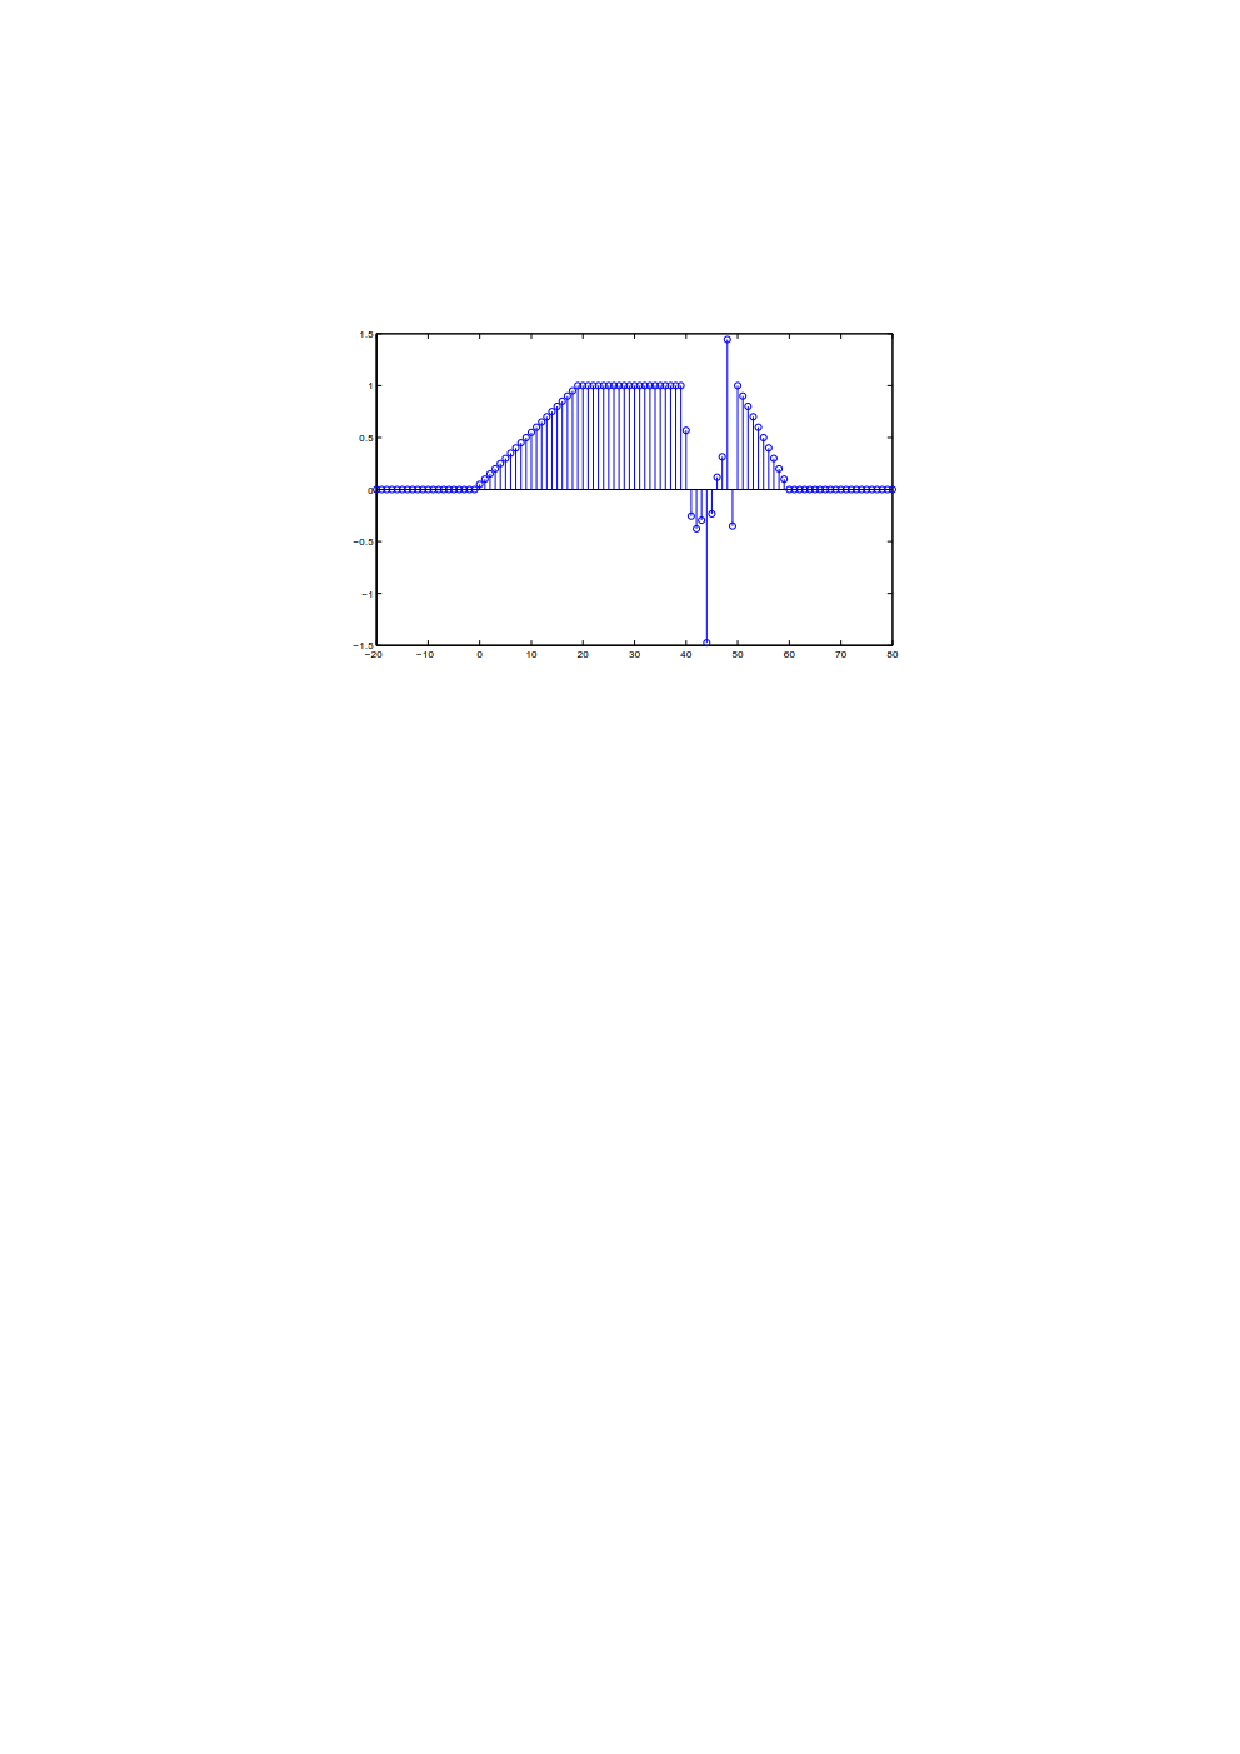
\includegraphics[width=0.6\textwidth]{Figures/Figure2-1}\\
  \caption{Un signal  \`a support fini}\label{fig:figure2-1}
\end{figure}

\begin{figure}
  \centering
  % Requires \usepackage{graphicx}
  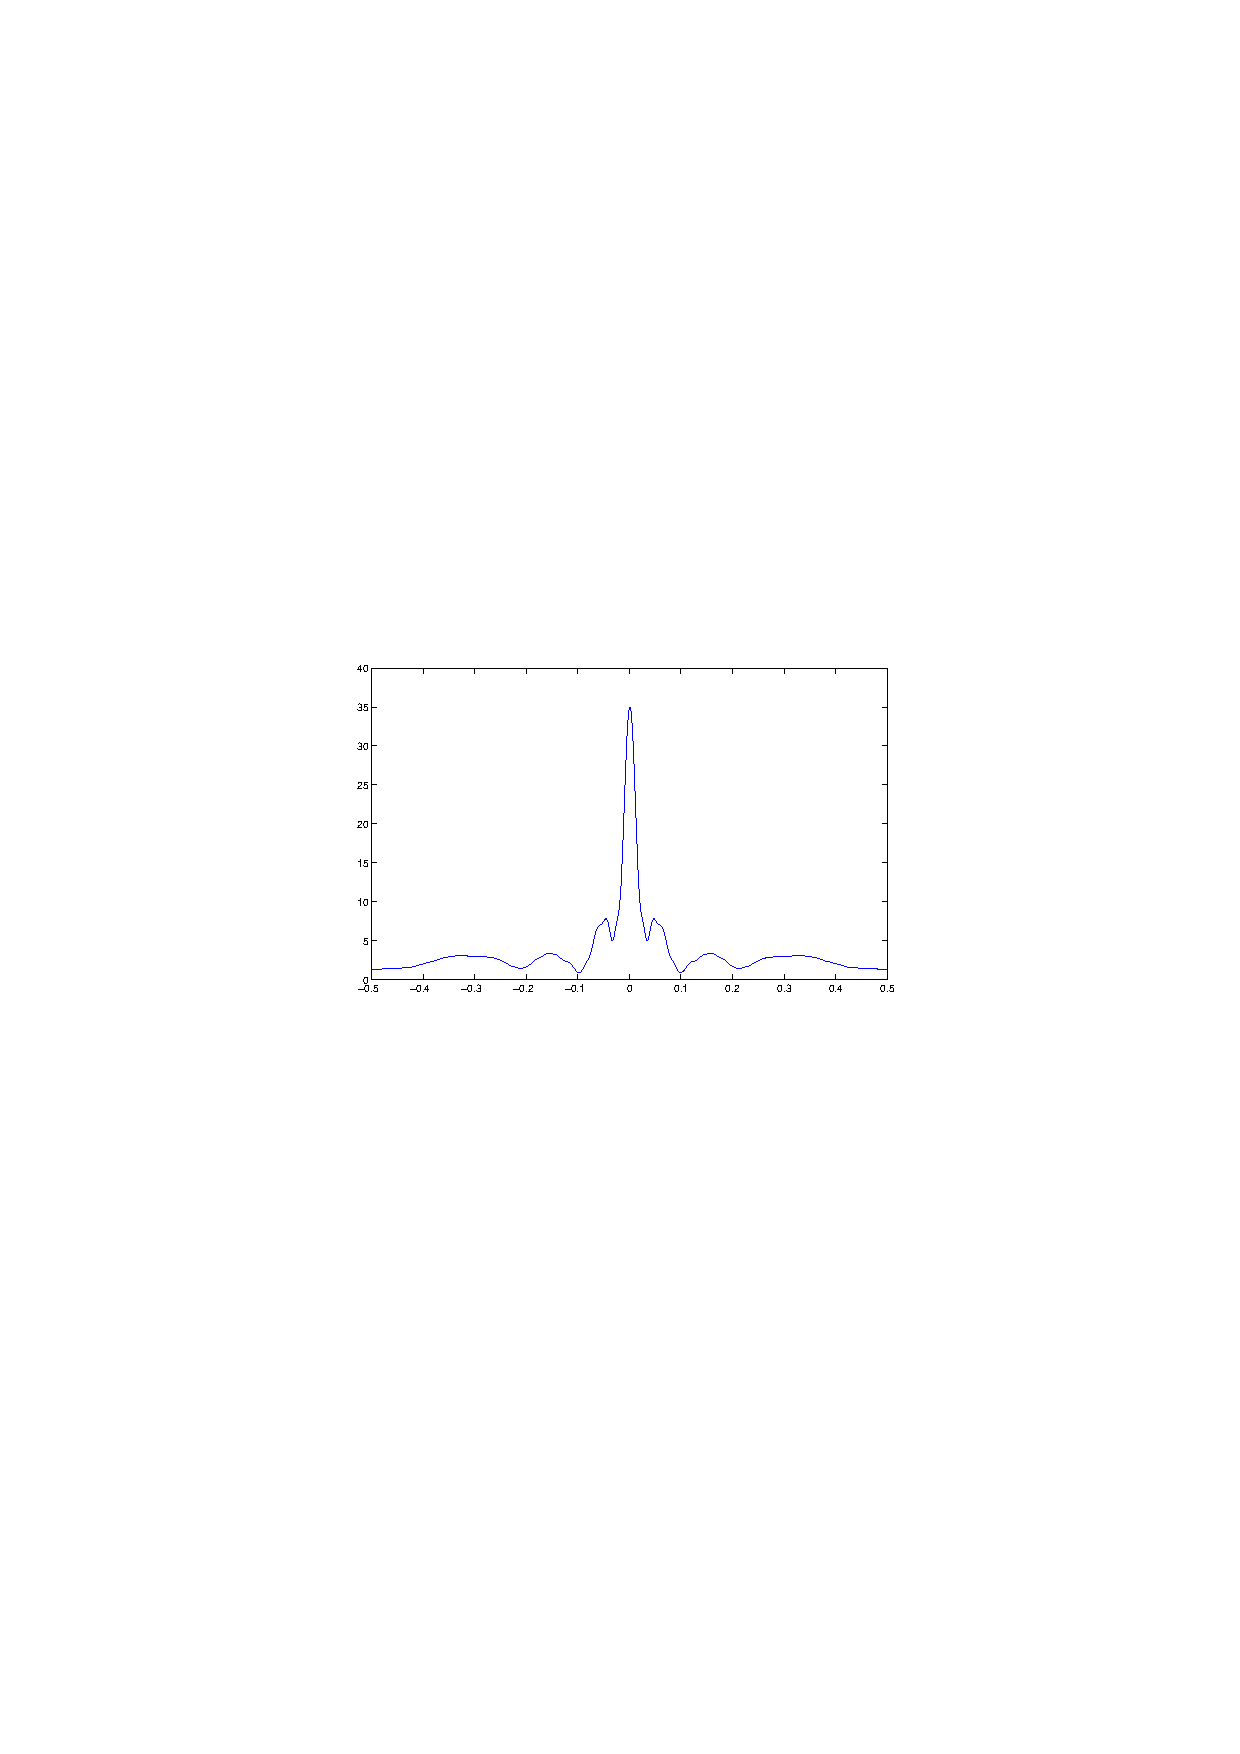
\includegraphics[width=0.6\textwidth]{Figures/Figure2-2}\\
  \caption{module de la TFtD du signal; comme le signal est r\'eel, le module de la TFtD est une fonction paire}\label{fig:figure2-2}
\end{figure}

\begin{figure}
  \centering
  % Requires \usepackage{graphicx}
  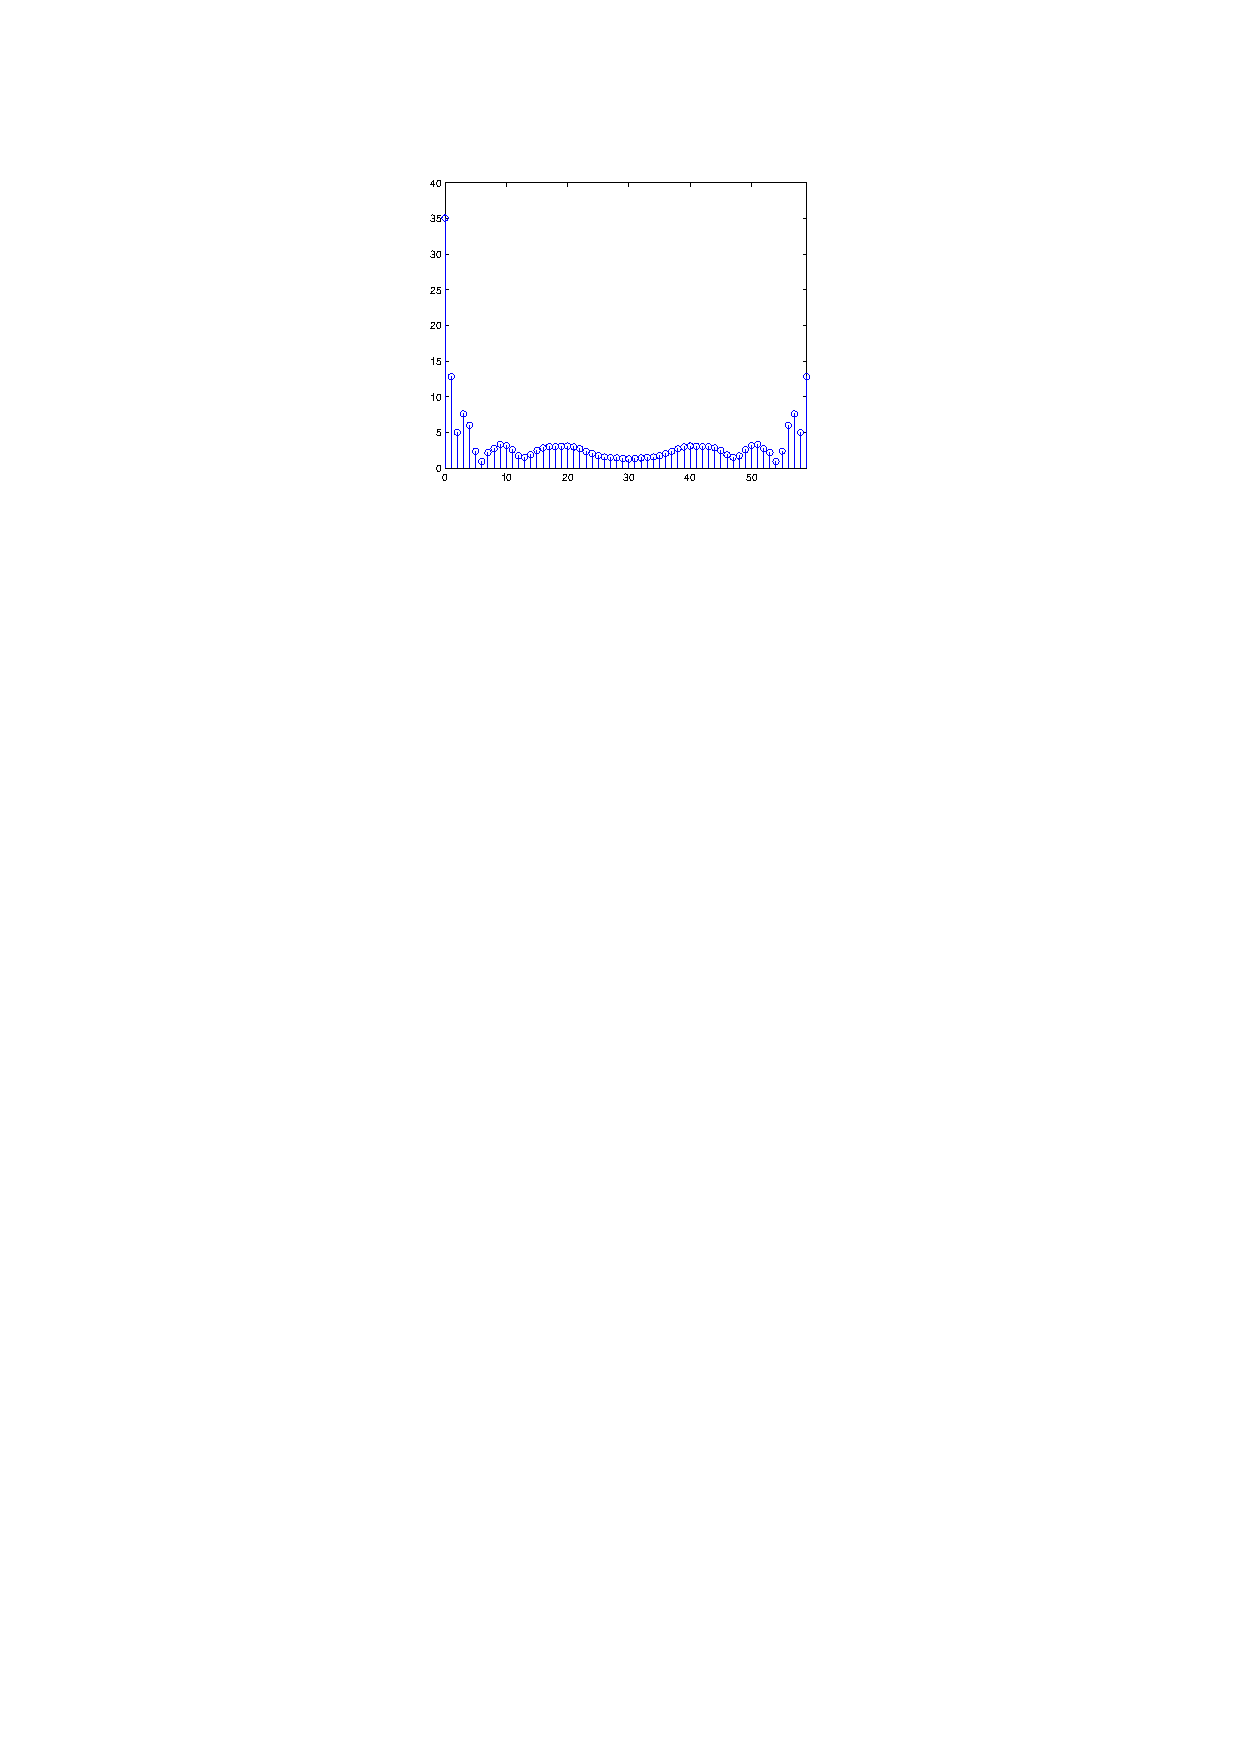
\includegraphics[width=0.6\textwidth]{Figures/Figure2-3}\\
  \caption{module de la TFD du signal}\label{fig:figure2-3}
\end{figure}

\begin{figure}
  \centering
  % Requires \usepackage{graphicx}
  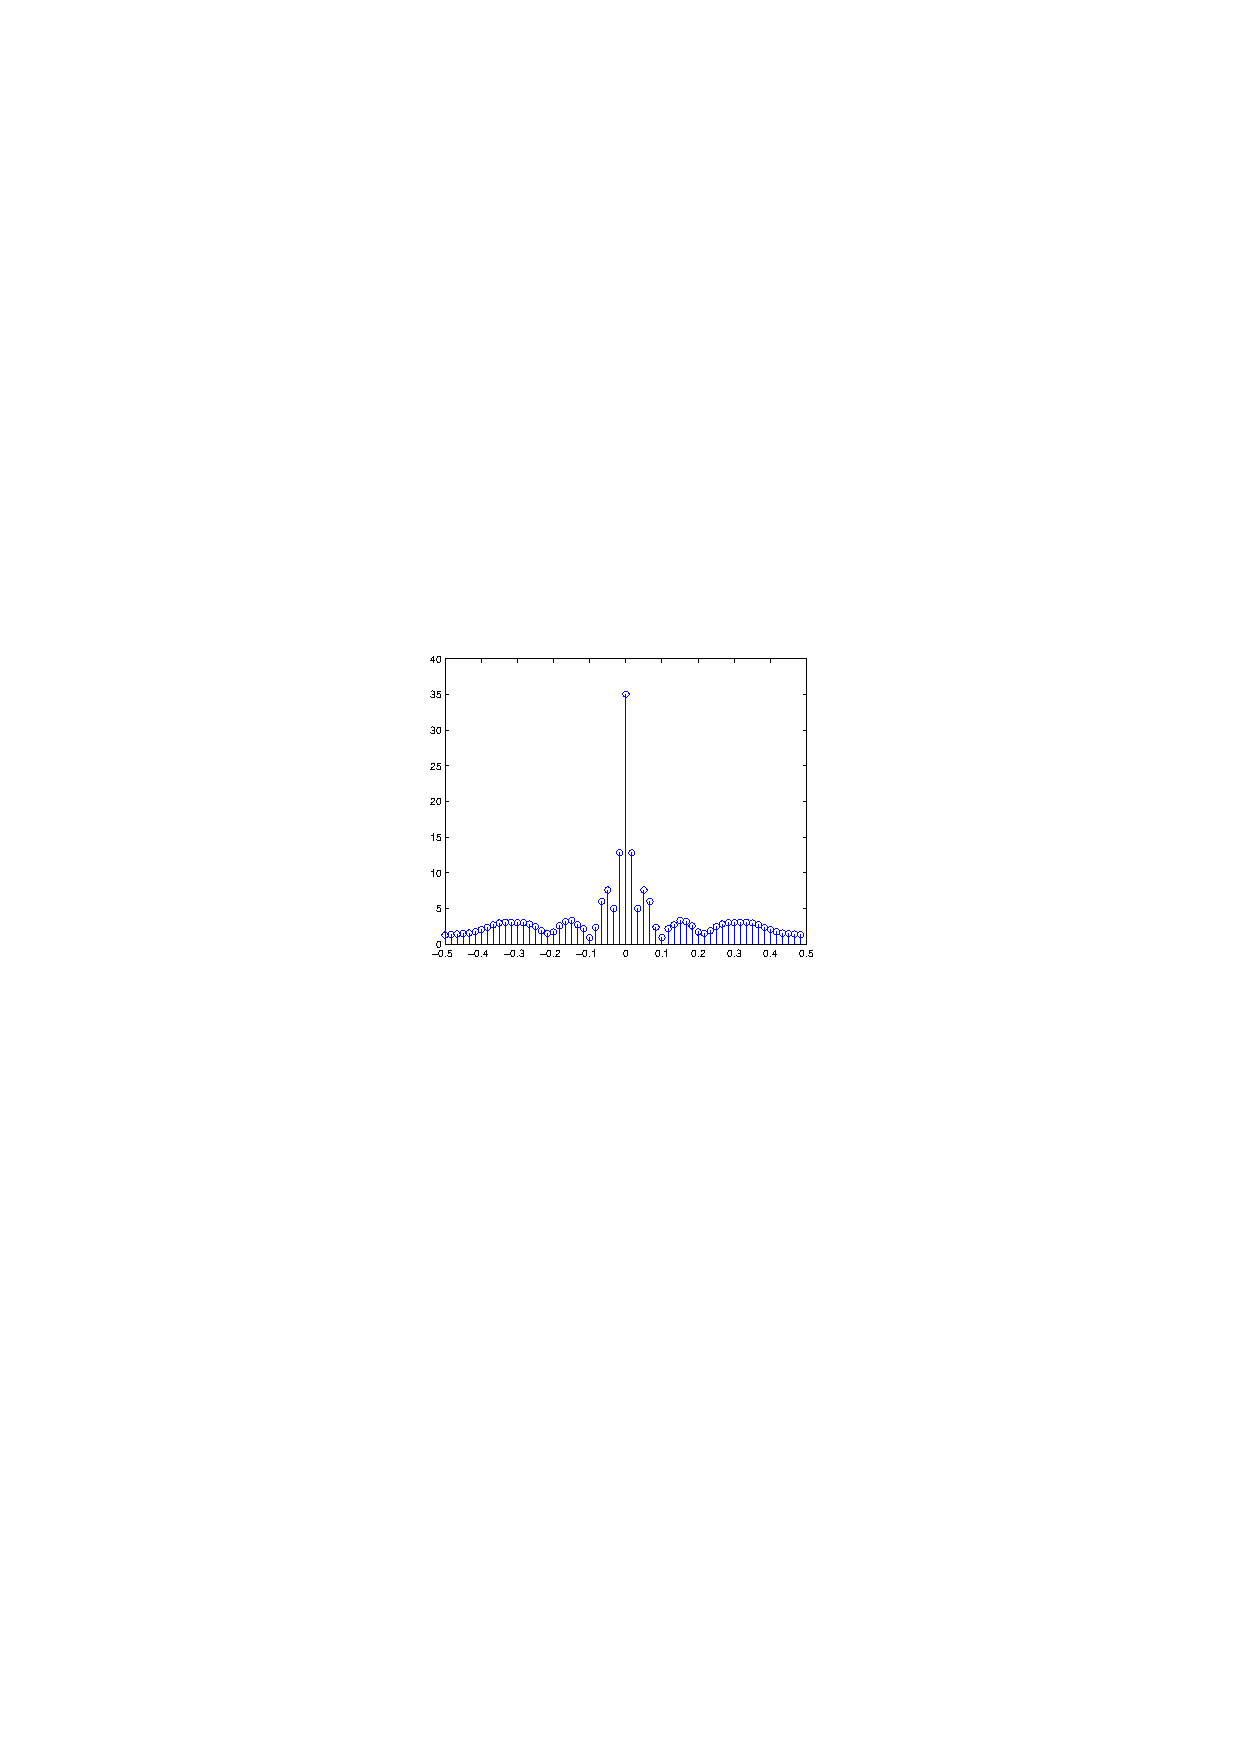
\includegraphics[width=0.6\textwidth]{Figures/Figure2-4}\\
  \caption{module de la TFD p\'eriodis\'e et remise \`a l'\'echelle}\label{fig:figure2-4}
\end{figure}

\subsubsection{Estimation d'une fr\'equence}
Soit $u_{n}=e^{2i\pi 1/0n}$ On voudrait d\'{e}terminer la fr\'{e}quence $\nu_{0}$ en ne se donnant le droit que d'observer les \'{e}chantillons $u_{0}, \ldots, u_{N}$. Pourquoi une telle contrainte? Dans un signal, musical par exemple, le contenu fr\'{e}quentiel \'{e}volue au cours du temps. \`{A} chaque changement de note, le signal contient sinusoïdes de fr\'{e}quences diff\'{e}rentes. Si l'on veut, par exemple, transcrire un morceau de musique en notes, on ne peut pas se permettre une observation sur une trop longue p\'{e}riode car cela aurait pour effet de m\'{e}langer entre elles diff\'{e}rentes notes. La m\^{e}me chose vaut pour l'analyse d'un signal de parole o\`{u} l'on risque la confusion entre diff\'{e}rents phon\`{e}mes.

On note $u^{T}$ la suite d\'{e}finie sur $\zset$ \'{e}gale \`{a} $u$ sur $\{0,\ \ldots,\ N-1\}$ et nulle ailleurs. Ce sont les seules valeurs que nous nous donnons le droit d'utiliser pour d\'{e}terminer $\nu_{0}$. Sa TFtD est donnée pour tout
$\nu\in \coint{1/2,1/2}$ par
$$
\TFA{u^{T}}(\nu)=\rme^{-\rmi \pi (N-1)(\nu- \nu_0)} \frac{\sin(N\pi(\nu-\nu_{0}))}{sin(\pi(\nu-\nu_{0}))}
$$
La \Cref{fig:figure2-6} représente le module de $\mathcal{F}(u^{T})$.
\begin{figure}
  \centering
  % Requires \usepackage{graphicx}
  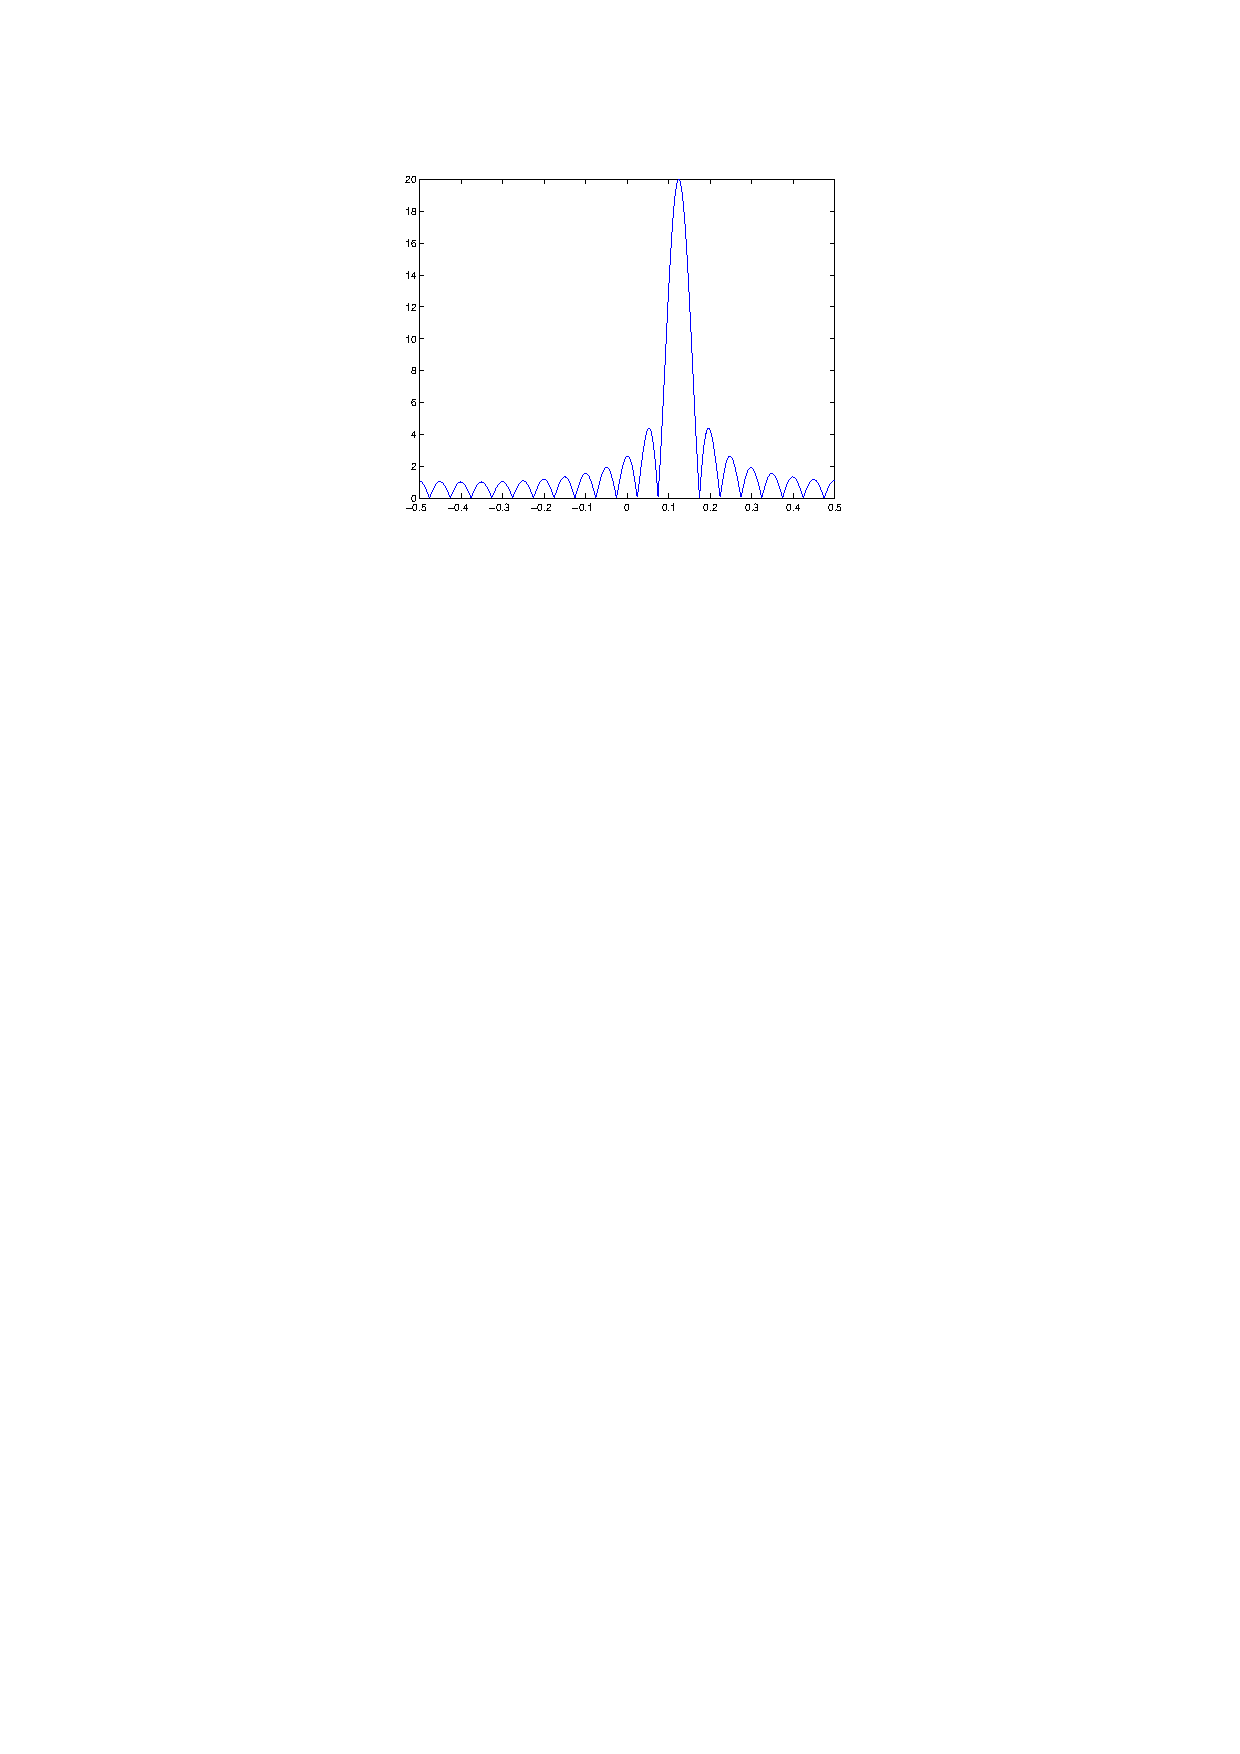
\includegraphics[width=0.6\textwidth]{Figures/Figure2-6}\\
  \caption{La TFD d'ordre 30 de l'harmonique complexe tronqu\'{e}e superpos\'{e}e \`{a} la TFtD. Le maximum de la TFD est atteint pour $k=4$, soit une fr\'{e}quence de $4/30=0$, 1333 et une erreur d'estimation de 0,01}\label{fig:figure2-6}
\end{figure}


Si on calcule une TFD d'ordre $M\geq N$, on sait que l'on va \'{e}chantillonner la TFtD de $u^{T}$ aux point $k/M$. Deux TFD d'ordres diff\'{e}rents sont donn\'{e}es \Cref{fig:figure2-7} et \Cref{fig:figure2-8}.


Avec une $TFD$ d'ordre $M$ on peut estimer la fr\'{e}quence de l'harmonique complexe $\nu_{0}$ avec une pr\'{e}cision d'au moins $1/M$.
En effet, quelque soit $\nu_{0} \in \coint{-1/2,1/2}$ il existe au moins un $k$ tel que  $|k/M - \nu_0| \leq 1/M$.
\begin{figure}
  \centering
  % Requires \usepackage{graphicx}
  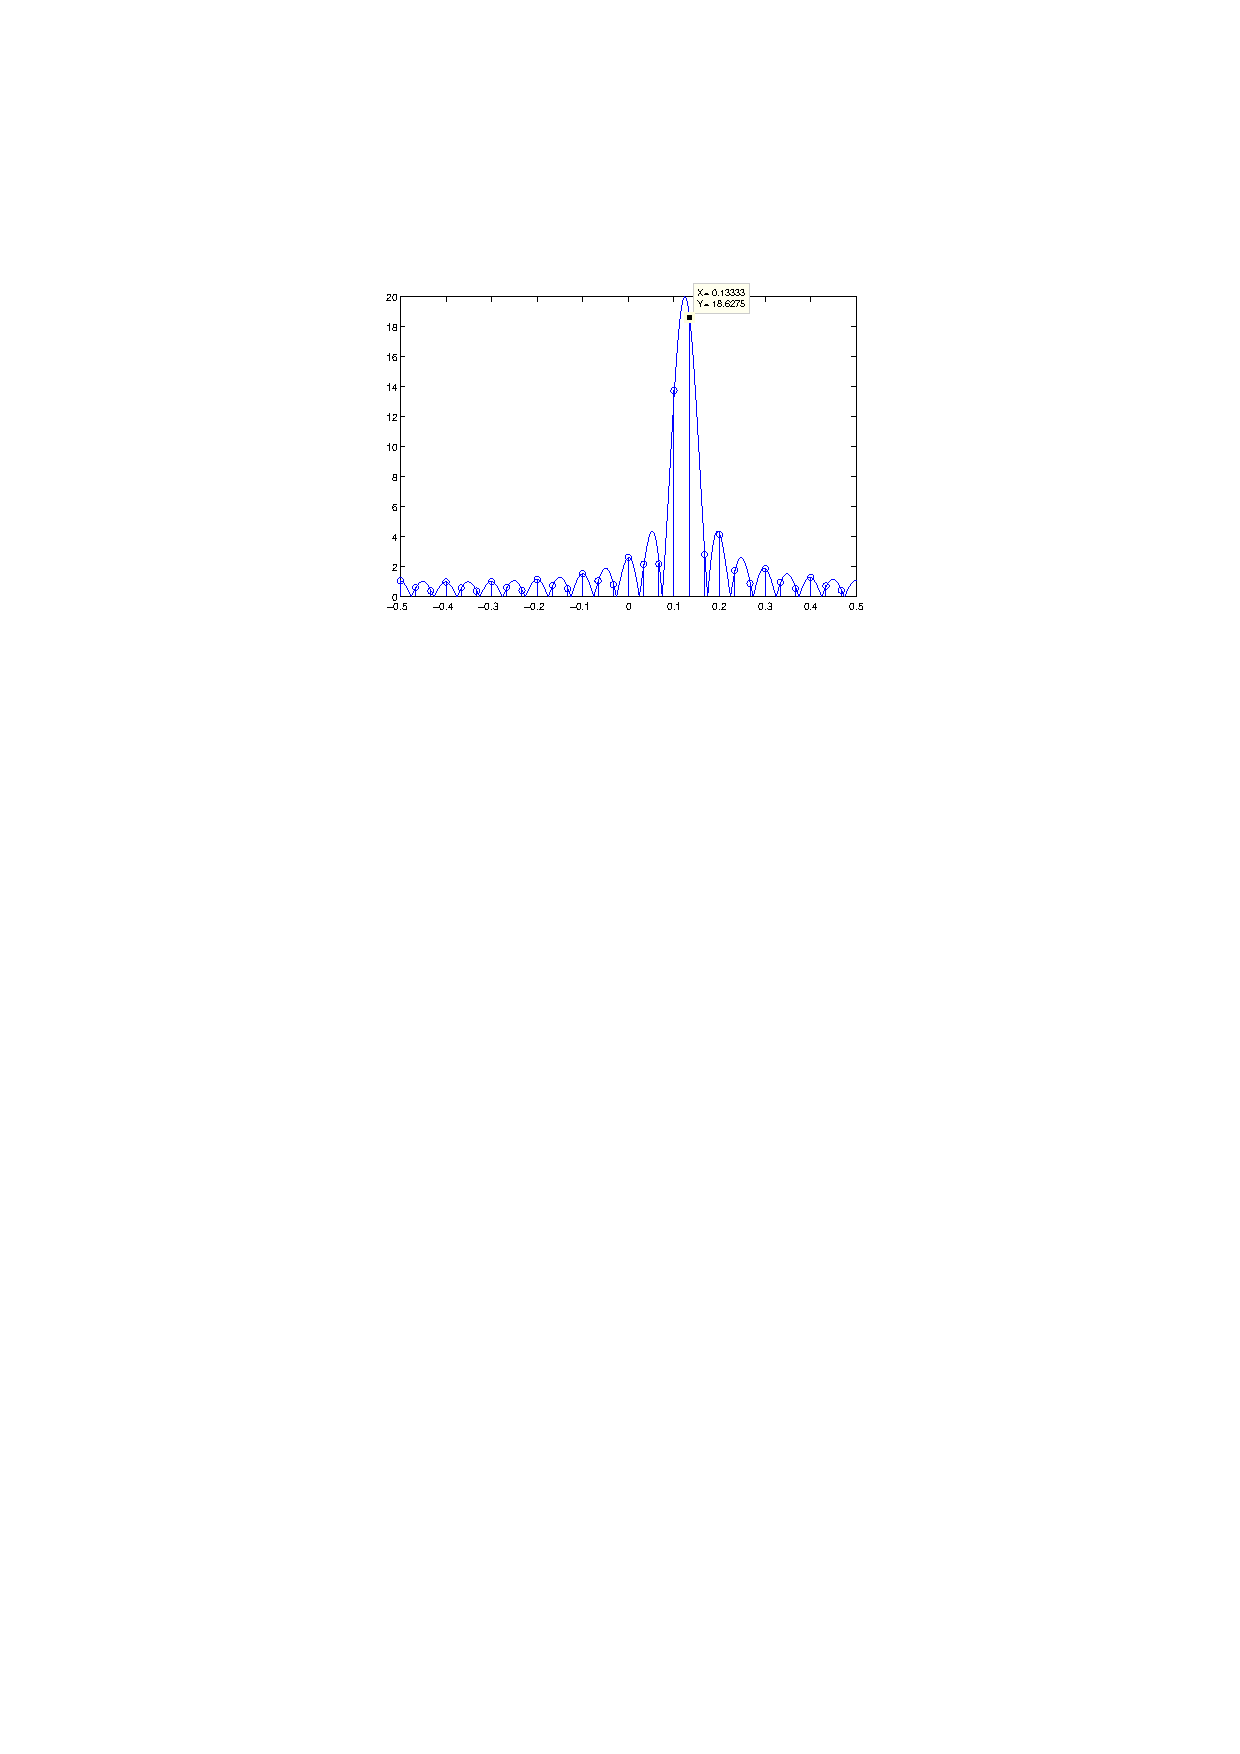
\includegraphics[width=0.6\textwidth]{Figures/Figure2-7}\\
  \caption{La TFD d'ordre 30 de l'harmonique complexe tronqu\'{e}e superpos\'{e}e \`{a} la TFtD. Le maximum de la TFD est atteint pour $k=4$, soit une fr\'{e}quence de $4/30=0$, 1333 et une erreur d'estimation de 0,01}\label{fig:figure2-7}
\end{figure}


\begin{figure}
  \centering
  % Requires \usepackage{graphicx}
  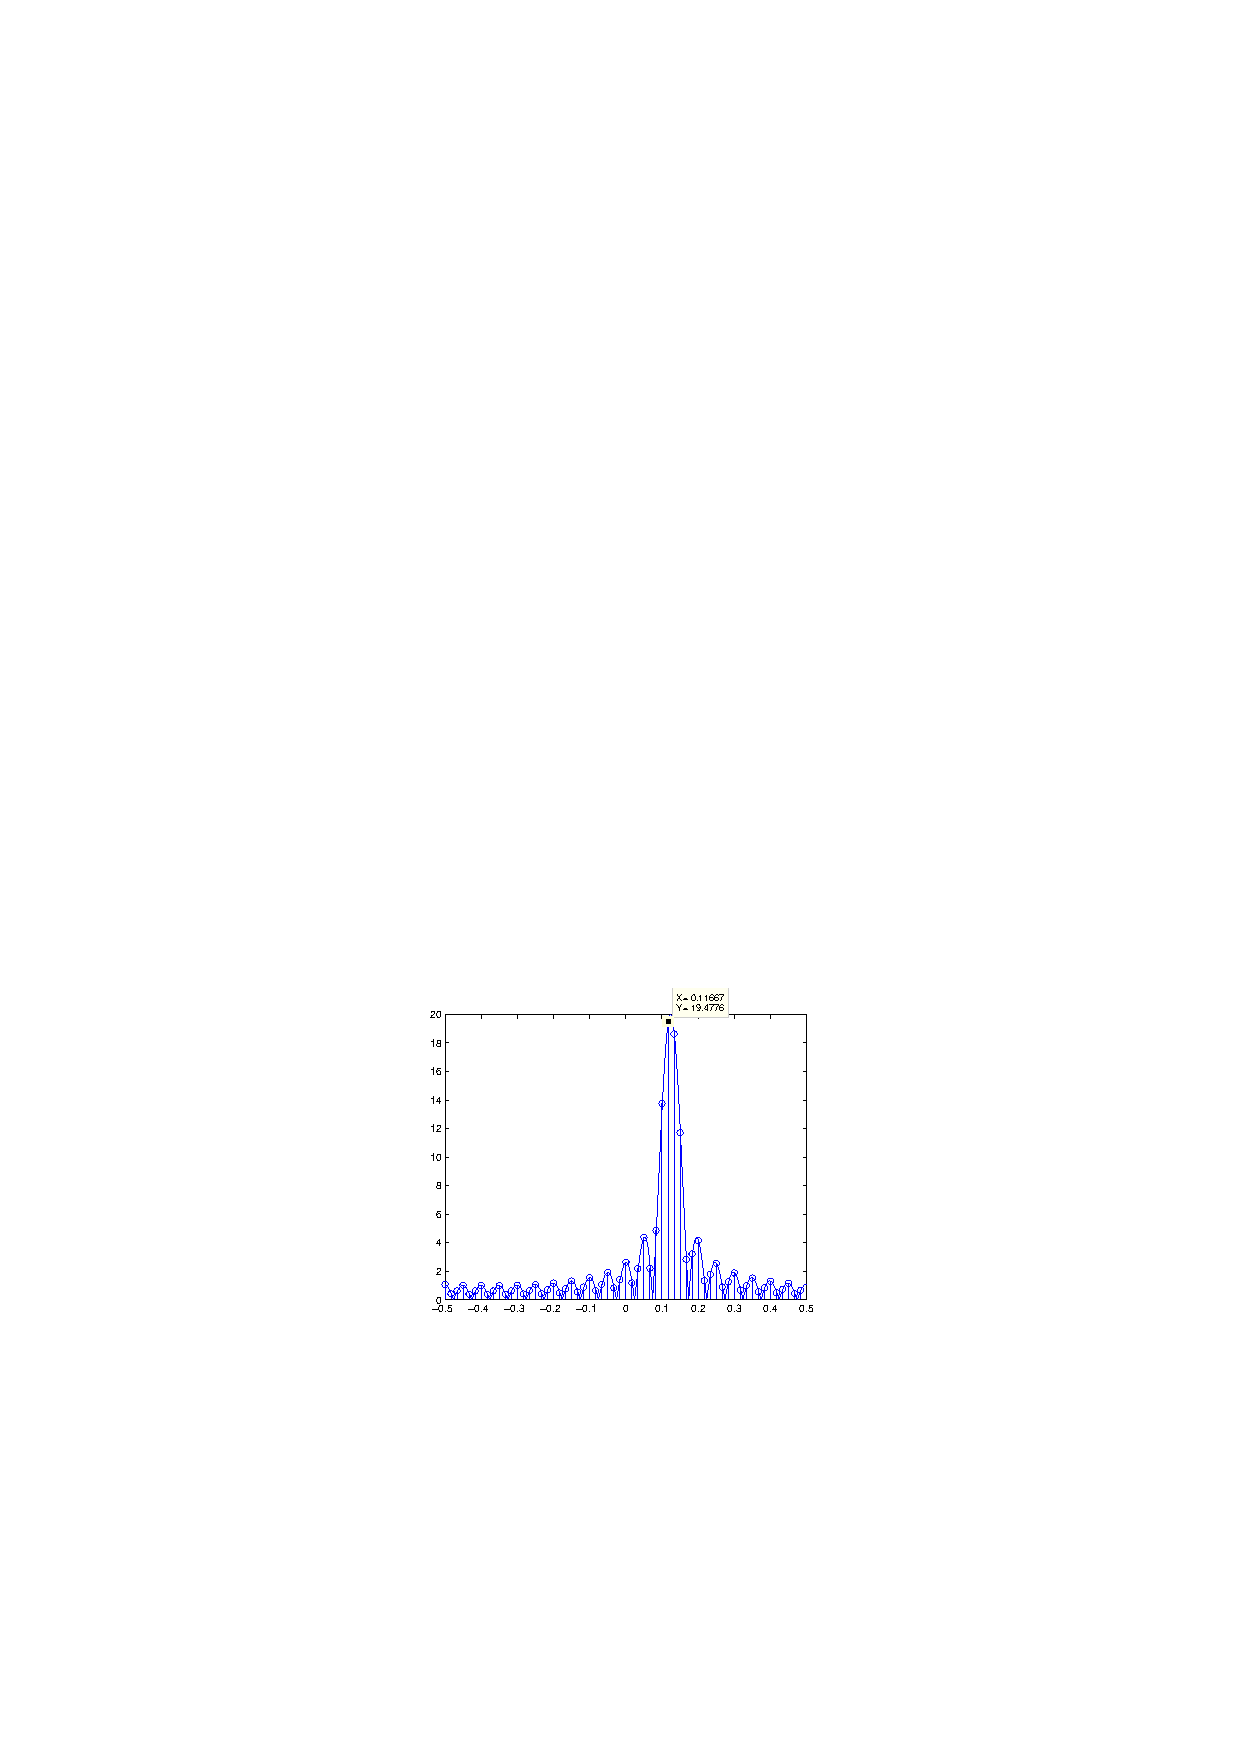
\includegraphics[width=0.6\textwidth]{Figures/Figure2-8}\\
  \caption{La TFD d'ordre 60 de l'harmonique complexe tronqu\'{e}e superpos\'{e}e \`{a} la TFtD. Le maximum de la TFD est atteint pour $k=7$, soit une fr\'{e}quence de $7/60=0$, 11667 et une erreur d'estimation de 0,0063}\label{fig:figure2-8}
\end{figure}




\subsection{S\'{e}paration de deux exponentielles complexes et fen\^{e}trage}
Cette fois-ci on poss\`{e}de un signal plus complexe qui est la somme de deux harmoniques complexes sur $\zset$
$$
u_{n}=A_{0}\rme^{2\rmi\pi\nu_{0}n}+A_{1}\rme^{2\rmi\pi\nu_{1}n}
$$
Les inconnues ici, sont les amplitudes $A_{0}$ et $A_{1}$ ainsi que les fr\'{e}quences $\nu_{0}$ et $\nu_{1}$. Encore une fois on ne se donne le droit que d'observer $N$ \'{e}chantillons, et on note $u^{T}$ la suite ainsi tronqu\'{e}e.


Les graphiques de \Cref{fig:figure2-9} \`{a} \Cref{fig:figure2-12} illustrent le probl\`{e}me de la r\'{e}solution fr\'{e}quentielle en calculant la TFtD de $u^{T}$ pour diff\'{e}rentes valeurs de $N$.

On constate qu'il faut au moins avoir $|\nu_{0}-\nu_{1}|>1/N$ pour pouvoir distinguer deux pics sur la TFtD. Sinon, les deux pics se confondent en un seul et il sera impossible de distinguer $\nu_{0}$ et $\nu_{1}.$

\begin{figure}
  \centering
  % Requires \usepackage{graphicx}
  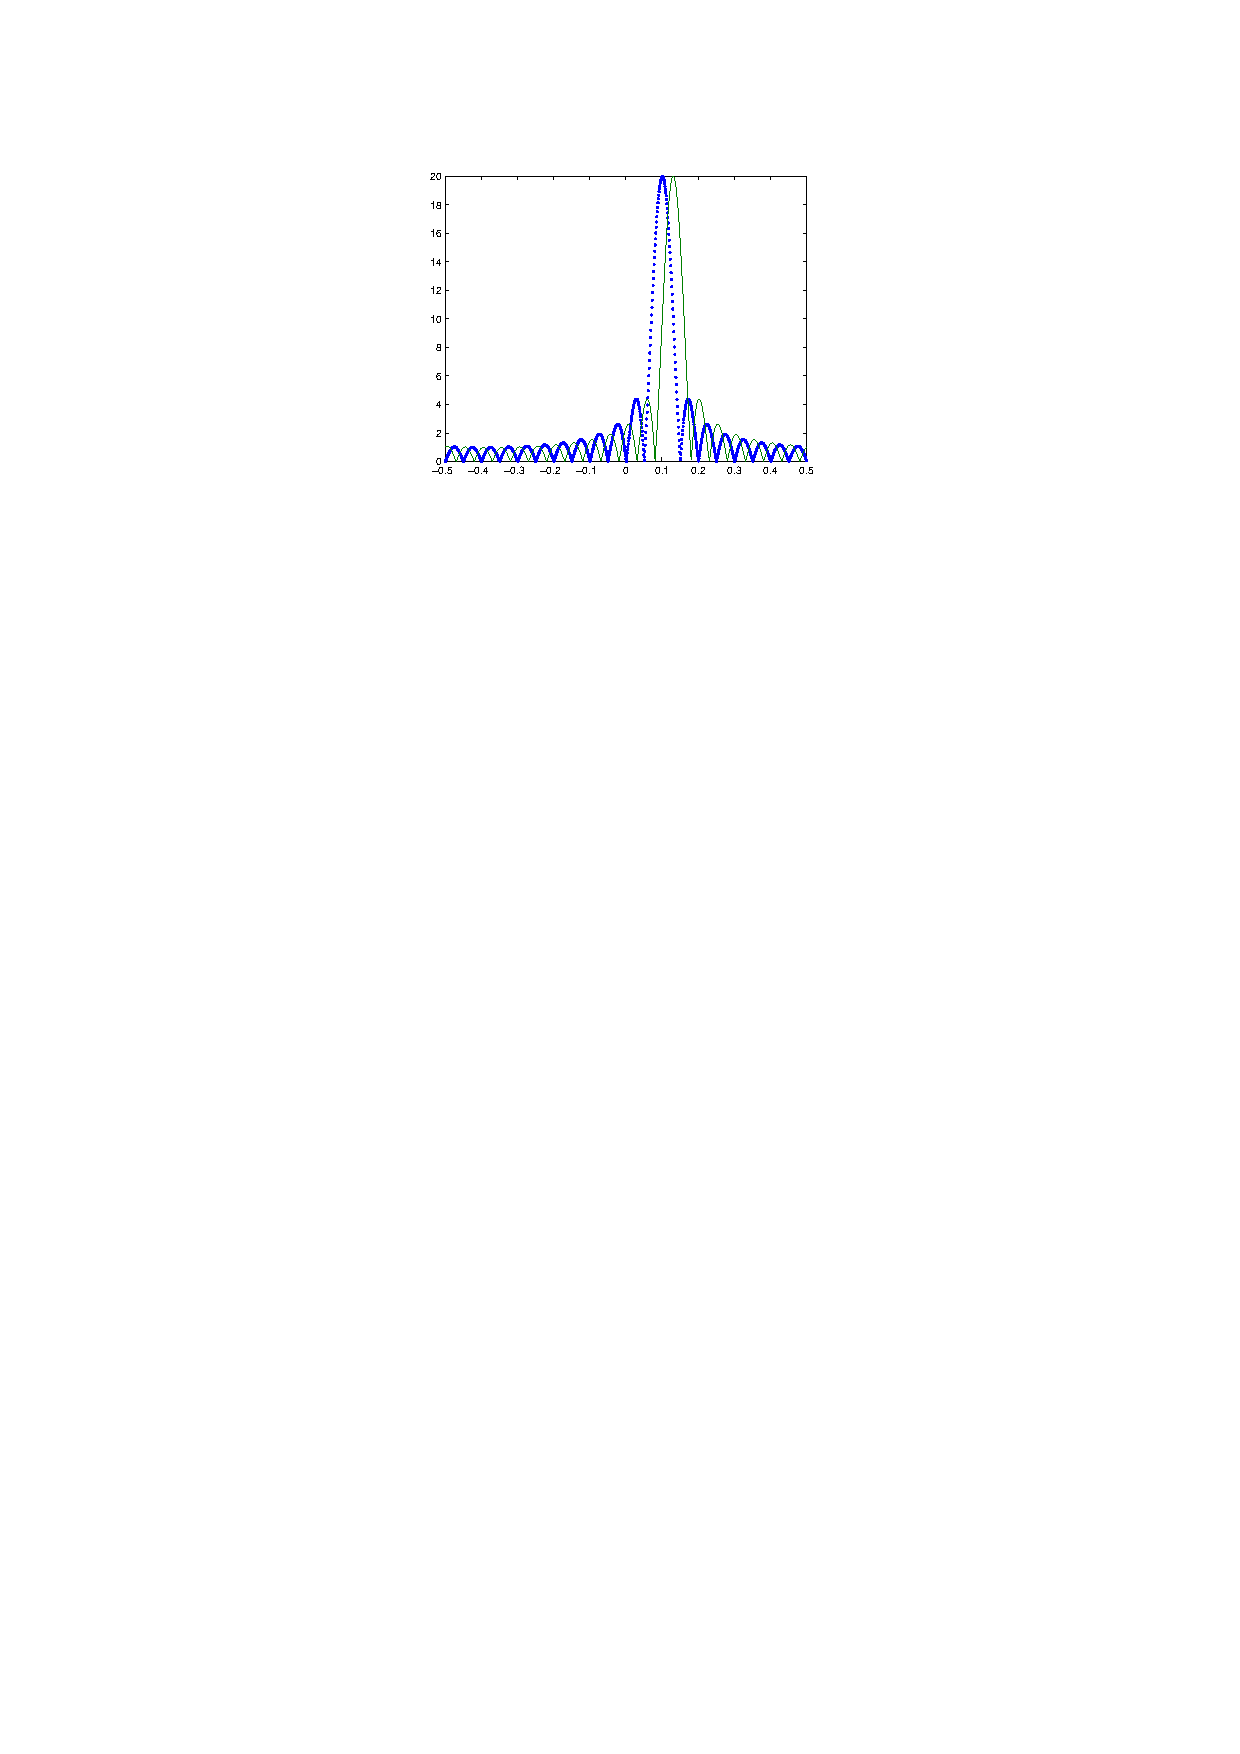
\includegraphics[width=0.6\textwidth]{Figures/Figure2-9}\\
  \caption{On a utilis\'{e} seulement $N=20$ \'{e}chantillons pour tracer la TFtD de deux ondes (l'une en pointill\'{e}s, l'autre en trait plein) de m\^{e}me module et de fr\'{e}quences 0,1 et 0,13.}\label{fig:figure2-9}
\end{figure}

\begin{figure}
  \centering
  % Requires \usepackage{graphicx}
  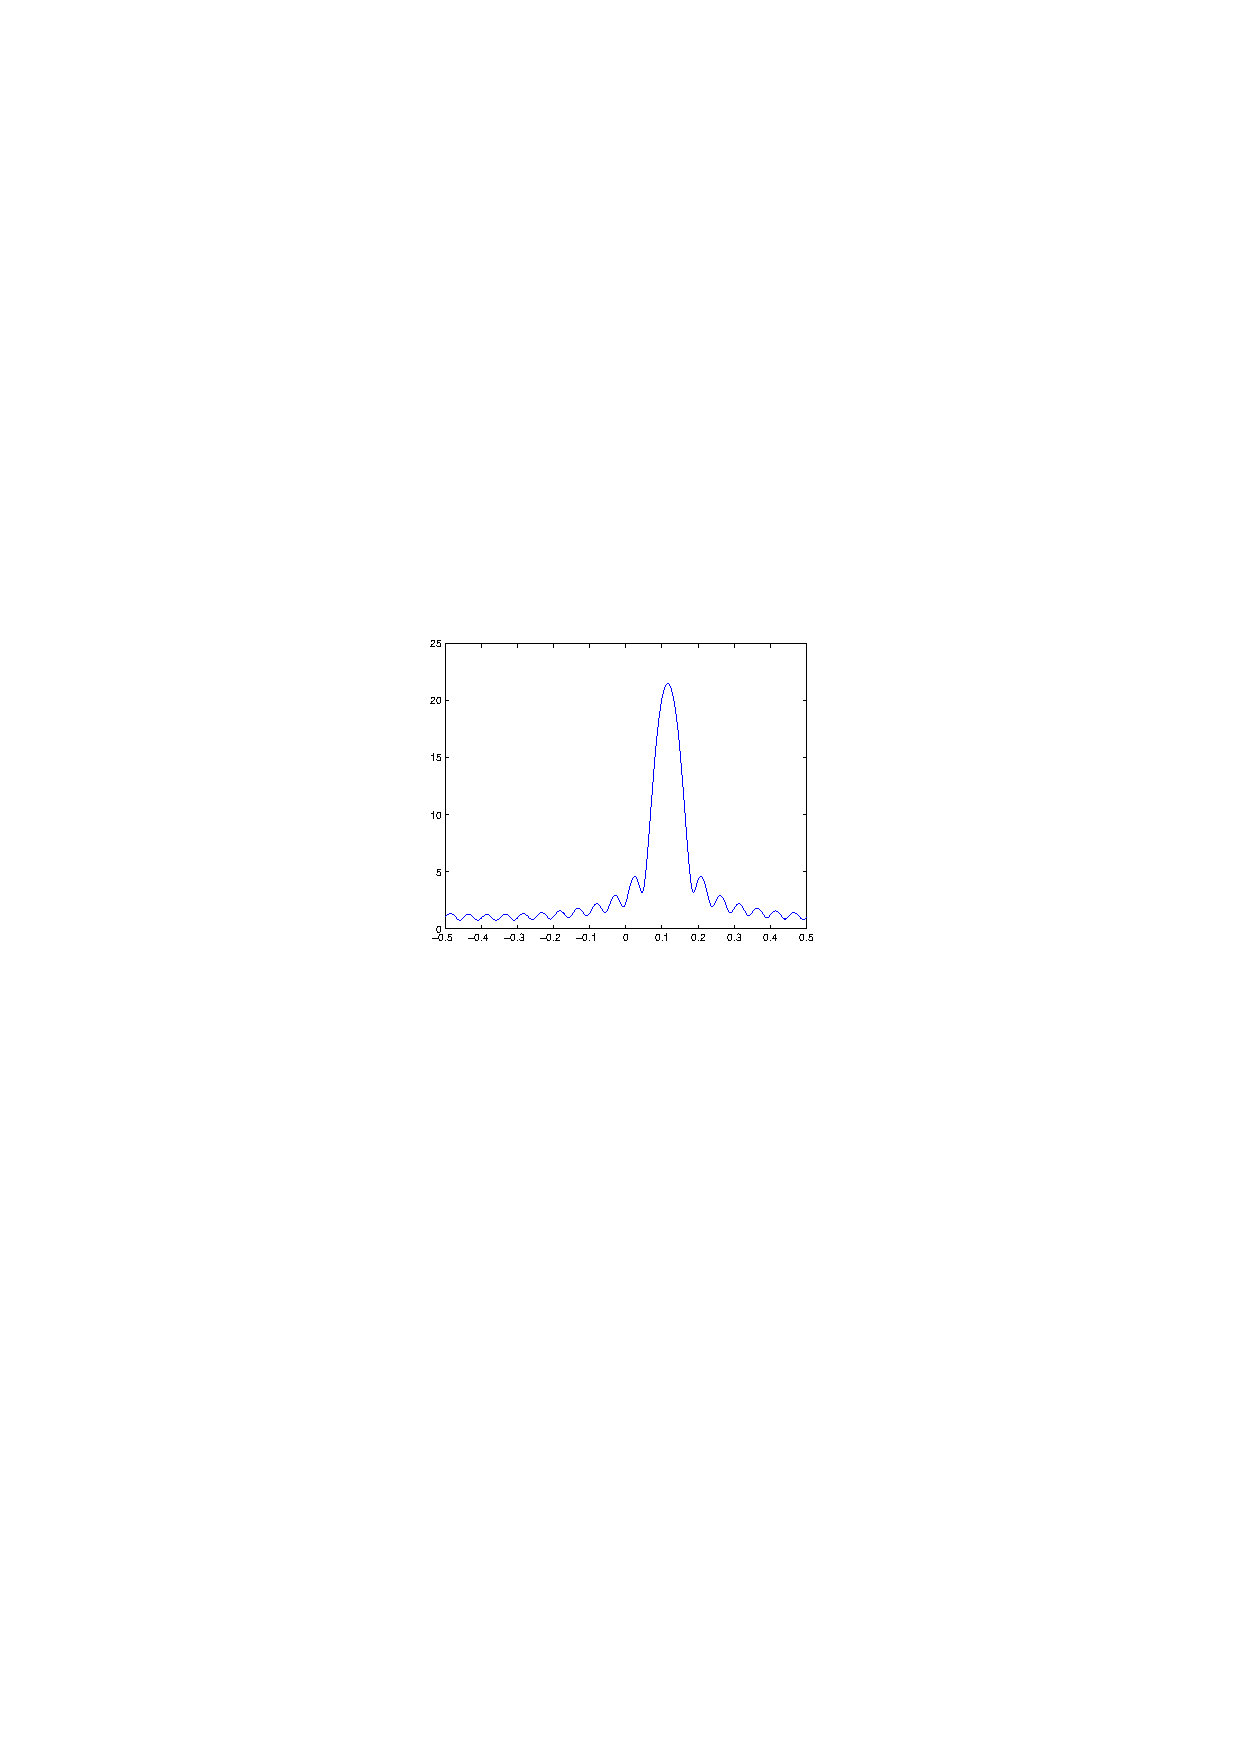
\includegraphics[width=0.6\textwidth]{Figures/Figure2-10}\\
  \caption{TFtD de la somme des deux ondes tronqu\'{e}es \`{a} 30 \'{e}chantillons (\Cref{fig:figure2-9}). On ne peut pas distinguer la superposition des deux harmoniques complexes dans le signal.}\label{fig:figure2-10}
\end{figure}

\begin{figure}
  \centering
  % Requires \usepackage{graphicx}
  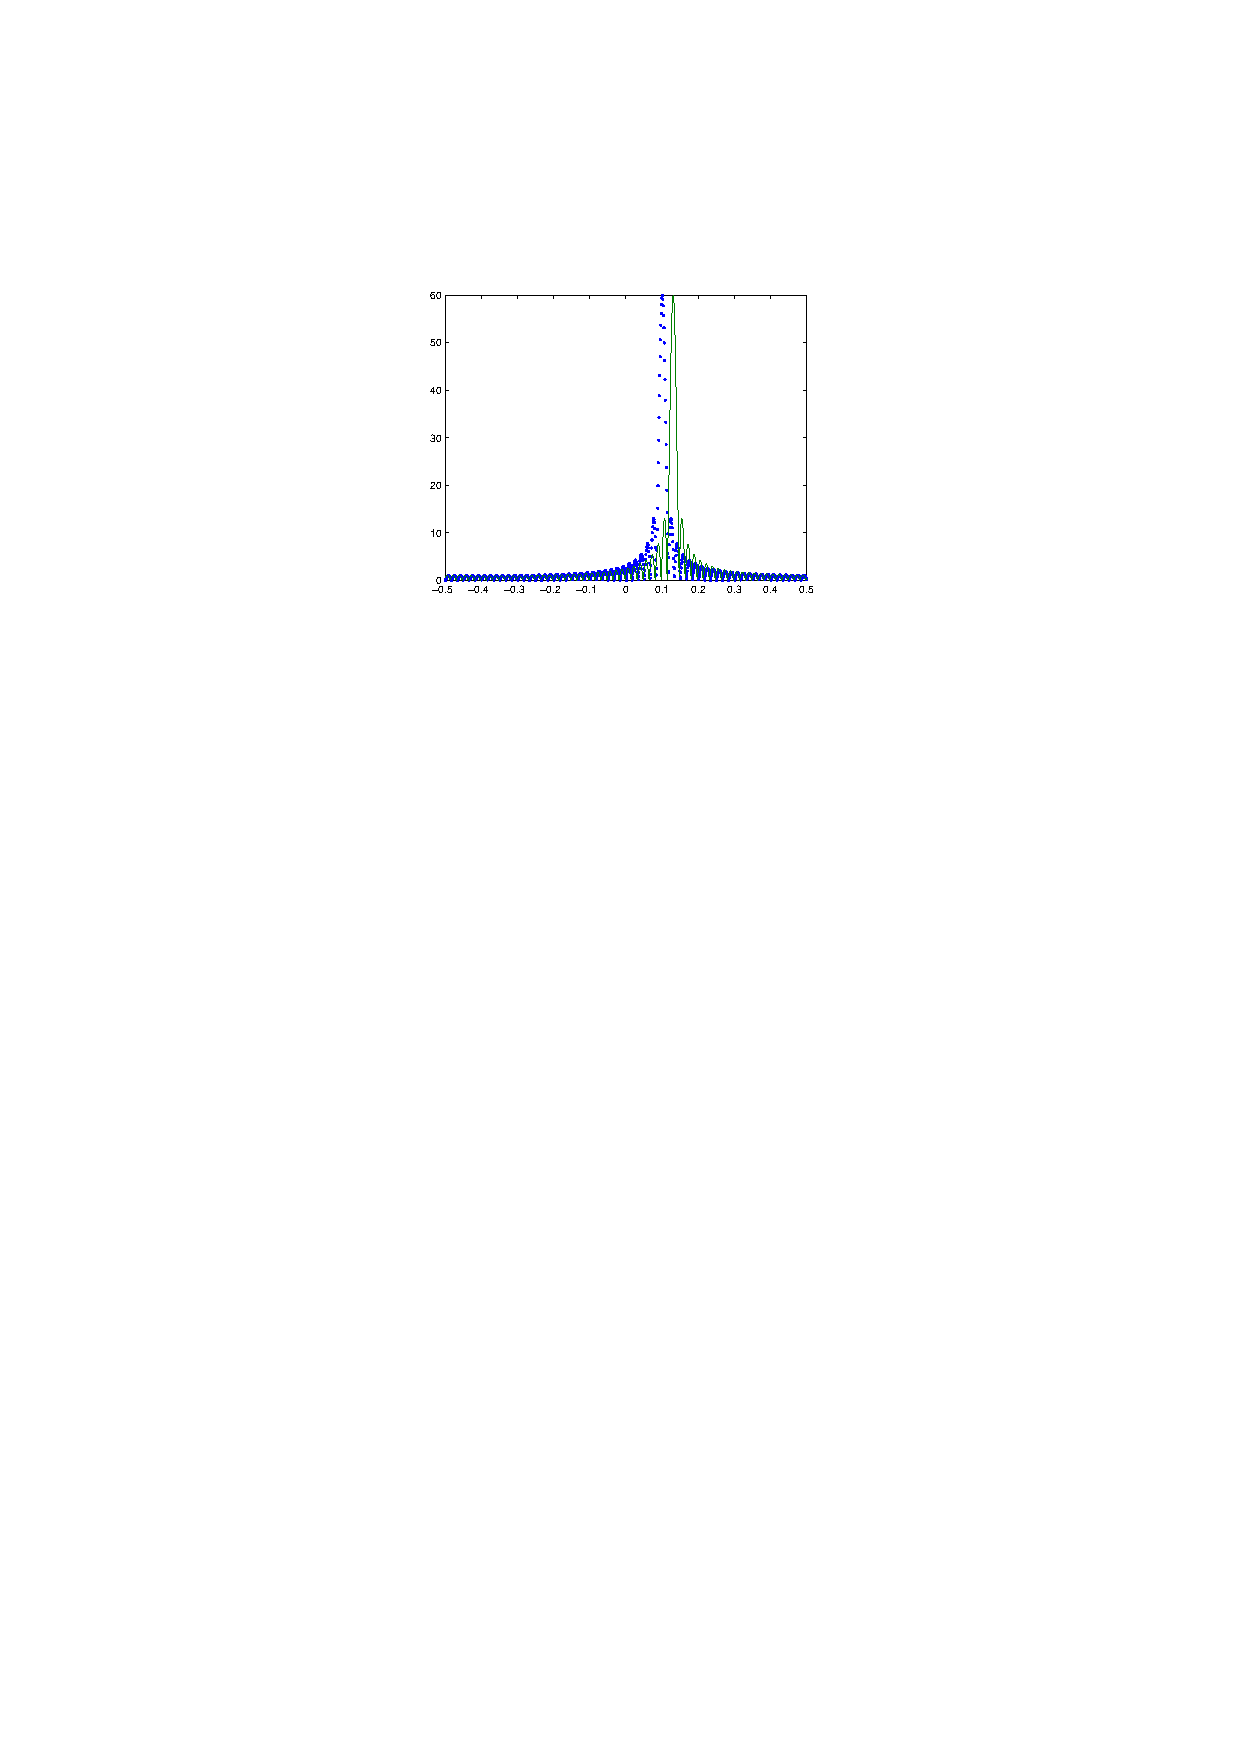
\includegraphics[width=0.6\textwidth]{Figures/Figure2-11}\\
  \caption{On a utilis\'{e} seulement $N=20$ \'{e}chantillons pour tracer la TFtD de deux ondes (l'une en pointill\'{e}s, l'autre en trait plein) de m\^{e}me module et de fr\'{e}quences 0,1 et 0,13.}\label{fig:figure2-11}
\end{figure}


\begin{figure}
  \centering
  % Requires \usepackage{graphicx}
  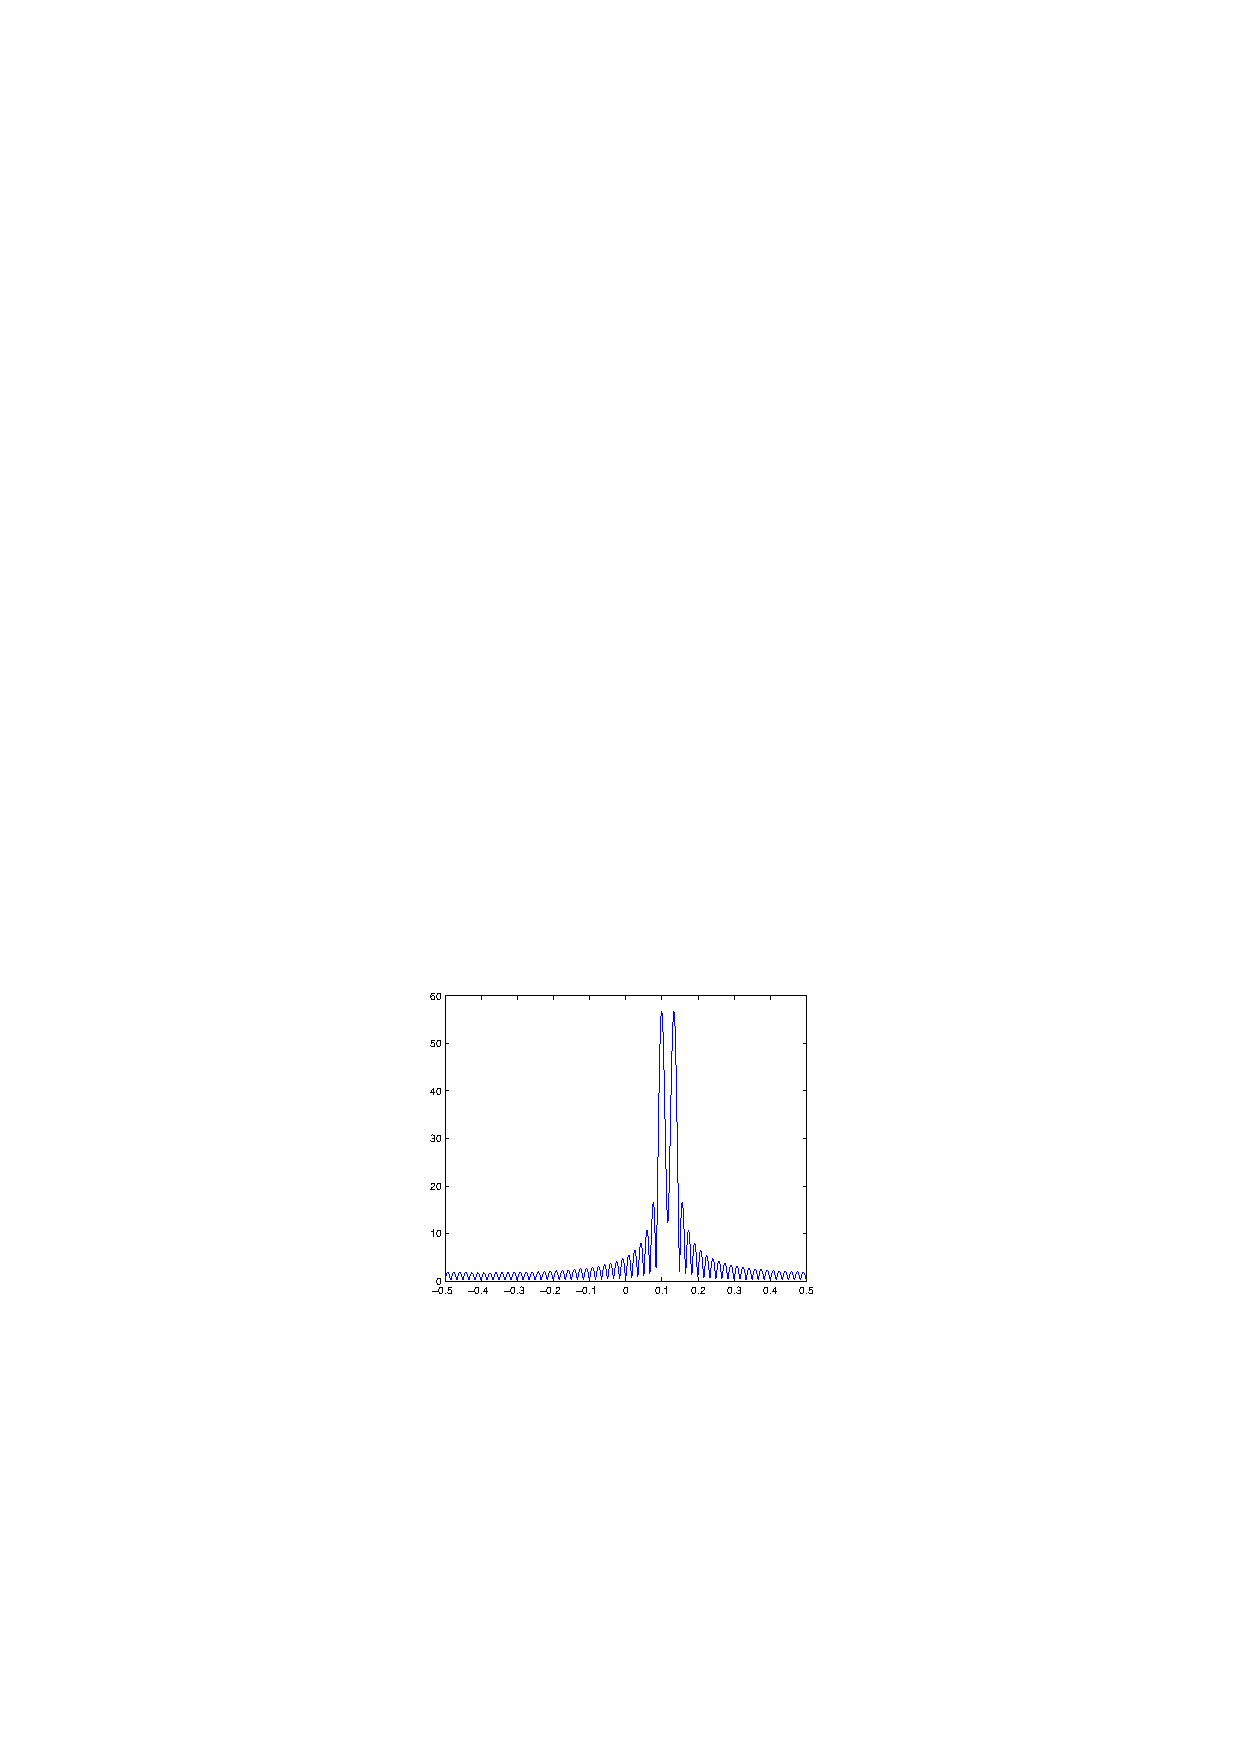
\includegraphics[width=0.6\textwidth]{Figures/Figure2-12}\\
  \caption{TFtD de la somme des deux ondes tronqu\'{e}es \`{a} 60 \'{e}chantillons (\Cref{fig:figure2-11}). Cette fois on distingue bien les deux ondes. Il a fallu prendre un nombre d'\'{e}chantillons $N$ sup\'{e}rieur \`{a} $1/(0.13-0.1)=33.3$ pour arriver \`{a} distinguer les deux.}\label{fig:figure2-12}
\end{figure}


\begin{figure}
  \centering
  % Requires \usepackage{graphicx}
  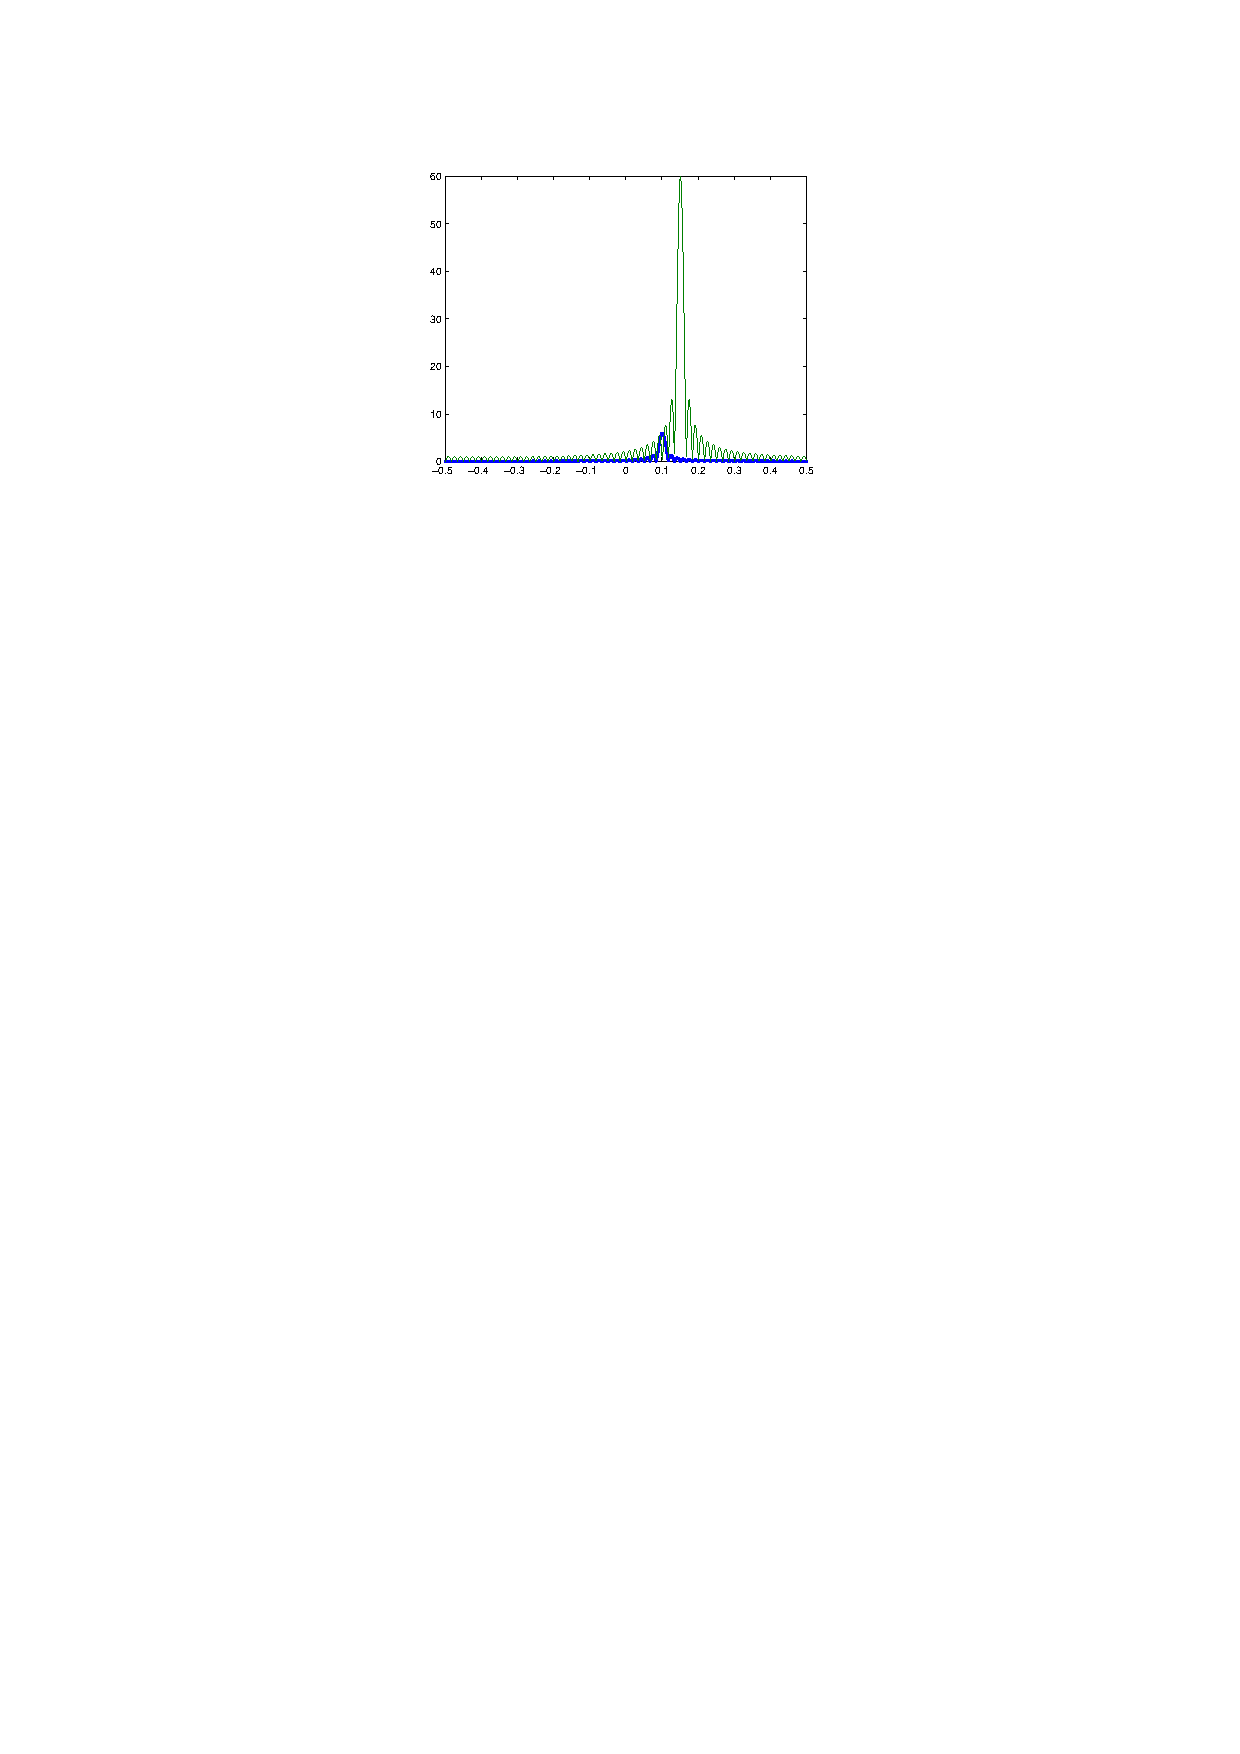
\includegraphics[width=0.6\textwidth]{Figures/Figure2-13}\\
  \caption{TFtD de deux ondes tronqu\'{e}es dont l'une a une amplitude 10 fois plus petite que l'autre. La plus petite des deux est cach\'{e}e par les lobes secondaires de la TFtD de l'autre.}\label{fig:figure2-13}
\end{figure}


\begin{figure}
  \centering
  % Requires \usepackage{graphicx}
  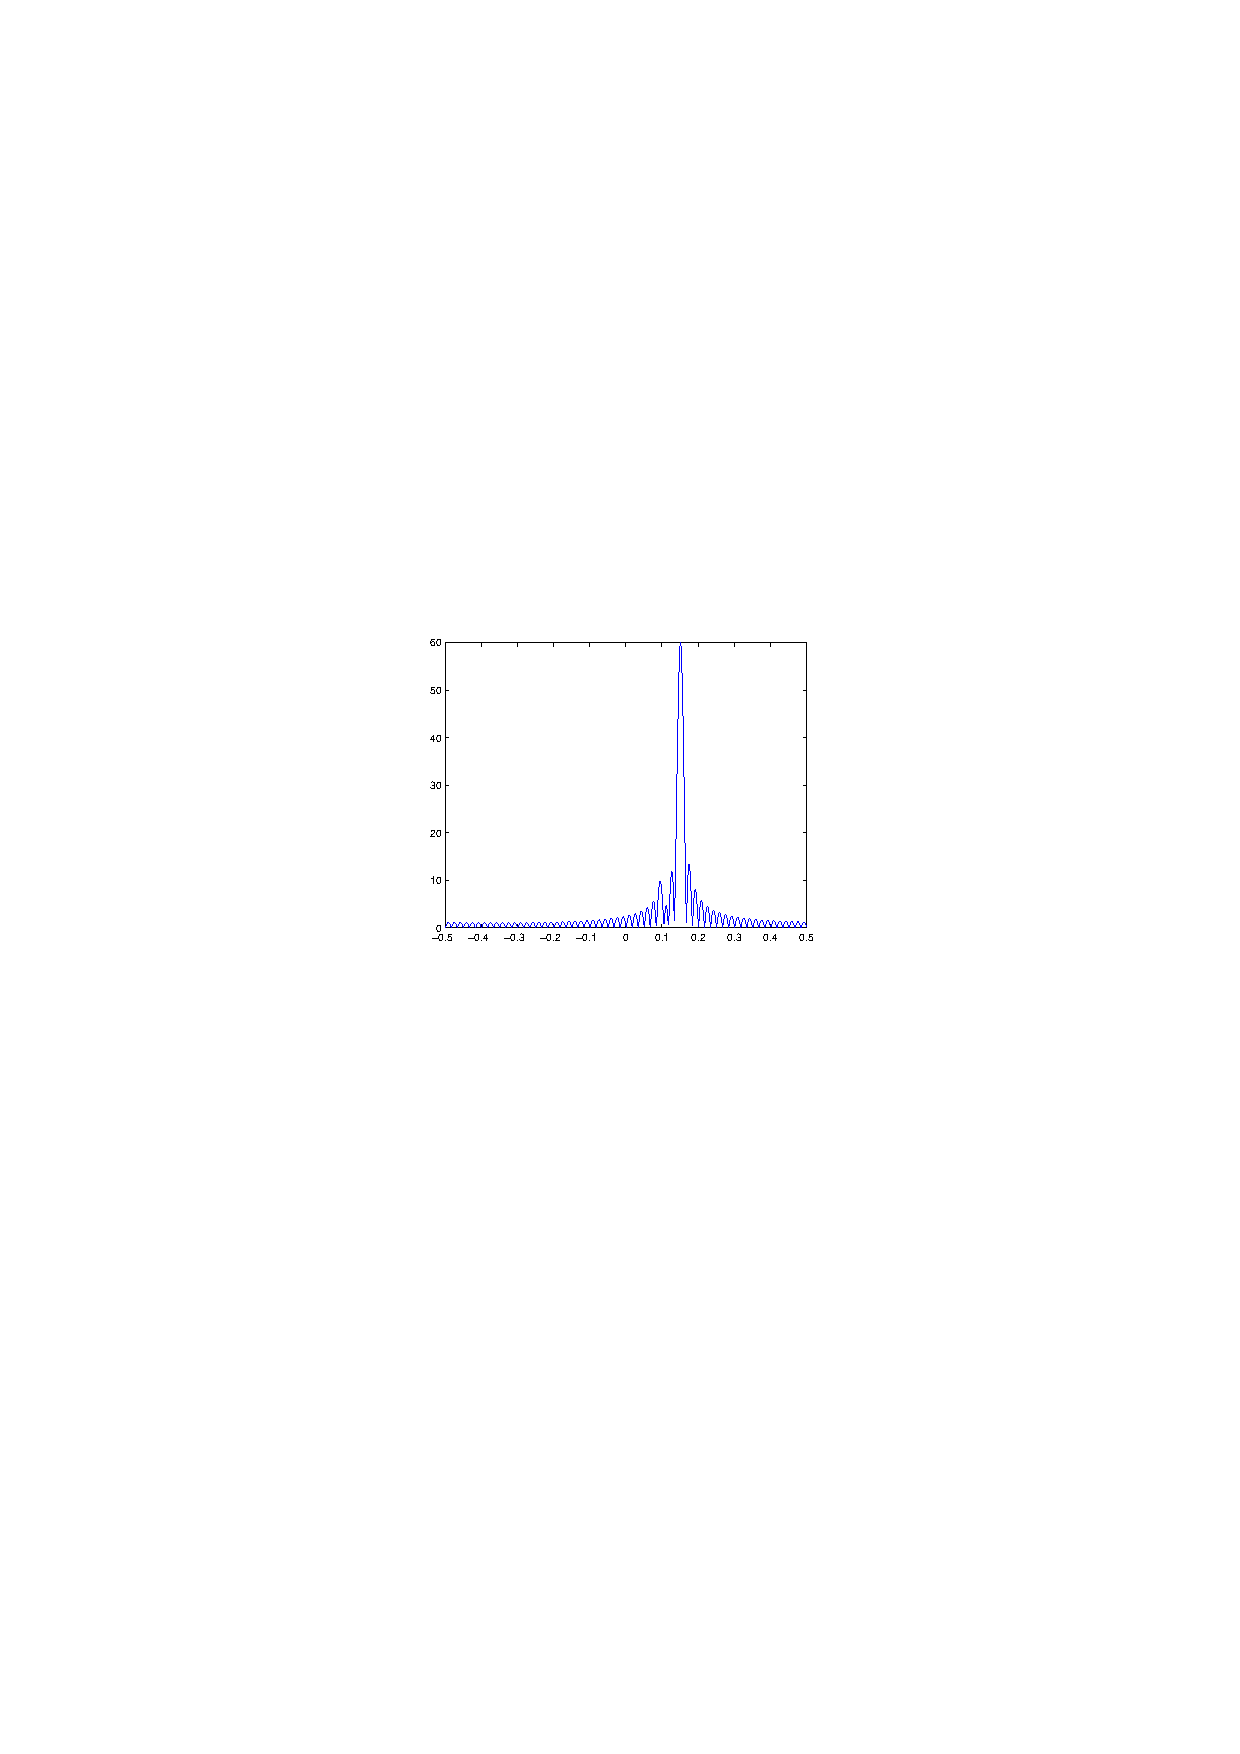
\includegraphics[width=0.6\textwidth]{Figures/Figure2-14}\\
  \caption{TFtD de la somme des deux ondes tronqu\'{e}es. Il est difficile de d\'{e}celer la pr\'{e}sence de l'harmonique complexe de faible amplitude.}\label{fig:figure2-14}
\end{figure}

On dit que $1/N$ est la r\'{e}solution fr\'{e}quentielle. Il faut augmenter $N$ pour pouvoir s\'{e}parer des fr\'{e}quences proches l'une de l'autre.


Les graphiques \Cref{fig:figure2-13} et \Cref{fig:figure2-13} montrent une situation o\`{u} $A_{1}$ est beaucoup plus grand que $A_{0}$. On constate que les lobes secondaires de la TFtD de l'harmonique complexe (tronqu\'{e}e) $\nu_{1}$ cachent jusqu'au lobe principal de l'harmonique complexe tronqu\'{e}e de fr\'{e}quence $\nu_{0}$. Cela est du au fait que la troncature choisie est trop brutale. Pour obtenir $u^{T}$ nous avons multipli\'{e} $u$ par une fen\^{e}tre rectangulaire que l'on va noter $c$:

$c_{n}=\left\{\begin{array}{l}
1\ \mathrm{s}\mathrm{i}\ 0\leq n<N\\
0\ \mathrm{s}\mathrm{i}\mathrm{n}\mathrm{o}\mathrm{n}
\end{array}\right.$
et on a fait $u^{T}=u.c$. Comme vu plus haut la TFtD de $u^{T}$ est la convolution de la
TFtD de $u$ avec celle de $c$.
\begin{figure}
  \centering
  % Requires \usepackage{graphicx}
  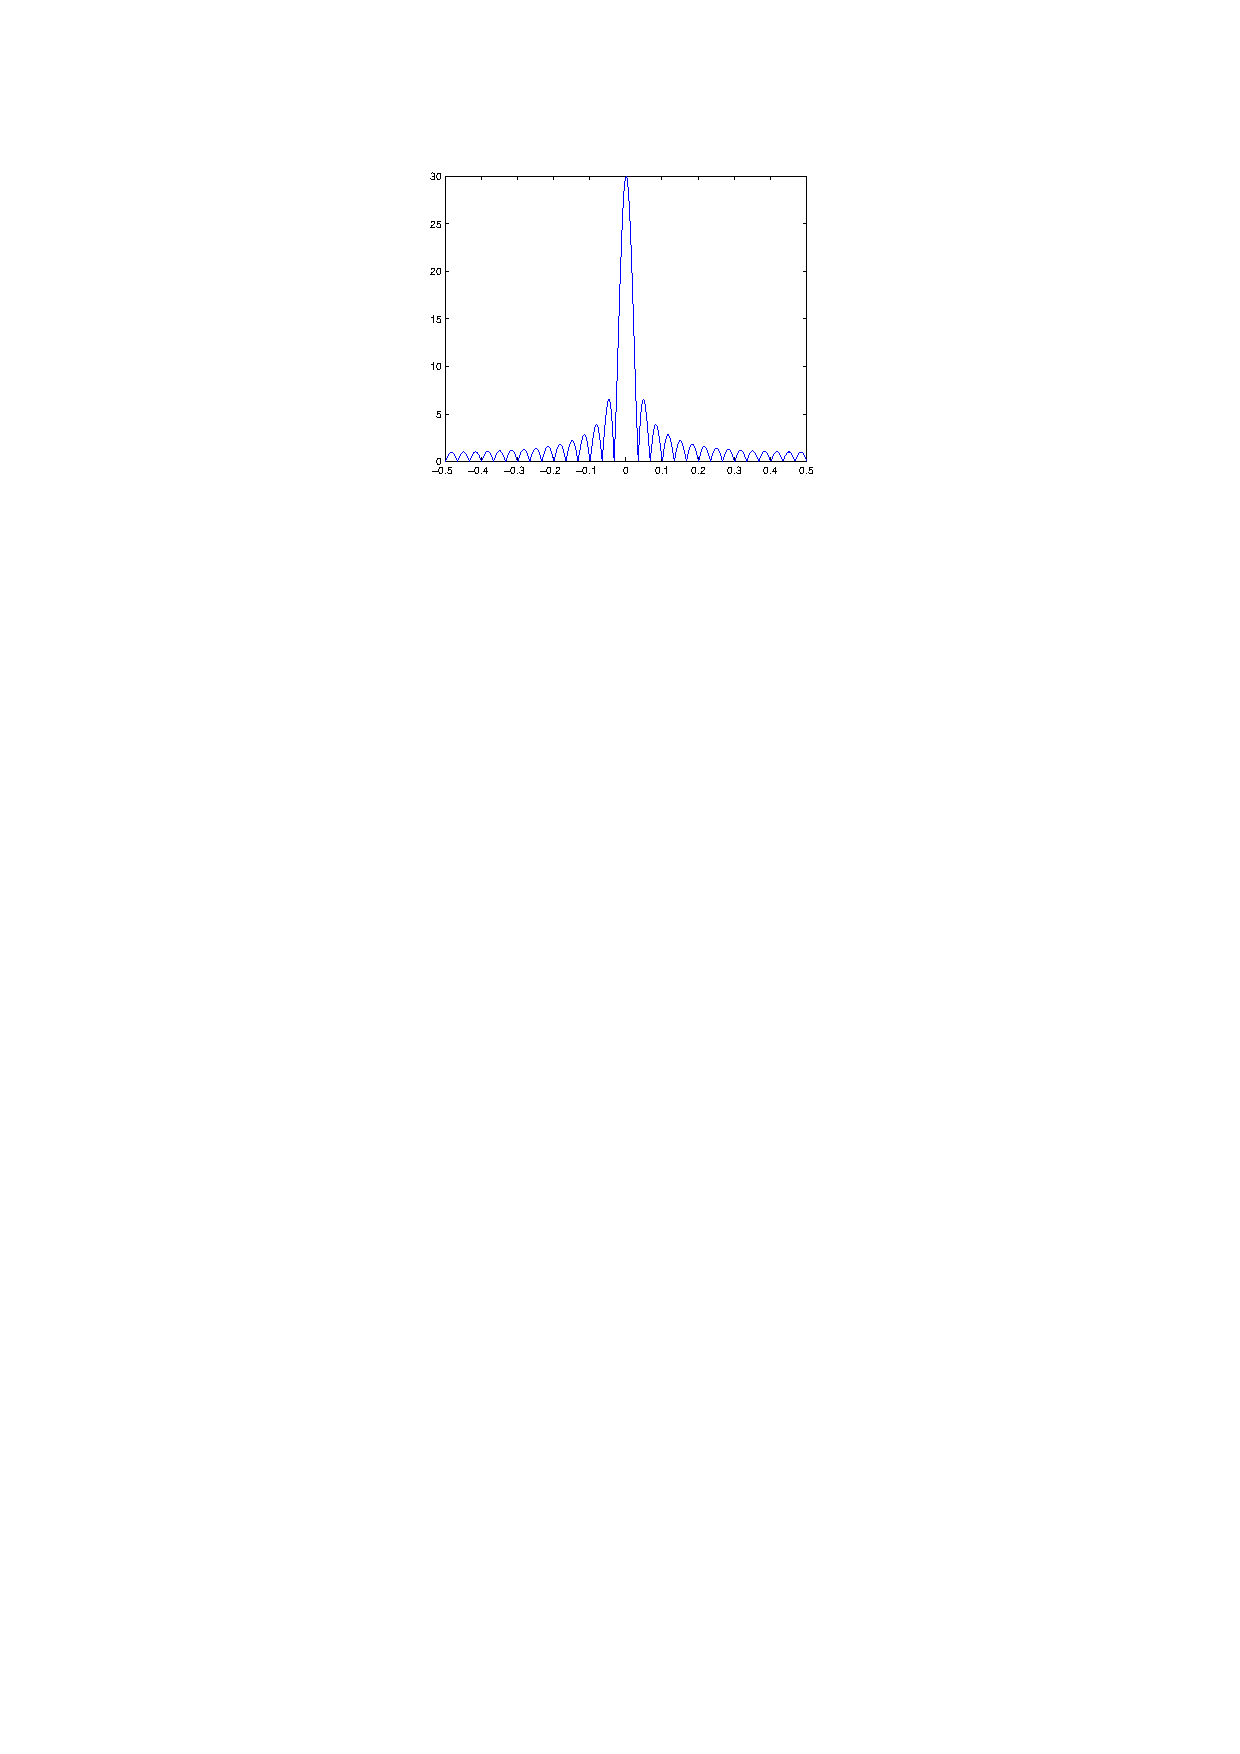
\includegraphics[width=0.6\textwidth]{Figures/Figure2-15}\\
  \caption{TFtD d'un cr\'{e}neau de taille 30.}\label{fig:figure2-15}
\end{figure}

\begin{figure}
  \centering
  % Requires \usepackage{graphicx}
  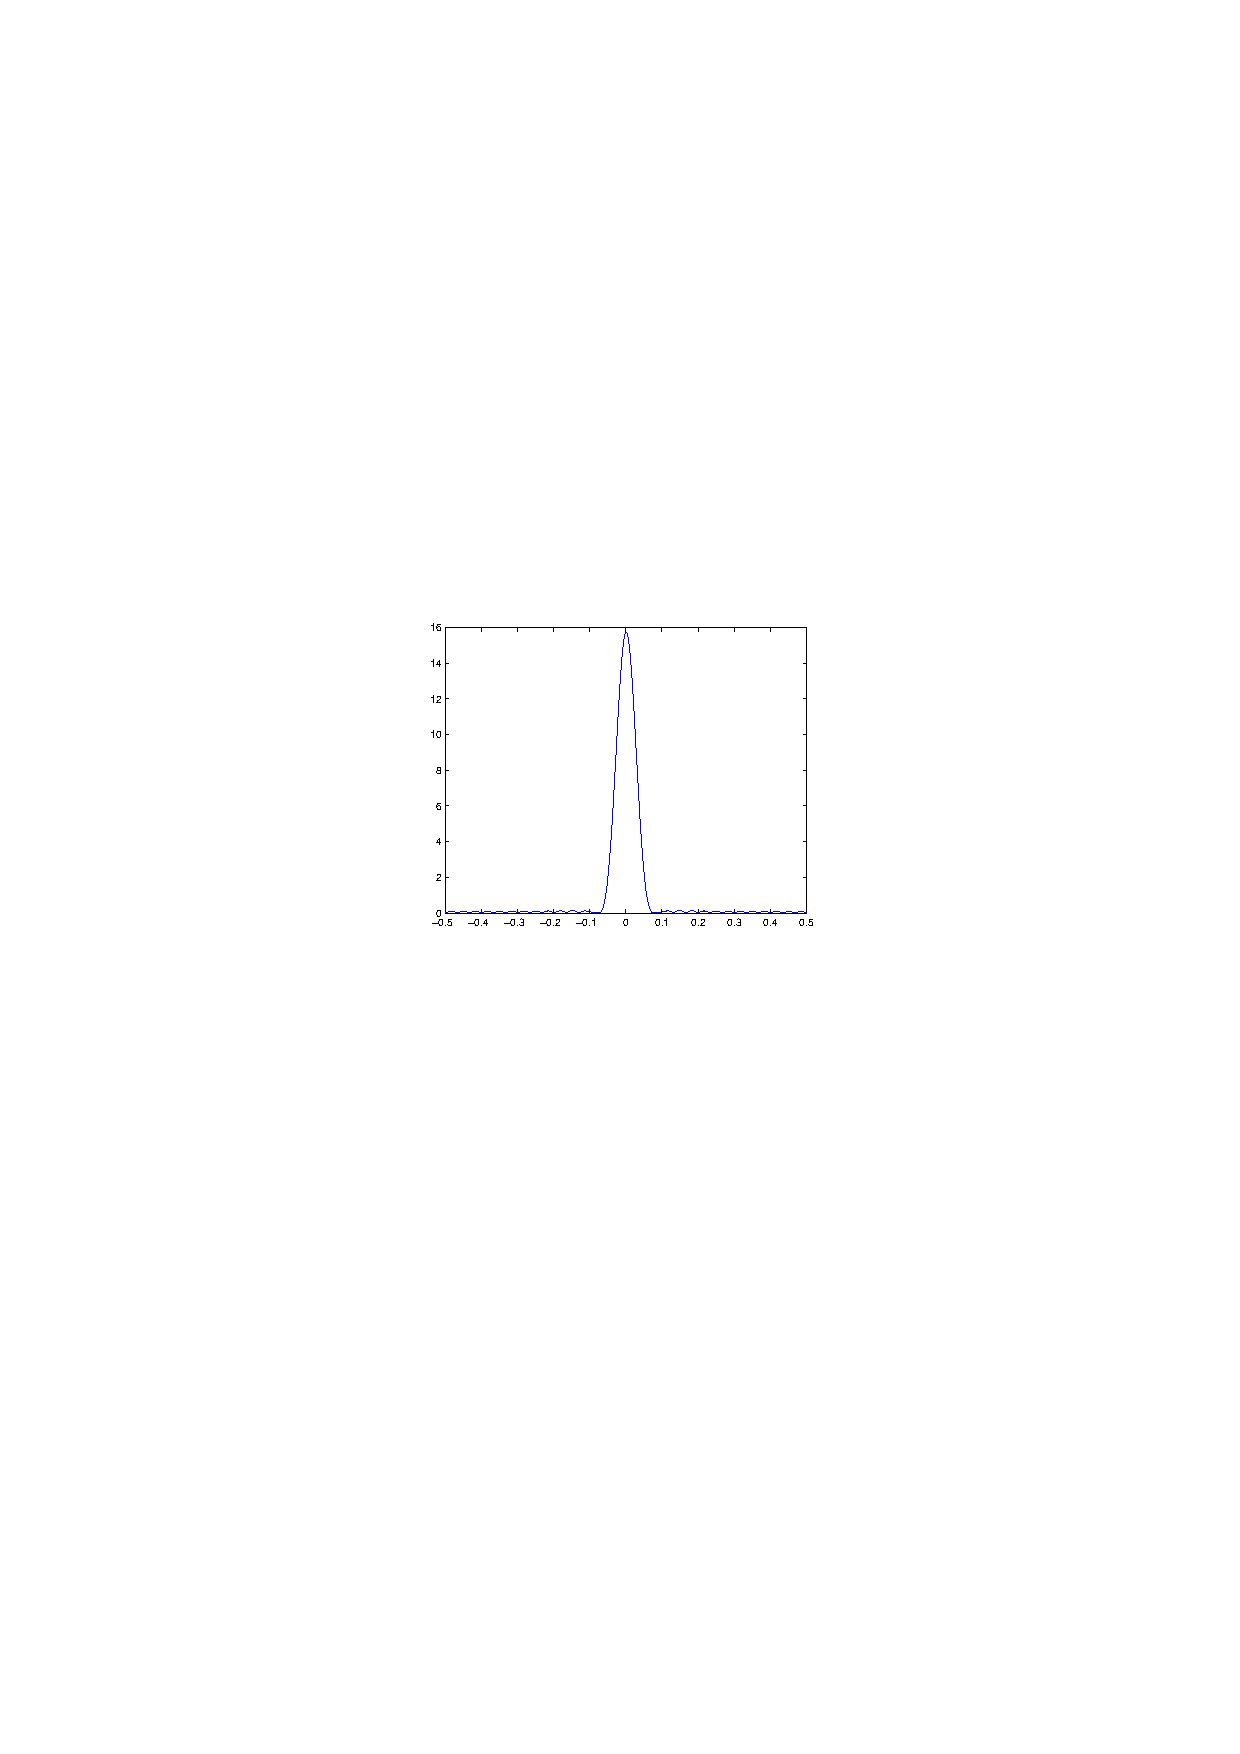
\includegraphics[width=0.6\textwidth]{Figures/Figure2-16}\\
  \caption{TFtD d'une fen\^{e}tre de Hamming de taille $N=30.$}\label{fig:figure2-16}
\end{figure}
\Cref{fig:figure2-15} montre le module de la TFtD de $c$. Si l'on trouve une fen\^{e}tre dont la TFtD pr\'{e}sente des lobes secondaires moins pro\'{e}minents on peut esp\'{e}rer r\'{e}soudre le probl\`{e}me que pose la s\'{e}paration des deux ondes de notre m\'{e}lange. Une fen\^{e}tre propos\'{e}e est la fen\^{e}tre de Hamming d\'{e}finit par

$h_{n}=\left\{\begin{array}{l}
0.\ 54-0.46cos(2\pi\frac{n}{N-1})\ \mathrm{s}\mathrm{i}\ 0\leq n<N\\
0\ \mathrm{s}\mathrm{i}\mathrm{n}\mathrm{o}\mathrm{n}
\end{array}\right.$

\Cref{fig:figure2-16} montre la TFtD de la fen\^{e}tre de Hamming.
Par rapport \`{a} celle de $c$ (cr\'{e}neau), on constate deux choses
\begin{enumerate}
\item Le lobe central est plus \'{e}tal\'{e} : ceci implique une perte de r\'{e}solution fr\'{e}quentielle. On passe d'une r\'{e}solution de l'ordre de $1/N$ \`{a} une r\'{e}solution de l'ordre de $2/N.$
\item Les lobes secondaires sont très atténués par rapport au  lobe central, ce qui permet de distinguer deux ondes dont les amplitudes diff\`{e}rent grandement.
\end{enumerate}
\Cref{fig:figure2-17}et \Cref{fig:figure2-18}  montrent comment la multiplication par une fen\^{e}tre de Hamming plut\^{o}t qu'une troncature brutale permet de distinguer une onde de faible amplitude.


\begin{figure}
  \centering
  % Requires \usepackage{graphicx}
  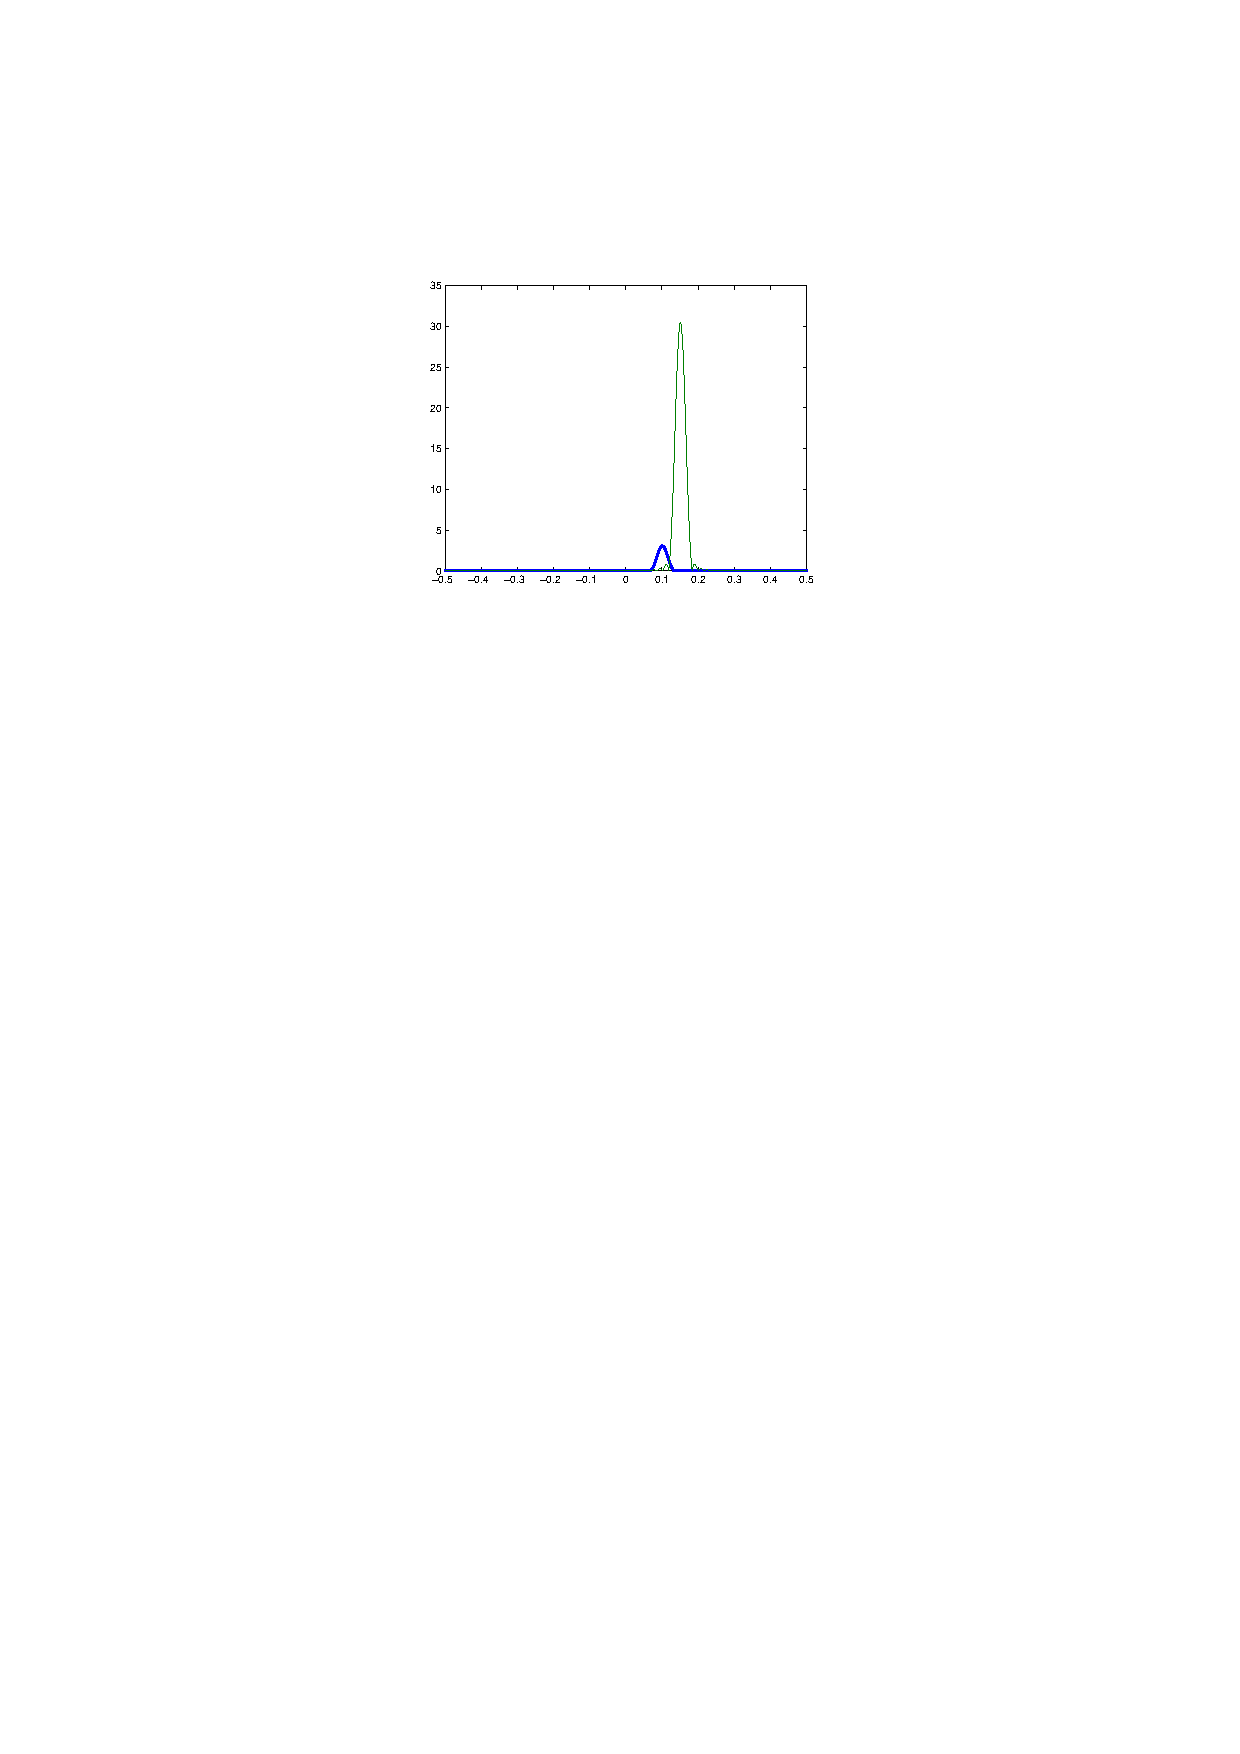
\includegraphics[width=0.6\textwidth]{Figures/Figure2-17}\\
  \caption{M\^{e}me figure que \Cref{fig:figure2-13} mais en ayant multipli\'{e} le signal par une fen\^{e}tre de Hamming. Cette fois l'harmonique complexe de faible amplitude est bien au dessus des lobes secondaires de l'harmonique complexe de forte amplitude.}\label{fig:figure2-17}
\end{figure}


\begin{figure}
  \centering
  % Requires \usepackage{graphicx}
  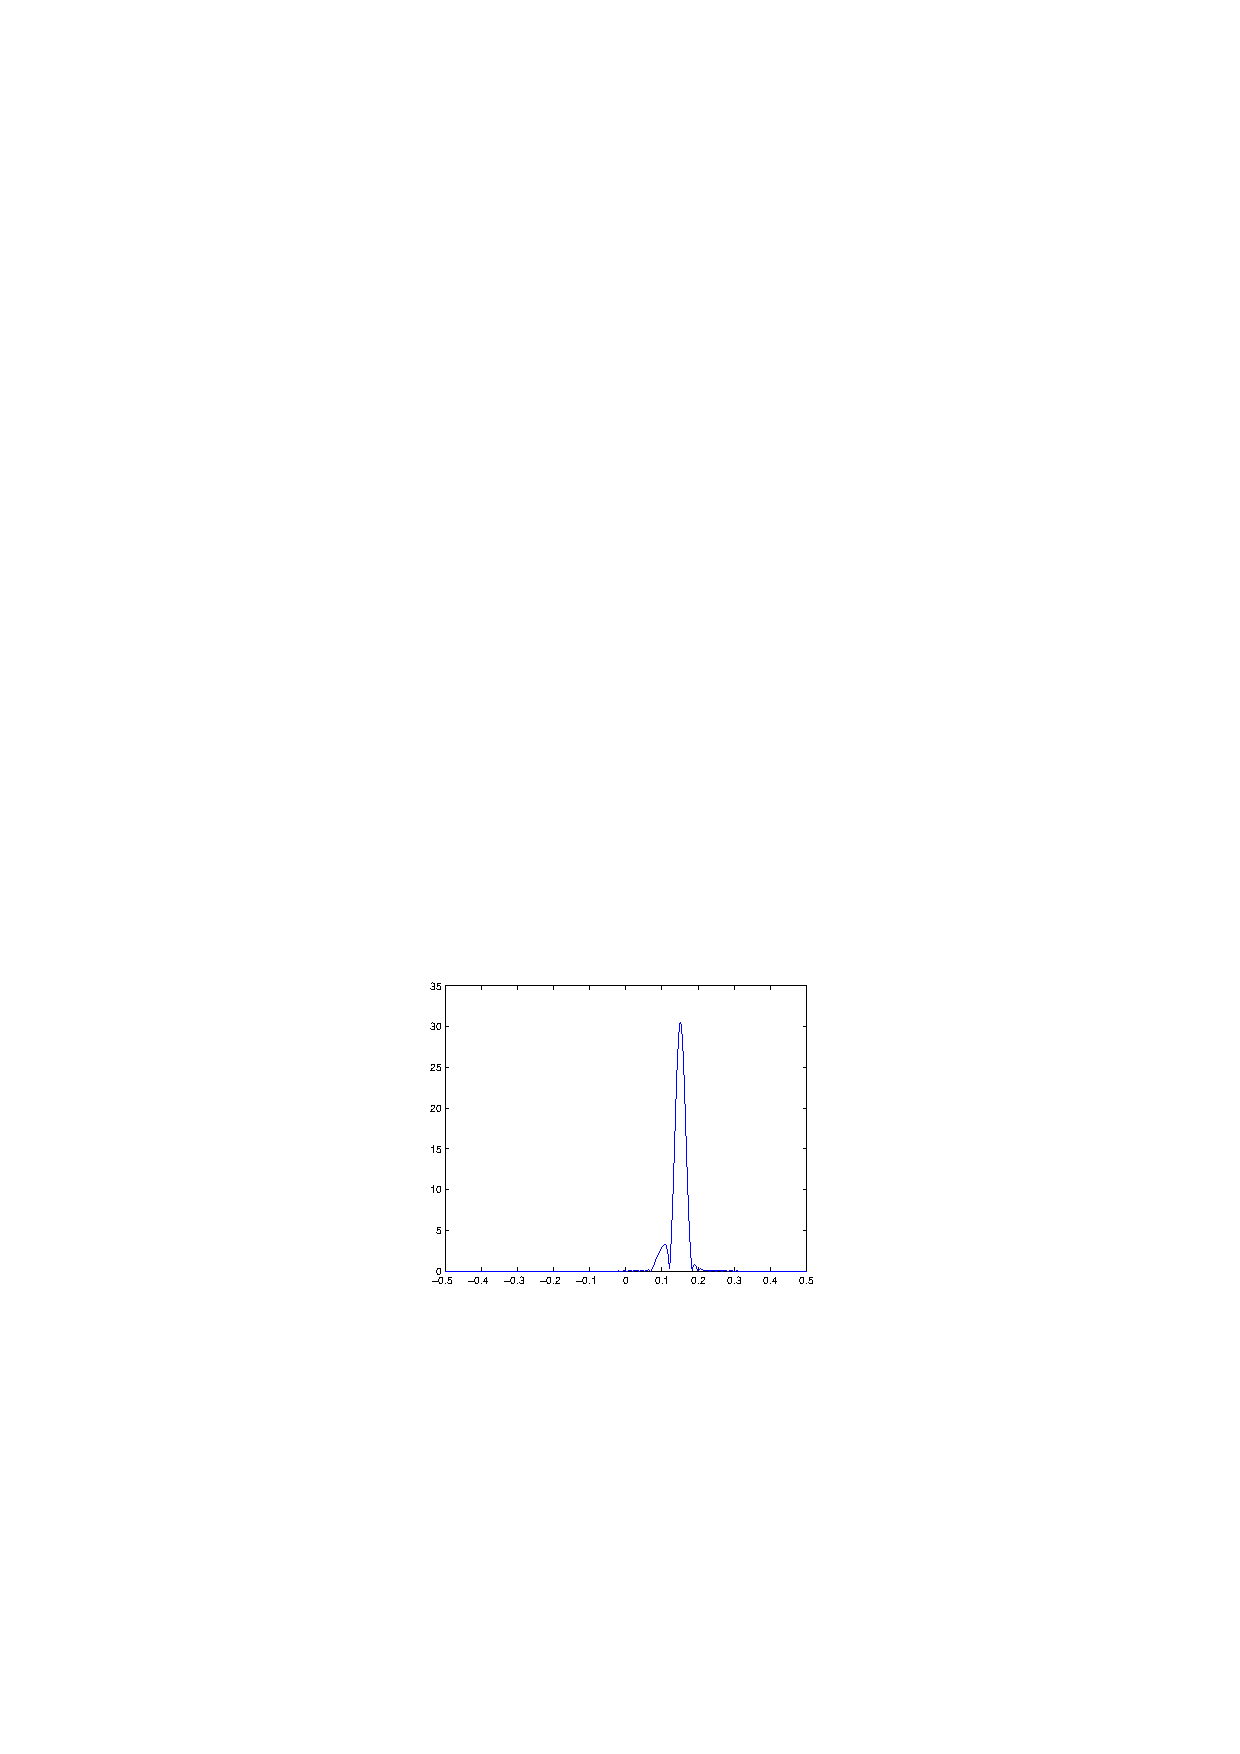
\includegraphics[width=0.6\textwidth]{Figures/Figure2-18}\\
  \caption{M\^{e}me figure que \Cref{fig:figure2-14} mais en ayant multipli\'{e} le signal contre une fen\^{e}tre de hamming plut\^{o}t que de la tronquer brutalement. Cette fois-ci on constate bien un deuxi\`{e}me lobe qui ne peut \^{e}tre confondu avec le lobe secondaire engendr\'{e} par l'harmonique complexe pr\'{e}dominante, car ces lobes secondaires sont bien plus faibles d'apr\`{e}s \Cref{fig:figure2-16}}\label{fig:figure2-18}
\end{figure}


\section{Transformée de Fourier à Court Terme (TFCT)}
La Transform\'{e}e de Fourier \`{a} Court Terme (TFCT) n'est pas \`{a} proprement parler une transformation de Fourier. Elle n'en a pas les propri\'{e}t\'{e}s alg\'{e}briques remarquables, c'est pourtant un outil essentiel en traitement du signal. Cet outil est bas\'{e} sur la constatation d\'{e}j\`{a} faite plus haut que le contenu fr\'{e}quentiel d'un signal peut \'{e}voluer au cours du temps. Elle se d\'{e}finit naivement comme une analyse locale des composantes fr\'{e}quentielles du si- gnal. Plus pr\'{e}cis\'{e}ment, pour chaque instant $n$, on extrait un certain nombre d'\'{e}chantillons du signal \'{e}tudi\'{e} autour du point $n$ que l'on \'{e}tudie par les moyens $\mathrm{v}\mathrm{u}\mathrm{s}$ ci-dessus (fen\^{e}trage et TFD d'ordres arbitraires).

Si $u$ est une suite d\'{e}finie sur $\zset$. On fixe une fen\^{e}tre $w_{0}, \ldots, w_{n}$ de taille
$N$ et on choisit un entier $M\geq N.$ La Transform\'{e}e de Fourier \`{a} Court Terme de $u$ de
fen\^{e}tre $w$ et de pr\'{e}cision $1/M$ est une fonction, que l'on note $U$ d\'{e}finie sur $\displaystyle \zset\times\frac{\{0,\ldots,M-1\}}{M}$par
$$
\forall(n,\ k)\in \zset\times\{0,\ \ldots,\ M-1\},\ U(n,\ \frac{k}{M})=\sum_{m\in \zset}u_{m}w_{n-m}\rme^{-2\rmi\pi \frac{k}{M}m}
$$
On peut aussi consid\'{e}rer $U$ comme une fonction d\'{e}finie sur $\displaystyle \zset \times \coint{-1/2,1/2}$ que l'on \'{e}chantillonnera aussi finement que l'on veut suivant la seconde variable en augmentant la valeur de $M$ (ordre de la $TFD$)
$$
\forall(n,\ \nu)\in \zset\times \coint{-1/2,1/2},\ U(n,\ \nu)=\sum_{m\in \zset}u_{m}w_{m-n}\rme^{-2\rmi\pi  1/m}
$$
On distingue cette notation de la notation $U$ pour la $TFD$ par le fait qu'elle dépend de deux variables.

\paragraph{Pour $n$ fix\'{e}}: On remarque que pour un entier $n$ fix\'{e}, la fonction $\nu\mapsto U(n,\ \nu)$ est la TFtD de la suite $l\mapsto u_{l}w_{l-n}$, c'est \`{a} dire la suite $u$ multipli\'{e}e par la $n$-translat\'{e}e de la fen\^{e}tre $w$. Il s'agit bien de ce que nous avions annonc\'{e}, autour de chaque instant $n$, on extrait une fenêtre de signal dont on calcule la TFtD (à l'aide d'une TFD dont le nombre de coefficients peut être choisi de façon arbitraire).

\paragraph{Pour $\nu$ fix\'{e}}: Pour une fr\'{e}quence $\nu$ fix\'{e}e avec $n$ variable, on a :
$$
U(n,\ \nu)=\sum_{m\in \zset}u_{m}w_{m-n}\rme^{-2\rmi\pi  1/m}=\rme^{-2\rmi\pi  1/n}\sum_{m}u_{m}\gamma_{n-m}
$$
o\`{u} $\gamma$ est la suite d\'{e}finie par
$$
\gamma_{l}=w_{-l} \rme^{2 \rmi\pi \nu l}
$$
Le module de $U$ est alors
$$
|U(n,\ \nu)|=|(u*\gamma)_{n}|
$$
Ainsi le module de $U$ est celui de la convolution de la sym\'{e}trique de $w$ multipli\'{e}e par une harmonique complexe  de fr\'{e}quence $\nu$. Cela signifie qu'\`{a} $\nu$ fix\'{e}, le module de $U$ refl\`{e}te \`{a} quel point la fr\'{e}quence $\nu$ est pr\'{e}sente dans le signal autour du point $n$. En effet, la TFtD de $\gamma$ est centr\'{e}e autour de la fr\'{e}quence $\nu$ (la fen\^{e}tre $w$, si c'est une fen\^{e}tre de Hamming par exemple, a son spectre centr\'{e} en z\'{e}ro).


Le spectrogramme est le module au carr\'{e} de la TFCT $((n,\ \nu)\mapsto|U(n,\ \nu)|^{2})$ . On le visualise comme une image, les deux axes sont ceux des variables $n$ et $\nu$, on repr\'{e}sente la valeur du spectrogramme soit en gris, suivant la valeur (sombre pour grand et clair pour faible).

\begin{figure}
  \centering
  % Requires \usepackage{graphicx}
  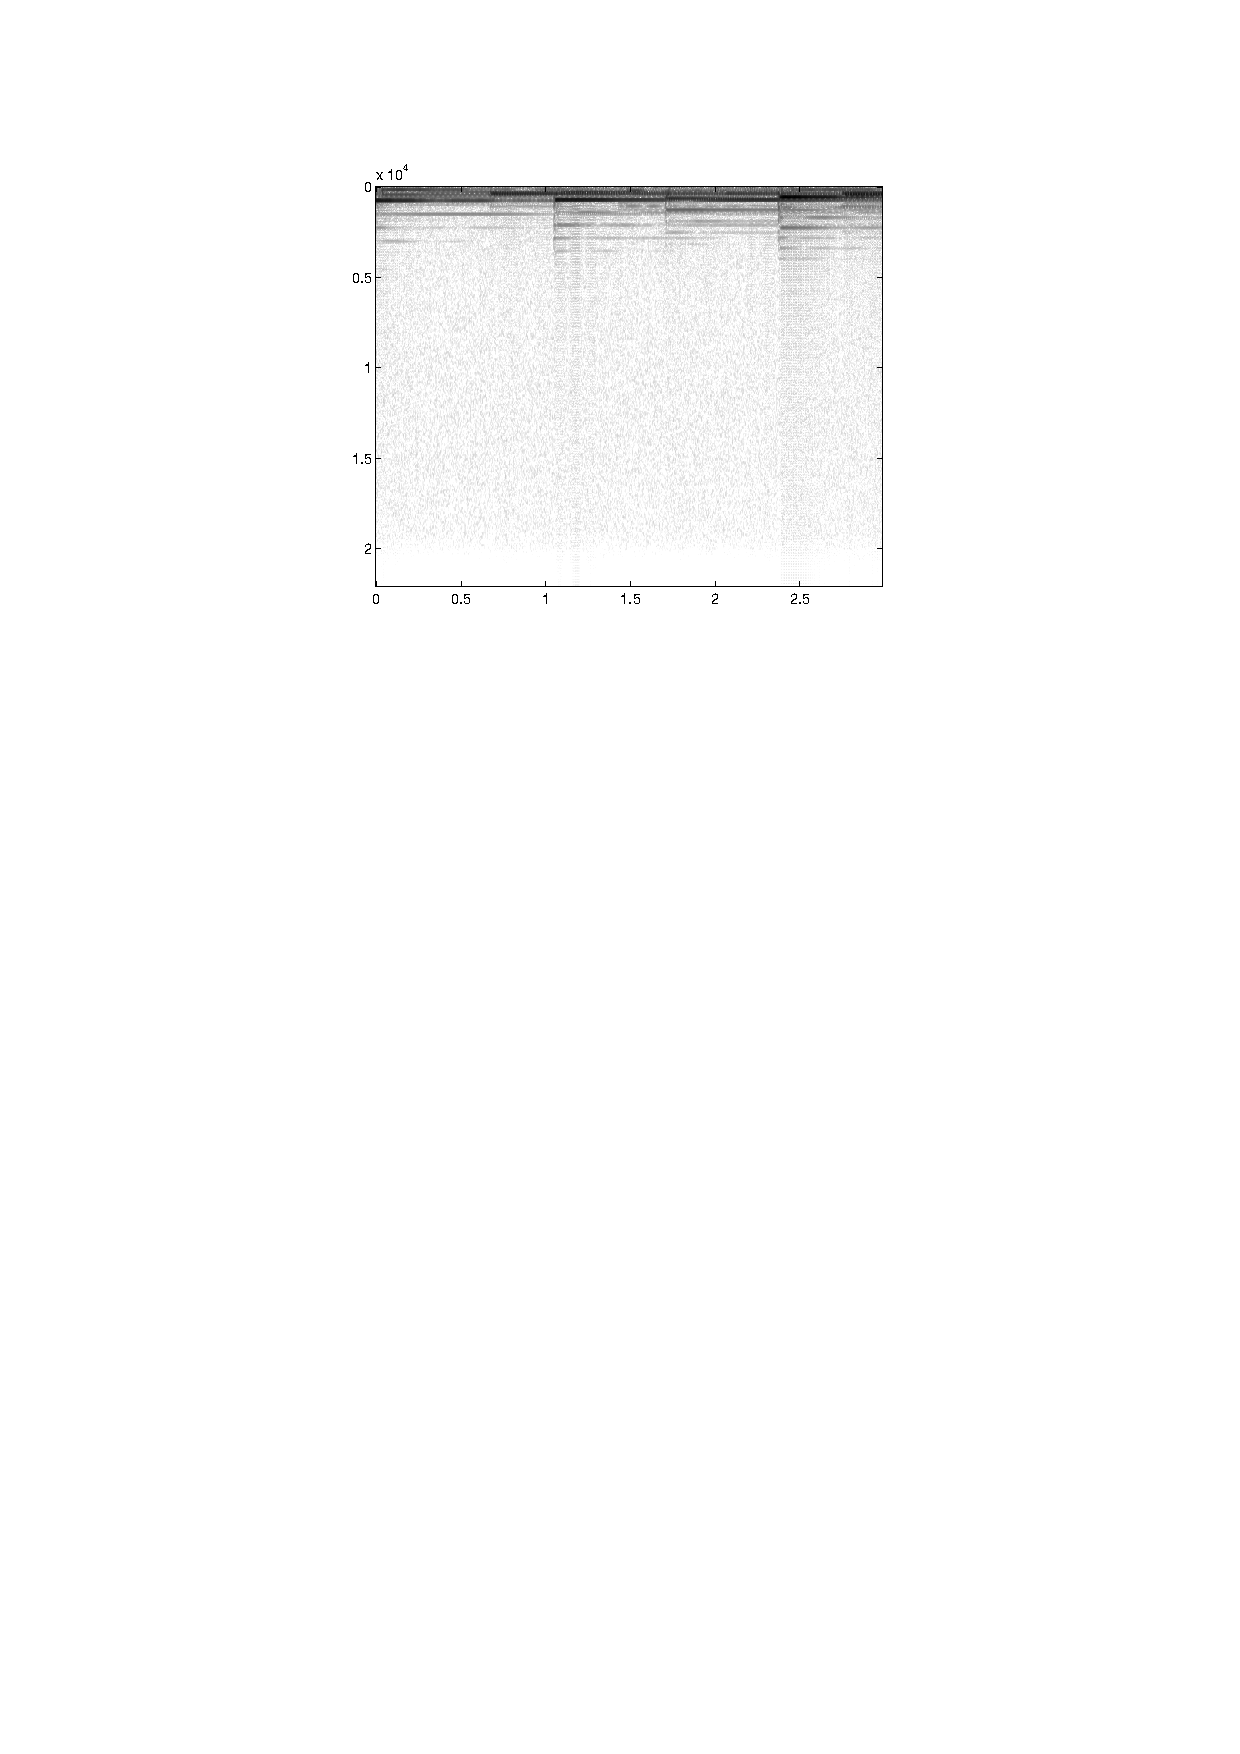
\includegraphics[width=0.6\textwidth]{Figures/Figure2-19}\\
  \caption{Spectrogramme d'un morceau de piano. On voit se succ\'{e}der les notes. Chaque note est caract\'{e}ris\'{e}e par l'apparition de raies qui s'affaiblissent \`{a} mesure que le son s'att\'{e}nue. (l'\'{e}chelle des fr\'{e}quences est du haut vers le bas et en $10000$ Hz d'unit\'{e})}\label{fig:figure2-19}
\end{figure}



\begin{figure}
  \centering
  % Requires \usepackage{graphicx}
  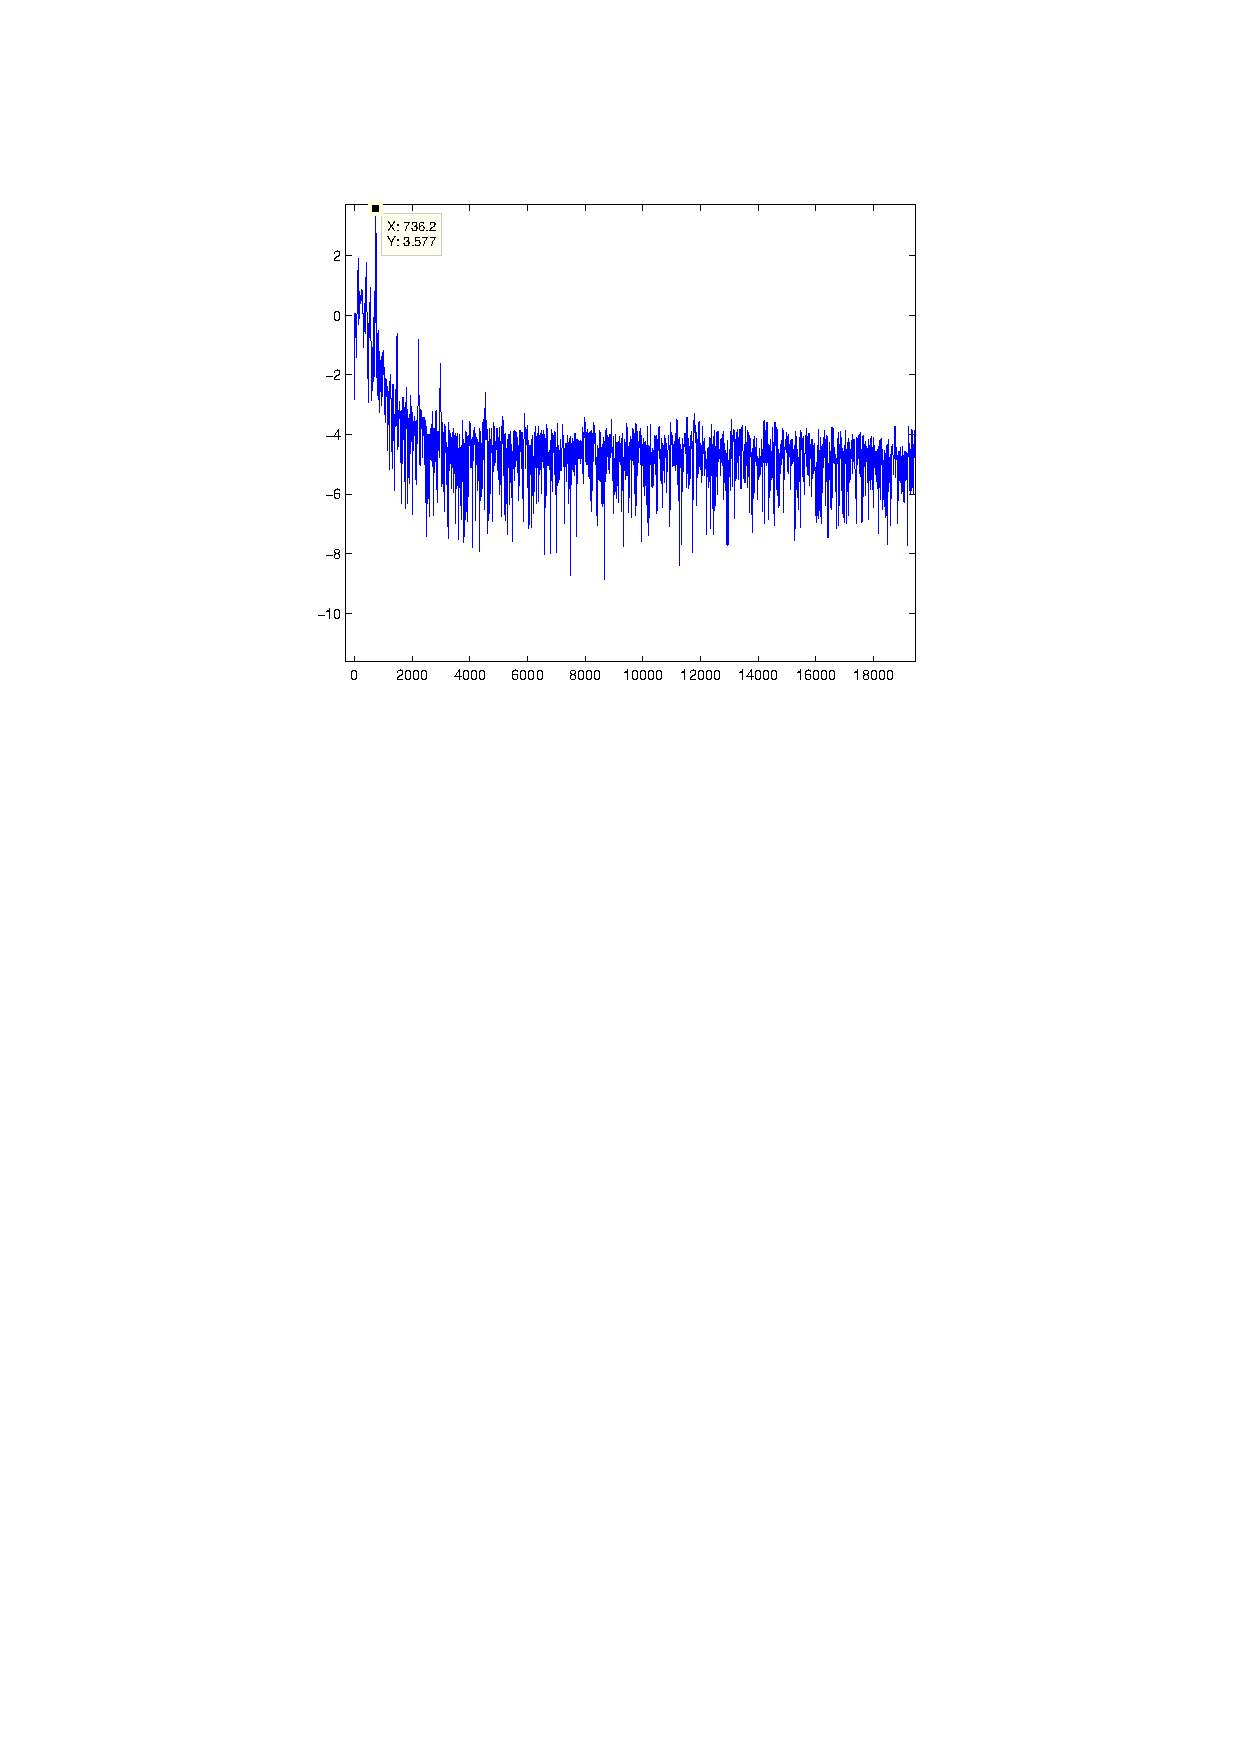
\includegraphics[width=0.6\textwidth]{Figures/Figure2-20}\\
  \caption{Une colonne du spectrogramme. C'est donc le contenu fr\'{e}quentiel local autour d'un certain instant. Le pic le plus pro\'{e}minent est pour la fr\'{e}quence $736$ Hz, qui correspond \`{a} peu pr\`{e}s \`{a} un Fa di\`{e}se.}\label{fig:figure2-20}
\end{figure}

i 
\chapter{Transformée en $z$ et filtrage}
\section{Transformée en $z$: définition}
\begin{definition}[Transformée en $z$]
\label{def:transformee}
La transform\'{e}e en $z$ d'une suite $\sequence{u}[n][\zset]$ est d\'{e}finie comme la s\'{e}rie $U(z)$ calcul\'{e}e comme suit:
\begin{equation}
\label{eq:definition-transformee}
U(z)=\sum_{n=-\infty}^{\infty} u_n z^{-n}
\end{equation}
o\`{u} $z$ est une variable complexe.
\end{definition}
On appelle encore \eqref{eq:definition-transformee} la transform\'{e}e directe, car c'est la relation qui permet d'obtenir $U(z)$ \`{a} partir de $\sequence{u}[n][\zset]$. Cette transfomée est bilatérale. L'op\'{e}ration inverse porte le nom de transformation inverse.

Comme cette transformation est une s\'{e}rie infinie, elle n'existe que pour les valeurs de $z$ pour lesquelles cette s\'{e}rie converge. La r\'{e}gion de convergence (RC) est l'ensemble des valeurs de $z$ pour lesquelles la s\'{e}rie prend une valeur finie. Dès lors, \emph{toute transform\'{e}e en $z$} doit \^{e}tre accompagnée de la région du plan complexe sur laquelle elle converge. Pour d\'{e}terminer la r\'{e}gion de convergence, on utilise le crit\`{e}re de Cauchy sur la convergence des s\'{e}ries entières. Rappelons que la s\'{e}rie à termes positifs
$ \sum_{n=0}^{\infty} v_n$ converge si
\begin{equation}
\label{eq:critere-cauchy}
\limsup_{n\rightarrow\infty} v_{n}^{1/n}<1 \eqsp.
\end{equation}
Pour appliquer le crit\`{e}re de Cauchy, on d\'{e}compose la s\'{e}rie en deux s\'{e}ries:
$$
U(z)\ =\ \sum_{n=-\infty}^{-1} u_n z^{-n}+\sum_{n=0}^{\infty} u_n z^{-n} = U_1(z) + U_2(z) \eqsp.
$$
L'application du crit\`{e}re de Cauchy \`{a} la s\'{e}rie $U_{2}(z)$ m\`{e}ne \`{a}
\begin{align*}
\limsup_{n\rightarrow\infty}| u_n z^{-n}|^{1/n}\ <\ 1  \quad \Rightarrow \quad
\limsup_{n\rightarrow\infty}| u_n |^{1/n}\ <\ |z|
\end{align*}
En appelant $R_{-}$ la limite
\begin{equation}
\label{eq:definition-R-}
R_{-}=\limsup_{n\rightarrow\infty}|u_n|^{1/n}
\end{equation}
la s\'{e}rie $U_{2}(z)$ converge sur la couronne $\ensemble{z \in \cset}{|z|>R_{-}}$.
Pour ce qui est de la s\'{e}rie $U_{1}(z)$ , apr\`{e}s un changement de variable, on a
$$
U_{1}(z)\ =\ \sum_{n=-\infty}^{-1} u_n z^{-n} =\ \sum_{n=1}^{\infty} u_{-n} z^{n}
$$
On a convergence si
\begin{align*}
\limsup_{n\rightarrow\infty}|u_{-n} z^{n}|^{1/n}\ <\ 1 \quad \Rightarrow \limsup_{n\rightarrow\infty}|u_{-n}|^{1/n}|z|\ <\ 1
\end{align*}
et donc la série $U_1(z)$ converge sur le disque
\begin{equation}
\label{eq:definition-R+}
|z|\ <\ \left\{ \lim_{n\rightarrow\infty}|u_{-n}|^{1/n} \right\}^{-1}=R+
\end{equation}
En toute g\'{e}n\'{e}ralit\'{e}, une s\'{e}rie converge donc  dans un anneau du plan complexe  donn\'{e} par
$$
R_{-}<|z|<R+
$$
Lorsque $R+\leq R_{-}$, le domaine de convergence est vide est la transformée en $z$ de la suite n'est alors pas défini.

La suite $U_{2}(z)$ repr\'{e}sente la transform\'{e}e en $z$ d'une \emph{suite causale}: les seules valeurs non-nulles de la suite
correspondent aux indices positifs. La transformée en $z$ d'une suite causale converge \`{a} l'ext\'{e}rieur d'un cercle de rayon $R_{-}$ donn\'{e} par \eqref{eq:definition-R-}.

La suite $U_{1}(z)$ repr\'{e}sente la transform\'{e}e en $z$ d'une suite anti-causale, c'est-\`{a}-dire ne comportant des \'{e}l\'{e}ments que pour les valeurs n\'{e}gatives de l'indice. En g\'{e}n\'{e}ral, une suite anti-causale converge \`{a} l'int\'{e}rieur d'un cercle de rayon $R_+$donn\'{e} par \eqref{eq:definition-R+}. Quand une suite est \`{a} dur\'{e}e limit\'{e}e, sa transform\'{e}e est donn\'{e}e par
\begin{equation}
\label{eq:z-duree-limitee}
U(z)=\sum_{n=n_{1}}^{n_{2}} u_n z^{-n}
\end{equation}
Pour autant que dans l'intervalle $[n_{1},\ n_{2}]$ le module de chaque \'{e}l\'{e}ment de la suite soit fini, la s\'{e}rie converge pour toutes les valeurs de $z$, sauf \'{e}ventuellement en $z=0$ ou $|z|\rightarrow\infty$. Les cas suivants peuvent \^{e}tre distingu\'{e}s:
\begin{enumerate}
\item si $n_{1}$ et $n_{2}$ sont positifs, on n'a pas convergence pour $z=0$ car les termes $z^{-n}$ divergent pour les $n$ positifs.
\item  si $n_{1}$ est n\'{e}gatif et $n_{2}$ est positif, on n'a pas convergence ni pour $z=0$ ni $|z|\rightarrow\infty$.
\item si $n_{1}$ et $n_{2}$ sont n\'{e}gatifs, on n'a pas convergence pour $|z|\rightarrow\infty$.
\end{enumerate}
Consid\'{e}rons les exemples suivants:
\begin{enumerate}
\item $u_n=\delta_n$ : la d\'{e}finition fournit directement $U(z)=1$. La transform\'{e}e existe partout.
\item $u_n=1$ si $n \geq 0$ et $u_n=0$ sinon :
$$
U(z)=\sum_{n=0}^{\infty}z^{-n}=\frac{1}{1-z^{-1}}
$$
pour $R_{-}=\displaystyle \lim_{n\rightarrow\infty}1^{1/n}=1^{1}$
\item $u_n=a^{n}$ pour $n \geq 0$, $u_n=0$ sinon
\begin{equation}
\label{eq:z-exponentiel}
\sum_{n=0}^{\infty}a^{n}z^{-n}=\sum_{n=0}^{\infty}(az^{-1})^{n}=\frac{1}{1-az^{-1}}
\end{equation}
avec un domaine de convergence $|z|>|a|$.
\item $u_n = \rme^{ 2 \rmi \pi \nu_0 n}$
$$
U(z)=\sum_{n=0}^{\infty}\rme^{2 \rmi \pi \nu_0 n}z^{-n}=\sum_{n=0}^{\infty}( \rme^{2 \rmi \pi \nu_0} z^{-1})^{n}=\frac{1}{1- \rme^{2 \rmi \pi \nu_0} z^{-1}}
$$
avec un domaine de convergence $|z|>1$.
\item La suite $u_n= a^n$ pour $n \in \zset$ n'a pas de transformée en $z$.
\end{enumerate}
\section{Transformée inverse}
Pour inverser une transform\'{e}e en $z$, on peut s'aider utilement du \emph{théorème de Cauchy} qui \'{e}tablit que
\begin{equation}
\label{eq:cauchy}
\frac{1}{2\pi \rmi}\oint_{\Gamma}z^{l-1}\rmd  z= \begin{cases} 1 & l= 0 \\ 0 & \text{sinon} \end{cases}
\end{equation}
o\`{u} $\Gamma$ est un contour qui entoure l'origine du plan et est parcouru dans le sens trigonométrique. En reprenant la d\'{e}finition de la transform\'{e}e en $z$ donn\'{e}e par \eqref{eq:definition-transformee}, en multipliant les deux membres par $z^{l-1}$ et en int\'{e}grant le long d'un contour entourant l'origine et appartenant au domaine de convergence, on trouve
\begin{align*}
\oint_{\Gamma}U(z)z^{l-1}\rmd z\ &=\ \oint_{\Gamma}\sum_{n=-\infty}^{\infty} u_n z^{-n+l-1}\rmd z \\
&=\ \sum_{n=-\infty}^{\infty} u_n \oint_{\Gamma}z^{-n+l-1}\rmd z
\end{align*}
o\`{u} l'interversion de l'int\'{e}grale et de la somme est licite compte tenu du fait que l'on op\`{e}re dans la zone de convergence de la transform\'{e}e. En utilisant le th\'{e}or\`{e}me de Cauchy \eqref{eq:cauchy}, on a finalement
\begin{equation}
\label{eq:inverse-z}
u_n=\frac{1}{2\pi \rmi}\oint_{\Gamma} U(z)z^{n-1}\rmd z
\end{equation}
avec les conditions d\'{e}j\`{a} \'{e}nonc\'{e}es \`{a} propos du contour d'int\'{e}gration.

L'\'{e}valuation de l'int\'{e}grale dans le plan complexe se fait \`{a} l'aide du th\'{e}or\`{e}me des r\'{e}sidus, qui \'{e}tablit que l'int\'{e}grale le long d'un contour est donn\'{e} par la somme des r\'{e}sidus de la fonction \`{a} int\'{e}grer, soit ici $U(z)z^{n-1}$, dans le contour $\Gamma$. Le r\'{e}sidu $r_{q}$ \`{a} un p\^{o}le d'ordre $q$ en $z=a$ est donn\'{e} par
\begin{equation}
\label{eq:residu-q}
r_{q}=\lim_{z\rightarrow a}\frac{1}{(q-1)!}\frac{\rmd ^{q-1}}{\rmd z^{q-1}}[U(z)z^{n-1}(z-a)^{q}]
\end{equation}
Pour un p\^{o}le simple $(q=1)$ en $z=a$, l'expression du r\'{e}sidu $r_{1}$ se r\'{e}duit \`{a}
\begin{equation}
\label{eq:residu-simple}
r_{1}=\lim_{z\rightarrow a}[U(z)z^{n-1}(z-a)]
\end{equation}
\begin{example}
Consid\'{e}rons la transform\'{e}e en $z$ donn\'{e}e par
$$
U(z)=\frac{1}{1-z^{-1}}
$$
et le domaine de convergence $|z|>1$. En utilisant la formule d'inversion, on a donc que
\begin{align*}
u_n\ =\ \frac{1}{2\pi \rmi}\oint_{\Gamma}\frac{z^{n-1}}{1-z^{-1}}\rmd z= \frac{1}{2\pi \rmi}\oint_{\Gamma}\frac{z^{n}}{z-1}\rmd z
\end{align*}
o\`{u} le contour $\Gamma$ peut \^{e}tre un cercle de rayon plus grand que l'unit\'{e}. Pour $n\geq 0$, on n'a qu'un p\^{o}le d'ordre 1 en $z=1$ qui est entour\'{e} par le contour. Le r\'{e}sidu en ce p\^{o}le est donn\'{e} par $r_{1}$ valant
$$
r_{1}=\lim_{z\rightarrow 1}[z^{n}]=1
$$
On a donc $u_n=1$ pour tout $n \geq 0$. En ce qui concerne $n<0$, on a cette fois un autre p\^{o}le d'ordre $(-n)$ en $z=0$.
L'application de la formule du r\'{e}sidu donne, pour $q=-n$,
$$
 r_{q}=\lim {z\rightarrow 0} \frac{1}{(q-1)!}\frac{\rmd ^{q-1}}{\rmd z^{q-1}}[\frac{1}{z-1}]=-1
$$
autre r\'{e}sidu vaut toujours 1 et la somme donne donc $0$.
Pour \'{e}vi- ter l'\'{e}valuation fastidieuse du r\'{e}sidu en un p\^{o}le d'ordre non \'{e}gal \`{a} un, on peut recourir \`{a} un changement de variable $w=1/z$. On \`{a} d\`{e}s lors que le domaine de convergence devient $|w|<1$, et l'int\'{e}grale \`{a} \'{e}valuer devient
\begin{align*}
u_n\ &=\ \frac{1}{2\pi j}\oint_{\Gamma}\frac{z^{n}}{z-1}\rmd  z \\
     &=\ \frac{1}{2\pi j}\oint_{\Gamma^{-}}\frac{w^{-n}}{w^{-1}-1}\frac{(-1)}{w^{2}}\rmd w\\
     &=\ \frac{1}{2\pi j}\oint_{\Gamma+}\frac{w^{-n-1}}{1-w}\rmd  w =\ 0
\end{align*}
o\`{u} le contour $\Gamma^{-}$ peut \^{e}tre un cercle de rayon inf\'{e}rieur \`{a} l'unit\'{e} et parcouru dans le sens anti-trogonométrique (à cause du changement de variable). Le contour $\Gamma^{+}$ est parcouru dans le sens trigonométrique et compense le signe -. Pour $n<0$, on n'a pas de p\^{o}le en $0$. Le seul p\^{o}le est en $w=1$ mais n'est pas entour\'{e} par le domaine d'int\'{e}gration qui doit appartenir au domaine de convergence, soit $|w|<1$. Aucun p\^{o}le n'est donc entour\'{e} et la somme des r\'{e}sidus est nulle.
\end{example}
\section{D\'{e}compositions en fractions simples}
En utilisant d'ores et d\'{e}j\`{a} la propri\'{e}t\'{e} de lin\'{e}arit\'{e} de la transform\'{e}e en $z$, qui sera vue plus loin, on peut d\'{e}composer une fonction de forme compliqu\'{e}e en une somme de fonctions simples, et prendre la transform\'{e}e inverse de chacun des \'{e}l\'{e}ments. Comme on le verra, de nombreux syst\`{e}mes requi\`{e}rent l'\'{e}tude de transform\'{e}es du type
\begin{equation}
\label{eq:definition-U}
U(z)=P(z)/Q(z)
\end{equation}
o\`{u} $P$ et $Q$ sont des polyn\^{o}mes en $z$ ou $z^{-1}$. On peut alors d\'{e}composer $U(z)$ en fractions simples et obtenir la transform\'{e}e inverse par la somme des transform\'{e}es inverses. La transform\'{e}e peut se mettre sous la forme
$$
U(z)=S(z)+P_{0}(z)/Q(z)
$$
o\`{u} le degr\'{e} de $P_{0}(z)$ est inf\'{e}rieur \`{a} celui de $Q(z)$ . En fait, $S(z)$ et $P_{0}(z)$ sont respectivement le quotient et le reste de la division de $P$ par $Q$. Si le degr\'{e} de $P$ est inf\'{e}rieur \`{a} celui de $Q$, le quotient $S$ est nul.

Lorsque les racines $p_{i}$ de $Q(z)$ , appel\'{e}es p\^{o}les sont simples, on peut mettre le quotient sous la forme
\begin{equation}
\label{eq:decomposition-pole-simple}
P_{0}(z)/Q(z)=\sum_{i=1}^{N}\frac{\alpha_{i}}{z-p_{i}}
\end{equation}
Pour obtenir les poids $\alpha_{i}$, il suffit d'effectuer le calcul suivant:
$$
\alpha_{i}=[(z-p_{i})P_{0}(z)/Q(z)]_{z=p_{i}} \eqsp.
$$
Si un p\^{o}le $p_{n}$ est d'ordre $q>1$, la d\'{e}composition prend la forme
$$
P_{0}(z)/Q(z)=\sum_{i=1,\neq n}^{N}\frac{\alpha_{i}}{z-p_{i}}+\sum_{j=1}^{q}\frac{\beta_{j}}{(z-p_{n})^{j}}
$$
avec
$$
\beta_{j}=\frac{1}{(q-j)!}\frac{\mathrm{d}^{q-j}}{\mathrm{d}z^{q-j}}[(z-p_{n})^{j}P_{0}(z)/Q(z)]_{z=p_{n}}\text{   }(2.40)
$$
En r\'{e}alit\'{e}, il est plus int\'{e}ressant d'obtenir des fractions o\`{u} $z^{-1}$ apparaît au
d\'{e}nominateur, car les fractions dans ce cas correspondent directement \`{a} des
transform\'{e}es connues. D\`{e}s lors, tout ce qui vient d'\^{e}tre dit est appliqu\'{e} pour
des polyn\^{o}mes en $z^{-1}$ et non pas en $z$.

\begin{example}
Consid\'{e}rons la transform\'{e}e donn\'{e}e par
$$
U(z)=\frac{1}{1-3z^{-1}+2z^{-2}}
$$
pour $|z|>2$. Comme nous consid\'{e}rons que la variable est $z^{-1}$, le degr\'{e} du num\'{e}rateur est bien inf\'{e}rieur \`{a} celui du d\'{e}nominateur.
Les p\^{o}les sont donn\'{e}s par $z^{-1}=1$ et $z^{-1}=0.5$. On recherche donc une d\'{e}composition en fractions simples du type
\begin{align*}
U(z)\ &= \frac{0.5}{(z^{-1}-1)(z^{-1}-0.5)} \\
      &=\ \frac{\alpha_{1}}{z^{-1}-1}+\frac{\alpha_{2}}{z^{-1}-0.5}
\end{align*}
On trouve en utilisant ce qui a \'{e}t\'{e} vu pr\'{e}c\'{e}demment,
$$
U(z)=\frac{1}{z^{-1}-1}+\frac{-1}{z^{-1}-0.5}
$$
D\`{e}s lors,
$$
U(z)=\frac{2}{1-2z^{-1}}-\frac{1}{1-z^{-1}}
$$
et il est possible d'identifier ces fractions au r\'{e}sultat obtenu en \eqref{eq:z-exponentiel}. On trouve de ce fait
$$
u_n=2\times 2^{n} \1_{\nset}(n) - \1_{\nset}(n)=(2^{n+1}-1) \1_{\nset}(n) .
$$
Si on avait consid\'{e}r\'{e} les polyn\^{o}mes comme des fonctions de $z$, on aurait eu
\begin{align*}
U(z) &=\ \frac{1}{1-3z^{-1}+2z^{-2}} \\
     &=\ \frac{z^{2}}{z^{2}-3z+2}\\
     &=\ 1+\frac{3z-2}{z^{2}-3z+2}\\
     &=\ 1+\frac{3z-2}{(z-2)(z-1)}\\
     &=\ 1+\frac{4}{(z-2)}+\frac{-1}{(z-1)}\\
     &=\ 1+\frac{4z^{-1}}{(1-2z^{-1})}-\frac{1}{(1-z^{-1})}
\end{align*}
En s'aidant de la propri\'{e}t\'{e} de d\'{e}calage qui sera vue plus loin, on a que
$$
u_n=\delta_n +4\times 2^{n-1} \1_{\nset}(n-1)-\1_{\nset}(n-1) \eqsp.
$$
Cette forme est moins concise que la pr\'{e}c\'{e}dente.
\end{example}
\section{Propri\'{e}t\'{e}s de la transform\'{e}e en $z$}
\subsection{Lin\'{e}arit\'{e}}
La lin\'{e}arit\'{e} de la transformation signifie que la transform\'{e}e d'une suite obtenue par combinaison lin\'{e}aire d'autres suites n'est rien d'autre que la combinaison lin\'{e}aire des transform\'{e}es correspondantes. Sidonc
$$
u_n=a x_n +b y_n
$$
alors
\begin{align*}
U(z)\ &=\ \sum_{n=-\infty}^{\infty} u_n z^{-n} =\ a\ \sum_{n=-\infty}^{\infty}x_{n} z^{-n}+b\sum_{n=-\infty}^{\infty} y_n z^{-n} \\
&=\ a\ X(z)+bY(z)
\end{align*}
La r\'{e}gion de convergence est au moins l'intersection des r\'{e}gions associ\'{e}es \`{a} $X(z)$ et $Y(z)$ car la combinaison lin\'{e}aire peut introduire des z\'{e}ros qui compensent certains p\^{o}les.

\subsubsection{D\'{e}calage et transform\'{e}e bilat\'{e}rale}
Soit
$$
v_n =u_{n-n_{0}}
$$
La transform\'{e}e en $z$ de $\sequence{v}[n][\zset]$ est donn\'{e}e par
\begin{align*}
V(z) &=\ \sum_{n=-\infty}^{\infty} v_n z^{-n} \\
     &=\ \sum_{n=-\infty}^{\infty}u_{n-n_0}z^{-n} \\
     &=\ \sum_{m=-\infty}^{\infty}u_n z^{-(m+n_{0})} \\
     &=\ z^{-n_{0}} U(z)
\end{align*}
Le domaine de convergence est le m\^{e}me celuide $U(z)$ sauf que si $n_{0}$ est positif (resp. n\'{e}gatif), on a un p\^{o}le en $0$ (resp. $ z\rightarrow\infty$). Il peut y avoir des compensations de z\'{e}ros ou p\^{o}les.

Multiplier une transform\'{e}e en $z$ par $z^{-1}$ revient donc \`{a} retarder la suite d'une unit\'{e} (p\'{e}riode d'\'{e}chantillonnage). On se r\'{e}f\`{e}re souvent \`{a} $z^{-1}$ comme op\'{e}rateur de retard unit\'{e}.

La propri\'{e}t\'{e} de d\'{e}calage permet de traiter les \'{e}quations aux diff\'{e}rences vues pr\'{e}c\'{e}demment. A partir de
$$
v_n = u_n - \sum_{k=1}^p b_k u_{n-k}
$$
on trouve par transformation en $z$,
\begin{align*}
V(z) &=\ U(z)- \sum_{k=1}^p b_{k}z^{-k}V(z)
\end{align*}
ce qui implique que
\[
V(z) =\frac{U(z)}{1+ \sum_{k=1}^p b_{k}z^{-k}}
\]
Il faut faire attention toutefois avec ce calcul "formel" que les régions de convergence de $U(z)$ et de $1/ (1 + \sum_{k=1}^p b_k z^{-k})$ soient compatibles. Nous reviendrons sur cet aspect plus loin dans l'exposé.
\subsubsection{D\'{e}calage et transform\'{e}e unilat\'{e}rale}
Dans le cas unilat\'{e}ral, il faut \^{e}tre plus prudent dans ce que l'on \'{e}crit. La transformée unilatérale de la suite $\sequence{u}[n][\zset]$ est donnée par
\begin{equation}
\label{eq:transformee-unilaterale}
\tilde{U}(z)= \sum_{k=0}^\infty u_k z^{-k}\eqsp.
\end{equation}
Notons que nous ne calculons la somme que pour les indices positifs ! Le rayon de convergence de la transfomrmée monolatérale est une couronne
donnée ${z \in \cset}{|z| \geq \limsup_{n \to \infty} |u_n|^{1/n}}$.
Si on pose $v_n=u_{n-1}$ , la transform\'{e}e bilat\'{e}rale est calcul\'{e}e par
\begin{align}
\nonumber
\tilde{V}(z)\ &=\ \sum_{n=0}^{\infty}v_nz^{-n} \\
\nonumber
&=\ \sum_{n=0}^{\infty}u_{n-1}z^{-n} \\
\nonumber
&=\ z^{-1}\sum_{m=-1}^{\infty} u_m z^{-m} \\
\nonumber
&=\ z^{-1}[u_{-1} z+\tilde{U}(z)] \\
&=\ u_{-1}+z^{-1}\tilde{U}(z)
\label{eq:decalage-unilateral}
\end{align}
On voit donc qu'un d\'{e}calage vers la droite permet de faire appara\^{i}tre des \'{e}l\'{e}ments qui ne sont pas pris en consid\'{e}ration par la transformation unilatérale de d\'{e}part. Cette propri\'{e}t\'{e} permet de prendre en compte les conditions initiales non nulles.
Soit
\[
v_n=u_n+av_{n-1}\
\]
avec $v_{-1}=K$ et une excitation $u_n=\rme^{2 \rmi \pi \nu_0 n} \1_{\nset}(n)$ . En vertu de \eqref{eq:decalage-unilateral}
la transform\'{e}e en $z$ donne
\begin{align*}
\tilde{V}(z)\ &=\ \tilde{U}(z)+av_{-1}+az^{-1}\tilde{U}(z) \\
&=\ \frac{\tilde{U}(z)+av_{-1}}{1-az^{-1}} \\
&=\ \frac{aK}{1-az^{-1}}+\frac{1}{(1-az^{-1})(1- \rme^{2 rmi \pi \nu_{0}}z^{-1})} \\
& =\ \frac{aK}{1-az^{-1}}+\frac{1}{(1-\rme^{2 \rmi \pi nu_{0}}/a)(1-az^{-1})}
+ \frac{1}{(1-a/\rme^{2 \rmi \pi \nu_{0}})(1-\rme^{2 rmi \pi \nu_{0}}z^{-1})} \\
&=\ \frac{aK}{1-az^{-1}}+\frac{a}{(a-\rme^{2 \rmi \pi \nu_{0}})(1-az^{-1})}
+\ \frac{\rme^{2 \rmi \pi \nu_{0}}}{(\rme^{2 \rmi \pi \nu_{0}}-a)(1-\rme^{2 \rmi \pi\nu_{0}}z^{-1})}
\end{align*}
De ce fait, en utilisant les transform\'{e}es inverses d\'{e}j\`{a} \'{e}tablies, on
trouve
\[
v_n=\1_\nset(n)[a^{n+1}K+\frac{a^{n+1}}{a-\rme^{2 \rmi \pi \nu_{0}}}-\frac{\rme^{2 \rmi \pi \nu_{0}(n+1)}}{a-\rme^{2 \rmi \pi \nu_{0}}}]\
\]
La premi\`{e}re partie de la r\'{e}ponse correspond \`{a} la r\'{e}ponse libre, c'est-
\`{a}-dire l'\'{e}volution du syst\`{e}me sous l'effet des conditions initiales.
La seconde partie correspond \`{a} la partie transitoire de la r\'{e}ponse
forc\'{e}e. La troisi\`{e}me partie correspond \`{a} la r\'{e}ponse de r\'{e}gime de la
r\'{e}ponse forc\'{e}e.

On peut bien \'{e}videmment g\'{e}n\'{e}raliser ce qui pr\'{e}c\`{e}de au cas de plusieurs conditions initiales.

%Changement d'\'{e}chelle
%
%Si on effectue un changement de variable complexe $w=az$ o\`{u} $a$ peut \^{e}tre complexe, le domaine de convergence est modffi\'{e} comme suit
%$$
%R_{-}\ <\ |z|<R+
%$$
%$$
%R_{-}\ <\ |w/a|<R+
%$$
%$$
%|a|R_{-}\ <\ |w|<|a|R+\text{   }(2.58)
%$$
%De plus, si la transform\'{e}e en $z$ poss\`{e}de un p\^{o}le en $z=p$, la transform\'{e}e ex- prim\'{e}e \`{a} l'aide de $w$ poss\`{e}de un p\^{o}le en $w=az=ap$. On voit donc qu'un tel changement de variable permet de modffier la position des p\^{o}les, tant en amplitude qu'en phase puisque la multiplication se fait par un complexe.
%
%26
%
%{\it CHAPITRE 2. LA TRANSFORM\'{E}E EN} $Z$
%
%1. si $a$ est r\'{e}el et positif, on rapproche le p\^{o}le de l'origine si $a<1$ et on l'\'{e}loigne si $a>1$.
%
%2. si $a$ est complexe du type $e^{j\theta}$, le p\^{o}le subit une rotation de $\theta$ radians au- tour de l'origine.
%
%On peut se demander quelle est la suite qui correspond \`{a} cette transform\'{e}e dont la variable ind\'{e}pendante a \'{e}t\'{e} modifi\'{e}e. On peut utiliser la transform\'{e}e inverse pour trouver la r\'{e}ponse. On sait que
%$$
%x(n)\ =\ \frac{1}{2\pi j}\oint_{\Gamma}X(z)z^{n-1}\mathrm{d}z
%$$
%$$
%=\ \frac{1}{2\pi j}\oint_{\Gamma}X(w/a)(w/a)^{n-1}\mathrm{d}(w/a)
%$$
%$$
%x(n)a^{n}\ =\ \frac{1}{2\pi j}\oint_{\Gamma}X(w/a)(w)^{n-1}\mathrm{d}w\text{   }(2.59)
%$$
%et donc $x(n)a^{n}$ est la suite correspondant \`{a} $X(z/a)$ . On verra plus loin combien la position des p\^{o}les et z\'{e}ros est importante car elle conditionne la stabilit\'{e} des syst\`{e}mes lin\'{e}aires. Le fait que la modulation par une suite exponentielle permet de modffier les positions des p\^{o}les et z\'{e}ros est donc de premi\`{e}re importance pour rendre, le cas \'{e}ch\'{e}ant, un syst\`{e}me stable.
%
\subsubsection{D\'{e}rivation}
Comme
$$
U(z)=\sum_{n=-\infty}^{\infty}u_{n}z^{-n}
$$
on a aussi
$$
\frac{\mathrm{d}U(z)}{\mathrm{d}z}=\sum_{n=-\infty}^{\infty}(-n)u_{n}z^{-n-1}
$$
Et donc
$$
-z\frac{\mathrm{d}U(z)}{\mathrm{d}z}=\sum_{n=-\infty}^{\infty}nu_{n}z^{-n}
$$
De ce fait, il appara\^{i}t que $-z\mathrm{d}U(z)/\mathrm{d}z$ est la transform\'{e}e de la suite $\{nu_{n}, n \in \zset\}$ .
%
\subsubsection{Convolution}

Cette propri\'{e}t\'{e} est une des plus importantes et justffie \`{a} elle seule l'usage qui est fait de la transform\'{e}e en $z$ pour \'{e}tudier les syst\`{e}mes lin\'{e}aires permanents en temps discret. Si $\sequence{y}[n][\zset]$ est obtenu par convolution de $\sequence{x}[n][\zset]$ et $\sequence{g}[n][\nset]$ , on a que
$$
y_n=\sum_{m=-\infty}^{\infty}x_m\ g_{n-m}
$$
La transform\'{e}e en $z,\ Y(z)$ , de $\sequence{y}[n][\nset]$ est donc obtenue par
\begin{align*}
Y(z)\ &=\ \sum_{n=-\infty}^{\infty} y_n z^{-n} \\
&=\ \sum_{n=-\infty}^{\infty}\sum_{m=-\infty}^{\infty} x_m\ g_{n-m}z^{-n} \\
&=\ [\sum_{m=-\infty}^{\infty} x_m z^{-m}][\sum_{n=-\infty}^{\infty}g_{n-m}z^{-(n-m)}] \\
&=\ X(z)G(z)
\end{align*}
Cette op\'{e}ration est valable pour les valeurs de $z$ appartenant \`{a} l'intersection des domaines de convergence des deux transform\'{e}es.

Consid\'{e}rons un syst\`{e}me lin\'{e}aire et permanent de r\'{e}ponse impulsionnelle
\[
g_n=a^{n} \1_{\nset}(z)
\]
et $|a|<1$ dont le signal \`{a} l'entr\'{e}e est la suite
$$
x_n=b^{n} \1_{\nset}(n)
$$
et $|b|<1$ avec de plus $|b|>|a|$. La sortie $\sequence{y}[n][\nset]$ est obtenue par $y=x * g$ Les transform\'{e}es $X(z)$ et $G(z)$ sont donn\'{e}es par
\begin{align*}
X(z) &=  \frac{1}{1-bz^{-1}} \quad \text{pour $|z|>|b|$} \\
G(z) &=  \frac{1}{1-az^{-1}} \quad \text{pour $|z|>|a|$}
\end{align*}
En vertu de ce qui pr\'{e}c\`{e}de, on a donc pour $|z|>|b|$ qui est donc l'intersection des domaines de convergence,
\begin{align*}
Y(z)\ &=\ G(z)X(z) =\ \frac{1}{1-az^{-1}}\frac{1}{1-bz^{-1}}\\
&=\ \frac{1}{(1-b/a)(1-az^{-1})}+\frac{1}{(1-a/b)(1-bz^{-1})} \\
&=\ \frac{a}{(a-b)(1-az^{-1})}+\frac{b}{(b-a)(1-bz^{-1})}\
\end{align*}
et donc, compte tenu des transform\'{e}es calcul\'{e}es pr\'{e}c\'{e}demment,
$$
y_n=\1_\nset(n)[\frac{a}{(a-b)}a^{n}+\frac{b}{(b-a)}b^{n}]
$$
%Ces calculs sont illu str\'{e}s \`{a} la figure 2.4, pour $a=0.8,\ b=0.9$.
%Sequence $\mathrm{g};\mathrm{a}=0.8$
%\begin{center}
%\includegraphics[width=107.70mm,height=22.31mm]{./Transformee_En_Z_images/image005.eps}
%\end{center}
%$0$ 2 4 6 $\mathrm{S}\mathrm{e}^{8}\mathrm{q}\mathrm{u}\mathrm{e}\mathrm{n}\mathrm{c}\mathrm{e}^{1}\mathrm{x}^{0}\mathrm{b}=0.9^{12}$ 14 16 18
%\begin{center}
%\includegraphics[width=107.70mm,height=22.35mm]{./Transformee_En_Z_images/image006.eps}
%\end{center}
%$0$ 2 4 6 $\mathrm{s}\ominus \mathrm{q}_{\mathrm{U}\ominus\cap \mathrm{c}\mathrm{e}\mathrm{c}\mathrm{o}\mathrm{n}\mathrm{v}\mathrm{o}}^{8\mathrm{l}01}|\mathrm{u}\mathrm{t}\mathrm{i}\mathrm{o}\mathrm{n}^{2}$ 14 16 18
%\begin{center}
%\includegraphics[width=105.33mm,height=25.74mm]{./Transformee_En_Z_images/image007.eps}
%\end{center}
%FIG. 2.4 --Convolution de deux suites $a^{n}u(n)$ et $b^{n}u(n)$ avec $a=0.8$ et $b=0.9$
%
%{\it 2.2. LA TRANSFORM\'{E}E EN} $Z$
%%
%%29
%%
%Produit de suites
%
%Consid\'{e}rons le signal $y(n)$ obtenu par produit de deux autres $x(n)$ et $g(n)$ . La transform\'{e}e en $z$ est donn\'{e}e par
%$$
%Y(z)\ =\ \sum_{n=-\infty}^{\infty}y(n)z^{-n}
%$$
%$$
%=\ \sum_{n=-\infty}^{\infty}x(n)g(n)z^{-n}\text{   }(2.74)
%$$
%En rempla\c{a}ant $x(n)$ par son expression donn\'{e}e par transformation inverse, on a
%$$
%Y(z)\ =\ \sum_{n=-\infty}^{\infty}\frac{1}{2\pi j}\oint_{\Gamma}X(w)w^{n-1}\mathrm{d}wg(n)z^{-n}
%$$
%$$
%=\ \frac{1}{2\pi j}\oint_{\Gamma}[\sum_{n=-\infty}^{\infty}g(n)(z/w)^{-n}]X(w)w^{-1}\mathrm{d}w
%$$
%$$
%=\ \frac{1}{2\pi j}\oint_{\Gamma}G(z/w)X(w)w^{-1}\mathrm{d}w\text{   }(2.75)
%$$
%Le contour doit \^{e}tre choisi dans l'intersection des domaines de convergence. Pour exprimer la transform\'{e}e inverse de $X(w)$ , il faut
%$$
%R_{-,x}<|w|<R_{+,w}\text{   }(2.76)
%$$
%o\`{u} $R_{-,x}$ et $R_{+,x}$ sont les rayons du domaine de convergence de $X(w)$ . Par ailleurs, pour que $G(z/w)$ existe, il faut
%$$
%R_{-,g}<|z/w|<R_{+,g}\text{   }(2.77)
%$$
%D\`{e}s lors,
%
%$|w|R_{-,g} < R_{-,x}R_{-,g} <$
%
%$|z|<|w|R_{+,g}$
%
%$|z|<R_{+,g}R_{+,x}$ (2.78)
%
%Afin de mieux comprendre le r\'{e}sultat donn\'{e} par l'int\'{e}grale, on peut poser $w= ae^{jb}$ et $z=\alpha e^{j\beta}$; d\`{e}s lors
%$$
%Y(\alpha e^{j\beta})=\frac{1}{2\pi}\int_{-\pi}^{\pi}G(\alpha e^{j(\beta-b)}/a)X(ae^{jb})\mathrm{d}b\text{   }(2.79)
%$$
%ce qui fait appara\^{i}tre que le r\'{e}sultat est le produit de convolution continu et p\'{e}riodique de p\'{e}riode $ 2\pi$ des fonctions $X(ae^{jb})$ et $G(\alpha e^{j\beta})$ .
%Valeur initiale
%
%La transform\'{e}e en $zX(z)$ d'une suite causale $x(n)$ est donn\'{e}e par
%$$
%X(z)\ =\ \sum_{n=0}^{\infty}x(n)z^{-n}
%$$
%$$
%=\  x(\mathrm{O})+\frac{x(1)}{z}+\frac{x(2)}{z^{2}}+\frac{x(3)}{z^{3}}+\cdots\text{   }(2.80)
%$$
%En prenant la limite de cette transform\'{e}e lorsque $z$ tend vers l'infini, il reste donc le premier terme. Donc,
%$$
%x(\mathrm{O})=\lim_{z\rightarrow\infty}X(z)\text{   }(2.81)
%$$
%Cette propri\'{e}t\'{e} n'a de sens que pour des valeurs causales.
%
%Soit la suite donn\'{e}e par sa transform\'{e}e vue en 2.70:
%$$
%X(z)=\frac{z^{2}}{(z-a)(z-b)}=\frac{z^{2}}{z^{2}-(a+b)z+ab}\ (2.82)
%$$
%on a que
%$$
%x(\mathrm{O})=\lim_{z\rightarrow\infty}X(z)=1\ (2.83)
%$$
\section{Pôles et zéros}
Dans de nombreux cas d'intérêt, la transformée en $z$ est une fraction rationnelle
\begin{equation}
\label{eq:transformee-z-generale}
H(z)= \frac{\prod_{m=1}^N (1 -z_m z^{-1})}{\prod_{n=1}^N (1 - p_n z^{-1})}
\end{equation}
o\`{u} les $\{ z_{m} \}_{m=1}^M$ sont les \emph{z\'{e}ros}, et les $\{ p_{n} \}_{n=1}^N$ sont les \emph{p\^{o}les}.
Pour des signaux et systèmes r\'{e}els, ces polyn\^{o}mes sont \`{a} coefficients r\'{e}els, et leurs racines (p\^{o}les et z\'{e}ros) sont soit r\'{e}elles, soit par paires complexes conjugu\'{e}es.

Consid\'{e}rons  à  titre d'exemple la suite causale  $h_n=a^{n}\1_\nset(n)$ avec $|a|<1$. La transformée en $z$ de cette suite est donnée par
\begin{equation}
\label{eq:definition-U}
H(z)=\frac{1}{1-az^{-1}} = \frac{z}{z-a}
\end{equation}
sur la couronne $\ensemble{z \in \cset}{|z|>|a|}$. Remarquons que $z \mapsto U(z)$ est défini aussi sur le disque $\ensemble{z \in \cset}{|z|< a}$ et donc que la donnée de \eqref{eq:definition-U} sans préciser le domaine de convergence ne permet pas de reconstruire la suite.
Cette transform\'{e}e poss\`{e}de un z\'{e}ro en $z=z_1=0$ et un p\^{o}le en $z=p_{1}=a$. La \Cref{fig:FigMignotte-1} illustre le cas d'un p\^{o}le
$a$ r\'{e}el.
\begin{figure}
  \centering
  % Requires \usepackage{graphicx}
  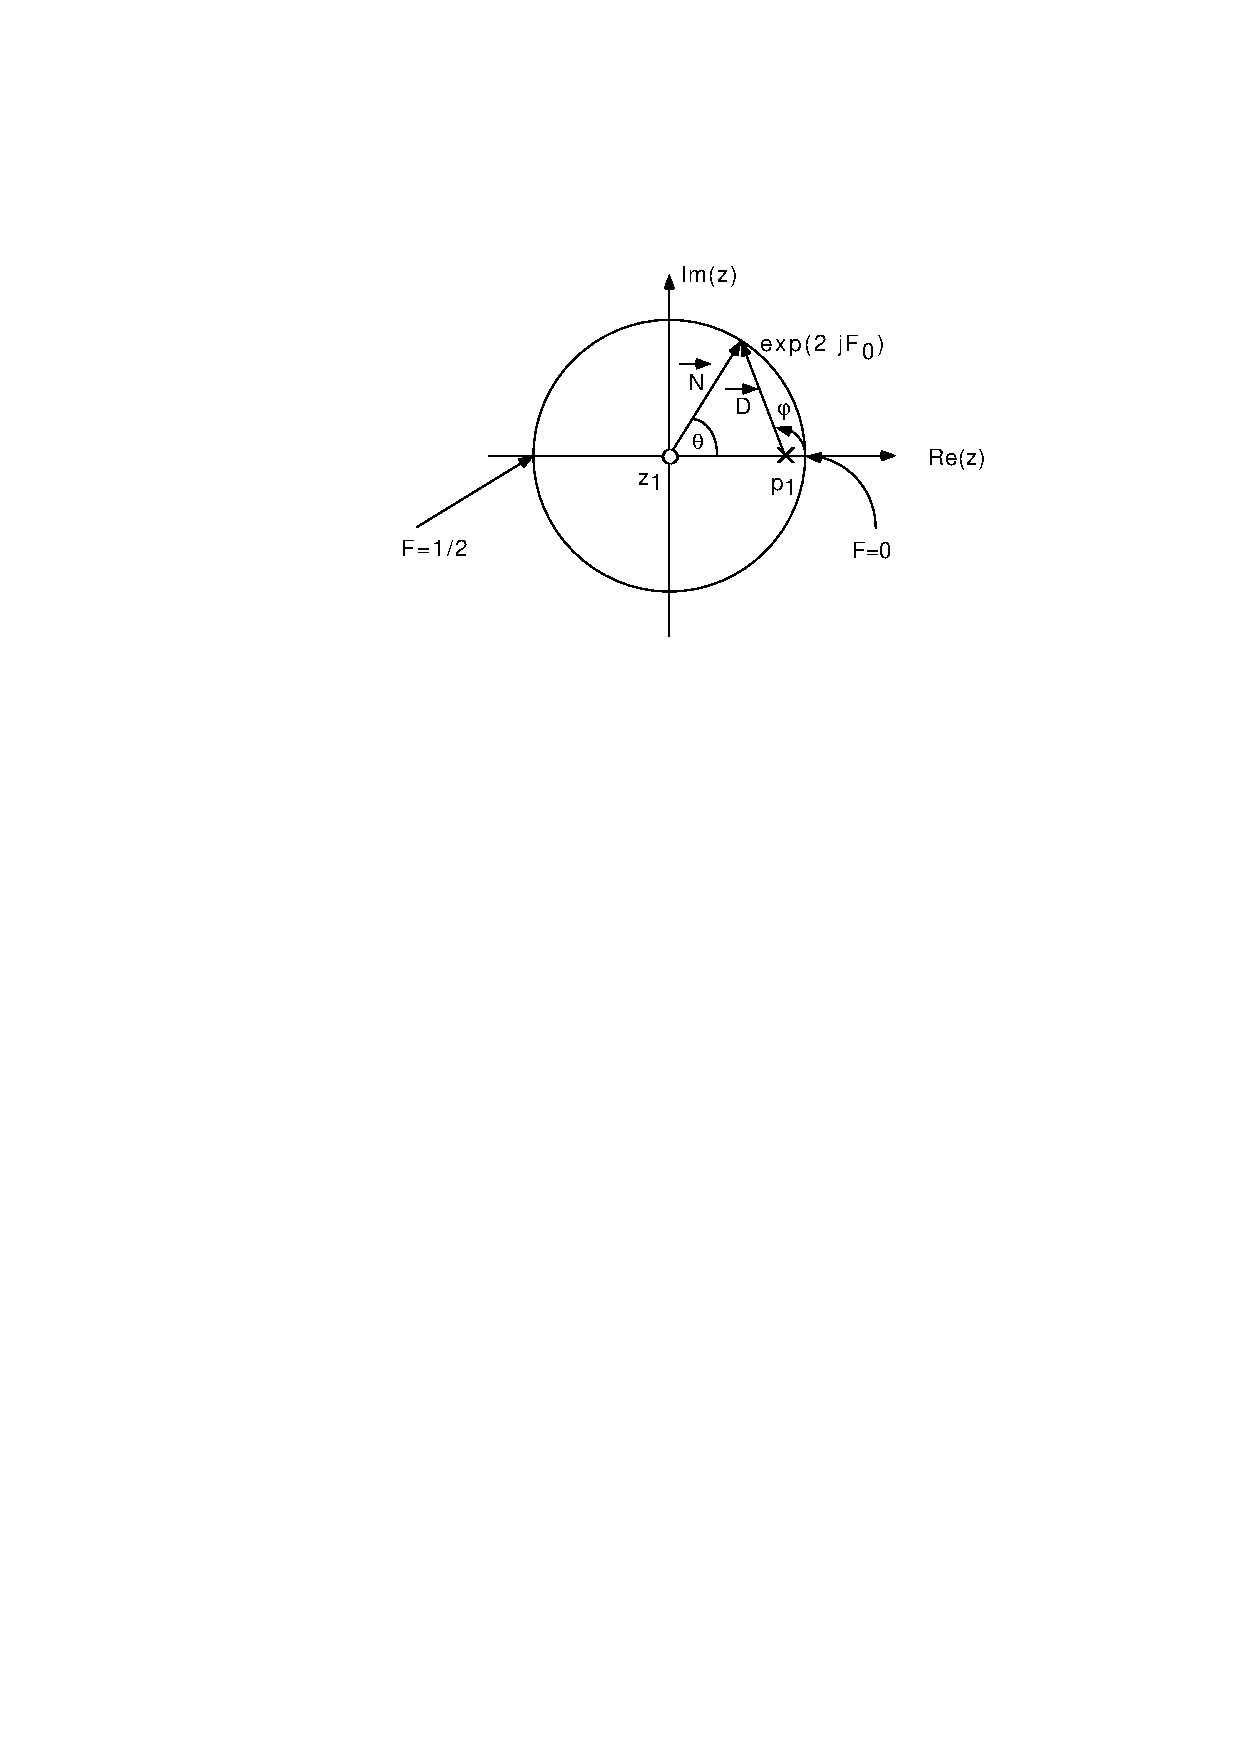
\includegraphics[width=0.6\textwidth]{Figures/FigMignotte-1}\\
  \caption{Réponse en fréquence de $z \mapsto U(z)= 1/(1-az^{-1})$}\label{fig:FigMignotte-1}
\end{figure}

Le calcul de la transform\'{e}e de Fourier requiert d'\'{e}valuer la transform\'{e}e en $z$ sur le cercle de rayon unit\'{e}. Pour une fr\'{e}quence
$\nu$, on pose $z=\cfoo$ et donc
$$
U(\cfoo)=\frac{\cfoo}{\rme^{\cfoo-a}}\
$$
Quand la fr\'{e}quence change, le module du num\'{e}rateur ne change pas. Par contre le module du d\'{e}nominateur d\'{e}cro\^{i}t lorsque l'on se rapproche d'un p\^{o}le. Plus pr\'{e}cis\'{e}ment, lorsque $2\pi \nu$ se rapproche de l'argument d'un p\^{o}le, le d\'{e}nominateur devient petit, et le module de la transform\'{e}e de Fourier devient grand.  Le module de la transform \'{e}e de Fourier prend donc des valeurs importantes pour des valeurs de pulsations proches de l'argument du  p\^{o}le. Cette
valeur sera d'autant plus \'{e}lev\'{e}e que le p\^{o}le a un module proche de l'unit\'{e}. On aurait pu tenir le m\^{e}me raisonnement avec les z\'{e}ros, qui occasionnent quant \`{a} eux des valeurs faibles (voire des z\'{e}ros de transmission) de la transform\'{e}e de Fourier.
Ici pour $\nu=0$, le module du d\'{e}nominateur a une certaine valeur. Ce module cro\^{i}t au fur et \`{a} mesure que l'on s'\'{e}loigne de cette fr\'{e}quence et atteint son maximum en $\nu=-1$.  Par ailleurs, le signal est ici r\'{e}el et on a en plus que le module de la transform\'{e}e de Fourier est pair, et l'argument, impair. Ces consid\'{e}rations sont illustr\'{e}es par la transform\'{e}e de Fourier donn\'{e}e \`{a} la \Cref{fig:FigMignotte-2} pour $a=0.9$.

Les consid\'{e}rations qui ont permis de pr\'{e}dire l'allure du spectre en module et argument peuvent aussi \^{e}tre utilis\'{e}es dans des situations plus compliqu\'{e}es. Consid\'{e}rant la transform\'{e}e en $z$ donn\'{e}e par \eqref{eq:transformee-z-generale}. Dans ce cas le module et l'argument sont donn\'{e}s par
\begin{align*}
|H\left(\rme^{2 \rmi \pi \nu}\right)|= \frac{\prod_{m=1}^N |1 -z_m \rme^{-2 \rmi \pi \nu}|}{\prod_{n=1}^N |1 - p_n \rme^{-2 \rmi \pi \nu}|} \\
\end{align*}
\begin{multline*}
H\left(\rme^{2 \rmi \pi \nu}\right)\ =\ \arg C+\sum_{m=1}^{M}\arg(\rme^{2 \rmi \pi \nu}-z_{m}) \\-
\sum_{m=1}^{N}\arg(\rme^{2 \rmi \pi \nu}-p_{n})
\end{multline*}

\begin{figure}
  \centering
  % Requires \usepackage{graphicx}
  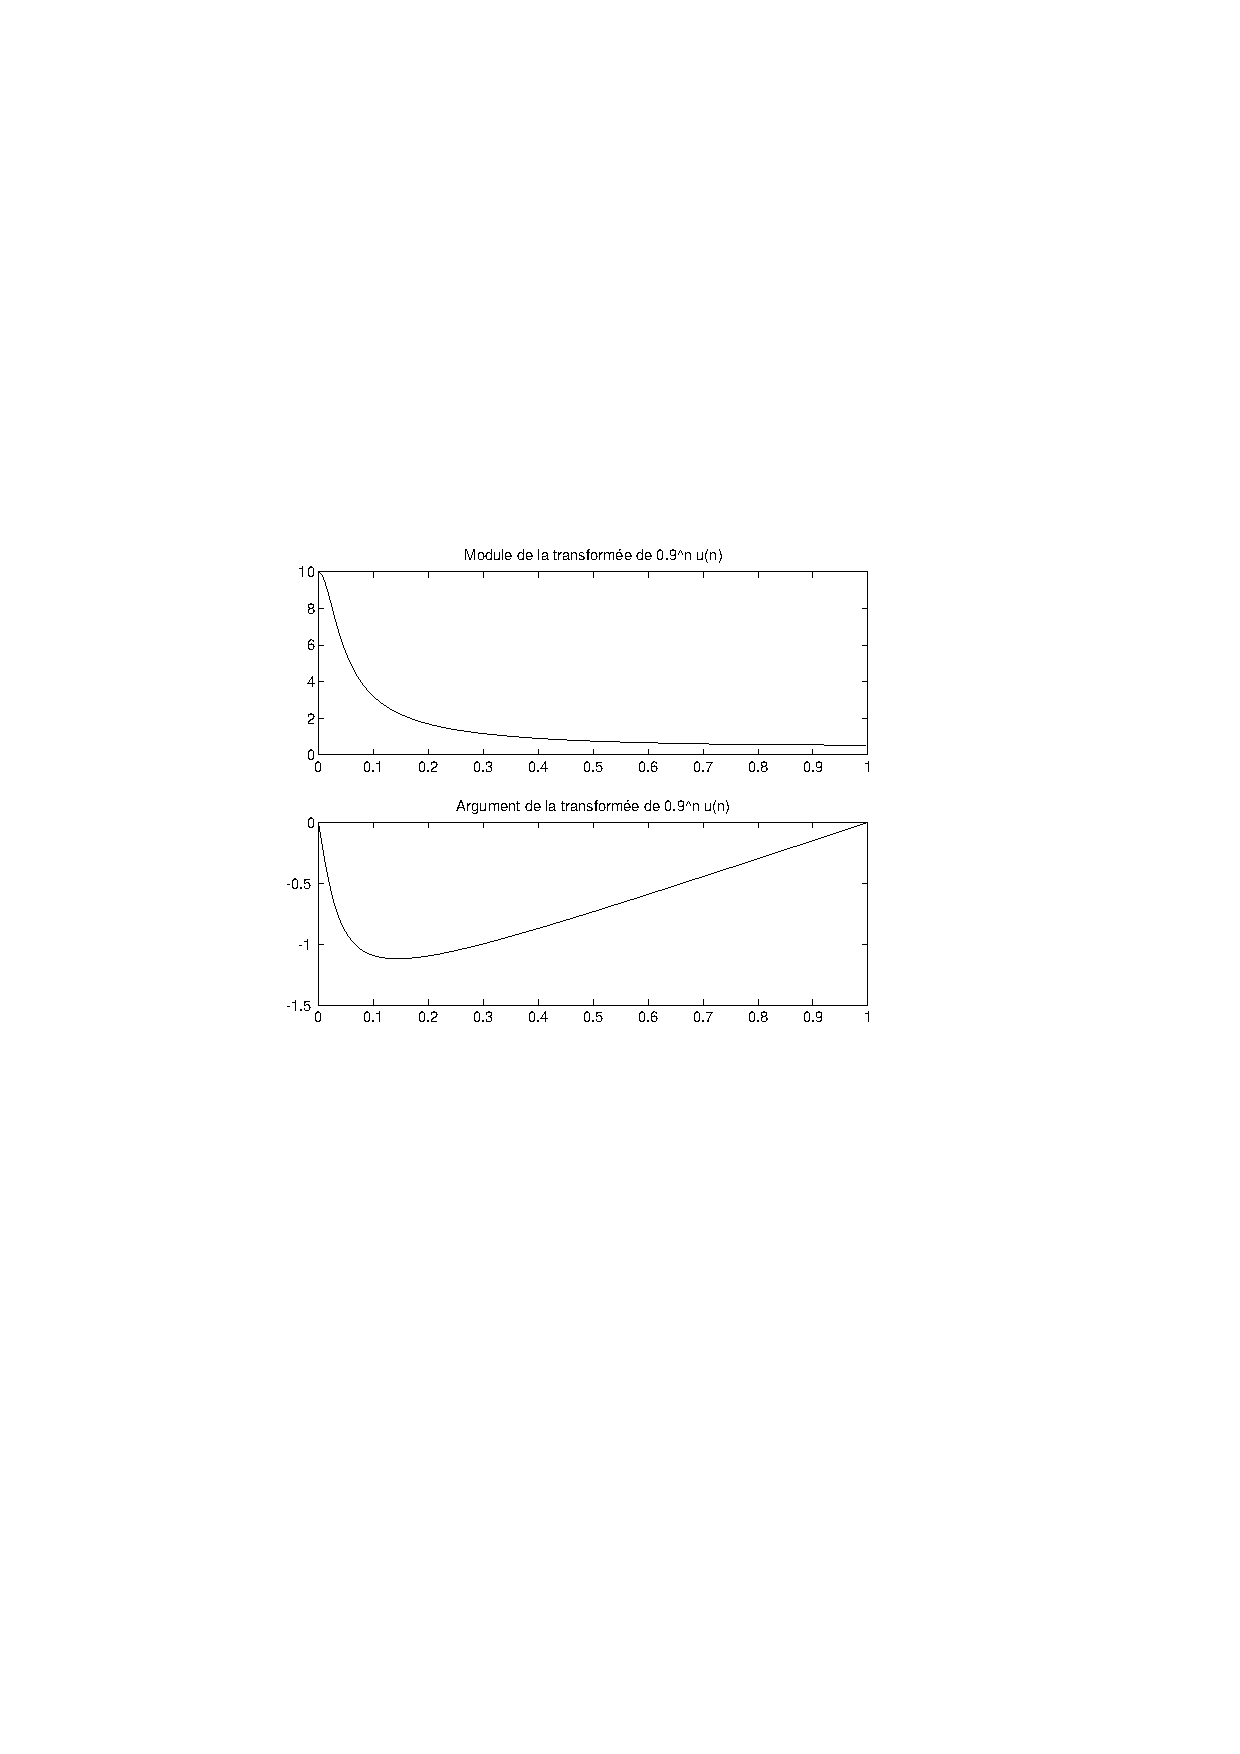
\includegraphics[width=0.6\textwidth]{Figures/FigMignotte-2}\\
  \caption{Transform\'{e}e de Fourier, module en haut, argument en bas, de $h_n= a^n \1_\nset(n)$ pour $a=0.9$
}\label{fig:FigMignotte-2}
\end{figure}
\section{Fonction de tranfert}
On a vu que la sortie $\sequence{v}[n][\nset]$ d'un système linéaire invariant dans le temps de r\'{e}ponse impulsionnelle $\sequence{h}[n][\nset]$ est donn\'{e}e par la convolution du signal d'entr\'{e}e $\sequence{u}[n][\nset]$ et de la réponse impulsionnelle $\sequence{h}[n][\nset]$, \ie\
$v_nj = (h * x)_n$ pour tout $n \in \zset$. La transformée en $z$ d'un produit de convolution étant égal au produit des transformées (la région de convergence étant l'intersection des régions de convergence de $U(z)$ et $H(z)$), nous avons donc
$$
V(z)=H(z)U(z) \eqsp.
$$
La transform\'{e}e en $z$, $H(z)$  de la r\'{e}ponse impulsionnelle $\sequence{h}[n][\zset]$ porte le nom de \emph{fonction de transfert} du syst\`{e}me lin\'{e}aire invariant. Cette transform\'{e}e en $z$, \'{e}valu\'{e}e sur le cercle de rayon unit\'{e} donne la transform\'{e}e de Fourier $H(\rme^{2 \rmi \pi \nu})$ de cette r\'{e}ponse impulsionnelle porte le nom de \emph{transmittance du syst\`{e}me} (on utilise aussi
fonction de transfert pour cette quantité, bien que cette terminologie soit un peu incorrecte).

\section{Causalité et Stabilité}
\begin{definition}[SLI causal]
On dit qu'un système linéaire invariant dans le temps est causal si $h_n=0$ pour $n < 0$ où $\sequence{h}[n][\zset]$ est sa réponse impulsionnelle
\end{definition}
On a vu que la région de convergence de la transform\'{e}e en $z$ d'une suite causale $\sequence{h}[n][\nset^]$
est une couronne  $\ensemble{z \in \cset}{|z| \geq \limsup_{n \to \infty} |h_n|^{1/n}= R_-}$. Comme par définition
une transform\'{e}e $H(p)= \infty$ lorsque $z= p$ est un pôle, une suite est causale si et seulement si
tous les p\^{o}les sont n\'{e}cessairement contenus \`{a} l'int\'{e}rieur d'un disque.

\begin{proposition}
la fonction de transfert d'un syst\`{e}me causal (c'est-\`{a}-dire dont la r\'{e}ponse impulsionnelle est causale) a ses p\^{o}les \`{a} l'int\'{e}rieur d'un cercle.
\end{proposition}

\begin{definition}[SLI stable]
un syst\`{e}me linéaire invariant dans le temps est stable si sa r\'{e}ponse impulsionnelle $\sequence{h}[n][\nset]$ est absolument sommable,
$$
\sum_{n=-\infty}^{\infty}|h_n|<\infty \eqsp.
$$
\end{definition}
Or,
$$
|H(z)|=|\sum_{n=-\infty}^{\infty}h_n z^{-n}|\leq\sum_{n=-\infty}^{\infty}|h_nz^{-n}|
$$
et sur le cercle de rayon unit\'{e},
$$
|H(\rme^{2 \rmi \pi \nu})|=|\sum_{n=-\infty}^{\infty} |h_n|
$$
et si le dernier terme est born\'{e}, cela signifie bien que la transform\'{e}e de Fourier à temps-discret existe.  Donc, pour que le syst\`{e}me soit stable, le cercle de rayon unit\'{e} doit être inclus dans la région de convergence de la fonction de transfert qui est un anneau en toute g\'{e}n\'{e}ralit\'{e}.

Pour qu'un syst\`{e}me soit causal et stable, il faut que le cercle de rayon unit\'{e} appartienne au domaine de convergence, qui pour réponse causale est la couronne $\ensemble{z \in \cset}{|z| \geq R_-}$. Compte tenu de ce qui a \'{e}t\'{e} dit pr\'{e}c\'{e}demment, les p\^{o}les du syst\`{e}me doivent donc \^{e}tre contenus dans un disque $\ensemble{z \in \cset}{|z| < R}$ avec $R < 1$.

\section{Equations aux diff\'{e}rences}
\subsection{fonction de transfert}
Lorsque le syst\`{e}me est r\'{e}gi par une \'{e}quation aux diff\'{e}rences du type
\begin{equation}
\label{eq:equation-aux-differences}
\sum_{l=0}^{N}a_{l}y_{n-l}=\sum_{m=0}^{M}b_{m}x_{n-m}
\end{equation}
o\`{u} $\sequence{x}[n][\zset]$ et $\sequence{y}[n][\zset]$ sont les suites d'entr\'{e}e (excitation) et de sortie (r\'{e}ponse), on peut obtenir la r\'{e}ponse de r\'{e}gime en passant par la transform\'{e}e en $z$ bilat\'{e}rale. En utilisant les propri\'{e}t\'{e}s de lin\'{e}arit\'{e} et d\'{e}calage, on trouve finalement
\begin{equation}
\label{eq:tz-equation-difference}
Y(z)\sum_{l=0}^{N}a_{l}z^{-l}=X(z)\sum_{m=0}^{M}b_{m}z^{-m}
\end{equation}
On en d\'{e}duit que la fonction de transfert $G(z)$
$$
G(z)=\frac{\sum^{M}b_{m}z^{-m}}{\sum_{l=0}^L a_{l}z^{-l}} \eqsp
$$
est une fraction rationnelle (en $z^{-1}$). Il est souvent pratique de factoriser les polynômes apparaissant
au numérateur et au dénominateur, \ie\ d'écrire
$$
G(z)= \frac{b_0}{a_0} \frac{\prod_{k=1}^M (1-c_k z^{-1})}{\prod_{l=1}^N (1-d_k z^{-1})}
$$
Chaque facteur au numérateur $(1-c_k z^{-1})$ sont associés à un zéro en $z= c_k$ et un pôle en $z=0$.
Chaque facteur au dénominateur est  associé à un pôle en $z=d_k$
et un zéro en  $z=0$.
\subsection{causalité et stabilité}
Pour obtenir \eqref{eq:tz-equation-difference} à partir de \eqref{eq:equation-aux-differences}, nous avons supposé que \eqref{eq:equation-aux-differences} représentait un système linéaire invariant dans le temps, mais nous n'avons pas fait d'hypothèses supplémentaires sur la stabilité ou la causalité du système. Pour spécifier réellement la relation d'entrée-sortie associée à \eqref{eq:equation-aux-differences}, il est maintenant important de considérer précisément les domaines de convergence, car comme nous le verrons \eqref{eq:equation-aux-differences} ne spécifie pas une unique relation de filtrage mais un ensemble de relations de filtrages, associées à la fois aux différents domaines de convergence de la fonction de transfert $G(z)$ et du domaine de convergence de l'entrée $X(z)$. Pour une fraction rarionnelle, chaque choix de la région de convergence sera associé à une réponse impulsionnelle différente, bien qu'étant associée à la \emph{même} équation aux différences. Une certaine prudence s'impose donc !
Supposons que $M < N$ et que les pôles sont simples. Dans ce cas $G(z)$ peut se développer de la façon suivante
\[
G(z)= \sum_{k=1}^N \frac{A_k}{1 - d_k z^{-1}} \eqsp,
\]
où $A_k= (1-d_k z^{-1}) A(z)\vert_{z=d_k}$.  Lorsque $M > N$, on doit tout d'abord procéder à la division euclidienne du numérateur par le dénominateur, puis on applique le résultat précédent au reste de cette division euclidienne
\[
G(z)= \sum_{r=0}^{M-N} B_r z^{-r} + \sum_{k=1}^N \frac{A_k}{1-d_k z^{-1}} \eqsp.
\]
Pour obtenir les solutions causales, nous développons
\[
\frac{1}{1-d_k z^{-1}} = \sum_{j=0}^{\infty} d_k^j z^{-j} \eqsp,
\]
qui converge sur la couronne $\ensemble{z \in \cset}{|d_k| \leq |z|}$. Le domaine de convergence de la solution causale est donc $R_- = \max ( |d_k|, k \in \{1,\dots,N\})$ et la réponse associée est donc
\[
G(z)= \sum_{r=0}^{M-N} B_r z^{-r} + \sum_{k=1}^N A_k \sum_{j=0}^{\infty} d_k^j z^{-j} \eqsp.
\]
La réponse impusionnelle est stable si le cercle unité est élément de la région de convergence, ce qui implique que tous les pôles sont \emph{à l'intérieur du disque unité} (dans ce cas, $R_- < 1$).

Si cette condition n'est pas satisfaite, il peut néanmoins exister une réponse stable. Supposons que $A(z) \ne 0$ pour $|z|=1$ (le système n'a pas de pôles sur le cercle unité). Nous utilisons les développements suivants
\begin{equation}
\label{eq:developpement-pole}
\begin{cases}
|d_k| < 1 & \frac{1}{1-d_k z^{-1}}= \sum_{j=0}^\infty d_k^j z^{-j} \\
 \mathrm{DC} \quad \ensemble{ z \in \cset}{|d_k| \leq |z|} \\
|d_k| > 1 & \frac{1}{1-d_k z^{-1}}= - \frac{d_k^{-1} z}{1 - d_k^{-1} z} = - \sum_{j=1}^\infty d_k^j z^{-j} \\
 \mathrm{DC} \quad \ensemble{z \in \cset}{|z| < |d_k|}
\end{cases}
\end{equation}
Le domaine de convergence est alors une couronne $R_- = \max \{ |d_k| < 1, k \in \{1, \dots, N\} \}$ et $R_+= \min \{ |d_k| > 1, k \in \{1, \dots, N\} \}$.
\begin{example}
Considérons la fonction de transfert
\[
G(z)= \frac{1-az^{-1}}{1-bz^{-1}} .
\]
Supposons que $|a| < 1$ et $|b| < 1$. La fonction de transfert a un zéro en $z=a$ et un pôle en $z=b$. Ce pôle est élément du disque unité ouvert et cette fonction de transfert admet donc un développement causal stable. Nous avons en effet
\[
\frac{1-az^{-1}}{1-bz^{-1}} = c + \frac{1-c}{1-b z^{-1}} \eqsp, \quad c= a/b \eqsp.
\]
Cette fraction rationelle admet un développement causal stable sur la couronne $\ensemble{z \in \cset}{|b| \leq |z|}$:
\[
G(z) = c + (1-c) \sum_{j=0}^\infty b^j z^{-j} \eqsp.
\]
On peut chercher à inverser ce système, c'est à dire trouver la fonction de transfert $G_1(z)$ qui soit telle que $G(z) G_1(z)= 1$.
Nous avons alors
\[
G_1(z)= \frac{1-bz^{-1}}{1-a z^{-1}}
\]
Cette fonction de transfert admet un pôle en $a$ et comme $|a| < 1$, la fonction de transfert inverse admet aussi un développement causal stable.
\end{example}
\begin{example}[filtre passe-tout]
Considérons le filtre de fonction de transfert
\[
G(z)= \frac{z^{-1} - \bar{a}}{1-a z^{-1}} \eqsp, \quad |a| \ne 1
\]
On remarque que le module de la réponse en fréquence de ce filtre est constant, \ie\
\[
G(\cfoo)= \frac{\foo - \bar{a}}{1 - a \foo}= \foo \frac{1 - \bar{a} \cfoo}{1 - a \foo} \eqsp,
\]
ce qui implique que $|G(\cfoo)|= 1$ pour tout $\nu \in \toref$. Un tel système est appelé un "passe-tout". De façon générale, la fonction de transfert d'un filtre passe-tout est donnée par
\[
G(z)= \prod_{k=1}^M \frac{z^{-1} - d_k}{1 - d_k z^{-1}} \prod_{k=1}^M \frac{(z^{-1} - \bar{e}_k)(z^{-1}-e_k)}{(1-e_k z^{-1})(1-\bar{e}_k z^{-1})} \eqsp,
\]
où $d_k$, $k \in \{1,\dots,M\}$ sont les pôles réels et $e_k$, $k \in \{1,\dots,M\}$ sont les pôles complexes.

\begin{figure}
  \centering
  % Requires \usepackage{graphicx}
  \begin{tabular}{cc}
  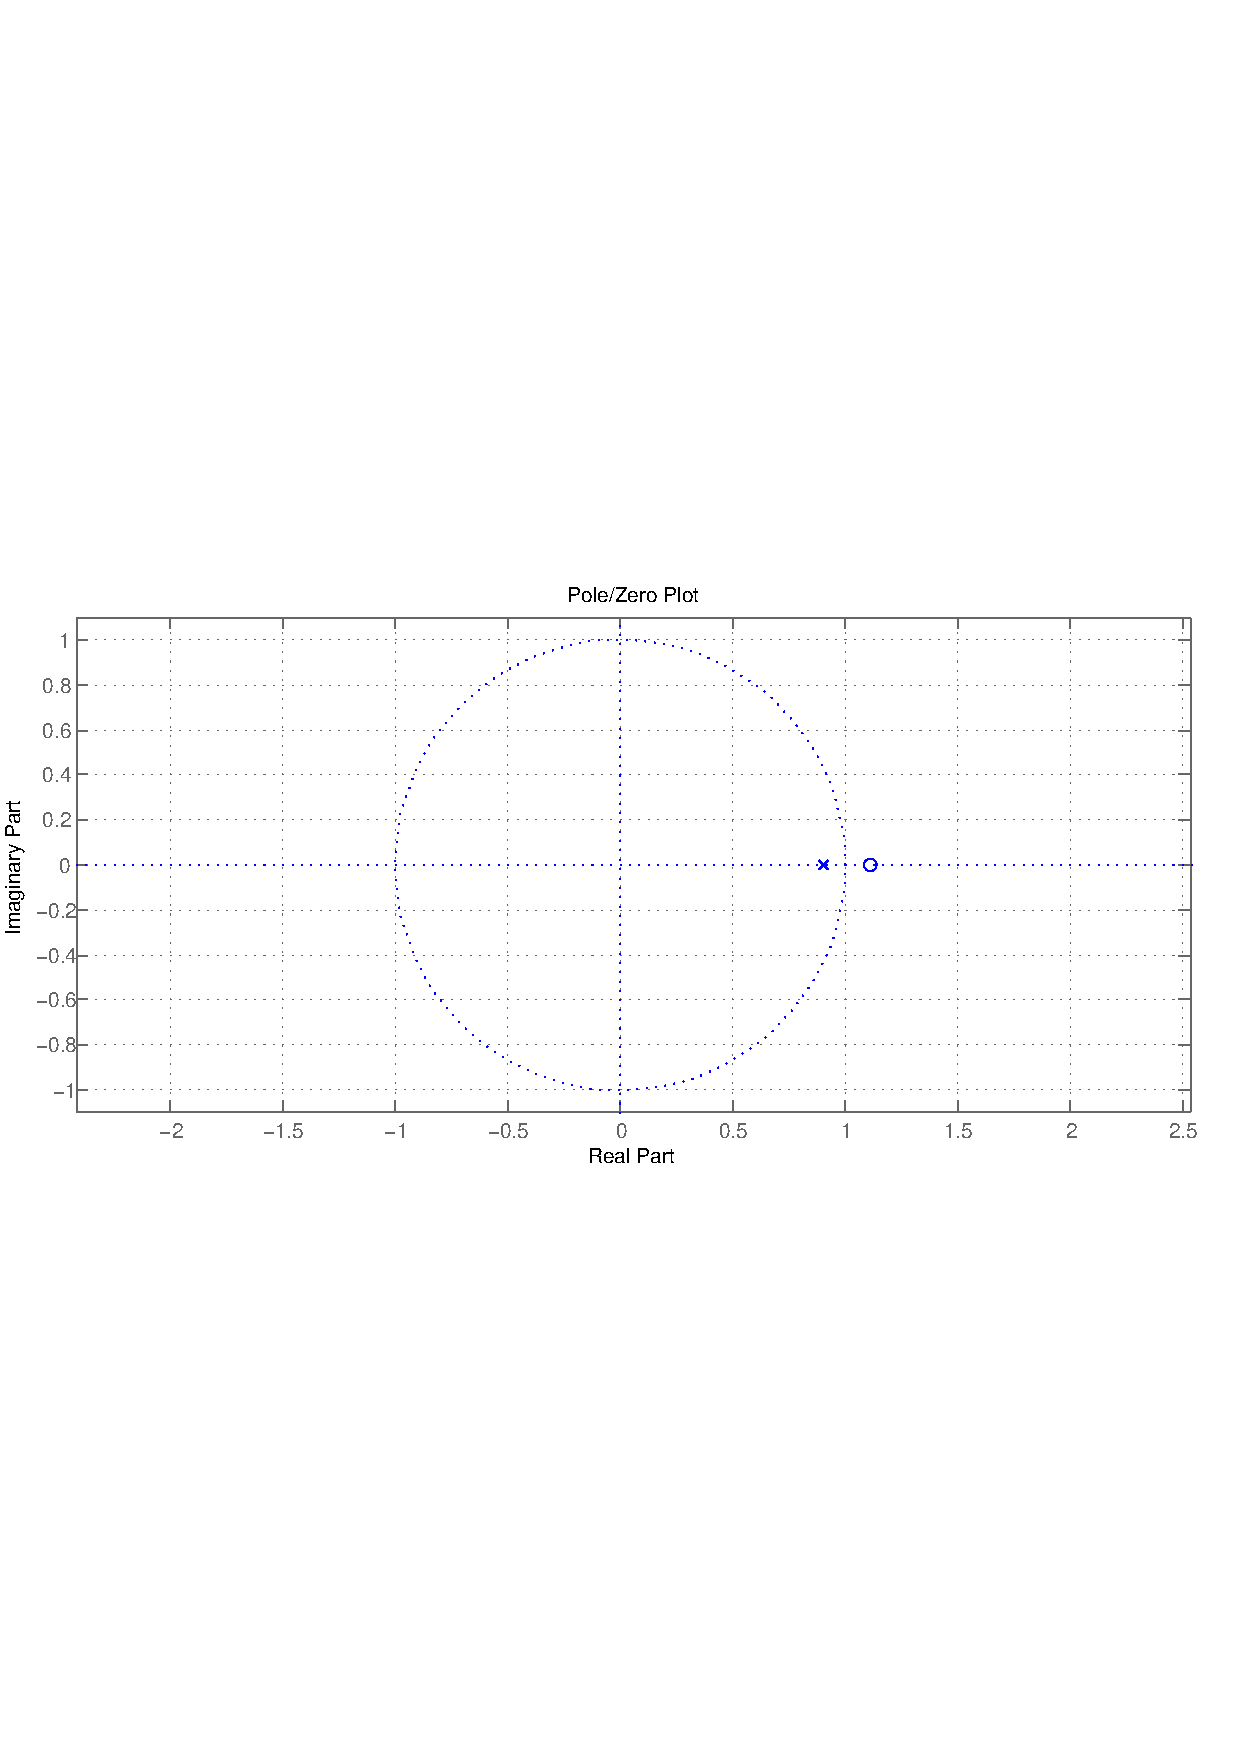
\includegraphics[width=0.4\textwidth]{Figures/polezero}& 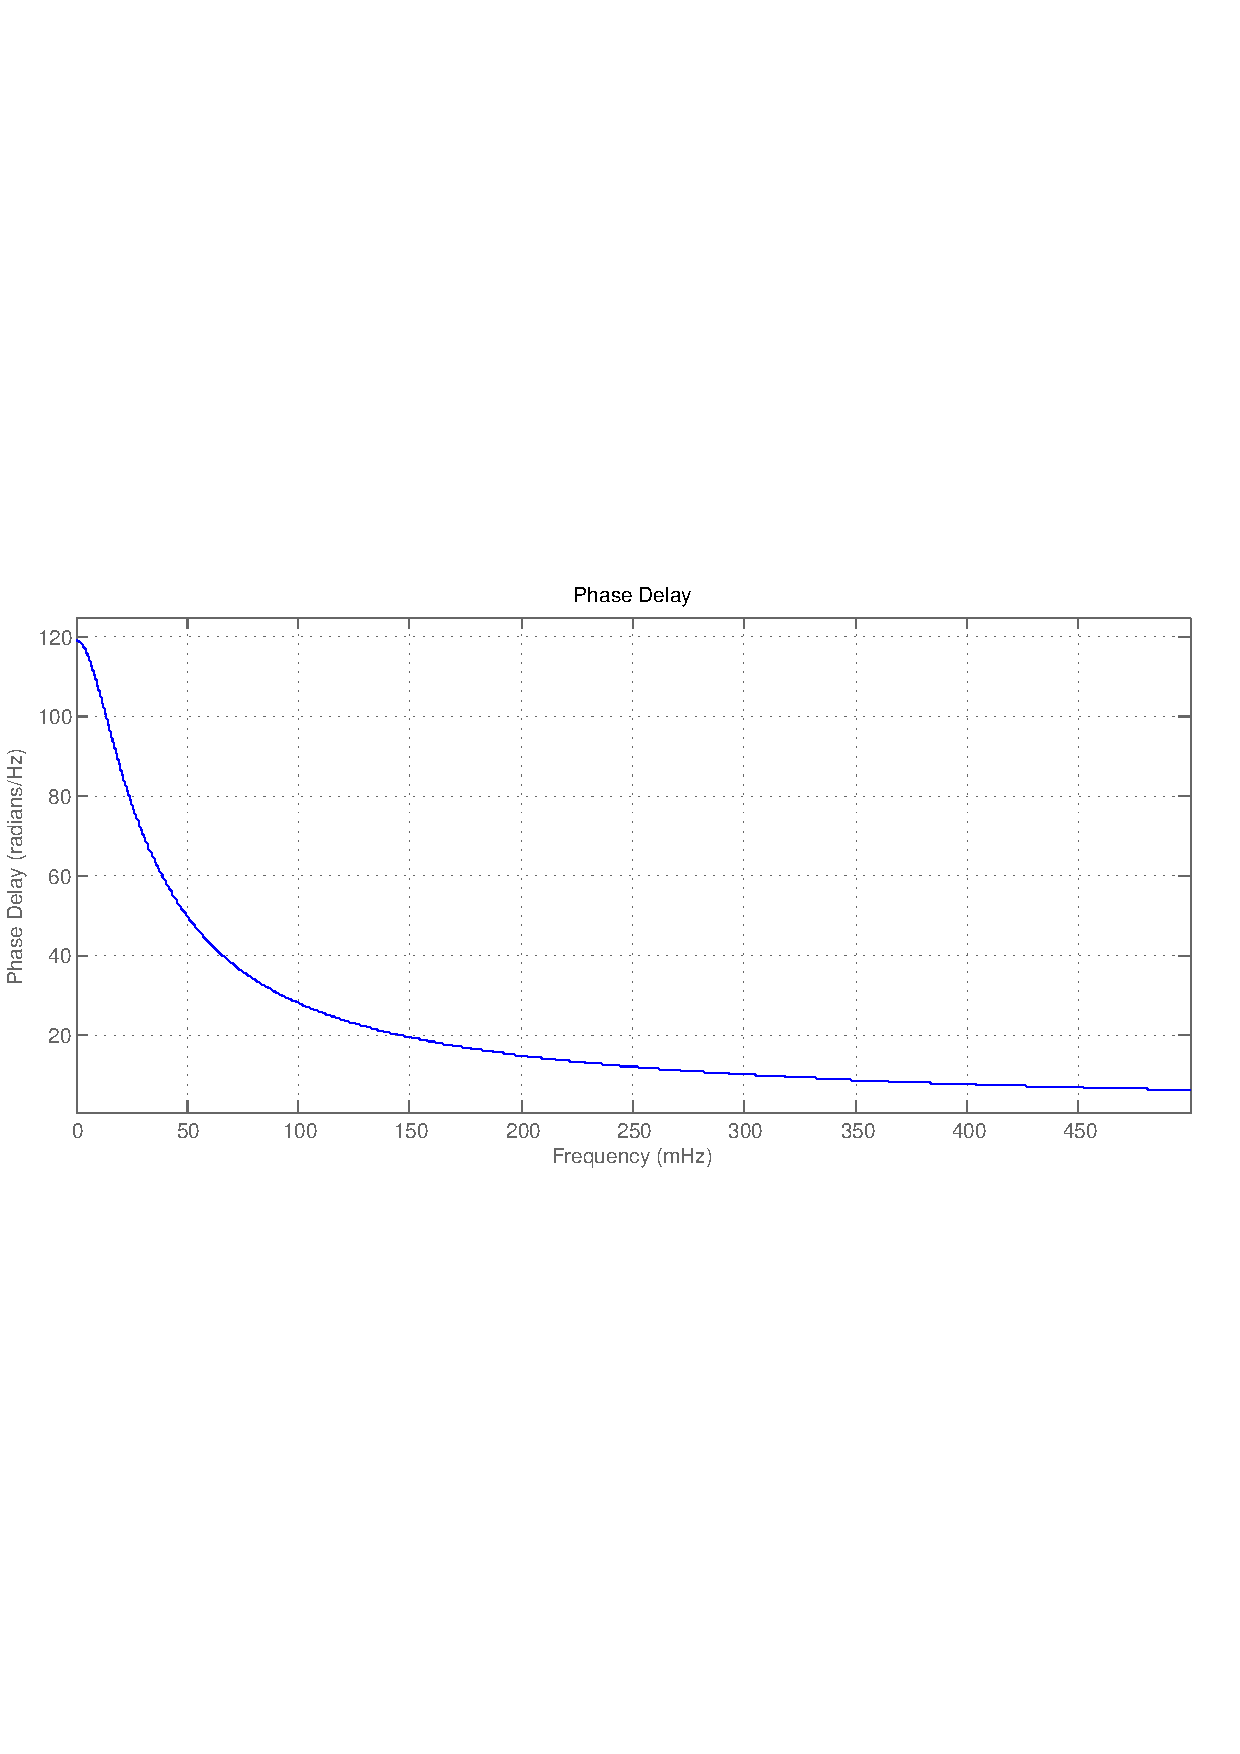
\includegraphics[width=0.4\textwidth]{Figures/phasedelay1}
    \end{tabular}
  \caption{Pôles et zéros et phase d'un filtre passe tout du premier ordre avec $a=0.9$}
  \label{fig:passetout-1}
\end{figure}


\end{example}

\begin{example}[Filtre de Karplus-Strong]

\end{example} 
\part{Bases de traitement du signal al\'eatoire}
\chapter{Introduction au signal al\'eatoire \`a temps-discret}

Dans ce chapitre, nous introduisons des concepts de base concernant
l'analyse des s\'eries temporelles. En particulier, nous d\'efinissons
les notions de stationnarit\'e et de fonction d'autocovariance.

\section{Introduction}

%% Nous commen\c{c}ons par d\'efinir ce qu'est une s\'erie temporelle.
%
%\index{S\'erie temporelle}\index{S\'erie chronologique|see{S\'erie temporelle}}
%Une s\'erie temporelle (ou s\'erie chronologique) est un ensemble
%d'observations $x_t$, chacune \'etant enregistr\'ee \`a un instant $t$.
%On rencontre des s\'eries temporelles dans des domaines tr\`es
%vari\'es tels que la m\'edecine, les t\'el\'ecommunications ou l'\'econom\'etrie.

% Notre but, dans cet ouvrage, est de proposer des m\'ethodes permettant
% de mod\'eliser de telles donn\'ees en utilisant un mod\`ele
% math\'ematique appropri\'e afin de pouvoir, par la suite, faire de la
% pr\'ediction. Pour cela, nous proposerons des m\'ethodes permettant
% d'estimer les param\`etres du mod\`ele choisi ainsi que des m\'ethodes
% permettant de tester la validit\'e du mod\`ele propos\'e.


%\paragraph{Exemples de s\'eries temporelles}
% Le paragraphe~\ref{sec:gene} d\'efinit le formalisme probabiliste
% permettant de d\'ecrire les {\em processus al\'eatoires}. Les quelques
% exemples qui suivent illustrent la diversit\'e des situations dans
% lesquelles la mod\'elisation stochastique (ou al\'eatoire) des s\'eries
% temporelles joue un r\^ole important.

Dans la suite, nous proposons de consid\'erer les observations comme
des r\'ealisations d'un processus al\'eatoire $(X_t)_{t\in T}$ dont nous
donnons la d\'efinition dans le paragraphe \ref{sec:gene}. Les quelques
exemples qui suivent illustrent la diversit\'e des situations dans
lesquelles la mod\'elisation stochastique (ou al\'eatoire) des s\'eries
temporelles joue un r\^ole important.
\begin{example}[Trafic internet]
La figure \ref{fig:figtraf} repr\'esente les temps d'inter-arriv\'ees
de paquets TCP, mesur\'es en secondes, sur la passerelle du
laboratoire Lawrence Livermore. La trace repr\'esent\'ee a \'et\'e obtenue
en enregistrant 2 heures de trafic. Pendant cette dur\'ee, environ
1.3 millions de paquets TCP, UDP, etc. ont \'et\'e enregistr\'es, en
utilisant la proc\'edure \emph{tcpdump} sur une station Sun.
D'autres s\'eries de ce type peuvent \^{e}tre obtenues sur
\emph{The Internet Traffic Archive},
\emph{http://ita.ee.lbl.gov/}.
%======== FIGURE
\begin{figure}
  \centering
  % Requires \usepackage{graphicx}
  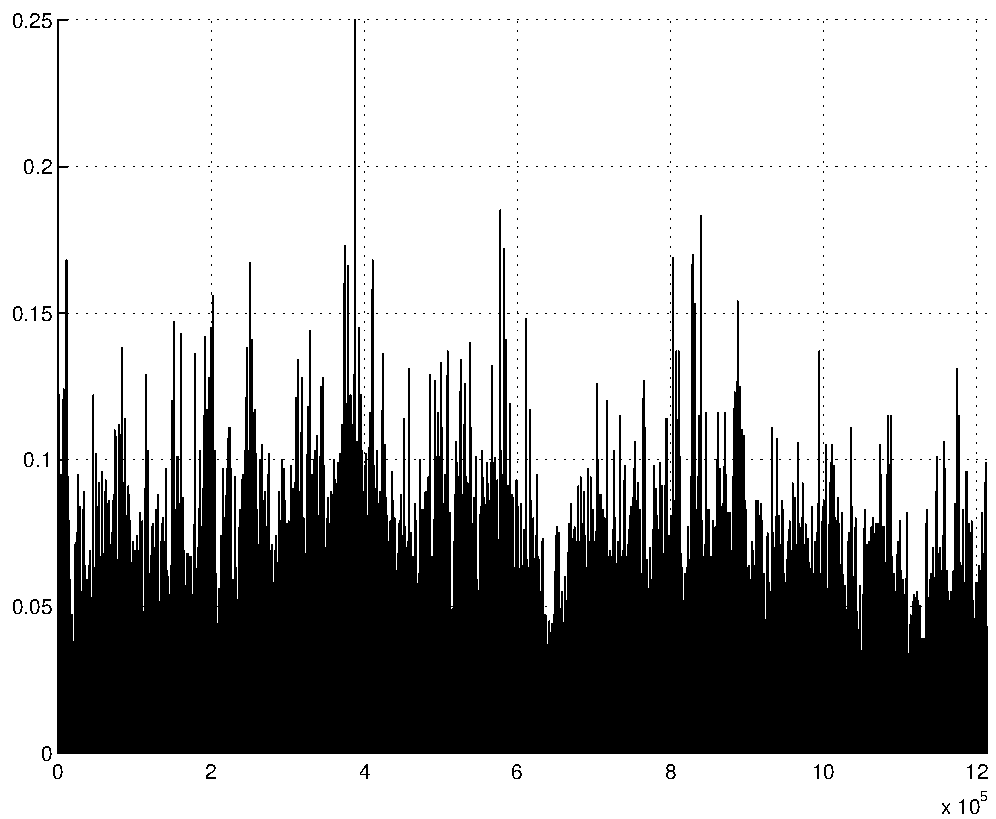
\includegraphics[width=\textwidth]{Figures/lbl_tcp_3}\\
  \caption{Trace de trafic Internet~: temps d'inter-arriv\'ees de paquets TCP.}\label{fig:figtraf}
\end{figure}
\end{example}
\begin{example}[Parole]
La figure \ref{fig:figspeech} repr\'esente un segment de signal
vocal \'echantillonn\'e (la fr\'equence d'\'echantillonnage est de 8000
Hz). Ce segment de signal correspond \`a la r\'ealisation du
phon\`eme \emph{ch} (comme dans \emph{ch}at) qui est un son
dit \emph{fricatif}, c'est-\`a-dire produit par les turbulences du
flot d'air au voisinage d'une constriction (ou resserrement) du
conduit vocal.
%======== FIGURE
\begin{figure}
  \centering
  % Requires \usepackage{graphicx}
  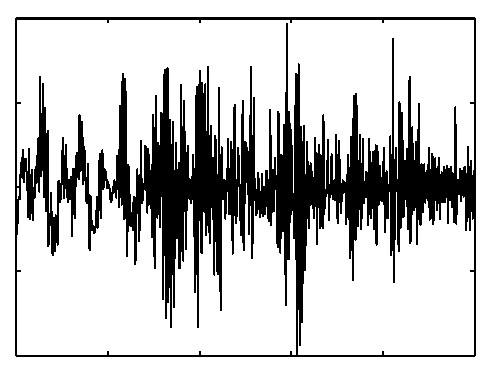
\includegraphics[width=\textwidth]{Figures/phrase}\\
  \caption{Signal de parole \'echantillonn\'e \`a $8000$ Hz~:
 son non vois\'e \emph{ch}.}\label{fig:figspeech}
\end{figure}
\end{example}

\begin{example}[Indice financier]
La figure~\ref{fig:SP} repr\'esente les cours d'ouverture
journaliers de l'indice Standard and Poor 500, du $2$ Janvier
$1990$ au 25 Ao\^ut 2000. l'indice S\&P$500$ est calcul\'e \`a
partir de $500$ actions choisies parmi les valeurs cot\'ees au New
York Stock Exchange (NYSE) et au NASDAQ en fonction de leur
capitalisation, leur liquidit\'e, leur repr\'esentativit\'e dans
diff\'erents secteurs d'activit\'e. Cet indice est obtenu en pond\'erant
le prix des actions par le nombre total d'actions, le poids de
chaque valeur dans l'indice composite \'etant proportionnel \`a la
capitalisation.
%======== FIGURE
\begin{figure}
  \centering
  % Requires \usepackage{graphicx}
  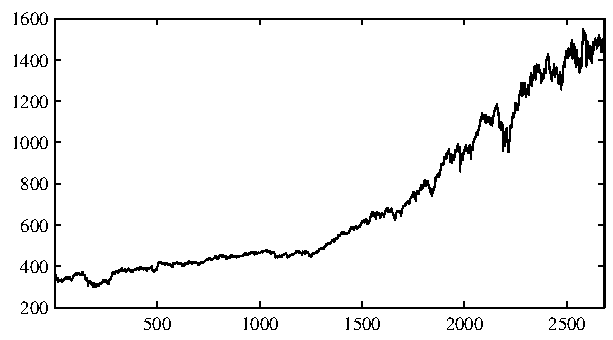
\includegraphics[width=\textwidth]{Figures/SP}\\
  \caption{Cours quotidien d'ouverture de l'indice S\&P$500$~:
 entre Janvier 1990 et Ao\^ut 2000.}\label{fig:SP}
\end{figure}
\end{example}


\section{D\'efinition et construction de la loi d'un processus al\'eatoire}
\label{sec:gene}
%=================================================================
\subsection{Processus al\'eatoire}

\begin{definition}[Processus al\'eatoire]
\index{Processus!Al\'eatoire}
Soient $(\Omega,\cF,\PP)$ un espace de probabilit\'e, $T$ un
ensemble d'indices et $(E,\cE)$ un espace mesurable. On appelle
processus al\'eatoire une famille $(X_t)_{t \in T}$ de v.a. \`a
valeurs dans $(E,\cE)$ index\'ees par $t \in T$.
\end{definition}
Le param\`etre $t$ repr\'esente par exemple le temps. Lorsque $T=
\Zset$ ou $\Nset$, nous dirons que le processus est \`a \emph{temps discret}
et, lorsque $T=\Rset$ ou $\Rset_+$, que le processus est \`a
\emph{temps continu}. Dans la suite, nous nous
int\'eresserons sauf exception aux processus \`a temps
discret avec $T= \Zset$. Quant \`a $(E,\cE)$, nous consid\`ererons
le plus souvent $(\Rset, \cB(\Rset))$ (o\`u $\cB(\Rset)$ est la
tribu bor\'elienne de $\Rset$) ou $(\Rset^d, \cB(\Rset^d))$.
Dans le premier cas, on dira que le processus al\'eatoire est
\emph{scalaire}. Dans le second, nous dirons que le processus est
\emph{vectoriel}.

Notons qu'un processus peut \^{e}tre vu comme une application $X: \Omega
\times T \rightarrow E$, $(\omega,t)\mapsto X_t(\omega)$ telle que, \`a
chaque instant $t \in T$, l'application $\omega \mapsto X_t(\omega)$
est une variable al\'eatoire de $(E,\cE)$.
\begin{definition}[Trajectoire\index{Trajectoire}]
  Pour chaque $\omega\in \Omega$, l'application $t \mapsto
  X_t(\omega)$ est une fonction de $T \rightarrow E$ qui s'appelle la
  \emph{trajectoire} associ\'ee \`a l'\'epreuve $\omega$.
\end{definition}

%==================================================
%==================================================
\subsection{R\'epartitions finies}
%==================================================

Etant donn\'es 2 espaces mesurables $(E_1,\cE_1)$ et $(E_2,\cE_2)$, on d\'efinit l'espace mesurable produit
$(E_1\times E_2,\cE_1\otimes\cE_2)$ o\`u $\times$ d\'esigne le produit cart\'esien usuel des ensembles
et $\otimes$ l'op\'eration correspondante sur les tribus: $\cE_1\otimes\cE_2$ d\'esigne la tribu engendr\'ee par $\{A_1\times A_2,
A_1\in\cE_1: A_2\in\cE_2\}$, ce que l'on \'ecrira
$$
\cE_1\otimes\cE_2=\sigma\{A_1\times A_2: A_1\in\cE_1, A_2\in\cE_2\} \; .
$$
Comme la classe d'ensembles $\{A_1\times A_2: A_1\in\cE_1,
A_2\in\cE_2\}$ est stable par intersection finie, une probabilit\'e sur
$\cE_1\otimes\cE_2$  est \emph{caract\'eris\'ee} par sa restriction \`a
cette classe (voir \cite[Corollaire 6.1]{jacod:protter:2003}).

On d\'efinit de m\^{e}me un espace mesurable produit $(E_1\times\dots\times E_n,\cE_1\otimes\dots\otimes\cE_n)$
\`a partir d'un nombre fini $n$ d'espaces mesurables $(E_t,\cE_t)$,
$t\in T$. Si $T$ n'est pas de cardinal fini, cette d\'efinition se g\'en\'eralise en consid\'erant
 la tribu engendr\'ee par les \emph{cylindres} sur le produit cart\'esien $\prod_{t\in T} E_t$ qui contient l'ensemble des
 familles $(x_t)_{t\in T}$ telles que $x_t\in E_t$ pour tout $t\in T$. Examinons le cas qui nous servira par la suite o\`u
$(E_t,\cE_t)=(E,\cE)$ pour tout $t\in T$. On note alors $E^T=\prod_{t\in T} E$ l'ensemble des trajectoires $(x_t)_{t\in T}$
telles que $x_t\in E$ pour tout $t$, que l'on munit de la tribu engendr\'ee par les cylindres
$$
\cE^{\otimes T}=\sigma\left\{\prod_{t\in I}A_{t}\times E^{T\setminus I} : I\in\mathcal{I},\forall t\in I,\,A_t\in\cE\right\}\;,
$$
o\`u l'on note $\mathcal{I}$ l'ensemble des parties finies de $T$.



%Un \'el\'ement $I$ de $\mathcal{I}$ s'\'ecrit $I = \{ t_1 < t_2 <\cdots < t_n \}$.
Soit $X=(X_t)_{t \in T}$ un processus d\'efini sur  $(\Omega,\cF,\PP)$ \`a
valeurs dans $(E,\cE)$  et $I\in\mathcal{I}$.
On note $\PP_I$ la loi du vecteur al\'eatoire $\{ X_{t}, {t\in I} \}$, c'est-\`a-dire la mesure image  de $\PP$ par ce vecteur~: $\PP_I$ est
la probabilit\'e sur $(E^{I},\cE^{\otimes I})$ d\'efinie par
\begin{equation}
\label{eq:rel1}
\PP_I\left(\prod_{t\in I}A_t\right)
 = \PP\left(X_{t} \in A_t,\,t\in I\right) \eqsp,
\end{equation}
o\`u $A_t$, $t\in T$ sont des \'el\'ements quelconques de la tribu $\cE$. La probabilit\'e $\PP_I$ est
une \emph{probabilit\'e fini-dimensionnelle} ou \emph{r\'epartition finie} du processus $X$.
\begin{definition}
\index{Famille des r\'epartitions finies}
On appelle \emph{famille des r\'epartitions finies} l'ensemble des
r\'epartitions finies $(\PP_I, I \in \mathcal{I})$.
\end{definition}
La sp\'ecification de la mesure $\PP_I$ permet de calculer la
probabilit\'e d'\'ev\'enements de la forme $\PP( \cap_{t \in I} \{
X_t \in A_t \})$ o\`u $\{A_t, t \in I\}$ est une famille d'\'el\'ements de la
tribu $\cE$, ou de mani\`ere \'equivalente, de calculer l'esp\'erance
$\PE {\prod_{t \in I} f_t(X_t) }$ o\`u pour tout $t\in I$, $f_t$ est une
fonction bor\'elienne positive. Soit
$J \subset I$ deux parties finies ordonn\'ees. Soit $\Pi_{I,J}$ la
projection canonique de $E^{I}$ sur $E^{J}$ d\'efinie par
\begin{equation}
\label{eq:rel2} \Pi_{I,J}[ x ] = (x_t)_{t \in J}\quad \text{pour tout}\quad x=(x_t)_{t \in I} \in E^I\;.
\end{equation}
La projection canonique pr\'eserve uniquement les coordonn\'ees du
vecteur appartenant au sous ensemble d'indices $J$.
Par la d\'efinition~(\ref{eq:rel1}), on observe que $\PP_J$ est la mesure image de $\Pi_{I,J}$ d\'efinie sur
l'espace de probabilit\'e $(E^{I},\cE^{\otimes I},\PP_I)$:
\begin{equation}
\label{eq:rel3} \PP_I \circ \Pi_{I,J}^{-1} = \PP_J \;.
\end{equation}
Cette relation
formalise le r\'esultat intuitif que la distribution
fini-dimensionnelle d'un sous-ensemble $J \subset I$ se d\'eduit de
la distribution fini-dimensionnelle $P_I$ en ``int\'egrant'' par rapport aux
variables $X_{t}$ sur l'ensemble des $t$ appartenant au
compl\'ementaire de $J$ dans $I$. Cette propri\'et\'e montre que la
famille des r\'epartitions finies d'un processus est fortement
structur\'ee. En particulier, les r\'epartitions finies doivent, au
moins, v\'erifier les conditions de compatibilit\'e~(\ref{eq:rel3}).
Nous allons voir dans la suite que cette condition est en fait
aussi {\em suffisante}.


Soit $\Pi_I$ la projection canonique de $E^T$ sur $E^I$,
\begin{equation}
\label{eq:projectioncanonique}
\Pi_I( x ) = (x_t)_{t \in I}\quad \text{pour tout}\quad x=(x_t)_{t \in T} \in E^T\;.
\end{equation}
Si $I=\{s\}$ avec $s\in T$, on notera simplement
\begin{equation}
\label{eq:projectioncanoniquesingle}
\Pi_s( x ) =\Pi_{\{s\}}( x )= x_s\quad \text{pour tout}\quad x=(x_t)_{t \in T} \in E^T\;.
\end{equation}

Le th\'eor\`eme suivant montre comment on peut passer d'une famille de
r\'epartitions finies \`a une unique mesure de probabilit\'e sur $(E^T,\cE^{\otimes
  T})$, pourvu que la condition de compatibilit\'e~(\ref{eq:rel3}) soit
satisfaite.

\begin{theorem}[th\'eor\`eme de Kolmogorov]
\label{th:kolmogorov}
%On pose $(E,\cE)=(\Rset^d,\cB(\Rset^d))$ pour $d\geq1$.
Soit $(\nu_I)_{I \in \mathcal{I}}$ une famille de probabilit\'es
index\'ees par l'ensemble des parties finies ordonn\'ees de $T$ telle, que pour tout $I \in \mathcal{I}$,
$\nu_I$ est une probabilit\'e sur $(E^I, \cE^{\otimes I})$. Supposons de plus
que la famille $\{ \nu_I, I \in \mathcal{I} \}$ v\'erifie les conditions
de compatibilit\'e \eqref{eq:rel3}: pour tout $I,J \in \mathcal{I}$, tel que
$I \subset J$, $\nu_I \circ \Pi_{I,J}^{-1} = \nu_J$. Alors, il existe
une unique probabilit\'e $\PP$ sur l'espace mesurable $(E^T,\cE^{\otimes T})$
telle que, pour tout $I \in \mathcal{I}$, $\nu_I = \PP \circ \Pi_I^{-1}$.
\end{theorem}
\begin{proof}\smartqed
Remarquons que la classe des cylindres est une semi-alg\`ebre au sens de
\cite[p.~297]{royden:1988}. On d\'efinit $\PP$ sur cette classe par
$$
\PP\left(\prod_{t\in I}A_{t}\times E^{T\setminus I}\right)=\nu_I \left(\prod_{t\in I}A_{t}\right)\;,
$$
o\`u $I$ d\'ecrit $\cI$ et $A_t\in\cE$ pour tout $t \in I$. La condition
de compatibilit\'e implique que $\PP$ v\'erifie les hypoth\`eses de
\cite[Proposition~9]{royden:1988}. Il s'en suit une extension unique \`a
l'alg\`ebre engendr\'ee par les cylindres, c'est-\`a-dire \`a la plus petite
classe d'ensembles de $E^T$ stable par intersection finie et par
passage au compl\'ementaire contenant les cylindres de $E^T$. Par le
th\'eor\`eme de Carath\'eodory, voir~\cite[Th\'eor\`eme~8]{royden:1988}, on
obtient une unique extension de $\PP$ \`a la tribu $\cE^{\otimes T})$.
\end{proof}

Ceci nous permet de d\'ecrire les r\'epartitions finies d'un processus
donn\'e \`a partir d'une seule probabilit\'e sur $(E^T,\cE^{\otimes T})$, la
\emph{loi} (ou \emph{mesure image}) du processus, d\'efinie comme suit.

\index{Loi}\index{Mesure image|see{Loi}}
\begin{definition}[Loi d'un processus]
\label{def:loi_proc}
Soit $X=(X_t)_{t \in T}$ un processus d\'efini sur  $(\Omega,\cF,\PP)$ \`a valeurs dans $(E,\cE)$. La \emph{mesure image}
$\PP_X$ est l'unique probabilit\'e d\'efinie sur $(E^T,\cE^{\otimes T})$ par $\PP_X\circ\Pi_I^{-1}=\PP_I$ pour tout $I\in\mathcal{I}$, \ie
$$
\PP_X\left(\prod_{t\in I}A_{t} \times E^{T\setminus I}\right) = \PP\left(X_{t}\in A_t,\,t\in I\right)\,
$$
pour tout $(A_t)_{t\in I}\in\cE^I$.
\end{definition}
L'existence et l'unicit\'e de  $\PP_X$ est une cons\'equence du  th\'eor\`eme~\ref{th:kolmogorov}.
Cette loi est donc {\em enti\`erement} d\'etermin\'ee par la donn\'ee des
r\'epartitions finies.

La d\'efinition suivante permet de voir $\PP_X$ comme la probabilit\'e
d'une variable al\'eatoire \`a valeurs dans
$(E^T,\cE^{\otimes T})$. Cette variable al\'eatoire est obtenue comme la
trajectoire du \emph{processus canonique} d\'efini comme suit.

\index{Processus!canonique}
\begin{definition}[Processus canonique]
\label{def:proc_canon}
Soit  $(E,\cE)$ un espace mesurable et $(E^T,\cE^T)$ l'espace mesurable des trajectoires correspondants.
La famille canonique sur $(E^T,\cE^T)$ est la famille des fonctions
mesurables  $(\xi_t)_{t\in T}$ d\'efinies sur
$(E^T,\cE^T)$  \`a valeurs dans  $(E,\cE)$ par $\xi_t(\omega)=\omega_t$ pour tout $\omega=(\omega_t)_{t\in t}\in E^T$.

Quand on munit $(E^T,\cE^T)$ de la \emph{mesure image} $\PP_X$,
on appelle la famille canonique  $(\xi_t)_{t\in T}$ d\'efinies sur $(E^T,\cE^T,\PP_X)$ le \emph{processus canonique} associ\'e
\`a $X$.
\end{definition}

On a suppos\'e jusqu'\`a pr\'esent le processus $X=(X_t)_{t\in T}$ donn\'e.
Le th\'eor\`eme~\ref{th:kolmogorov} peut aussi \^{e}tre utilis\'e pour le
construire, sous la forme d'un processus canonique, comme le montre
l'exemple suivant, puis le paragraphe~\ref{sec:proc-gauss-reels} qui
introduit une classe particuli\`ere de processus~: la classe des
processus gaussiens.

\begin{example}[Suite de v.a. ind\'ependantes]
\label{exple:vaindep}
Soit $(\nu_t)_{t \in T}$ une suite
de probabilit\'es sur $(E,\cE)$. Pour $I\in\mathcal {I}$, on pose
\begin{equation}
\nu_I = \bigotimes_{t\in I} \nu_{t} \;,
\end{equation}
o\`u $\otimes$ d\'esigne le produit tensoriel sur les probabilit\'es (loi du
vecteur \`a composantes ind\'ependantes et de lois
marginales donn\'ees par les $\nu_t$, $t\in I$).
Il est clair que l'on d\'efinit ainsi une famille $(\nu_I)_{I \in
\cI}$ compatible, c'est-\`a-dire, v\'erifiant la condition donn\'ee par
l'\'equation~(\ref{eq:rel3}). Donc, si $\Omega = E^{T}$,
$X_t(\omega)= \omega_t$ et $\cF = \sigma(X_t, t \in T)$, il
existe une unique probabilit\'e $\PP$ sur $(\Omega,\cF)$
telle que $(X_t)_{t \in T}$ soit une suite de v.a.
ind\'ependantes telles que $X_t\sim\nu_t$ pour tout $t\in T$.
\end{example}

\subsection{Processus gaussiens r\'eels}\label{sec:proc-gauss-reels}
%======================================================
Nous introduisons \`a pr\'esent une classe importante de processus al\'eatoires en
mod\'elisation stochastique~: la classe des processus gaussiens.
Rappelons tout d'abord la d\'efinition des variables al\'eatoires
gaussiennes, univari\'ees puis multivari\'ees. Une decription plus
d\'etaill\'ee peut \^{e}tre trouv\'ee dans~\cite[Chapter~16]{jacod:protter:2003}.


\begin{definition}[Variable al\'eatoire gaussienne r\'eelle]
\index{Variables al\'eatoires!gaussiennes}
 On dit que $X$ est une variable al\'eatoire r\'eelle gaussienne si
 sa loi de probabilit\'e a pour fonction caract\'eristique~:
 $$
   \phi_X(u)=\PE{\rme^{\rmi uX}}=\exp(\rmi \mu u -\sigma^2 u^2/2)
 $$
 o\`u $\mu\in \Rset$ et $\sigma\in\Rset^+$.
\end{definition}
 On en d\'eduit que $\PE{X}=\mu$ et que $\Var{X}=\sigma^2$. Si
$\sigma\neq 0$, la loi poss\`ede une densit\'e de probabilit\'e qui
a pour expression~:
\begin{equation}
  \label{eq:densite-gaussienne-unidim}
 p_X(x)=\frac{1}{\sigma\sqrt{2\pi}}
  \exp\left (-\frac{(x-\mu)^2}{2\sigma^2} \right)\;.
\end{equation}

Si $\sigma=0$, on a alors $X=\mu$ p.s.
La d\'efinition suivante \'etend cette
d\'efinition aux vecteurs al\'eatoires de dimension $n$.

\begin{definition}[Vecteur gaussien r\'eel]
  Un vecteur al\'eatoire r\'eel de dimension $n$
  $[X_1,\dots,X_n]^T$
% \footnote{Dans cet ouvrage, les vecteurs sont par
%     convention identifi\'es sous forme matricielle \`a des vecteurs
%     colonnes et l'exposant $^T$ indique l'op\'erateur de transposition
%     des matrices.}
  est un vecteur gaussien si toute combinaison
  lin\'eaire de $X_1,\dots,X_n$ est une variable al\'eatoire gaussienne
  r\'eelle.
\end{definition}
Notons $\mu$ le vecteur moyenne de $[X_1,\dots,X_n]^T$ et $\Gamma$ sa
matrice de covariance. Par d\'efinition d'un vecteur al\'eatoire gaussien,
pour tout $u\in\Rset^n$, la variable al\'eatoire $Y = \sum_{k=1}^n u_k
X_k=u^TX$ est une variable al\'eatoire r\'eelle gaussienne. Par
cons\'equent, sa loi est compl\`etement d\'etermin\'ee par sa moyenne et sa
variance qui ont pour expressions respectives~:
\[
 \PE { Y }= \sum_{k=1}^n u_k \PE {X_k}=u^T\mu
 \quad \mbox {et} \quad
 \Var{Y}= \sum_{j,k=1}^n u_j u_k \cov(X_j,X_k)=u^T \Gamma u
\]
On en d\'eduit l'expression, en fonction de $\mu$ et de $\Gamma$, de
la fonction caract\'eristique de la loi de probabilit\'e d'un vecteur
gaussien $[X(1),\dots,X(n)]^T$~:
 \begin{equation}
 \label{eq:fcarac_vectgaussien}
 \phi_X(u)=\PE{ \exp( \rmi u^T X) }=\PE{ \exp( \rmi Y) }
 =
 \exp \left ( \rmi u^T \mu - \frac{1}{2}u^T \Gamma u
 \right)
\end{equation}
R\'eciproquement, si un vecteur al\'eatoire $X$ de taille $n$ a une fonction caract\'eristique de
cette forme, on obtient imm\'ediatement que $X$ est un vecteur gaussien en
calculant la fonction caract\'eristique de ses produits scalaires.
Cette propri\'et\'e permet d'obtenir la proposition suivante.
 \begin{proposition}\label{prop:vect_gaussiens}
   La loi d'un vecteur gaussien $X$ de taille $n$ est enti\`erement caract\'eris\'e par son vecteur
   moyenne $\mu$ et sa matrice d'autocovariance $\Gamma$. On notera
$$
X\sim\mathcal{N}_n( \mu, \Gamma) \;.
$$
R\'eciproquement pour tout vecteur
   $\mu\in\Rset^n$ et toute matrice sym\'etrique positive $\Gamma$, il existe un
   vecteur al\'eatoire $X$ tel que $X\sim\mathcal{N}_n( \mu, \Gamma)$.
 \end{proposition}
 \begin{proof}\smartqed
   La premi\`ere partie de l'\'enonc\'e d\'ecoule directement de
   (\ref{eq:fcarac_vectgaussien}).  D\'emontrons maintenant la r\'eciproque. Tout
   d'abord le r\'esultat est vrai pour $n=1$ comme nous l'avons rappel\'e plus haut. On
   passe ais\'ement au cas o\`u $\Gamma$ est diagonale. En effet, notons
   $\sigma_i^2$, $i=1,\dots,n$ ses \'el\'ements diagonaux et
   $\mu=[\mu_1,\dots,\mu_n]^T$. Alors il suffit de prendre $X_1$, \dots ,$X_n$
   ind\'ependants tels que $X_i\sim\mathcal{N}_n( \mu_i, \sigma_i^2)$ pour
   $i=1,\dots,n$. On v\'erifie ais\'ement que $X\sim\mathcal{N}_n( \mu, \Gamma)$ en
   calculant sa fonction caract\'eristique. Pour passer du cas des matrices
   digaonales \`a une matrice $\Gamma$ sym\'etrique
   positive quelconque, on utilise le lemme suivant dont la preuve est laiss\'ee
   \`a titre d'exercice.
   \begin{lemma}
     Soit $X\sim\mathcal{N}_n( \mu, \Gamma)$ avec $\mu\in\Rset^n$ et
      $\Gamma$ matrice sym\'etrique positive $n\times n$. Alors pour toute
      matrice $A$ de taille $p\times n$, on a  $AX\sim\mathcal{N}_n( A\mu,
      A\Gamma A^T)$.
   \end{lemma}
   Pour conclure la preuve de la proposition~\ref{prop:vect_gaussiens}, il
   suffit de remarque que toute matrice sym\'etrique
   positive $\Gamma$ est diagonalisable en base orthonorm\'ee et s'\'ecrit donc
   $\Gamma=U\Sigma U^T$ avec $\Sigma$ matrice diagonale positive et $U$ matrice
   orthogonale. Il suffit alors de prendre $Y\sim\mathcal{N}_n( U^T\mu, \Sigma)$
   et de poser $X=UY$ et le lemme donne $X\sim\mathcal{N}_n( \mu, \Gamma)$
   comme recherch\'e.
\end{proof}

On montre facilement la proposition suivante
(voir~\cite[Corollaire~16.1]{jacod:protter:2003}).

\begin{proposition}\label{prop:vect_gaussiens_indep}
   Soit $X\sim\mathcal{N}_n( \mu, \Gamma)$ avec $\mu\in\Rset^n$ et $\Gamma$
   matrice sym\'etrique positive $n\times n$. Alors $X$ a des composantes
   ind\'ependantes si et seulement si $\Gamma$ est une matrice diagonnale.
 \end{proposition}


En utilisant le m\^{e}me proc\'ed\'e de preuve que pour la
proposition~\ref{prop:vect_gaussiens}, i.e. en consid\'erant le cas $\Gamma$
diagonale puis la diagonalisation de $\Gamma$ pour passer au cas g\'en\'eral, on
obtient aussi le r\'esultat suivant (voir~\cite[Corollaire~16.2]{jacod:protter:2003}).

 \begin{proposition}\label{prop:vect_gaussiens_densite}
   Soit $X\sim\mathcal{N}_n( \mu, \Gamma)$ avec $\mu\in\Rset^n$ et $\Gamma$
   matrice sym\'etrique positive $n\times n$.  Si $\Gamma$ est de rang plein,
   alors la loi de probabilit\'e de $X$ poss\`ede une densit\'e dans $\Rset^n$ dont
   l'expression est~:
$$
 p_X(x)=\frac{1}{(2\pi)^{n/2}\sqrt{\det(\Gamma)}}
 \exp\left ( -\frac{1}{2}(x-\mu)^T \Gamma^{-1}(x-\mu) \right ),\quad x\in\Rset^n\;.
 $$
\end{proposition}
Dans le cas o\`u $\Gamma$ est de rang $r<n$, c'est \`a dire o\`u $\Gamma$ poss\`ede
 $n-r$ valeurs propres nulles, $X$ se trouve, avec probabilit\'e $1$, dans un
 sous espace affine de dimension $r$ de $\Rset^n$. En effet, il existe alors
 $r-n$ vecteurs $a_i$ formant une famille libre tels que $\cov(a_i^T X) =
 0$ et donc $a_i^T X=a_i^T \mu$ p.s. $X$ n'admet donc \'evidemment pas de
 densit\'e dans ce cas.

Nous \'etendons maintenant la notion de vecteur gaussien \`a celle de
\emph{processus gaussien}.
\begin{definition}[Processus gaussien r\'eel]
\index{Processus!gaussien}
 On dit qu'un processus r\'eel $X= (X_t)_{t \in T}$ est gaussien si,
pour tout ensemble fini d'indices $I=\{t_1, t_2, \cdots,t_n\}$,
$[X_{t_1}, X_{t_2}, \cdots, X_{t_n}]^T$ est un vecteur gaussien.
\end{definition}
Ainsi un vecteur gaussien $[X_1,\dots,X_n]^T$ peut \^{e}tre lui-m\^{e}me vu comme un
processus gaussien $\{X_t, \,t\in \{1,\dots,n\}\}$. Cette d\'efinition
n'a donc un int\'er\^{e}t que dans le cas o\`u $T$ est de cardinal infini.
D'apr\`es~(\ref{eq:fcarac_vectgaussien}), la famille des r\'epartitions finies est
 caract\'eris\'ee par la donn\'ee de la fonction moyenne $\mu:t\in T \mapsto
\mu(t)\in \Rset$ et de la fonction de covariance $\gamma:(t,s)\in(T\times T)
\mapsto \gamma(t,s)\in \Rset$. De plus, pour tout ensemble fini
d'indices $I=\{t_1, t_2, \cdots,t_n\}$, la matrice $\Gamma_I$ d'\'el\'ements
$\Gamma_I(m,k) = \gamma(t_m, t_k)$, o\`u $1 \leq m,k \leq n$, est une matrice
de covariance d'un vecteur al\'eatoire de dimension $n$. Elle est donc
sym\'etrique positive.
R\'eciproquement, donnons nous une fonction $\mu:t\in T \mapsto m(t)\in \Rset$ et
une fonction $\gamma:(t,s)\in(T\times T) \mapsto \gamma(t,s)\in \Rset$ telle
que, pour tout ensemble fini d'indices $I$, la matrice $\Gamma_I$ est
sym\'etrique positive.  On peut alors d\'efinir, pour tout ensemble fini d'indices
$I=\{t_1, t_2, \cdots,t_n\}$, une probabilit\'e gaussienne $\nu_I$ sur $\Rset^n$
par~:
\begin{equation}
\label{eq:rel11} \nu_I \eqdef \mathcal{N}_n( \mu_I, \Gamma_I)
\end{equation}
o\`u $\mu_I= [\mu(t_1), \dots, \mu(t_n)]^T$. La famille $(\nu_I,I \in \cI)$,
ainsi d\'efinie, v\'erifie les conditions de compatibilit\'e et l'on a ainsi \'etabli,
d'apr\`es le th\'eor\`eme \ref{th:kolmogorov}, le r\'esultat suivant~:
\begin{theorem}
  Soit $T$ un ensemble d'indices quelconque, $\mu$ une fonction r\'eelle d\'efinie
  sur $T$ et $\gamma$ une fonction r\'eelle d\'efinie sur $T\times T$ dont toutes
  les restrictions $\Gamma_I$ aux ensembles $I\times I$ avec $I\subseteq T$
  fini forment des matrices sym\'etriques positives. Il existe un espace de
  probabilit\'e $(\Omega,\cF,\PP)$ et un processus al\'eatoire $\{X_t, t
  \in T\}$ gaussien d\'efini sur cet espace v\'erifiant
  \[
  \mu(t)= \PE{ X_t } \quad \mbox{et}\quad \gamma(s,t)= \PE{ (X_s - \mu(s)) (X_t - \mu(t))}\;.
  \]
\end{theorem}
%Attention le r\'esultat ci-dessus est plus subtil qu'il n'y
%para\^{i}t~: si {\em la loi} du processus est bien d\'efinie de mani\`ere unique,
%il existe n\'eanmoins plusieurs mani\`eres de construire des processus ayant cette
%loi. Pour un ensemble $T$ d'indices temporels discret, toutes les
%constructions sont \'equivalentes \`a la construction canonique du
%th\'eor\`eme~\ref{th:kolmogorov}. Pour un ensemble $T$
%non-d\'enombrable (cas des processus \`a temps continu), l'exemple
%ci-dessous montre que l'on cherchera \`a privil\'egier les
%constructions qui garantissent des propri\'et\'es trajectorielles
%suppl\'ementaires comme la continuit\'e des trajectoires.
%\begin{example}[Mouvement brownien]
% Pour mod\'eliser le mouvement d'un grain de pollen dans un liquide, le
% botaniste \'ecossais Brown (circa 1820) a un introduit un processus al\'eatoire
% $X(t)$ \`a valeurs dans $\Rset^2$ ayant des trajectoires ``irr\'eguli\`eres''
% caract\'eris\'ees de la fa\c{c}on suivante~:
%\begin{enumerate}
% \renewcommand\theenumi{(\roman{enumi})}
% \item les accroissements $X(t_2)- X(t_1)$, $\cdots$, $X(t_n)
%-X(t_{n-1})$ sont ind\'ependants (le processus n'a pas de
%``m\'emoire''),
% \item pour tout $h \in \Rset$, et tout $0 \leq
%s < t$, les v.a. $X(t+h) - X(s+h)$ et $X(t) - X(s)$ ont les
%m\^{e}mes lois, et la loi de l'incr\'ement $X(t) - X(s)$ est de
%variance finie $\PE{(X(t)-X(s))^2 } < \infty$,
% \item les trajectoires sont continues.
%\end{enumerate}
%Un tel processus est appel\'e un mouvement brownien. Au d\'ebut du
%XXi\`eme si\`ecle, Louis Bachelier (1900) a observ\'e qu'un tel
%processus \`a valeurs dans $\Rset$ permettait de mod\'eliser le cours
%d'actifs financiers, apr\`es une transformation \'el\'ementaire.
%Albert Einstein (1905), Norbert Wiener (1923) et Paul Levy (1925)
%ont \'et\'e les premiers \`a d\'evelopper une th\'eorie math\'ematique du
%mouvement brownien. Les utilisations d'un tel processus sont
%multiples, et touchent aujourd'hui l'ensemble des domaines des
%sciences de l'ing\'enieur, de l'\'econom\'etrie et de la finance. Nous
%nous int\'eresserons au mouvement Brownien sur $T= \Rset$. Observons
%tout d'abord que, pour $0 \leq t < s$, un tel processus v\'erifie~:
%\begin{equation}
% \label{eq:rel12}
% X(t) - X(s)
% = \sum_{k=1}^{2^n} \left \{
% X(s + 2^{-n}k (t-s)) - X(s + 2^{-n} (k-1) (t-s))
% \right \}
%\end{equation}
%et donc l'accroissement $X(t) - X(s)$ est la somme d'un grand
%nombre de variables al\'eatoires ind\'ependantes de m\^{e}me loi
%(stationnarit\'e des incr\'ements) et de variance tendant vers $0$
%lorsque $n \rightarrow \infty$. Une application directe du
%th\'eor\`eme de la limite centrale montre que $X(t) - X(s)$ suit
%une loi gaussienne.
%\end{example}
%\begin{definition}[Mouvement Brownien]
%\label{def:brownien} Un processus r\'eel $(X(t), t \in \Rset^+)$ est
%un mouvement Brownien issu de $0$ si~:
%\begin{enumerate}
%\renewcommand\theenumi{(\roman{enumi})}
% \item $X(0) = 0$,
% \item Pour tout $t_1 < \cdots < t_n$, les variables al\'eatoires $X(t_2)- X(t_1)$,
%$\cdots$, $X(t_n) - X(t_{n-1})$ sont ind\'ependantes,
% \item pour $t \geq s \geq 0$, l'incr\'ement $(X(t)-X(s))$ est distribu\'e
%suivant une loi gaussienne de moyenne nulle et de variance
%$(t-s)$,
% \item les trajectoires $t \mapsto X(t,\omega)$ sont presque
%s\^urement continues.
%\end{enumerate}
%\end{definition}
%Supposons qu'un tel objet existe. Alors pour tout $ t_1 < \cdots <
%t_n$, on a~:
%\begin{align*}
% X(t_1) &= X(t_1)
% \\
% X(t_2) &= X(t_1) + (X(t_2) - X(t_1)), \cdots
% \\
% X(t_n) &= X(t_1) + (X(t_2) - X(t_1)) + \cdots + (X(t_n) - X(t_{n-1}))
%\end{align*}
%et donc le vecteur $(X(t_1), \cdots, X(t_n))$ est un vecteur
%gaussien, ce qui montre que $X$ est un processus gaussien. Il s'en
%suit que $m(t)=\PE{X(t)} = 0$ et que, pour $0 \leq s < t$, la
%fonction de covariance a pour expression~:
%\[
% \gamma(s,t)
% = \PE{ X(s) X(t)} = \PE{ X(s) (X(s) + (X(t)- X(s))}
% = \PE {X(s)^2} = s
%\]
%et donc $\gamma(s,t)= s \wedge t = \min(t,s)$. Notons que la
%fonction $\gamma(s,t)$ v\'erifie l'\'equation (\ref{eq:rel10}). En
%effet, posant $t_0 = 0$, nous pouvons \'ecrire~:
%\begin{equation}
% \sum_{j,k=1}^n u_j u_k t_j \wedge t_k
% = \sum_{j,k=1}^n
% \left\{ u_j u_k
% \sum_{\ell=1}^{j \wedge k} (t_{\ell} -t_{\ell-1})
% \right \}
% = \sum_{\ell=1}^n
% \left\{ (t_{\ell} - t_{\ell-1})
% \sum_{j=\ell}^n u_{\ell}^2
% \right\} \geq 0
%\end{equation}
%Ceci nous assure l'existence d'un processus gaussien r\'eel $(X(t),
%t \geq 0)$ tel que $\PE{ X(t) } = 0$ et $\PE{X(s) X(t)} = s
%\wedge t$. Pour $0 < s < t$, la variable al\'eatoire $X(t)-X(s)$ est
%distribu\'ee suivant une loi gaussienne de moyenne nulle et de
%variance $t-s$ et, pour $t_1 < t_2 < t_3 < t_4$, $\PE{(X(t_2) -
%X(t_1)) (X(t_4)- X(t_3))}=0$. Et donc, d'apr\`es les propri\'et\'es
%des vecteurs gaussiens, un tel processus v\'erifie les conditions
%(ii) et (iii) de la d\'efinition \ref{def:brownien}. On ne d\'etaille
%pas ici la construction qui permet de montrer qu'il est \'egalement
%possible de v\'erifier la condition (iv).
%=================================================================
%=================================================================
%=================================================================

%\newpage
%======================================================================
%======================================================================
%======================================================================



%==================================================
%==================================================
\section{Stationnarit\'e stricte d'un processus \`a temps discret}
%==================================================
\subsection{D\'efinition}
La notion de stationnarit\'e joue un r\^ole central dans la th\'eorie
des processus al\'eatoires. On distingue ci-dessous deux versions de cette
propri\'et\'e, la \emph{stationnarit\'e stricte} qui fait r\'ef\'erence \`a l'invariance des r\'epartitions finies par translation de l'origine des temps,
et une notion plus faible, la \emph{stationnarit\'e
au second ordre}, qui impose l'invariance par translation des moments
d'ordre un et deux uniquement, lorsque ceux-ci existent.




\begin{definition}[Op\'erateurs de d\'ecalage et de retard]
\label{def:retard}
On suppose $T=\Zset$ ou $T=\Nset$.
On note $S$ et l'on appelle \emph{op\'erateur de d\'ecalage} (\emph{Shift}) l'application $E^T\to E^T$ d\'efinie par
$$
S(x)= (x_{t+1})_{t\in T}\quad \text{pour tout}\quad x=(x_t)_{t \in T} \in E^T\;.
$$
Pour tout $\tau\in T$, on d\'efinit $S^\tau$ par
$$
S^\tau(x)= (x_{t+\tau})_{t\in T}\quad \text{pour tout}\quad x=(x_t)_{t \in T} \in E^T\;.
$$
\end{definition}

\begin{definition}[Stationnarit\'e stricte]
\index{Stationnarit\'e!stricte}
On pose $T=\Zset$ ou $T=\Nset$.
Un processus al\'eatoire $\{X_t, t\in T \}$ est stationnaire au sens strict si $X$ et $S\circ X$ ont m\^{e}me loi, \ie\
 $\PP_{S\circ X}=\PP_X$.
\end{definition}

Par caract\'erisation de la loi image par les r\'epartitions finies, on a  $\PP_{S\circ X}=\PP_X$ si et seulement si
$$
\PP_{S\circ X}\circ\Pi_I^{-1}=\PP_X\circ\Pi_I^{-1}
$$
pour toute partie finie $I \in \mathcal{I}$.  Or $\PP_{S\circ X}\circ\Pi_I^{-1}=\PP_X\circ(\Pi_I\circ S)^{-1}$
et $\Pi_I\circ S=\Pi_{I+1}$, o\`u $I + 1 = \{ t+1, t \in I \}$.
On en conclut que  $\{X_t, t\in T\}$ est \emph{stationnaire au sens strict} si et seulement si, pour toute partie finie $I \in
\mathcal{I}$,
$$
\PP_I=\PP_{I+1} \; .
$$
On remarque aussi que la stationnarit\'e au sens strict implique que  $X$ et $S^\tau\circ X$ ont m\^{e}me loi pour tout $\tau\in T$
et donc aussi $\PP_I=\PP_{I+\tau}$, o\`u $I + \tau = \{ t+\tau, t \in I \}$.

% Killed by oKp on 01/10/01
% \begin{example}[Processus al\'eatoire binaire]
% On consid\`ere le processus al\'eatoire $X= \{ X_n, n \in \Zset \}$ \`a
% valeurs dans l'ensemble $\{0,1\}$. On suppose que, pour tout $n$
% et toute partie finie ordonn\'ee $I = \{ n_1 < \cdots < n_k \}$, les
% variables al\'eatoires $(X_{n_1},X_{n_2},\cdots,X_{n_k})$ sont
% ind\'ependantes, de loi de Bernoulli de param\`etre $\alpha_n$
% \begin{align*}
% & \PP{ X_n = x} = \alpha_n^x (1-\alpha_n)^{1-x}, \ \alpha_n \in [0,1],
% \\
% & \PP{ X_{n_1} = x_1, \cdots, X_{n_k}= x_k}
% = \prod_{i=1}^k \alpha_{n_i}^{x_i} (1-\alpha_{n_i})^{1-x_i}.
% \end{align*}
% Les r\'epartitions finies du processus sont caract\'eris\'ees par la
% donn\'ee de la famille des param\`etres des lois de Bernouilli
% $(\alpha_n)_{n \in \Zset}$. Si le param\`etre $\alpha_n$ des lois de
% Bernouilli est ind\'ependant de $n$, \ie $\alpha_n=\alpha$, nous
% avons, pour tout $n$, tout $I = \{ n_1 < \cdots < n_k \}$
% \[
% \PP { X_{n_1} = x_1, \cdots, X_{n_k}= x_k} = \PP{X_{n_1+n}= x_1,
% \cdots, X_{n_k+n}= x_k} = \prod_{i=1}^k \alpha_{n_i}^{x_i}
% (1-\alpha_{n_i})^{1-x_i}.
% \]
% et donc le processus est stationnaire au sens strict.
% \end{example}
\begin{example}[Processus i.i.d]
\label{exple:iid}
Soit $(Z_t)_{t\in T}$ une suite de variables al\'eatoires \emph{ind\'ependantes et
  identiquement distribu\'ees} (i.i.d) \`a valeurs dans
$\Rset^d$. Alors $(Z_t)_{t\in T}$ est
un processus stationnaire au sens strict, car, pour toute partie finie ordonn\'ee
$I = \{ t_1, < t_2 < \cdots < t_n \}$ et tous bor\'eliens $A_1,\dots,A_n$ de
$\Rset^d$, nous
avons~:
\[
 \PP ( Z_{t_1} \in A_1, \cdots, Z_{t_n} \in A_n)
 =
 \prod_{j=1}^n \PP(Z_0 \in A_j)\;,
\]
qui ne d\'epend pas de $t_1,\dots,t_n$. Notons que d'apr\`es l'exemple
\ref{exple:vaindep}, pour toute probabilit\'e $\nu$ sur $\Rset^d$, on
sait construire un processus $(Z_t)$ i.i.d. de \emph{loi marginale} \index{Loi marginale}
$\nu$, c'est-\`a-dire tel que $Z_t\sim \nu$ pour tout $t\in T$.
\end{example}


\subsection{Transformations pr\'eservant la stationnarit\'e}

On pose $T=\Zset$, $E=\Cset^d$ et $\cE=\cB(\Cset^d)$ pour un entier
$d\geq1$. Commen\c{c}ons par un exemple simple.


\begin{example}[Transformation d'un processus i.i.d.]
\label{exple:trans_iid}
Soit $Z$ un processus i.i.d. (voir exemple~\ref{exple:iid}).
Soient $k$ un entier et $g$ une fonction bor\'elienne de $\Rset^k$
dans $\Rset$. On peut v\'erifier que le processus al\'eatoire
$(X_t)_{t\in\Zset}$ d\'efini par
\[
 X_t= g(Z(t), Z(t-1), \cdots, Z(t-k+1))
\]
est encore un processus al\'eatoire stationnaire au sens strict.  Par contre, ce
processus obtenu par transformation n'est plus i.i.d dans la mesure o\`u, d\`es que
$k \geq 1$, $X_t, X_{t+1}, \dots, X_{t+k-1}$ ont bien la m\^{e}me distribution
marginale mais sont, en g\'en\'eral, d\'ependants car fonctions de variables
al\'eatoires communes. Un tel processus est dit $k$-d\'ependant dans la mesure o\`u,
par contre, $\tau \geq k$ implique que $(X_s)_{s\leq t}$ et $(X_s)_{s\geq
  t+\tau}$ sont ind\'ependants pour tout $t$. Les processus $m$-d\'ependants
peuvent \^{e}tre utilis\'es pour approcher une grande classe de processus d\'ependants
afin d'\'etudier le comportement asymptotique de statistiques usuelles telles que
la moyenne empirique.  \index{Processus!$m$-d\'ependant}
Nous y reviendrons au chapitre~\ref{chap:estim_moyenne}.
\end{example}

On remarque que dans cet exemple, pour d\'eduire la stationnarit\'e de $X$, il
n'est pas n\'ecessaire d'utiliser que $Z$ est i.i.d. mais seulement qu'il est
stationnaire. En fait, pour v\'erifier la stationnarit\'e, il est souvent pratique
de raisonner directement sur les lois des trajectoires en utilisant la notion
de filtrage.

\begin{definition}
  Soit $\phi$ une application mesurable de $(E^T,\cE^{\otimes T})$
  dans $(F^T,\cF^{\otimes T})$ et $X=(X_t)_{t\in T}$ un processus \`a valeurs dans $(E,\cE)$.
  On appelle \emph{filtr\'e} du processus $X$ par la transformation $\phi$ le
  processus $Y=(Y_t)_{t\in T}$ \`a valeurs dans $(F,\cF)$ d\'efini par
  $Y=\phi\circ X$, c'est-\`a-dire $Y_t=\Pi_t(\phi( X))$ pour tout $t\in
  T$, o\`u $\Pi_t$ est d\'efini par~(\ref{eq:projectioncanoniquesingle}). Si
  $\phi$ est une application lin\'eaire, on parlera de \emph{filtrage lin\'eaire}.
\end{definition}

L'exemple~\ref{exple:trans_iid} est un exemple de filtrage (en g\'en\'eral
non--lin\'eaire, \`a moins que $g$ soit une forme lin\'eaire).  La transformation
associ\'ee \`a cet exemple est l'application $\phi:\Rset^\Zset\to\Rset^\Zset$
d\'efinie par
$$
\phi\big((x_t)_{t\in\Zset}\big)=
\big(g(x_t,x_{t-1},\dots,x_{t-k+1})\big)_{t\in\Zset}\;.
$$


\begin{example}[D\'ecalage]
\label{exple:decalage}
  Un exemple fondamental de filtrage lin\'eaire de processus est obtenu en
  prenant $\phi=S$ o\`u $S$ est l'op\'erateur de d\'ecalage de la
  d\'efinition~\ref{def:retard}. Dans ce cas $Y_t=X_{t+1}$ pour tout $t\in \Zset$.
\end{example}


\begin{example}[Filtre \`a r\'eponse impulsionnelle finie (RIF)]
\label{exple:rif}
  Soient $n\geq1$ et $t_1<\dots < t_n$ des \'el\'ements de $\Zset$ et
  $\alpha_1,\dots,\alpha_n\in E$. Alors $\sum_i\alpha_i S^{-t_i}$ d\'efinit un
  filtrage lin\'eaire pour n'importe quel processus $X=(X_t)_{t\in \Zset}$ pour
  lequel la sortie est donn\'ee par
$$
Y_t=\sum_{i=1}^n\alpha_i X_{t-t_i},\quad t\in \Zset \; .
$$
\end{example}
\begin{example}[Diff\'erentiation]
\label{exple:diff}
Un cas particulier de l'exemple pr\'ec\'edent est donn\'e par l'\emph{op\'erateur de diff\'erentiation} $I-S^{-1}$ o\`u $I$ d\'enote l'op\'erateur
identit\'e. Le processus obtenu en sortie s'\'ecrit
$$
Y_t=X_t-X_{t-1},\quad t\in \Zset \; .
$$
On pourra it\'erer l'op\'erateur de diff\'erentiation, ainsi $Y=(I-S^{-1})^kX$ est
donn\'ee par
$$
Y_t=\sum_{j=0}^k {{k}\choose{j}} (-1)^j X_{t-j} ,\quad t\in \Zset \; .
$$
\end{example}
\begin{example}[Retournement du temps]
\label{exple:time_reversion}
Etant donn\'e un processus  $X=\{X_t, t\in \Zset\}$, on appellera \emph{processus retourn\'e} le processus obtenu par
\emph{retournement du temps} d\'efini par
$$
Y_t=X_{-t},\quad t\in \Zset \; .
$$
\end{example}
\begin{example}[Int\'egration]
\label{exple:time_integration}
  Etant donn\'e un processus $X=(X_t)_{t\in \Zset}$ qui v\'erifie
  $\sum_{t=-\infty}^0|X_t|<\infty$ p.s., on appellera \emph{processus int\'egr\'e}
  le processus d\'efini par
$$
Y_t=\sum_{s=0}^\infty X_{t-s},\quad t\in \Zset \; .
$$
Contrairement aux exemples pr\'ec\'edents, l'application $\phi$ qui d\'efinit ce
filtrage doit \^{e}tre d\'efinie avec quelques pr\'ecautions. Il faut en effet tout
d'abord d\'efinir $\phi$ sur
$$
A=\left\{x=(x_t)_{t\in \Zset}\in E^\Zset~:~\sum_{t=-\infty}^0|x_t|<\infty\right\}\;,
$$
par $\phi(x)=\sum_{s=0}^\infty x_{t-s}$. Comme $A$ est un espace vectoriel, on
peut prolonger $\phi$ lin\'eairement sur $(E^\Zset,\cE^{\otimes \Zset})$. Le
point important est que ce filtrage ne sera appliqu\'e \`a $X$ que sous l'hypoth\`ese
$\sum_{t=-\infty}^0|X_t|<\infty$ p.s. et que ce prolongement est donc d\'efini de
fa\c{c}on \emph{quelconque}.
\end{example}

On remarque que dans tous les exemples pr\'ec\'edents les op\'erateurs introduits
pr\'eservent la stationnarit\'e stricte,
c'est-\`a-dire, si $X$ est strictement stationnaire alors $Y$ l'est
aussi. Il est facile de construire des
filtrages lin\'eaires qui ne pr\'eserve pas la stationnarit\'e stricte, par exemple,
$y=\phi(x)$ avec $y_t=x_t$ pour $t$ pair et $y_t=x_t+1$ pour $t$ impaire. Une propri\'et\'e plus
forte que la conservation de la stationnarit\'e est donn\'ee par la d\'efinition
suivante.

\begin{definition}
  Un filtrage lin\'eaire est \emph{invariant par translation} s'il commute avec
  $S$: $\phi\circ S=S\circ \phi$.
\end{definition}

Cette propri\'et\'e implique la pr\'eservation de la stationnarit\'e mais ne lui est
pas \'equivalente. Le retournement du temps est en effet un exemple de filtrage
qui ne commute pas avec $S$ puisque dans ce cas on a $\phi\circ S=S^{-1}\circ
\phi$.  En revanche tous les autres exemples ci-dessus satisfont la propri\'et\'e
d'invariance par translation.

\begin{remark}
\label{rem:FiltrageInvTrans}
Un filtrage $\phi$ \emph{invariant par translation} est enti\`erement
d\'etermin\'e par sa composition avec sa composition avec la projection canonique
$\Pi_0$,
voir~(\ref{eq:projectioncanoniquesingle}). En effet, notons
$\phi_0=\Pi_0\circ\phi$. Alors pour tout $s\in \Zset$, $\Pi_s\circ\phi=
\Pi_0\circ S^{s}\circ\phi=\Pi_0\circ\phi\circ S^{s}$. Il suffit enfin
d'observer que pour tout $x\in E^T$, $\phi(x)$ est la suite
$(\pi_s\circ\phi)_{s\in T}$.
\end{remark}









%%% Local Variables:
%%% mode: latex
%%% ispell-local-dictionary: "francais"
%%% TeX-master: "../monographie-serietemporelle"
%%% End:


\section{Processus du second ordre}
\label{sec:stat-second-ordre}

On a vu dans l'exemple~\ref{exemple:L2Omega} que l'espace $L^2(\Omega)$ des
variables al\'eatoires (v.a.) de variance finie est un espace de Hilbert.  Pour
profiter des propri\'et\'es de ces espaces il est donc naturel de travailler sur
des processus faisant intervenir des v.a. de cet espace.

\begin{definition}[Processus du second ordre]
Le processus $X=(X_t)_{t \in T}$ \`a valeurs dans $\Cset^d$ est dit
du second ordre, si $\PE {|X_t|^2} < \infty$ pour tout $t\in T$, o\`u $|x|$
est la norme hermitienne de $x\in \Cset^d$.
\end{definition}
Notons que la \emph{fonction moyenne} d\'efinie sur $T$ par $\mu(t)= \PE{X_t}$
est \`a valeurs dans $\cset^d$ et que la \emph{fonction d'autocovariance}
d\'efinie sur $T\times T$ par
\[
\Gamma(s,t)
   = \cov(X_s,X_t)
   = \PE{(X_s - \mu(s))(X_t-\mu(t))^H}\;.
\]
Elle prend ses valeurs dans l'espace des matrices de dimension $d\times d$. Pour tout $s\in T$, $\Gamma(s,s)$ est une matrice
d'autocovariance. C'est donc une matrice hermitienne positive. Plus
g\'en\'eralement, toute fonction d'autocovariance v\'erifie les propri\'et\'es
suivantes.

\begin{proposition}
 \label{prop:positifcovgene}
 Soit $\Gamma$ la fonction d'autocovariance d'un processus du second ordre
 index\'e par $T$ \`a valeurs dans $\Cset^d$. Elle v\'erifie alors les propri\'et\'es
 suivantes.
\begin{enumerate}
\item
Sym\'etrie hermitienne: pour tout $s,t \in T$,
\begin{equation}\label{eq:gamma_hermitienne}
\Gamma(s,t)= \Gamma(t,s)^H
\end{equation}
\item Type positif \index{Fonction d'autocovariance
\subitem{positivit\'e}}:
pour tout $n\geq1$, pour tout $t_1,\dots,t_n\in T$ et pour tout
$a_1,\cdots,a_n\in\cset^d$,
\begin{equation}
\label{eq:typenonnegatif} \sum_{1 \leq k,m \leq n} a_k^H
 \Gamma(t_k,t_m)a_m \geq 0
\end{equation}
\end{enumerate}
\end{proposition}
\begin{proof}\smartqed
La propri\'et\'e~(\ref{eq:gamma_hermitienne}) est imm\'ediate par d\'efinition de la
covariance.  Pour monntrer~(\ref{eq:typenonnegatif}),
formons la combinaison lin\'eaire $Y= \sum_{k=1}^n a^H_k X_{t_k}$.
$Y$ est une variable al\'eatoire complexe. % Sa variance, qui est
En utilisant les propri\'et\'es de forme hermitienne de la covariance, on obtient
\[
 \Var{Y}= \sum_{1 \leq k,m \leq n} a_k^H
\Gamma(t_k,t_m)a_m
\]
ce qui \'etablit~(\ref{eq:typenonnegatif}).
\qed
\end{proof}
\frnote{Faire la reciproque, distinguer reel et complexe}
Dans le cas scalaire ($d = 1$), on note en g\'en\'eral $\gamma(s,t)$
la covariance, en r\'eservant la notation $\Gamma(s,t)$ au cas des
processus vectoriels ($d > 1$).
%======================================================
%======================================================

\section{Covariance d'un processus stationnaire au second
ordre}

%==================================================
%==================================================
Dor\'enavant, dans ce chapitre, on prend $T=\zset$.  On d\'efinit la stationnarit\'e
au second ordre en ne retenant que les propri\'et\'es du second ordre (moyenne et
covariance) d'un processus stationnaire au sens strict index\'e par $\Zset$.  En
effet, soit $X=(X_{t})_{t \in \Zset}$ un processus stationnaire au sens strict
\`a valeurs dans $\Cset^d$. Supposons de plus qu'il est du second ordre. Alors sa
fonction moyenne est constante puisque la loi marginale l'est, et sa fonction
d'autocovariance $\Gamma$ v\'erifie $\Gamma(s,t)=\Gamma(s-t,0)$ pour tout
$s,t\in\zset$ puisque les lois bi-dimensionnelles sont invariantes par
translation.  Cela donne la d\'efinition suivante.
\begin{definition}[Stationnarit\'e au second ordre]\label{def:statio_sec_ordre}
  Soit $\mu\in\Cset^d$ et $\Gamma:\Zset\to\Cset^{d\times d}$.  Un processus
  $(X_{t})_{t \in \Zset}$ \`a valeurs dans $\Cset^d$ est dit \emph{stationnaire
    au second ordre} (ou \emph{faiblement stationnaire}) de moyenne $\mu$ et de
  \emph{fonction d'auto-covariance} $\Gamma$ si~:
\begin{enumerate}[label=\emph{\alph*})]
\item $X$ est un processus du second ordre, i.e.
$\PE{|X_{t}|^2}<+\infty$,
\item pour tout $t \in \Zset$, $\PE{ X_{t}
}=\mu$,
\item\label{eq:diffgamma} pour tout couple $(s,t) \in \Zset \times \Zset$, $\cov(X_s,X_t)= \Gamma(s-t)$.
\end{enumerate}
\end{definition}

Par convention la fonction d'autocovariance d'un processus stationnaire au
second ordre index\'e par $T$ est d\'efinie sur $T$ au lieu de $T\times T$ pour le
cas g\'en\'eral.

Comme expliqu\'e en pr\'eambule de la d\'efinition, un processus du second ordre
stationnaire au sens strict est stationnaire au second ordre.  L'implication
inverse est vraie pour la classe des processus gaussiens d\'efinies au
paragraphe~\ref{sec:proc-gauss-reels} d'apr\`es la
proposition~\ref{prop:vect_gaussiens}.


On remarque qu'un processus $(X_{t})_{t \in \Zset}$ \`a valeurs dans $\Cset^d$
est stationnaire au second ordre de moyenne $\mu$ et de \emph{fonction
  d'auto-covariance} $\Gamma$ si et seulement si pour tout $\lambda\in\Cset^d$,
le processus $(\lambda^HX_{t})_{t \in \Zset}$ \`a valeurs dans $\Cset$ est
stationnaire au second ordre de moyenne $\lambda^H\mu$ et de \emph{fonction
  d'auto-covariance} $\lambda^H\Gamma\lambda$.  L'\'etude des processus
stationnaires au second ordre peut donc se restreindre au cas $d=1$ sans grande
perte de g\'en\'eralit\'e.





%=========================================================
%=========================================================
%=========================================================
\subsection{Propri\'et\'es}
Les propri\'et\'es de la proposition~\ref{prop:positifcovgene} se d\'eclinent pour un
processus stationnaire au second ordre de la fa\c{c}on suivante.
\begin{proposition}
 \label{prop:stat2}
 La fonction d'autocovariance $\gamma: \Zset \rightarrow \Cset$ d'un processus
 stationnaire au second ordre \`a valeurs complexes v\'erifie les propri\'et\'es
 suivantes qui sont une cons\'equence directe de la proposition
 \ref{prop:positifcovgene}.
\begin{enumerate}
\item Sym\'etrie hermitienne~: \index{Fonction d'autocovariance
\subitem{sym\'etrie hermitienne}} Pour tout $s\in\zset$,
\[
\gamma(-s)= \overline{\gamma(s)}
\]
\item\label{item:type_positif} Type positif~: \index{Fonction
    d'autocovariance \subitem{positivit\'e}} Pour tout entier $n\geq1$ et tout
  vecteur $(a_1, \cdots, a_n)$ de valeurs complexes,
\begin{eqnarray*}
   \sum_{s=1}^{n}\sum_{t=1}^{n}
\overline{a_s} \gamma(s-t) a_t \geq 0
\end{eqnarray*}
\end{enumerate}
\end{proposition}
La matrice de covariance de $n$ valeurs cons\'ecutives $X_1,\dots,X_n$ du
processus poss\`ede de plus une structure particuli\`ere, dite de \emph{Toeplitz},
caract\'eris\'ee par le fait que $(\Gamma_n)_{ij} = \gamma(i-j)$.  On obtient une
matrice de la forme
 \begin{align}
 \Gamma_n \nonumber
      &=\cov([X_1\,\,\dots\,\, X_n]^T) \\
      &=
     \left [
     \begin{matrix}
      \gamma(0)&\gamma(-1)&\cdots&\gamma(1-n)\\
      \gamma(1)&\gamma(0)&\cdots&\gamma(2-n)\\
        \vdots\\
      \gamma(n-1)&\gamma(n-2)&\cdots&\gamma(0)
     \end{matrix}
     \right ]
 \label{eq:matcov}
\end{align}
Lorsque $\gamma(0)$ est non-nul il peut �tre pratique de normaliser la fonction
d'autocovariance. On obtient la d\'efinition suivante.
\begin{definition}[Fonction d'autocorr\'elation]
  Pour un processus stationnaire au second ordre de variance non nulle, on
  appelle fonction d'autocorr\'elation $\rho$ la fonction d\'efinie sur $s\in\zset$
  par $\rho(s)= \gamma(s)/\gamma(0)$. Il s'agit d'une quantit\'e normalis\'ee dans
  le sens o\`u $\rho(0) = 1$ et $|\rho(s)| \leq 1$ pour tout $s\in\zset$.
\end{definition}
En effet, l'in\'egalit\'e de Cauchy-Schwarz (voir le
th\'eor\`eme~\ref{theo:cauchyandco}) appliqu\'ee \`a $\gamma$ implique
\[
 |\gamma(s)|
  = \left|\cov(X_{s},X_0)\right| \leq
    \sqrt{\Var{X_{s}}\Var{X_0}} = \gamma(0)
\]
la derni\`ere in\'egalit\'e d\'ecoulant de l'hypoth\`ese de
stationnarit\'e.%  Attention, certaines r\'ef\'erences (livres et
% publications), en g\'en\'eral anciennes, utilisent (incorrectement) le
% terme de ``fonction d'autocorr\'elation'' pour $\gamma(h)$.
% Dans la
% suite de ce document, le terme autocorr\'elation est r\'eserv\'ee \`a la
% quantit\'e normalis\'ee $\rho(h)$.
\begin{example}[Retournement du temps (suite)]
  \label{exe:stat_retourne} Soit $(X_t)_{t\in\zset}$ un processus al\'eatoire
  stationnaire au second ordre \`a valeurs r\'eelles de moyenne $\mu_X$ et de
  fonction d'autocovariance $\gamma_X$. On note, pour tout $t\in\zset$,
  $Y_t=X_{-t}$ le processus {\it retourn\'e}, comme dans
  l'exemple~\ref{exple:time_reversion}. Alors $Y_t$ est un processus
  stationnaire au second ordre de m�me moyenne et de m�me fonction
  d'autocovariance que le processus $X_t$. En effet on a~:
 \begin{align*}
  &\PE{Y_t}= \PE{X_{-t}}=\mu_X\\
  &\cov(Y_{t+h},Y_t)=\cov(X_{-t-h},X_{-t})=\gamma_X(-h)=\gamma_X(h)
 \end{align*}
\end{example}
\begin{definition}[Bruit blanc faible]\index{Bruit blanc!faible}
  On appelle bruit blanc faible un processus al\'eatoire stationnaire au second
  ordre \`a valeurs complexes ou r\'eelles, centr\'e, de fonction d'autocovariance
  $\gamma$ d\'efinie par $\gamma(0)= \sigma^2>0$ et $\gamma(s)=0$  pour tout
  $s\neq0$. On le notera $ (X_{t}) \sim  \BB(0,\sigma^2)$.
\end{definition}
\begin{definition}[Bruit blanc fort]\index{Bruit blanc!fort}
On appelle bruit blanc fort une suite de variables
al\'eatoires $(X_{t})$, centr\'ees, ind\'ependantes et identiquement
distribu\'ees (i.i.d.) de variance $\PE{X_{t}^2} = \sigma^2 <
\infty$. On le notera $ (X_{t}) \sim \BBF(0,\sigma^2)$.
\end{definition}
Par d\'efinition un bruit blanc fort est un bruit blanc faible. La
structure de bruit blanc fort est clairement plus contraignante
que celle du  bruit blanc faible. % En g\'en\'eral, il est tout \`a fait
% inutile de faire un telle hypoth\`ese lorsque l'on s'int\'eresse \`a
% des processus  stationnaires au second ordre.
% Il arrivera cependant dans la suite que nous adoptions cette
% hypoth\`ese plus forte afin de simplifier les d\'eveloppements
% math\'ematiques.
Notons que, de m�me que la stationnarit\'e stricte  d'un processus
gaussien d\'ecoule de la stationnarit\'e
faible, un bruit blanc faible gaussien est un bruit blanc fort.

\begin{example}[Processus MA(1)]
 \label{exe:MA1covth}
Soit $(X_{t})$ le processus stationnaire au second ordre
d\'efini par~:
\begin{equation}
\label{eq:recurrenceMA1}
 X_{t}= Z_{t} + \theta Z_{t-1} \; ,
\end{equation} o\`u $(Z_{t}) \sim \BB(0,\sigma^2)$ r\'eel et $\theta \in
\Rset$. On v\'erifie ais\'ement que $\PE{X_{t}}= 0$ et que sa fonction
d'autocovariance est d\'efinie par
\begin{equation}
  \label{eq:ma1-cov}
\gamma(s)=
\begin{cases}
  \sigma^2(1+\theta^2) & \text{si $s=0$,} \\
  \sigma^2 \theta & \text{si $s=\pm 1$,} \\
  0 & \text{sinon.}
\end{cases}
\end{equation}
Le processus $(X_{t})$ est donc bien stationnaire au second ordre.
Un tel processus est appel\'e \emph{processus \`a moyenne ajust\'ee d'ordre 1}.
Cette propri\'et\'e se g\'en\'eralise, sans difficult\'e, \`a un processus
MA($q$). Nous reviendrons plus en d\'etail, paragraphe
\ref{s:procARMA}, sur la d\'efinition et les propri\'et\'es de ces
processus.
\end{example}
\begin{example}[Processus harmonique r\'eel]
  \label{ex:processusharmonique} Soient $(A_k)_{1 \leq k \leq N}$ $N$
  v.a. r\'eelles de variance finie. On note $\sigma_k^2=\Var{A_k}$. Soient
  $(\Phi_k)_{1 \leq k \leq N}$, $N$ variables al\'eatoires ind\'ependantes et
  identiquement distribu\'ees (i.i.d), de loi uniforme sur $[-\pi,\pi]$, et
  ind\'ependantes de $(A_k)_{1 \leq k \leq N}$. On d\'efinit~:
\begin{equation}
   X_{t} = \sum_{k=1}^N A_k \cos(\lambda_k t + \Phi_k ) \;,
\end{equation}
o\`u $(\lambda_k)_{1 \leq k \leq N}\in [- \pi,\pi]$ sont $N$ pulsations. Le
processus $(X_{t})$ est appel\'e processus harmonique. On v\'erifie ais\'ement que
$\PE {X_{t}}= 0$ et que, pour tout $s,t\in\zset$,
\[
\PE{X_{s}X_{t}} = \frac{1}{2}
     \sum_{k=1}^N \sigma_k^2 \cos ( \lambda_k (s-t) ) \;.
\]
Le processus harmonique est donc stationnaire au second ordre.
\end{example}
\begin{example}[Marche al\'eatoire]
\label{ex:marche_aleatoire} Soit $(S_{t})$ le processus d\'efini sur
$t \in \Nset$ par $S_{t}= X_{0} + X_{1} + \cdots + X_{t}$, o\`u
$(X_{t})$ est un bruit blanc fort r\'eel. Un tel processus est appel\'e
\emph{une marche al\'eatoire}. On en d\'eduit que $\PE{S_{t}}= 0$,
$\PE{S_t^2}=t\sigma^2$ et, pour $s\leq t\in\nset$, on a~:
\[
\PE{S_sS_t} = \PE{ (S_{s} + X_{s+1} + \cdots + X_{t})S_{s}}
    = s \; \sigma^2
\]
Le processus $(S_{t})$ n'est donc pas stationnaire au second
ordre.
\end{example}
\begin{example}
 \label{exe:testposivite1}
Nous allons montrer que la fonction $\chi$ d\'efinie sur $\zset$, par
\begin{equation}
  \label{eq:covma1chi}
 \chi(s)=
 \begin{cases}
  1 & \text{si $s=0$,} \\
  \rho & \text{si $s=\pm 1$,} \\
  0 & \text{sinon.}
 \end{cases}
\end{equation}
est la fonction d'autocovariance d'un processus stationnaire au
second ordre r\'eel si et seulement si $\rho \in [-1/2,1/2]$. Nous avons d\'ej\`a
montr\'e exemple \ref{exe:MA1covth} que la fonction d'autocovariance
$\gamma$ d'un processus MA(1) est donn\'ee par~(\ref{eq:ma1-cov}).
La fonction $\chi$ est donc la fonction d'autocovariance d'un
processus MA(1) si et seulement si $\sigma^2(1+\theta^2)= 1$ et
$\sigma^2 \theta = \rho$. Lorsque $|\rho| \leq 1/2$, ce
syst\`eme d'\'equations admet comme solution~:
\[
 \theta = (2 \rho)^{-1}( 1 \pm \sqrt{1 - 4 \rho^2})
 \quad\mbox{et}\quad
 \sigma^2= (1+ \theta^2)^{-1}\;.
\]
Lorsque $|\rho| > 1/2$, ce syst\`eme d'\'equations n'admet pas de solution r\'eelles
et la fonction $\chi$ n'est donc pas la fonction d'autocovariance d'un
processus MA(1). Plus g\'en\'eralement, on v\'erifiera dans
l'exercice~\ref{prob1:Ma1second_ordre} que si $|\rho|>1/2$, $\chi$ n'est en
fait pas de type positif et n'est donc pas une fonction de covariance,
voir~\ref{prop:stat2}.
\end{example}

\subsection{Interpr\'etation de la fonction d'autocovariance}
\label{sec:interp_cov} Dans les exemples pr\'ec\'edents, nous avons
\'et\'e amen\'es \`a \'evaluer la fonction d'autocovariance de processus pour
quelques exemples simples de s\'eries temporelles. Dans la plupart
des probl\`emes d'int\'er�t pratique, nous ne
partons pas de mod\`eles de s\'erie temporelle d\'efinis \emph{a
priori}, mais d'\emph{observations}, $\{ x_1, \dots, x_n\}$
associ\'ees \`a une \emph{r\'ealisation} du processus. Afin de
comprendre la structure de d\'ependance entre les diff\'erentes
observations, nous serons amen\'es \`a
\emph{estimer} la loi du processus, ou du moins des caract\'eristiques de ces lois.
Pour un processus stationnaire au second ordre, nous pourrons, \`a titre d'exemple, estimer
sa moyenne par la \emph{moyenne empirique}~:
\[
 \hat\mu_n = n^{-1} \sum_{k=1}^n x_k
\]
et les fonctions d'autocovariance et d'autocorr\'elation par les
fonctions d'autocorr\'elation et d'autocovariance \emph{empiriques}
\[
 \hat{\gamma}(h) = n^{-1} \sum_{k=1}^{n - |h|} (x_k - \hat\mu_n)(x_{k+|h|} - \hat\mu_n)
 \quad\mbox{et}\quad
 \hat{\rho}(h) = \hat{\gamma}(h) / \hat{\gamma}(0)\;.
\]
Lorsqu'il est \emph{a priori} raisonnable de penser que la s\'erie
consid\'er\'ee est stationnaire au second ordre, la moyenne empirique,
la fonction d'autocovariance empirique et la fonction
d'autocorr\'elation empirique sont de ``bons'' estimateurs, dans un
sens que nous pr\'eciserons dans les chapitres \ref{chap:estim_moyenne}
et \ref{chap:estim_covariance}.
L'analyse de la fonction d'autocovariance empirique est un \'el\'ement
permettant de guider le choix d'un mod\`ele appropri\'e pour les
observations. Par exemple, le fait que la fonction
d'autocovariance empirique soit \emph{proche} de z\'ero pour tout
$h \ne 0$ (proximit\'e qu'il faudra d\'efinir dans un sens statistique
pr\'ecis) indique par exemple qu'un bruit blanc est un mod\`ele
ad\'equat pour les donn\'ees. La figure \ref{fig:xcorrhr} repr\'esente
les $100$ premi\`eres valeurs de la fonction d'autocorr\'elation
empirique de la s\'erie des battements cardiaques repr\'esent\'ee figure
\ref{fig:figcard1}. On observe que cette s\'erie est
\emph{positivement corr\'el\'ee} c'est-\`a-dire que les fonctions
coefficients d'autocorr\'elation sont positifs et significativement
non nuls. Nous avons, \`a titre de comparaison, repr\'esent\'e aussi la
fonction d'autocorr\'elation empirique d'une trajectoire de m�me
longueur d'un bruit blanc gaussien.
 %=========== FIGURE =====================
 \figtit{\FIGPASSL corrHR11839}
 {Courbe de gauche~: fonction d'autocorr\'elation empirique de la s\'erie
 des battements cardiaques (figure \ref{fig:figcard1}). Courbe de droite~:
 fonction d'autocorr\'elation
 empirique d'une trajectoire de m�me longueur d'un bruit blanc
 gaussien.}
 {fig:xcorrhr}
 Une forte corr\'elation peut �tre interpr\'et\'ee comme l'indice d'une d\'ependance
 lin\'eaire. Ainsi la figure~\ref{fig:xcov} montre que le fait que $\hat{\rho}(1)
 = 0.966$ pour la s\'erie des battements cardiaques se traduit par une tr\`es forte
 pr\'edictabilit\'e de $X_{t+1}$ en fonction de $X_t$ (les couples de points
 successifs s'alignent quasiment sur une droite). Nous montrerons au
 chapitre~\ref{chap:Prediction}, que dans un tel contexte,
 $\PE{(X_{t+1}-\mu)-\rho(1)(X_t-\mu)} = (1-\rho^2) \cov(X_t)$, c'est-\`a-dire,
 compte tenu de la valeur estim\'ee pour $\rho(1)$, que la variance de ``l'erreur
 de pr\'ediction'' $X_{t+1}-[\mu+\rho(1)(X_t-\mu)]$ est 15 fois plus faible que
 celle du signal original.
 %=========== FIGURE =====================
 \figscale{\FIGPASSL cov_hr11839}
 {$X_{t+1}$ en fonction de $X_t$ pour la s\'erie
 des battements cardiaques de la figure \ref{fig:figcard1}). Les tirets
 repr\'esentent la meilleure droite de r\'egression lin\'eaire de $X_{t+1}$ sur $X_t$.}
 {fig:xcov}{0.5}
%=========== FIGURE =====================
 \figtit{\FIGPASSL logretourSP}
 {Log-Retours de la s\'erie S\&P 500 (figure \ref{fig:SP}).}
 {fig:sp-logretour}
 L'indice S\&P$500$ trac\'e (fig.~\ref{fig:SP}) pr\'esente un cas de figure plus
 difficile, d'une part parce que la s\'erie de d\'epart ne saurait �tre tenue pour
 stationnaire et qu'il nous faudra consid\'erer la s\'erie des \'evolutions
 journali\`eres~; d'autre part, parce que selon le choix de la transformation des
 donn\'ees consid\'er\'ees, la s\'erie transform\'ee pr\'esente ou non des effets de
 corr\'elation. On d\'efinit tout d'abord les \emph{log-retours} de l'indice
 S\&P$500$ comme les diff\'erences des logarithmes de l'indice \`a deux dates
 successives~:
\[
 X_{t} = \log( S_{t}) - \log(S_{t-1})
      = \log \left( 1 + \frac{S_{t}-S_{t-1}}{S_{t-1}} \right)
\]
La s\'erie des log-retours de la s\'erie S\&P 500 est repr\'esent\'ee dans la
figure \ref{fig:sp-logretour}.
 %=========== FIGURE =====================
 \figtit{\FIGPASSL corrsplogretour}
 {Fonction d'autocorr\'elation empirique de la s\'erie des log-retours
 de l'indice S\&P 500.}
 {fig:sp-xcorr}
 Les coefficients d'autocorr\'elation
empiriques de la s\'erie des log-retours sont repr\'esent\'es dans la figure
\ref{fig:sp-xcorr}. On remarque qu'ils sont approximativement nuls
pour $h \ne 0$ ce qui sugg\`ere de mod\'eliser la s\'erie des
log-retours par un bruit blanc faible.
  %=========== FIGURE =====================
 \figtit{\FIGPASSL corrabssplogretour}
 {Fonction d'autocorr\'elation empirique de la s\'erie des valeurs absolues des
 log-retours de l'indice S\&P 500.}
 {fig:sp-abs-xcorr}
Il est int\'eressant d'\'etudier aussi la s\'erie des log-retours
absolus, $A(t) = |X_{t}|$. On peut, de la m�me fa\c{c}on,
d\'eterminer la suite des coefficients d'autocorr\'elation empirique
de cette s\'erie, qui est repr\'esent\'ee dans la figure
\ref{fig:sp-abs-xcorr}. On voit, qu'\`a l'inverse de la s\'erie des
log-retours, la s\'erie des valeurs absolues des log-retours est
positivement corr\'el\'ee, les valeurs d'autocorr\'elation \'etant
significativement non nulles pour $|h| \leq 100$. On en d\'eduit, en
particulier, que la suite des log-retours peut �tre mod\'elis\'ee
comme un bruit blanc, mais pas un bruit blanc fort\,: en effet,
pour un bruit blanc fort $X_{t}$, nous avons, pour toute fonction
$f$ telle que $\PE{f(X_{t})^2} = \sigma_f^2 < \infty$,
$\cov(f(X_{t+h}),f(X_{t}))= 0$ pour $h\neq 0$ (les variables
$f(X_{t+h})$ et $f(X_{t})$ \'etant ind\'ependantes, elles sont a
fortiori non corr\'el\'ees).
%Nous reviendrons dans la suite du cours
%sur des mod\`eles possibles pour de telles s\'eries.
%==================================================
%==================================================
\section{Mesure spectrale d'un processus stationnaire}
%==================================================
%\frnote{il faudrait rester en processus \`a valeurs complexes}
Dans toute la suite, $\tore$ d\'esigne le tore $(-\pi,\pi]$ et
$\btore$ la tribu bor\'elienne associ\'ee. Le th\'eor\`eme
d'Herglotz ci dessous \'etablit l'\'equivalence entre la fonction
d'autocovariance et une mesure finie d\'efinie sur
$(\tore,\btore)$. Cette mesure, appel\'ee \emph{mesure
  spectrale du processus}, joue un r\^ole analogue \`a celui de la transformation
de Fourier pour les fonctions de carr\'e int\'egrable.
%================== HERGLOTZ =======================
\begin{theorem}[Herglotz]
\label{theo:herglotz}
 Une suite $(\gamma(h))_{h \in
\Zset}$ est de type positif si et seulement si il existe une unique
mesure positive $\nu$ sur $(\tore,\btore)$ telle que~:
\begin{eqnarray}
\label{eq:herglotz}
 \gamma(h) = \int_{\tore} \rme^{\rmi h\lambda} \nu(\rmd\lambda),\; \forall h\in\Zset\;.
\end{eqnarray}
%  Si la suite $(\gamma(h))$ est de carr\'e sommable
% (\textit{i.e.} $\sum_{h\in \zset} \gamma^2(h)<\infty$),
% la mesure $\nu$ poss\`ede une densit\'e $f$ (\textbf{fonction
% positive}) par rapport \`a la mesure de Lebesgue sur
% $(\tore,\btore)$ et s'\'ecrit donc
% $$
% \gamma(h) = \int_{\tore} \rme^{\rmi h\lambda} f(\lambda)\rmd\lambda\; ,
% $$
% o\`u $f$ est donn\'ee par la s\'erie de Fourier (convergente dans $\ltwo(\tore,\lleb)$ \footnote{voir Th\'eor\`eme~\ref{theo:convergence-series-fourier}})
% \[
%  f(\lambda)= \frac{1}{2\pi} \sum_{k \in \Zset} \gamma(k) \rme^{-\rmi k \lambda}\; .
% \]
\end{theorem}
\begin{remark}
Lorsque $\gamma$ est la fonction d'autocovariance d'un processus
stationnaire au second ordre, on sait d'apr\`es la proposition
\ref{prop:stat2} que $\{\gamma(h)\}_{h \in
\Zset}$ est de type positif. Les hypoth\`eses du th\'eor\`eme de Herglotz
sont donc v\'erifi\'ees et dans ce cas
la mesure $\nu$ est appel\'ee la
\emph{mesure spectrale} du processus.
Si la mesure $\nu$ poss\`ede une densit\'e $f$  par rapport \`a la mesure de Lebesgue sur
 $(\tore,\btore)$ alors  $f$  est
appel\'ee la \emph{densit\'e spectrale de puissance}
du processus.\index{Densit\'e spectrale}
%  et la fonction $f$, lorsque qu'elle
% existe (\textit{i.e.} lorsque $\sum_{h\in\mathbb{Z}} \gamma^2(h) <
% \infty$), est appel\'ee la \emph{densit\'e spectrale de puissance}
% \frnote{ce n'est pas une cns, de + dans l'\'enonc\'e la condition est
%  $\sum_{h\in\mathbb{Z}} \gamma^2(h) <\infty$: pas fait dans la preuve}),
% est appel\'ee la \emph{densit\'e spectrale de puissance}
% du processus.
\end{remark}

\begin{proof}\smartqed
 Si $\gamma(n)$ a la
repr\'esentation~(\ref{eq:herglotz}), montrons que $\gamma(n)$
est de type positif. En effet, pour tout $n$ et toute suite
$\{a_k\in\mathbb{C}\}_{1\leq k\leq n}$,
$$
 \sum_{k,m} a_k\overline{a_m} \gamma(k-m)=
 \int_{\tore} \sum_{k,m} a_k\overline{a_m} \rme^{\rmi k \lambda}\rme^{-im \lambda} \nu(\rmd\lambda)=
 \int_{\tore}\left| \sum_{k} a_k \rme^{\rmi k \lambda}\right |^2 \nu(\rmd\lambda)\geq 0\;.
 $$
 R\'eciproquement, supposons que $\gamma(n)$ soit une suite de type
 positif et consid\'erons la suite de fonctions index\'ee par $n$~:
\[
 f_n(\lambda)
 = \frac{1}{2\pi n} \sum_{k=1}^n \sum_{m=1}^n \gamma(k-m) \rme^{-\rmi k \lambda} \rme^{\rmi m\lambda}
 = \frac{1}{2\pi}\sum_{k=-(n-1)}^{n-1} \left( 1 - \frac{|k|}{n} \right)
                    \gamma(k) \rme^{-\rmi k \lambda}\; .
% = \frac{1}{2\pi}\sum_{k=-\infty}^{\infty}\gamma_n(k)\rme^{-\rmi k \lambda}
\]
$\gamma$ \'etant de type positif, $f_n(\lambda)\geq 0$, pour tout $\lambda\in \tore.$
Notons
$\nu_n$ la mesure (positive) de densit\'e $f_n$ par rapport \`a la mesure de
Lebesgue sur $\tore$. On a alors
\begin{multline}\label{eq:herglotz_1}
\int_{\tore}\rme^{\rmi h \lambda}\nu_n(\rmd\lambda)
=\int_{\tore}\rme^{\rmi h \lambda}f_n(\lambda)\rmd\lambda
=\frac{1}{2\pi}\sum_{k=-(n-1)}^{n-1} \left( 1 - \frac{|k|}{n} \right)
                    \gamma(k) \int_{\tore}\rme^{\rmi (h-k)
                      \lambda}\rmd\lambda\\
=
\left\lbrace
\begin{array}{cc}
\left(1-\frac{|h|}{n}\right)\gamma(h),&\textrm{ si }|h|<n\; ,\\
0,&\textrm{ sinon}\; .
\end{array}
\right.
\end{multline}
% \emnote{Attention \`a ce genre de citations avec des noms.. donc il faut mettre
%   une r\'ef\'erence explicite, dans un ouvrage si possible r\'ecent et diffus\'e, avec
%   des noms. Je ne trouve pas idiot de donner un \'enonc\'e pr\'ecis du th\'eor\`eme. Il
%   manque \`a mon sens dans l'\'enonc\'e et dans la preuve, l'unicit\'e de la limite. Il
%   me semble que le th\'eor\`eme de Prohorov est en g\'en\'eral formul\'e pour des mesures
%   de probabilit\'es, donc des mesures dont la masse totale est constante... du
%   coup, on donne ce th\'eor\`eme dans notre chapitre}
Quitte \`a renormaliser $\nu_n$ pour en faire une mesure de probabilit\'e,
le th\'eor\`eme \ref{thm:prohorov} implique qu'il existe une mesure positive $\nu$ et une sous-suite $\nu_{n_k}$ de
$\nu_n$ telle que
$$
\int_{\tore}\rme^{\rmi h\lambda}\nu_{n_k}(\rmd\lambda)
\longrightarrow \int_{\tore}\rme^{\rmi h\lambda}\nu(\rmd\lambda),
\textrm{ lorsque }k\to\infty\;.
$$
En rempla\c{c}ant $n$ par $n_k$ dans \eqref{eq:herglotz_1} et en faisant
tendre $k$ vers l'infini, on a
$$
\gamma(h)=\int_{\tore}\rme^{\rmi h \lambda}\nu(\rmd\lambda),\; \forall h\in\Zset\;.
$$
Montrons \`a pr\'esent que $\nu$ est unique. En effet, s'il existait une autre mesure
$\mu$ telle que pour tout $h\in\Zset$ : $\int_{\tore}\rme^{\rmi h
  \lambda}\nu(\rmd\lambda)=\int_{\tore}\rme^{\rmi h
  \lambda}\mu(\rmd\lambda)$
alors d'apr\`es le lemme \ref{lem:approxLinfini-convol-noyau},
$\int_{\tore}
g(\lambda)\nu(\rmd\lambda)=\int_{\tore}g(\lambda)\mu(\rmd\lambda)$
pour toute fonction continue $g$ telle que $g(\pi)=g(-\pi)$.
On en d\'eduit donc que $\nu=\mu$.
%%%%%%%%%%%%%%%%%%%%%%%%%%%%%%%%%%%%%%%%
% Supposons maintenant que $\sum_h |\gamma(h)| < \infty$. Calculons  $\int_{\tore} \rme^{\rmi h \lambda}f(\lambda)
% \rmd\lambda$.
% Notons que
% \begin{equation}\label{eq:herglotz_2}
% \int_{\tore} \rme^{\rmi h \lambda}f(\lambda)\rmd\lambda
% =\frac{1}{2\pi}\int_{\tore} \sum_{k\in\mathbb{Z}}
% \gamma(k)\rme^{\rmi  (h-k) \lambda}
% \rmd\lambda
% =\frac{1}{2\pi} \sum_{k\in \zset}\gamma(k)
% \int_{\tore}\rme^{\rmi (h-k) \lambda}\rmd\lambda=\gamma(h)\; ,
% \end{equation}
% o\`u on a pu intervertir la somme et l'int\'egrale d'apr\`es le th\'eor\`eme
% de Fubini puisque $\sum_h |\gamma(h)|<\infty$.
%%%%%%%%%%%%%%%%%%%%%%%%%%%%%%%%%%%%%%%%%%%%
%
% \[
% \hat{\mu}_n(p) = \int_{-\pi}^{\pi} f_n(t) e^{\rmi pt} \rmd t = \left( 1 -
% \frac{|p|}{n} \right) \gamma(p).
% \]
% pour $|p| \leq n$. En particulier on a $\mu_n(\mathbb{T})=
% \gamma(0)$. De toute sous-suite $\{ \nu_k = \mu_{n_k} \}$ de la
% suite $\{ \mu_n \}$, on peut extraire une sous-suite $\{ \nu_{_k}
% \}$ qui converge \'etroitement vers une mesure positive $\mu$
% (d\'ependant \textit{a priori du choix de la sous suite}) de masse
% totale $c(0)$ (th\'eor\`eme de Prohorov). On a, pour tout $p$ pour tout
% $p \in \Zset$
% \[
% \hat{\mu}(p) = \lim_k \hat{\mu}_{k}(p)= \gamma(-p)
% \]
% La limite $\hat{\nu}(p)$ ne d\'epend  pas du choix de la sous-suite,
% et donc de toute sous-suite de la suite $\{ \mu_N \}$, on peut
% extraire une sous-suite qui converge vers la \textbf{m�me}
% mesure limite $\mu$.  On en d\'eduit que la suite $\mu_N$ converge
% \'etroitement vers $\mu$. Lorsque $\sum_{k} |\gamma(k)| < \infty$,
% alors $g_N(t)$ converge vers $f(t)$ par application du th\'eor\`eme de
% convergence domin\'e.
% \begin{theorem}
% Soit $\mu_n$ une suite de probabilit\'e sur $(\Rset,\cB(\Rset)$, telle
% que, pour tout $\epsilon > 0$, il existe un ensemble compact
% $\cK_\epsilon$, tel que $\mu_n(\cK_\epsilon) \geq (1-\epsilon)$.
% Alors, pour toute sous-suite $\{ \mu_{n_k} \}$, il existe une
% sous-suite $\{ \mu_{n_{k(j)}}\}$ extraite de $\{ \mu_{n_k} \}$ et
% une probabilit\'e $\mu$ telle que $\mu_{n_{k(j)}} \rightarrow_d \mu$
% faiblement.
% \end{theorem}
%%%
%%% Fin de la preuve du th\'eor\`eme d'Herglotz.
%%
%La suite $\gamma$ \'etant de type positif, $g_N(t) \geq 0$.
\qed
\end{proof}
%\emnote{on peut d\'efinir une densit\'e d\`es que $\sum_h \gamma^2(h) <
%\infty$, pas inutile avec la longue m\'emoire quand m�me !}

\begin{corollary}[Corollaire du th\'eor\`eme d'Herglotz]
\label{prop:testpositif}
 Une suite $(\gamma(h))_{h \in \Zset}$ \`a valeurs complexes telle que
 $\sum_{h\in \zset} |\gamma(h)|^2<\infty$ est de type
positif si et seulement si la fonction d\'efinie par
$$
 f(\lambda)=\frac{1}{2\pi}\sum_{h\in\mathbb{Z}} \gamma(h)\rme^{-\rmi h \lambda}
$$
est positive pour tout $\lambda \in \mathbb{T}$.
\end{corollary}

\begin{proof}\smartqed
D'apr\`es le th\'eor\`eme de Herglotz (Th\'eor\`eme \ref{theo:herglotz}),
$(\gamma(h))_{h \in \Zset}$ est de type
positif si et seulement si il existe une mesure positive
 $\nu$ sur $(\tore,\btore)$ telle que~:
\begin{eqnarray*}
 \gamma(h) = \int_{\tore} \rme^{\rmi h\lambda} \nu(\rmd\lambda)\; .
\end{eqnarray*}
D'apr\`es le th\'eor\`eme~\ref{theo:convergence-series-fourier} et le
corollaire \ref{cor:completude-base-l2}, comme $\sum_{h\in \zset} |\gamma(h)|^2<\infty$, on peut consid\'erer
la s\'erie de Fourier associ\'ee convergente dans
$\ltwo(\tore,\lleb)$ :
$(2\pi)^{-1} \sum_{k \in \Zset} \gamma(k) \rme^{-\rmi k
  \lambda}\eqdef f(\lambda)$.
Ainsi, $\gamma(h) = \int_{\tore} \rme^{\rmi h\lambda} f(\lambda)\rmd\lambda$
et donc la positivit\'e de $\nu$ revient \`a la positivit\'e de $f$, ce qui
conclut la preuve.


% Supposons tout d'abord que $\gamma$ est absolument sommable et
% montrons que si $f(\lambda)$ d\'efinie dans la proposition est positive
% sur $\tore$ alors $\{\gamma(h)\}$ est de type positif. D'apr\`es
% \eqref{eq:herglotz_2},
% $\gamma(h)=\int_\tore \rme^{\rmi h\lambda}f(\lambda)\rmd\lambda$.
% Comme $f(\lambda)\geq 0$, $f(\lambda)\rmd\lambda$ d\'efinit bien une
% mesure positive sur $\tore$ et donc d'apr\`es le th\'eor\`eme de
% Herglotz, $\{\gamma(h)\}$ est de type positif.

% Supposons \`a pr\'esent que $\{\gamma(h)\}$ est de type positif et
% absolument sommable et montrons que $f(\lambda)$ d\'efinie dans la proposition est positive
% sur $\tore$. On a
% \emnote{pourquoi on refait la preuve ? si $\gamma(h)$ est de type positif et absolument sommable, Herglotz montre que sa mesure
% spectrale a une densit\'e par rapport \`a la mesure de Lebesgue, non ?}
% \begin{multline*}
% 0\leq f_n(\lambda)=\frac{1}{2\pi n}\sum_{1\leq r,s\leq n}
% \rme^{-\rmi r\lambda}\gamma(r-s)\rme^{\rmi s\lambda}\\
% =\frac{1}{ 2\pi}\sum_{|m|<n}\left(1-\frac{|m|}{n}\right)\rme^{-\rmi m\lambda}\gamma(m)
% \to \frac{1}{2\pi}\sum_{m\in\mathbb{Z}}\gamma(m)\rme^{-\rmi m\lambda}=f(\lambda),\textrm{ lorsque }n\to\infty\;,
% \end{multline*}
% d'apr\`es le th\'eor\`eme de convergence domin\'ee que l'on peut appliquer
% puisque $\sum_{h}|\gamma(h)|<\infty$.
% Ainsi $f(\lambda)\geq 0$ comme limite de fonctions positives.
\qed
\end{proof}
\begin{example}
En reprenant l'exemple~\ref{exe:testposivite1}, on v\'erifie
imm\'ediatement que $(\chi(h))$ est de module sommable et que\,:
$$
 f(\lambda)=\frac{1}{2\pi}\sum_h \chi(h)\rme^{-\rmi h \lambda}
     =\frac{1}{2\pi}(1+2\rho\cos( \lambda))
     $$
     et donc que la s\'equence est une fonction d'autocovariance uniquement
     lorsque $|\rho|\leq 1/2$.
\end{example}
\begin{example}[Densit\'e spectrale de puissance du bruit blanc]
  La fonction d'autocovariance d'un bruit blanc est donn\'ee par $\gamma(h)=
  \sigma^2 \delta(h)$, d'o\`u l'expression de la densit\'e spectrale correspondante
\[
 f(\lambda) = \frac{\sigma^2}{2\pi}
\]
La densit\'e spectrale d'un bruit blanc est donc constante. Cette
propri\'et\'e est \`a l'origine de la terminologie ``bruit blanc'' qui
provient de l'analogie avec le spectre de la lumi\`ere blanche
constant dans toute la bande de fr\'equences visibles.
\end{example}
\begin{example}[Densit\'e spectrale de puissance du processus MA(1)]
  \label{ex:MA1dsp}
  Le processus MA(1) introduit dans l'exemple~\ref{exe:MA1covth} poss\`ede une
  s\'equence d'autocovariance donn\'ee par $\gamma(0) = \sigma^2(1+\theta^2)$,
  $\gamma(1) = \gamma(-1) = \sigma^2 \theta$ et $\gamma(h) = 0$ sinon (cf.
  exemple~\ref{exe:MA1covth}). D'o\`u l'expression de sa densit\'e spectrale~:
\[
 f(\lambda)= \frac{\sigma^2}{2 \pi} (2 \theta \cos(\lambda) + (1+ \theta^2))
     = \frac{\sigma^2}{2 \pi} \left |1+ \theta \rme^{-\rmi\lambda}\right |^2
\]
La densit\'e spectrale d'un tel processus est repr\'esent\'ee figure
\ref{fig:dspthMA1} pour $\theta = -0.9$ et $\sigma^2=1$ avec une
\'echelle logarithmique (dB).
\end{example}
 %================ FIGURE
 \figtit{\FIGPASSL dspthMA1}
 {Densit\'e spectrale (en dB) d'un processus MA-1, d\'efini par l'\'equation
~(\ref{eq:recurrenceMA1}) pour $\sigma=1$ et $\theta=-0.9$.}
 {fig:dspthMA1}
\begin{example}[Mesure spectrale du processus harmonique]
La fonction d'autocovariance du processus harmonique $X_{t} =
\sum_{k=1}^N A_k \cos(\lambda_k t + \Phi_k )$ (voir exemple
\ref{ex:processusharmonique}) est donn\'ee par~:
\begin{equation}
 \label{eq:cov_harm}
 \gamma(h) = \frac{1}{2} \sum_{k=1}^N \sigma_k^2
  \cos ( \lambda_k h)
\end{equation}
o\`u $\sigma_k^2=\PE{A_k^2}$. Cette suite de coefficients
d'autocovariance n'est pas sommable et la mesure spectrale n'admet
pas de densit\'e. En notant cependant que~:
\[
 \cos(\lambda_k h)
 = \frac{1}{2} \int_{- \pi}^{\pi} \rme^{\rmi  h \lambda}
 (\delta_{\lambda_k}(\rmd\lambda) + \delta_{-\lambda_k}(\rmd\lambda))
\]
o\`u $\delta_{x_0}(\rmd\lambda)$ d\'esigne la mesure de Dirac au
point $x_0$ (cette mesure associe la valeur $1$ \`a tout bor\'elien de
$[-\pi,\pi]$ contenant $x_0$ et la valeur $0$ sinon), la mesure
spectrale du processus harmonique peut s'\'ecrire~:
\[
 \nu(\rmd\lambda)=
    \frac{1}{4} \sum_{k=1}^N \sigma_k^2 \delta_{\lambda_k}(\rmd\lambda)
    +
    \frac{1}{4} \sum_{k=1}^N \sigma_k^2 \delta_{-\lambda_k}(\rmd\lambda)
\]
Elle appara�t donc comme une somme de mesures de Dirac, dont
les masses $\sigma_k^2$ sont localis\'ees aux pulsations des
diff\'erentes composantes harmoniques.
\end{example}
Contrairement aux autres exemples
\'etudi\'es, le processus harmonique poss\`ede une fonction d'autocovariance, donn\'ee
par~\ref{eq:cov_harm}, non absolument sommable ($\gamma(h)$ ne
tend pas m�me vers 0 pour les grandes valeurs de $h$). Par suite, il admet une mesure spectrale mais pas une densit\'e
spectrale. La propri\'et\'e suivante, \`a d\'emontrer \`a titre d'exercice,
implique que le processus harmonique est en fait enti\`erement
pr\'edictible \`a partir de quelques-unes de ses valeurs pass\'ees.
\begin{proposition}
  S'il existe un rang $n$ pour lequel la matrice de covariance $\Gamma_n$
  d\'efinie en (\ref{eq:matcov}) est non inversible, le processus correspondant
  $X_t$ est pr\'edictible dans le sens o\`u il existe une combinaison lin\'eaire
  $a_1, \dots a_{l}$ avec $l \leq n-1$ telle que $X_t = \sum_{k=1}^l a_k
  X_{t-k}$, l'\'egalit\'e ayant lieu presque s\^urement.
\end{proposition}
L'expression de la fonction d'autocovariance, obtenue
en~(\ref{eq:cov_harm}) pour le processus harmonique, montre que
les matrices de covariances associ\'ees s'\'ecrivent comme la somme de
$2 N$ matrices complexes de rang 1. Par cons\'equent, les matrices
$\Gamma_n$ ne sont pas inversibles d\`es que $n > 2N$, ce qui
implique que le processus harmonique est pr\'edictible d\`es lors
que l'on en a observ\'e $2N$ valeurs. Ce r\'esultat est sans surprise
compte tenu du fait que les trajectoires de ce processus sont des
sommes de sinuso�des de fr\'equences $\lambda_1,\dots,
\lambda_N$ dont seules les amplitudes et les phases sont
al\'eatoires. La propri\'et\'e suivante donne une condition suffisante
simple pour \'eviter ce type de comportements ``extr�mes''.
Cette propri\'et\'e implique en particulier que, pour une fonction
d'autocovariance absolument sommable (tous les exemples vus
ci-dessus en dehors du processus harmoniques), les valeurs futures
du processus correspondant ne sont pas pr\'edictibles sans erreur \`a
partir d'un ensemble fini de valeurs pass\'ees du processus. Nous
reviendrons en d\'etail sur ces probl\`emes de pr\'ediction au
chapitre~\ref{chap:Prediction}.
\begin{proposition}
 \label{prop:Gammanrangplein}
Soit $\gamma(h)$ la fonction d'autocovariance d'un processus
stationnaire au second ordre. On suppose que $\gamma(0)>0$ et que
$\gamma(h)\rightarrow 0$ quand $h\rightarrow \infty$. Alors, quel
que soit $n$, la matrice de covariance d\'efinie
en~(\ref{eq:matcov}) est de rang plein et donc inversible.
\end{proposition}
\begin{proof}\smartqed
% autre demo pp 167 du brockwell
 Supposons qu'il existe une suite de valeurs complexes $(a_1,\dots,a_n)$
non toutes nulles, telle que $\sum_{k=1}^n\sum_{m=1}^n a_k \overline{a_m}
\gamma(k-m)=0$. En notant $\nu_X$ la mesure spectrale de $X_t$, on
peut \'ecrire~:
\begin{eqnarray*}
  0
    =\sum_{k=1}^n\sum_{m=1}^n a_k \overline{a_m}
\int_{\tore} \rme^{\rmi(k-m)\lambda}\nu_X(\rmd\lambda)
    =\int_{\tore} \left| \sum_{k=1}^n a_k \rme^{\rmi k \lambda}\right |^2 \nu_X(\rmd\lambda)
\end{eqnarray*}
Ce qui implique que $\left| \sum_{k=1}^n a_k \rme^{\rmi k \lambda}\right
|^2=0$ $\nu_X$ presque partout, c'est \`a dire que $\nu_X(\{\lambda
: \left| \sum_{k=1}^n a_k \rme^{\rmi k \lambda}\right |^2\neq 0\})=\nu_X(\tore-Z)=0$ o\`u
$Z=\{\lambda_1,\dots,\lambda_M\,: \sum_{k=1}^n a_k \rme^{\rmi k \lambda_m}
= 0\}$ d\'esigne l'ensemble \emph{fini} ($M<n$) des racines $x\in \tore$
du polyn\^ome trigonom\'etrique $\sum_{k=1}^n a_k \rme^{\rmi k \lambda}$. Par
cons\'equent, les seuls \'el\'ements de $\btore$, qui peuvent �tre
de mesure non nulle pour $\nu_X$, sont les singletons
$\{\lambda_m\}$. Ce qui implique que $\nu_X=\sum_{m=1}^M a_m
\delta_{\lambda_m}$ (o\`u $a_m\geq 0$ ne peuvent �tre tous
nuls si $\gamma(0)\neq 0$). Mais, dans ce cas,
$\gamma(h)=\sum_{m=1}^M a_m \rme^{\rmi h\lambda_m}$, ce qui contredit
l'hypoth\`ese que $\gamma(h)$ tend vers $0$ quand $n$ tend vers
l'infini.
\qed
\end{proof}
%Une autre preuve est donn\'ee exercice \ref{exo:Gammanrangplein}.
%==================================================
%==================================================
%==================================================




%%% Local Variables:
%%% mode: latex
%%% ispell-local-dictionary: "francais"
%%% TeX-master: "../monographie-serietemporelle"
%%% End:

\chapter{Filtrage des signaux al\'eatoires \`a temps-discret}

Dans ce chapitre nous nous int\'eressons \`a une classe tr\`es importante
de processus du second ordre, les processus autor\'egressifs \`a
moyenne ajust\'ee ou processus ARMA. Afin de pouvoir \'etudier
leurs propri\'et\'es, nous allons tout d'abord \'etablir les propri\'et\'es
des processus obtenus par un filtrage lin\'eaire de processus stationnaires au
second ordre.


\section{Filtrages lin\'eaires de processus au second ordre}


On s'int\'eresse dans ce paragraphe aux propri\'et\'es du processus
$(Y_t)$ obtenu comme image du processus $(X_t)$ par le filtre
lin\'eaire suivant :
\begin{equation}\label{eq:filtrage_1}
Y_t=\sum_{k\in\mathbb{Z}}\psi_k X_{t-k}\;,
\end{equation}
o\`u $(\psi_k)$ est une suite de nombres complexes.
Lorsqu'il n'y a qu'un nombre fini de $\psi_k$ non nuls,
la somme (\ref{eq:filtrage_1}) est bien d\'efinie. On dit dans ce cas-l\`a
que le filtre est \`a r\'eponse impusionnelle finie.
La question devient plus d\'elicate lorsque l'on consid\`ere des
filtres \`a r\'eponse impulsionnelle infinie c'est \`a dire lorsque
le nombre de $\psi_k$ non nuls est infini. En effet, $Y_t$ d\'efini par
(\ref{eq:filtrage_1}) est la limite dans un sens \`a pr\'eciser, d'une
suite de variables al\'eatoires. Le th\'eor\`eme \ref{theo:filtragepassl}
donne un sens pr\'ecis \`a cette limite.

% Pour les processus stationnaires au second ordre, on consid\`ere des filtrages
% lin\'eaires \`a valeurs dans l'espace engendr\'e par toutes les combinaisons
% lin\'eaires du processus, \'etendues \`a toutes leurs limites $L^2$.

% \begin{definition}
%   Soit $X=\{X_t, t\in \Zset\}$ un processus du second ordre. On note
%   $\cH^X_\infty$ la fermeture dans $L^2(\Omega)$ du sous-espace engendr\'e par
%   les v.a. $\{X_t,\,t\in \Zset\}$,
% $$
% \cH^X_\infty = \cspan{X_t,\,t\in \Zset}\;.
% $$
% \end{definition}
% Cet ensemble est alors le sous-espace de $L^2(\Omega)$ contenant toute v.a. $Y$
% pour lesquelles il existe une suite d'\'el\'ements $(Y_n)_{n\geq1}$ de
% $\lspan{X_t,\,t\in \Zset}$ (l'espace des combinaisons lin\'eaires finies form\'ees
% d'\'el\'ements de $\{X_t, t\in \Zset\}$) qui converge vers $Y$ au sens $L^2$ quand
% $n\to\infty$, \textit{i.e.}
% $$
% \lim_{n\to\infty}\esp{\left|Y-Y_n\right|^2}\to 0 \; .
% $$


% On introduit l'{\em op\'erateur de retard} qui facilitera l'\'ecriture
% des filtrages lin\'eaires \`a valeurs dans $\cH^X_\infty$.

% \begin{definition}[Op\'erateur de retard]
%   Soit $\{X_t,\,t\in\Zset\}$ d\'efini sur $(\Omega,\cF,\PP)$ un processus du
%   second ordre. On d\'efinit l'op\'erateur de retard $B$ (comme {\em backshift} en
%   anglais) comme l'op\'erateur de l'espace $\cH^X_\infty$ dans lui-m\^{e}me
%   d\'efini par $B(X_t)=X_{t-1}$. (l'extension \`a $\cH^X_\infty$ tout entier est
%   obtenu en compl\'etant par lin\'earit\'e et densit\'e.)
% \end{definition}


% On a le r\'esultat suivant dont la preuve \'el\'ementaire est omise.
% \begin{proposition}
%   Soit $X=\{X_t,\,t\in\Zset\}$ un processus du second ordre. Supposons que $X$
%   soit de moyenne constante, pour tout $t$,
%   $\esp[X_t]=\mu$. Alors $X$ est stationnaire au second ordre si et seulement
%   si $B$ est une isom\'etrie de $\cH^X_\infty$ dans lui-m\^{e}me.
% \end{proposition}

% On note $B^k = B \circ B^{k-1}$ pour $k \geq 1$ les compositions successives de
% l'op\'erateur $B$.  Pour $k<0$, $B^k$ est d\'efini comme l'op\'erateur inverse de
% $B^{-k}$.

% \begin{remark}
%   On remarque que l'op\'erateur $B$ est tr\`es li\'e \`a l'op\'erateur $S^{-1}$. Une
%   diff\'erence essentielle est qu'il op\`ere sur un espace de v.a. (l'espace
%   $\cH^X_\infty$) alors que $S^{-1}$ op\`ere sur un espace de trajectoires
%   (l'espace $E^\Zset$). Cette relation est formellement donn\'ee par l'\'egalit\'e des
%   2 v.a.  $B(\Pi_t\circ X)=\Pi_t\circ S^{-1}\circ X$.
% \end{remark}

% Cette remarque permet imm\'ediatement d'adapter le cas des filtres RIF de
% l'exemple~\ref{exple:rif} au contexte d\'ecrit ci-dessus.
% Notons $\phi(B)=\sum_k\phi_kB^k$, o\`u $(\phi_k)_{k\in\Zset}$ est une
% suite \`a support fini. Alors, pour tout $t\in\Zset$,
% $$
% Y_t=\phi(B)(X_t)= \sum_k\phi_k X_{t-k}
% $$
% est un \'el\'ement de $\cH^X_\infty$. Il est ais\'e de calculer la moyenne et la
% covariance du processus obtenu $Y=\{Y_t,\,t\in\Zset\}$ en utilisant les
% propri\'et\'es de lin\'earit\'e et de sesquilin\'earit\'e de la covariance. Le th\'eor\`eme
% suivant traite un cas un peu plus g\'en\'eral, qui montre que ces calculs passent
% ais\'ement \`a la limite dans le cas d'une somme infinie, pourvu que
% $\sum_k|\phi_k|<\infty$. Cette condition ne permet cependant pas la description
% la plus g\'en\'erale du filtrage lin\'eaire \`a valeurs dans $\cH^X_\infty$, comme nous
% le verrons au paragraphe~\ref{sec:filtr-des-proc-theo-generale}.

\begin{theorem}
 \label{theo:filtragepassl}
 Soit $(\psi_k)_{k\in\Zset}$ une suite absolument sommable, \ie\ $\sum_{k= -\infty}^\infty |\psi_k| < \infty$
et soit $(X_{t})$ un processus al\'eatoire tel que $\sup_{t \in \Zset} \PE {|X_{t}|} < \infty$.
Alors, pour tout $t \in \Zset$, la suite~:
\[
Y_{n,t} = \sum_{k=-n}^n \psi_k X_{t-k}
\]
converge presque s\^urement, quand $n$ tend vers l'infini, vers
une limite $Y_t$ que nous notons
$$
Y_{t} = \sum_{k=-\infty}^\infty \psi_s X_{t-s}\eqsp.
$$
De plus, la variable al\'eatoire $Y_t$ est int\'egrable, \ie\ $\PE{|Y_t|} < \infty$ et la suite $(Y_{n,t})_{n \geq 0}$
converge vers $Y_t$ dans  $L^1\espaceproba$, \textit{i.e.}
$$
\limn \PE{ |Y_{n,t} - Y_{t}|} = 0 \eqsp.
$$
Supposons que $\sup_{t \in \Zset} \PE{|X_t|^2} < \infty$ alors
$\PE{|Y_{t}|^2} < \infty$ et la suite $(Y_{n,t})_{n \geq 0}$ converge en moyenne quadratique vers la variable
al\'eatoire $Y_{t}$, \textit{i.e.}
$$
\limn \PE {|Y_{n,t} - Y_{t}|^2} = 0 \eqsp.
$$
\end{theorem}
\begin{proof}\smartqed
Notons pour tout $t \in \Zset$ et $n \in \Nset$, $U_{n,t} = \sum_{k=-n}^{n} |\psi_k| |X_{t-k}|$. La suite
$(U_{n,t})_{n \geq 0}$ est une suite de variables al\'eatoires int\'egrables. Puisque $\limn \uparrow U_{n,t} = \sum_{k\in\Zset}|\psi_k| |X_{t-k}|$, on en d\'eduit que (th\'eor\`eme de Beppo-Levi)
$$
\lim_{n \to \infty} \uparrow \PE{U_{n,t}} = \PE{\sum_{k\in\zset}|\psi_k| |X_{t-k}|}\;,
$$
o\`u $\lim_{n \to \infty} \uparrow$ signifie qu'il s'agit d'une limite croissante.
Comme
$$
\PE{U_{n,t}}\leq \sum_{k=-n}^{n} |\psi_k| \PE{|X_{t-k}|} \leq \sup_{t \in \Zset} \PE{|X_t|} \, \sum_{k\in\Zset} |\psi_s|
<\infty\eqsp,
$$
on en d\'eduit que
\[
\PE {\sum_{k\in\Zset} |\psi_k| |X_{t-k}| }< \infty \eqsp.
\]
Par cons\'equent, il existe un ensemble $\Omega_0 \in \cF$ tel que $\PP(\Omega_0) = 1$
et tel que, pour tout $\omega \in \Omega_0$,
\[
\sum_{k\in\Zset} |\psi_k| | X_{t-k}(\omega) | < \infty\; .
\]
Donc pour tout $\omega \in \Omega_0$,
$$
|Y_{n,t}(\omega)-Y_t(\omega)|\leq\sum_{|k|>n}|\psi_k||X_{t-k}(\omega)|\to 0\;,\;
\textrm{lorsque } n\to\infty\;.
$$
Ainsi, pour tout $\omega \in \Omega_0$, $Y_{n,t}(\omega)$ est convergente et converge vers
$Y_t(\omega)$, ce qui montre que $\limn Y_{n,t}= Y_t$ \ps\ . Le lemme de Fatou montre que
\[
\PE{|Y_t|}= \PE{\liminf_n |Y_{n,t}|} \leq \liminf_n \PE{Y_{n,t}} \leq \sup_t \PE{|X_t|} \sum_{j=-\infty}^\infty |\psi_j| < \infty \eqsp,
\]
et donc que $Y_t \in \lone\espaceproba$. Comme $|Y_{n,t} - Y_t| \leq \sum_{k \in \Zset} |\psi_k| |X_{t-k}|$,
le th\'eor\`eme de convergence domin\'ee montre que $\lim_n \PE{|Y_{n,t}-Y_t|} = 0$ et donc que la suite
$\{ Y_{n,t} \}$ converge vers $Y_t$ dans $\lone\espaceproba$.

Consid\'erons maintenant le cas o\`u $\sup_{t \in \Zset}
\PE{|X_{t}|^2} < \infty$. Remarquons tout d'abord que $\PE{
|X_{t}|} \leq (\PE {|X_{t}|^2})^{1/2}$ et donc que cette condition
implique que $\sup_{t \in \Zset} \PE {|X_{t}|} < \infty$. La
suite $(Y_{m,t})_{m\geq 0}$ est une suite de Cauchy dans
$L^2\espaceproba$. En effet, pour $p \geq q$,
nous avons en notant $\| X \|_2 = \left( \PE{|X|^2} \right)^{1/2}$
\begin{multline*}
\|Y_{p,t} - Y_{q,t} \|_2 = \left\| \sum_{|k|=q+1}^p \psi_k X_{t-k} \right\|_2
\leq \sup_t \|X_t\| \sum_{|k|=q+1}^p |\psi_k|  \underset{q,p \rightarrow \infty}{\longrightarrow} 0\;.
\end{multline*}
Comme $L^2\espaceproba$ est complet, la suite $(Y_{n,t})$ converge vers une variable $Y_t^\star$.
En utilisant le lemme de Fatou, nous avons
\[
\PE{|Y_t - Y_t^\star|^2} = \PE{\liminf_n |Y_{n,t} - Y_t^{\star}|^2} \leq \liminf_n \PE{|Y_{n,t}- Y_t^{\star}|^2}= 0 \eqsp,
\]
ce qui montre que les limites \ps\ $Y_t$ et $\ltwo\espaceproba$, $Y_t^\star$ co\"{i}ncident \ps\ .

\end{proof}


Le r\'esultat suivant \'etablit que le processus $(Y_t)$ obtenu par filtrage
lin\'eaire d'un processus stationnaire au second ordre $(X_t)$ via
l'\'equation (\ref{eq:filtrage_1}) est
lui-m\^{e}me stationnaire au second ordre, \`a condition que la
suite des $(\psi_k)$ soit absolument sommable
\textit{i.e.} $\sum_{k\in\mathbb{Z}}|\psi_k|<\infty$.

\begin{theorem}[Filtrage des processus stationnaires au second ordre]
 \label{theo:filtragepassl_stat}
 Soit $(\psi_k)$ une suite
telle que $\sum_{k= - \infty}^\infty |\psi_k| < \infty$ et soit
$(X_{t})$ un processus stationnaire au second ordre de moyenne
$\mu_X= \PE{X_{t}}$ et de fonction d'autocovariance $\gamma_X(h)=
\cov(X_{t+h},X_{t})$ alors le processus $Y_{t} =
\sum_{k=-\infty}^\infty \psi_k X_{t-k}$ est stationnaire au second
ordre de moyenne~:
\begin{equation}
\label{eq:moyennefiltre}
 \mu_Y = \mu_X \sum_{k=-\infty}^\infty \psi_k\; ,
\end{equation}
de fonction d'autocovariance~:
\begin{equation}
\label{eq:facfiltrage}
 \gamma_Y(h)= \sum_{j=-\infty}^\infty
    \sum_{k=-\infty}^\infty \psi_j \bar{\psi}_k \gamma_X(h+k-j)\; ,
\end{equation}
et de mesure spectrale~:
\begin{equation}
\label{eq:dspfiltrage}
  \nu_Y(\rmd\lambda) = |\psi(\rme^{-i\lambda})|^2 \nu_X(\rmd\lambda)\; ,
\end{equation}
o\`u $\psi(\rme^{-\rmi \lambda}) = \sum_{k\in \zset} \psi_k \rme^{-\rmi k \lambda}$.
%est
%la transform\'ee de Fourier \`a temps discret de la suite $\{ \psi_k \}_{k \in \Zset}$.
%Enfin l'intercovariance entre
%les processus $Y_{t}$ et $X_{t}$ a pour expression~:
%\begin{equation}
% \label{eq:intercovfiltrage}
% \gamma_{YX}(h)=\PE{(Y_{t+h}-\mu_Y)(X_{t}-\mu_X)}
% = \sum_{k=-\infty}^\infty \psi_k \gamma_X(h-k)
% \end{equation}
\end{theorem}
\begin{proof}\smartqed
D'apr\`es la continuit\'e du produit scalaire dans $L^2\espaceproba$, voir th\'eor\`eme \ref{theo:cont_prod_int}, on a
\begin{multline*}
\PE{\sum_{k\in\Zset}\psi_k X_{t-k}}=\PE{\lim_{n\to\infty}\sum_{k=-n}^n \psi_k X_{t-k}}
=\lim_{n\to\infty}\PE{\sum_{k=-n}^n \psi_k X_{t-k}}\\
=\mu_X \left(\lim_{n\to\infty}\sum_{k=-n}^n \psi_k \right)
=\mu_X \sum_{k\in\Zset} \psi_k\; .
\end{multline*}

Montrons \`a pr\'esent le r\'esultat sur la fonction d'auto-covariance.
D'apr\`es la continuit\'e du produit scalaire dans $L^2\espaceproba$, voir th\'eor\`eme \ref{theo:cont_prod_int}, on a
\begin{equation*}
\Cov{Y_t}{Y_{t+h}} =\lim_{n\to\infty}\sum_{k,j=-n}^n\psi_k \bar{\psi}_j\Cov{X_{t-k}}{X_{t+h-j}}
= \sum_{k\in\Zset}\psi_k \bar{\psi}_j\gamma_X(h+k-j)\; ,
\end{equation*}
ce qui montre Eq.~\eqref{eq:facfiltrage}
% Pour la fonction
% d'autocovariance, notons tout d'abord que, pour tout $n$, le
% processus $Y_{n,t} = \sum_{s=-n}^n \psi_s X_{t-s}$ est
% stationnaire au second ordre et que nous avons~
% \[
%  \cov(Y_{n,t},Y_{n,t+h})
%   = \sum_{j=-n}^n \sum_{k=-n}^n \psi_j \psi_k
%           \gamma_X(h+k-j)
% \]
% Remarquons ensuite que
% \begin{align*}
%  \cov( Y_{t},Y_{t+h})
%  &= \cov( Y_{n,t} + (Y_{t}-Y_{n,t}), Y_{n,t+h} + (Y_{t+h}-Y_{n,t+h})) \\
%  &= \cov( Y_{n,t}, Y_{n,t+h}) + \cov( Y_{t}- Y_{n,t},Y_{n,t+h}) \\
%     &+ \cov(Y_{n,t}, Y_{t+h}-Y_{n,t+h}) +
%     \cov(Y_{t}-Y_{n,t},Y_{t+h}-Y_{n,t+h})\\
%  &=A+B+C+D
% \end{align*}
% L'in\'egalit\'e~:
% \[
% \Var{Y_{n,t}-Y_{t}}
%    = \lim_{p \rightarrow \infty} \Var(Y_{n,t} - Y_{p,t})
%    \leq \left(\sum_{j=n+1}^\infty |\psi_j| \right)^2 \gamma_X(0)
% \]
% permet ensuite de d\'eduire, quand $n$ tend vers l'infini, les
% limites suivantes
% \begin{align*}
% &|B|
%   \leq (\Var{Y_{t}- Y_{n,t}})^{1/2} (\Var{Y_{n,t+h}} )^{1/2} \rightarrow 0 \\
% &|C|
%   \leq (\Var{Y_{t+h}- Y_{n,t+h}})^{1/2} (\Var{Y_{n,t}} )^{1/2} \rightarrow 0 \\
% &|D|
%   \leq (\Var{Y_{t+h}-Y_{n,t+h}})^{1/2} (\Var{Y_{t}- Y_{n,t}} )^{1/2} \rightarrow 0
% \end{align*}
% et donc $\cov( Y_{t},Y_{t+h}) = \limn\cov( Y_{n,t},Y_{n,t+h})$, ce
% qui d\'emontre l'expression~(\ref{eq:facfiltrage})
% ~\footnote{Nous
% venons ici de d\'emontrer directement la propri\'et\'e de continuit\'e de
% la covariance dans $L^2$ que nous verrons comme une cons\'equence de
% la structure d'espace de Hilbert au chapitre~\ref{chap:Prediction}.}.

D'apr\`es le th\'eor\`eme \ref{theo:herglotz},
$\gamma_X(h)=\int_\tore
\rme^{\rmi h \lambda}\nu_X(\rmd\lambda)$ o\`u $\nu_X$ d\'esigne la mesure
spectrale du processus $(X_{t})$.
En reportant cette expression de $\gamma_X(h)$ dans
\eqref{eq:facfiltrage}, nous obtenons
\begin{equation}\label{eq:gam_Y_spec}
 \gamma_Y(h)= \sum_{j=-\infty}^\infty \sum_{k=-\infty}^\infty
          \psi_j \bar{\psi}_k \int_\tore \rme^{\rmi (h+k-j)\lambda} \nu_X(\rmd\lambda)\;.
\end{equation}
Puisque
\[
\sum_{j=-\infty}^\infty \sum_{k=-\infty}^\infty
  \int_\tore |\psi_j| |\psi_k| \nu_X(\rmd\lambda)
  \leq \gamma_X(0) \left( \sum_{j=-\infty}^\infty |\psi_j| \right)^2<\infty\;,
\]
on peut appliquer le th\'eor\`eme de Fubini et permuter les
signes somme et int\'egrale dans \eqref{eq:gam_Y_spec}. Ce
qui donne~:
\[
\gamma_Y(h)
   = \int_\tore \rme^{\rmi h \lambda} \sum_{j=-\infty}^\infty \sum_{k=-\infty}^\infty
            \psi_j \bar{\psi}_k \rme^{\rmi k \lambda}\rme^{-\rmi j\lambda}
   = \int_\tore \rme^{\rmi h \lambda} |\psi(\rme^{-\rmi \lambda})|^2 \nu_X(\rmd\lambda)\;,
\]
o\`u $\psi(\rme^{-\rmi \lambda})=\sum_{k\in\Zset} \psi_k \rme^{-\rmi k \lambda}$.
On en d\'eduit, d'apr\`es le th\'eor\`eme \ref{theo:herglotz}
que $\nu_Y(\rmd\lambda) = |\psi(\rme^{-\rmi \lambda})|^2\nu_X(\rmd\lambda)$.
%  Pour d\'eterminer l'expression de
% l'intercovariance entre les processus entre les processus $Y_{t}$
% et $X_{t}$, il suffit de noter $|\cov(Y_{t+h},X_t)|^2 \leq
% \gamma_Y(0)\gamma_X(0)<+\infty$ et que~:
% \begin{align*}
%  \PE{(Y_{t+h}-\mu_Y)(X_t-\mu_X)}
%          &=\limn \cov (Y_{n,t+h},X_t)
%          =\limn \sum_{k=-n}^n \psi_k \cov(X_{t+h-k}X_t)\\
%          &=\sum_{k=-\infty}^{\infty} \psi_k \gamma_X(h-k)
% \end{align*}
% Ce qui conclut la preuve.

\end{proof}




% La relation~(\ref{eq:dspfiltrage}) qui donne la mesure spectrale
% du processus filtr\'e en fonction de la fonction de transfert du
% filtre et de la mesure spectrale du processus de d\'epart est
% particuli\`erement simple.
% \emnote{$\alpha(B)$ et $\beta(B)$ ne sont pas bien d\'efinis; je trouve que l'on devrait faire un \'enonc\'e de ce r\'esultat que l'on utilise dans la suite fr\'equemment}
% Elle montre par exemple que la mise
% en s\'erie de deux filtres $\alpha(B)$, $\beta(B)$ de r\'eponses
% impulsionnelles absolument sommables conduit \`aune mesure
% spectrale $|\alpha(\rme^{-\rmi\lambda})|^2 |\beta(\rme^{-\rmi\lambda})|^2
% \nu_X(\rmd\lambda)$ pour le processus filtr\'e, ce qui montre au
% passage que l'ordre d'application des filtres est indiff\'erent.

Nous d\'efinissons \`a pr\'esent une classe tr\`es importante de processus
obtenus par filtrage : les \emph{processus lin\'eaires} qui sont obtenus
en filtrant un bruit blanc.
\index{Processus!linaire}
\begin{definition}[Processus lin\'eaire]
\label{def:proc_lin}
Nous dirons que $(X_{t})$ est un \emph{processus lin\'eaire} s'il existe
un bruit blanc $Z_{t} \sim \BB(0,\sigma^2)$ et une suite de coefficients
$(\psi_k)_{k \in \Zset}$ absolument sommable telle que\,:
\begin{equation}
\label{eq:representationlineaire}
 X_{t}= \mu+\sum_{k=-\infty}^\infty \psi_k Z_{t-k},\quad t\in\zset\;,
\end{equation}
o\`u $\mu$ est un nombre complexe. On dira que $(X_t)_{t\in\zset}$ est un
processus lin\'eaire \emph{causal} par rapport \`a $(Z_t)_{t\in\zset}$
si~(\ref{eq:representationlineaire}) est v\'erifi\'ee avec $\psi_k=0$ pour tout
$k<0$.  On dira que $(X_t)_{t\in\zset}$ est un processus lin\'eaire
\emph{inversible} par rapport \`a $(Z_t)_{t\in\zset}$
si~(\ref{eq:representationlineaire}) est v\'erifi\'ee et qu'il existe de plus une
suite $(\pi_k)_{k\geq0}$ absolument sommable telle que
\begin{equation}
\label{eq:representationlineaireinversible}
 Z_{t}= \sum_{k=0}^\infty \pi_k \; (X_{t-k}-\mu),\quad t\in\Zset\;.
\end{equation}
\end{definition}
D'apr\`es le th\'eor\`eme \ref{theo:filtragepassl_stat}, un processus
lin\'eaire est stationnaire au second ordre de moyenne
$\mu$, de fonction d'autocovariance :
\begin{equation}\label{eq:gamm_proc_lin}
  \gamma_X(h)= \sigma^2 \sum_{j=-\infty}^\infty \psi_j \bar{\psi}_{j+h}= \sigma^2 \sum_{\ell=-\infty}^\infty \psi_{\ell-h} \bar{\psi}_{\ell}\eqsp,
\end{equation}
et dont la mesure spectrale admet une densit\'e  donn\'ee par :
\begin{equation}
  \label{eq:dps_modlin}
  f_X(\lambda) = \frac{\sigma^2}{2 \pi} |\psi(\rme^{-\rmi\lambda})|^2\; ,
\end{equation}
o\`u $\psi(\rme^{-\rmi\lambda}) = \sum_{k\in \zset} \psi_k \rme^{-\rmi k \lambda}$.
%==================================================
%==================================================
%==================================================



\section{Processus ARMA}
\label{s:procARMA}
%==================================================
% Dans ce paragraphe nous nous int\'eressons \`a une classe importante
% de processus du second ordre, les processus autor\'egressifs \`a
% moyenne ajust\'ee ou processus ARMA. Il s'agit de restreindre la
% classe des processus lin\'eaires en ne consid\'erant que les filtres
% dont la fonction de transfert est rationnelle.
%L'int\'er\^{e}t de cette param\'etrisation est qu'\`a partir d'un nombre fini de
%param\`etres, on peut approcher avec une pr\'ecision arbitraire toute densit\'e spectrale
%suffisamment r\'eguli\`ere.
%=====================================

Avant de passer au cas g\'en\'eral des processus ARMA, nous nous
int\'eressons \`a deux classes de processus ARMA particuliers :
les processus \`a moyenne ajust\'ee (MA) et les processus autor\'egressifs (AR).

\subsection{Processus MA$(q)$}
%=====================================
\begin{definition}[Processus MA($q$)]
On dit que le processus $(X_t)$ est \`a moyenne ajust\'ee d'ordre $q$ (ou MA($q$)) si $X_t$ est donn\'e par\,:
\begin{equation}
 \label{eq:recurrenceMAq}
 X_t= Z_t + \theta_1 Z_{t-1} + \cdots + \theta_q Z_{t-q}
\end{equation}
o\`u $Z_t \sim \BB(0,\sigma^2)$ et les $\theta_i$ sont des nombres complexes.
\end{definition}
Le terme ``moyenne ajust\'ee'' est la traduction assez malheureuse
du nom anglo-saxon ``moving average'' (moyenne mobile). Observons
que $X_t=\sum_{k=0}^q \theta_k Z_{t-k}$, avec la convention $\theta_0=1$.
En utilisant les r\'esultats du th\'eor\`eme~\ref{theo:filtragepassl_stat}, on obtient $\PE{X_t}=
0$, et
\begin{equation}
\label{eq:autocovariance-MA}
\gamma_X(h)=
\begin{cases}
\sigma^2 \sum_{t=0}^{q-h} \theta_k \bar{\theta}_{k+h}, & \text{si $0
  \leq h \leq q$}\;,\\
\sigma^2 \sum_{t=0}^{q+h} \bar{\theta}_k \theta_{k-h}, & \text{si $-q
  \leq h \leq 0$}\;,\\
 0, &\text{sinon}\;.
\end{cases}
\end{equation}
Enfin, d'apr\`es la formule~(\ref{eq:dps_modlin}), le processus
admet une densit\'e spectrale dont l'expression est :
$$
 f_X(\lambda)=\frac{\sigma^2}{2\pi}
     \left |1 + \sum_{k=1}^q \theta_k \rme^{-\rmi k\lambda} \right
     |^2\; .
$$
Un exemple de densit\'e spectrale pour le processus MA$(1)$ est
repr\'esent\'e sur la figure~\ref{fig:dspthMA1}.
%=====================================
\subsection{Processus AR$(p)$}
%=====================================
\begin{definition}[Processus AR($p$)]
On dit que le processus $\{ X_t \}$ est un processus autor\'egressif d'ordre $p$ (ou AR($p$)) si
$\{X_t \}$ est un processus stationnaire au second ordre et s'il est solution de l'\'equation de r\'ecurrence\,:
\begin{equation}
 \label{eq:recurrenceARp}
 X_t = \phi_1 X_{t-1} + \cdots + \phi_p X_{t-p} + Z_t\; ,
\end{equation}
o\`u $Z_t \sim \BB(0,\sigma^2)$ est un bruit blanc et les $\phi_k$ sont des nombres
complexes.
\end{definition}
Le terme ``autor\'egressif'' provient de la forme de l'\'equation~(\ref{eq:recurrenceARp}) dans
laquelle la valeur courante du processus s'exprime sous la forme
d'une r\'egression des
$p$ valeurs pr\'ec\'edentes du processus plus un bruit additif.

L'existence et l'unicit\'e d'une solution stationnaire au second ordre de
l'\'equation~(\ref{eq:recurrenceARp}) sont des questions d\'elicates (qui ne se posaient pas
lorsque nous avions d\'efini les mod\`eles MA). Nous d\'etaillons ci-dessous la r\'eponse \`a cette question
dans le cas $p=1$.

%======================================
\subsubsection{Cas~: $|\phi_1| < 1$}
%======================================
L'\'equation de r\'ecurrence (\ref{eq:recurrenceARp}) s'\'ecrit dans le cas $p=1$ :
\begin{equation}
\label{eq:recurrenceAR1}
        X_{t} = \phi_1 X_{t-1} + Z_{t}\;,
\end{equation}
o\`u $(Z_t)\sim\BB(0,\sigma^2)$. En it\'erant (\ref{eq:recurrenceAR1}),
on obtient :
\begin{align*}
X_t&=\phi_1(\phi_1 X_{t-2}+Z_{t-1})+Z_t=\phi_1^2 X_{t-2}+\phi_1 Z_{t-1}+Z_t\\
&=\phi_1^{k+1} X_{t-k-1}+\phi_1^k Z_{t-k}+\dots+\phi_1^2 Z_{t-2}+\phi_1 Z_{t-1}
+Z_t\;.
\end{align*}
En prenant la limite quand $k \to \infty$, on en d\'eduit que
\begin{equation}\label{AR1sol}
X_t=\sum_{j=0}^{\infty}\phi_1^j Z_{t-j}\;,
\end{equation}
la s\'erie convergeant dans $\ltwo\espaceproba$ et \ps\ .
En effet, si on suppose que $X_t$ une solution stationnaire,
$$
\PE{\left|X_t-\sum_{j=0}^{k}\phi_1^j Z_{t-j}\right|^2}
=|\phi_1|^{2k+2} \PE{|X_{t-k-1}|^2}=|\phi_1|^{2k+2} \PE{|X_0|^2}\to 0,\;
k\to\infty\;,
$$
puisque $|\phi_1| < 1$. De plus, d'apr\`es la d\'efinition \ref{def:proc_lin}, $(X_t)$
defini par \eqref{AR1sol} est un processus lin\'eaire et est donc stationnaire
au second ordre. On peut v\'erifier que $(X_t)$
defini par \eqref{AR1sol} est bien solution de \eqref{eq:recurrenceAR1}
en notant que\,:
\[
  X_t = Z_t + \phi_1 \sum_{k=0}^{+\infty} \phi_1^k Z_{t-1-k}
      = Z_t + \phi_1 X_{t-1}\;.
\]
Remarquons que la solution donn\'ee par \eqref{AR1sol} peut \^{e}tre obtenu
en utilisant le d\'eveloppement la fraction rationnelle $\psi(z)=(1-\phi_1
z^{-1} )^{-1}$ en s\'erie enti\`ere
\[
  \psi(z)=\frac{1}{1-\phi_1 z^{-1}} = \sum_{k=0}^{+\infty} \phi_1^k z^{-k}
\]
convergeant sur le disque $\ensemble{z \in \Cset}{|\phi_1| < |z|}$.
Ce lien n'a rien de fortuit, comme nous le verrons  dans le \Cref{sec:cas_general}.
\begin{figure}
\centering
  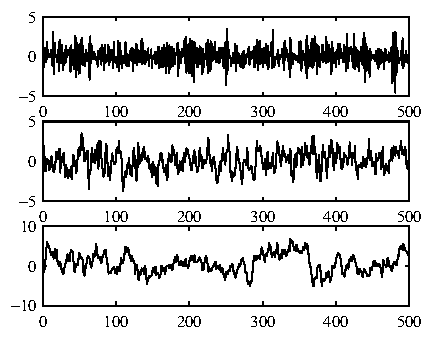
\includegraphics[width=0.6\textwidth]{Figures/chronoar1}\\
  \caption{Trajectoires de longueur $500$ d'un processus AR$(1)$ gaussien.
 Courbe du haut~: $\phi_1=-0.7$.
 Courbe du milieu~: $\phi_1=0.5$.
 Courbe du bas~: $\phi_1=0.9$}
 \label{fig:figar1}
\end{figure}

La fonction d'autocovariance de $(X_{t})$ solution stationnaire
de~(\ref{eq:recurrenceAR1}) est donn\'ee par la
formule~(\ref{eq:gamm_proc_lin}) qui s'\'ecrit\,;
\begin{align}
\label{eq:autocov:AR1}
\gamma_X(h)&= \sigma^2 \sum_{k=0}^\infty \phi_1^k \bar{\phi_1}\;^{k+h}
= \sigma^2 \frac{\bar{\phi_1}\;^{h}}{1 - |\phi_1|^2}\;,\;
\textrm{ si }h\geq 0\;,\\
&=\overline{\gamma(-h)}\;,\;\textrm{ sinon.}
\end{align}

Lorsque $\phi_1$ est un r\'eel strictement positif, le processus $(X_{t})$ est positivement
corr\'el\'e, dans le sens o\`u tous ses coefficients
d'auto-covariance sont positifs. Les exemples de trajectoires
repr\'esent\'ees sur la figure~\ref{fig:figar1} montrent que des valeurs
de $\phi_1$ proches de 1 correspondent \`a des trajectoires
``persistantes''. Inversement, des
valeurs de $\phi_1$ r\'eelles et n\'egatives conduisent \`a des trajectoires o\`u une valeur positive a tendance \`a \^{e}tre
suivie par une valeur n\'egative.
%====== FIGURE
\begin{figure}
\centering
  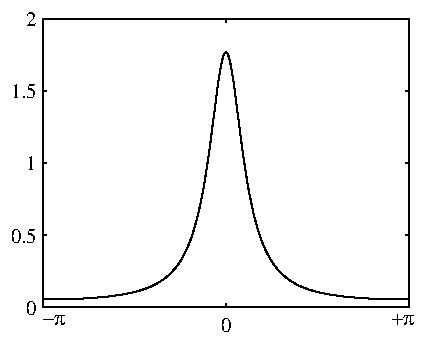
\includegraphics[width=0.6\textwidth]{Figures/dspthAR1}
  \caption{Densit\'e spectrale d'un processus AR(1), d\'efini
  par~(\ref{eq:recurrenceAR1}) pour $\sigma=1$ et $\phi_1=0.7$.}
  \label{fig:dspthAR1}
\end{figure}
la densit\'e spectrale de $(X_t)$ est donn\'ee par
\begin{equation}
\label{eq:dsp:AR1}
 f_X(\lambda)
 = \frac{\sigma^2}{2 \pi} \left| \sum_{k=0}^\infty \phi_1^k \rme^{-\rmi k\lambda} \right|^2
 = \frac{\sigma^2}{2 \pi} \frac{1}{|1 - \phi_1 \rme^{-\rmi \lambda}
   |^2}\; .
\end{equation}
%===============================================
\subsubsection{Cas $|\phi_1| > 1$}
%===============================================
Dans ce cas-l\`a, $\PE{|X_t-\sum_{j=0}^{k}\phi_1^j
Z_{t-j}|^2} = |\phi_1|^{2k+2} \PE{X_{t-k-1}^2}$ diverge
lorsque $k$ tend vers l'infini. Par contre, on peut
r\'e\'ecrire l'\'equation d\'efinissant $X_t$ en fonction de $Z_t$ comme suit
$$
X_t=-\phi_1^{-1} Z_{t+1}+\phi_1^{-1} X_{t+1}.
$$
En it\'erant l'\'equation pr\'ec\'edente, on obtient
\begin{eqnarray*}
X_t&=&-\phi_1^{-1} Z_{t+1}-\phi_1^{-2} Z_{t+2}+\phi_1^{-2} X_{t+2}=\dots\\
&=&-\phi_1^{-1} Z_{t+1}-\phi_1^{-2} Z_{t+2}-\dots-\phi_1^{-k-1}
Z_{t+k+1}+\phi_1^{-k-1} X_{t+k+1}\; .
\end{eqnarray*}
En utilisant exactement les m\^{e}mes arguments que ceux employ\'es
pr\'ec\'edemment, on d\'eduit que la solution stationnaire dans ce cas vaut
\begin{equation}
\label{eq:ar1_sol>1}
X_t=-\sum_{j\geq 1} \phi_1^{-j} Z_{t+j}\; .
\end{equation}
Cette solution est  \textbf{non causale} : elle d\'epend
uniquement du ``futur'' du processus $(Z_t)$.

Remarquons que, comme pr\'ec\'edemment, la solution donn\'ee par \eqref{eq:ar1_sol>1} est obtenu
en choisissant le d\'eveloppement fraction rationnelle $\psi(z)=(1-\phi_1
z^{-1})^{-1}$
\[
  \psi(z)=\frac{1}{1-\phi_1 z^{-1}} = \frac{-(\phi_1 z^{-1})^{-1}}{1-(\phi_1
    z^{-1})^{-1}}=-(\phi_1 z^{-1})^{-1}\sum_{k=0}^{+\infty} (\phi_1 z^{-1})^{-k}
=-\sum_{k\geq 1}\phi_1^{-k} z^{k}\;,
\]
qui converge sur le disque $ \ensemble{ z \in \Cset}{|z| < |\phi_1|}$. Nous remarquons que
nous avons choisi dans les deux cas $|\phi_1| < 1$ et $|\phi_1| > 1$ les d\'eveloppements convergeant
dans des domaines incluant le cercle unit\'e, $\ensemble{ z \in \Cset}{ |z|=1 }$.
Ce choix est justifié pr\'ecis\'ement dans le paragraphe \ref{sec:cas_general}.

%===============================================
\subsubsection{Cas $|\phi_1| = 1$}
%===============================================
Supposons qu'il existe une solution stationnaire dans ce cas alors,
par stationnarit\'e de $X_t$,
$$
\PE{\left|X_t - \sum_{j=0}^{k-1} \phi_1^j Z_{t-j}\right|^2} = |\phi_1|^{2k} \
\PE{|X_{t-k}|^2} = |\phi_1|^{2k}\ \PE{|X_{t}|^2}=\PE{|X_{t}|^2}\;.
$$
Or, le terme de gauche est aussi \'egal \`a
$$
\PE{|X_{t}|^2} + \PE{\left|\sum_{j=0}^{k-1} \phi_1^j Z_{t-j}\right|^2}
- 2 \PE{\bar{X}_{t} \sum_{j=0}^{k-1} \phi_1^j Z_{t-j}}\eqsp.
$$
Ainsi, $\PE{|\sum_{j=0}^{k-1} \phi_1^j Z_{t-j}|^2}
=2 \PE{\bar{X}_{t} \sum_{j=0}^{k-1} \phi_1^j Z_{t-j}}$.
De plus, $\PE{|\sum_{j=0}^{k-1} \phi_1^j Z_{t-j}|^2} = \sum_{j=0}^{k-1}
|\phi_1|^{2j} \sigma^2 = k \sigma^2 $. D'o\`u, en utilisant
l'in\'egalit\'e de Cauchy-Schwarz,
$$
k\sigma^2 \leq 2 \PE{|X_t|^2}^{1/2} \PE{\left|\sum_{j=0}^{k-1}
\phi_1^j Z_{t-j}\right|^2}^{1/2} \leq 2 (\gamma_X(0)+|\mu_X|^2)^{1/2} \
k^{1/2} \sigma \eqsp,
$$
ce qui est impossible pour $k$ grand.
Donc, dans ce cas, \textbf{il n'existe pas de solution stationnaire}.

\subsubsection{Conclusion}

Nous avons donc montr\'e, dans le cas $p=1$, que l'\'equation de  r\'ecurrence
(\ref{eq:recurrenceARp}) n'admettait pas de solution stationnaire
lorsque $|\phi_1|=1$ et qu'elle admettait une solution stationnaire
lorsque $|\phi_1|\neq 1$, donn\'ee par :
$$
X_t=\sum_{j\geq 0}\phi_1^j Z_{t-j}\;, \textrm{ si } |\phi_1|<1\;,
$$
et
$$
X_t=-\sum_{j\geq 1} \phi_1^{-j} Z_{t+j}\;, \textrm{ si } |\phi_1|>1\;.
$$

%
%\begin{definition}[Op\'erateur de retard]
%\label{def:operateur-retard}
%\index{Op\'erateur de retard}
%  Soit $(X_t)_{t\in\Zset}$ d\'efini sur $\espaceproba$ un processus stationnaire au
%  second ordre et soit $\cH^X_\infty$ son enveloppe lin\'eaire.
%D'apr\`es le th\'eor\`eme \ref{theo:prolongement-isometrie}, il existe une unique
%isom\'etrie $B^X$ de  $\cH^X_\infty$ dans $L^2\espaceproba$ telle que
%$B^X(X_t)=X_{t-1}$, pour tout $t\in\Zset$. De plus, $B^X(\cH^X_\infty)=\cH^X_\infty$.
% On appellera $B^X$ l'op\'erateur de retard de $X$ (abr\'eviation de {\em backward} en
%  anglais).
%\end{definition}
%
%On note $(B^X)^k = B^X \circ (B^X)^{k-1}$ pour $k \geq 1$ les compositions successives de
%l'op\'erateur $B^X$.  Pour $k<0$, $(B^X)^k$ est d\'efini comme l'op\'erateur inverse de
%$(B^X)^{-k}$. Cette notation permet d'\'ecrire les \'equations d\'efinissant un processus
%MA et un processus AR d'une fa\c{c}on plus condens\'ee : (\ref{eq:recurrenceMAq})
%se r\'e\'ecrit en : $X_t=\theta(B^Z)Z_t$ et (\ref{eq:recurrenceARp}) se r\'e\'ecrit
%en : $\phi(B^X)X_t=Z_t$ o\`u $\theta(z)=1+\sum_{k=1}^q \theta_k z^k$ et
%$\phi(z)=1-\sum_{k=1}^p \phi_k z^k.$
%%%%%%%%%%%%%%%%%%%%%%%%%%%%%%%%%%%%%%%%%%%%%%%%%%%%%%%%%%%%%%%%%%%%%%%%%%%%%%%%
%%%%%%%%%%%%%%%%%%%%%%%%%%%%%%%%%%%%%%%%%%%%%%%%%%%%%%%%%%%%%%%%%%%%%%%%%%%%%%%%


\subsection{Cas g\'en\'eral}\label{sec:cas_general}
% La notion de processus ARMA g\'en\'eralise les notions de processus MA
% et AR.
Avant d'\'enoncer le th\'eor\`eme \ref{theo:ARMApq} qui donne
une condition n\'ecessaire et suffisante d'existence d'une solution stationnaire
\`a l'\'equation r\'ecurrente \eqref{eq:recurrenceARMApq}
d\'efinissant un processus ARMA($p,q$), nous introduisons un nouvel op\'erateur
qui sera utile dans la preuve du th\'eor\`eme \ref{theo:ARMApq}.

Soit $\cS\espaceproba$ l'ensemble des processus index\'es par $\zset$
stationnaires au second ordre et \`a valeurs complexes. A toute suite de
coefficients complexes $(\alpha_k)$ v\'erifiant :
$\sum_{k\in\Zset}|\alpha_k|<\infty$, on associe un op\'erateur
$\operatorname{F}_\alpha$ qui \`a $X\in\cS\espaceproba$ associe le processus $Y$
d\'efini par :
$$
\operatorname{F}_\alpha:X\mapsto Y=(Y_t)_{t\in\Zset}=\left(\sum_{k\in\Zset}\alpha_k X_{t-k}\right)_{t\in\Zset}\; .
$$
D'apr\`es le th\'eor\`eme \ref{theo:filtragepassl_stat}, $Y$ est aussi dans $\cS\espaceproba$.

Le lemme \ref{lem:composition} montre comment composer deux op\'erateurs
de type $\operatorname{F}_\alpha$.

\begin{lemma}\label{lem:composition}
  Soient $(\alpha_k)$ et $(\beta_k)$ des suites de coefficients complexes
  telles que : $\sum_{k\in\Zset}|\alpha_k|<\infty$ et
  $\sum_{k\in\Zset}|\beta_k|<\infty$.  Si $X\in\cS\espaceproba$ alors
$$
\filtop{\alpha} \circ \filtop{\beta}X = \filtop{\alpha * \beta} X\;, \textrm{
  dans } L^2\espaceproba\;,\;
$$
o\`u $(\alpha*\beta)_k=\sum_{j\in\mathbb{Z}}\alpha_j\beta_{k-j}$ est la convolution discrète des suites $\alpha$ et $\beta$.
\end{lemma}

 \begin{proof}
 Soit $Y=\filtop{\beta}X$. D'apr\`es le th\'eor\`eme \ref{theo:filtragepassl_stat},
puisque $\sum_k|\beta_k|<\infty$, $Y$ est dans $\cS\espaceproba$.
Pour les m\^{e}mes raisons, $\filtop{\alpha}Y$ est lui aussi dans $\cS\espaceproba$.
Soient $Z=\filtop{\alpha}[\filtop{\beta}X]$ et $W=[\filtop{\alpha\beta}]X$, on a alors, pour tout $t\in\Zset$,
$Z_t=\sum_{j\in\Zset}\alpha_j Y_{t-j}$,
o\`u $Y_t=\sum_{k\in\Zset}\beta_k X_{t-k}$ et $W_t=\sum_{k\in\Zset}(\sum_{j\in\mathbb{Z}}\alpha_j\beta_{k-j})X_{t-k}$. Ainsi,
$Z_t=\sum_{j\in\Zset}\alpha_j(\sum_{k\in\Zset}\beta_k X_{t-j-k})$.

D\'efinissons $Z_{t,m,n}$ et $W_{t,m,n}$ par :
$Z_{t,m,n}=\sum_{j=-m}^m\alpha_j(\sum_{k=-n}^n\beta_k X_{t-j-k})$
et $W_{t,m,n}=\sum_{k=-m}^m(\sum_{j=-n}^n\alpha_j\beta_{k-j})X_{t-k}$.
En posant $\ell=j+k$, on en d\'eduit que
\begin{equation}\label{eq:chang_ind}
Z_{t,m,n}=\sum_{\ell=-(m+n)}^{m+n}(\sum_{j=-m}^m\alpha_j\beta_{\ell-j})X_{t-\ell}
=W_{t,m+n,m}\;.
\end{equation}
En notant $\| X \|_2 = \left( \PE{|X|^2} \right)^{1/2}$, nous pouvons
\'ecrire en utilisant l'in\'egalit\'e triangulaire que :
\begin{multline}\label{eq:dec_filtre1}
\|Z_t-W_t\|_2\leq \|Z_t-Z_{t,m,n}\|_2+\|Z_{t,m,n}-W_{t,m+n,m}\|_2
+\|W_{t,m+n,m}-W_t\|_2\;,
\end{multline}
le deuxi\`eme terme du membre de droite de (\ref{eq:dec_filtre1}) \'etant
nul d'apr\`es (\ref{eq:chang_ind}).
D'autre part, avec :
$Z_{t,m}=\sum_{j=-m}^m\alpha_j(\sum_{k\in\Zset}\beta_k X_{t-j-k})
=\sum_{j=-m}^m\alpha_j Y_{t-j}$, on a :
\begin{equation}\label{eq:dec_filtre2}
\|Z_t-Z_{t,m,n}\|_2\leq\|Z_t-Z_{t,m}\|_2+\|Z_{t,m}-Z_{t,m,n}\|_2\;.
\end{equation}
En utilisant l'in\'egalit\'e de Cauchy-Schwarz, le fait que
$Y$ est dans $\cS\espaceproba$ et $\sum_{k\in\Zset}|\alpha_k|<\infty$,  on a
\begin{multline}\label{eq:dec_filtre3}
\|Z_t-Z_{t,m}\|_2^2=\left\|\sum_{|j|>m}\alpha_j Y_{t-j}\right\|_2^2
\leq\PE{\sum_{|j|>m,|j'|>m}|\alpha_j| |\alpha_{j'}| |Y_{t-j}| |Y_{t-j'}|}\\
\leq \PE{Y_0^2}\left(\sum_{|j|>m} |\alpha_j|\right)^2\to 0\;,\; m\to\infty\;.
\end{multline}
D'autre part, en utilisant l'in\'egalit\'e de Cauchy-Schwarz, le fait que
$X$ est dans $\cS\espaceproba$ et l'absolue sommabilit\'e de $(\alpha_k)$
et $(\beta_k)$ :
\begin{align}\label{eq:dec_filtre4}
\|Z_{t,m}-Z_{t,m,n}\|_2^2&=\left\|\sum_{|j|\leq
  m}\alpha_j(\sum_{|k|>n}\beta_k X_{t-j-k})\right\|_2^2\\
&\leq \PE{X_0^2}\left(\sum_{-m\leq j,j'\leq m}|\alpha_j| |\alpha_{j'}|\right)
\left(\sum_{|k|,|k'|>n} |\beta_k||\beta_{k'}|\right)\\
&\leq \PE{X_0^2} \left(\sum_{j\in\Zset}|\alpha_j|\right)^2
\left(\sum_{|k|>n}|\beta_k|\right)^2\to 0\;,\; m,n\to\infty\;.
\end{align}
En utilisant (\ref{eq:dec_filtre2}), (\ref{eq:dec_filtre3}) et
(\ref{eq:dec_filtre4}), on obtient que le premier terme du membre de
droite de (\ref{eq:dec_filtre1}) tend vers 0 lorsque $m$ et $n$
tendent vers l'infini.
On peut montrer en utilisant le m\^{e}me type d'arguments que
$\|W_{t,m+n,m}-W_t\|_2$
tend vers 0 lorsque $m$ et $n$ tendent vers l'infini ce qui conclut la
preuve avec (\ref{eq:dec_filtre1}).

\end{proof}


\begin{theorem}[Existence et unicit\'e des processus ARMA$(p,q)$]
\label{theo:ARMApq} Soit l'\'equation r\'ecurrente~:
\begin{equation}
 \label{eq:recurrenceARMApq}
  X_t - \phi_1 X_{t-1} - \cdots - \phi_p X_{t-p}
  =
  Z_t + \theta_1 Z_{t-1} + \cdots + \theta_q Z_{t-q}\;,
\end{equation} o\`u $Z_t \sim \BB(0,\sigma^2)$ et les
$\phi_j$ et les $\theta_j$ sont des nombres complexes. On note $\phi(z)$ et $\theta(z)$ les transformées en $z$
\begin{align}
\label{eq:tz-phi}
\phi(z)&= 1 - \phi_1 z^{-1} - \dots - \phi_p z^{-p} \\
\label{eq:tz-theta}
\theta(z)&= 1 + \theta_1 z^{-1} + \dots + \theta_q z^{-q}  \eqsp.
\end{align}
On suppose que $\phi(z)$ et $\theta(z)$ n'ont pas de z\'eros communs. Alors l'\'equation
(\ref{eq:recurrenceARMApq}) admet une solution stationnaire au
second ordre si et seulement si le polyn\^ome $\phi(z) \neq 0$ pour
$|z| = 1$. Cette solution est unique et a pour expression~:
\begin{equation}
 \label{eq:solutionARMApq}
 X_t = \sum_{k=-\infty}^{\infty} \psi_k Z_{t-k}\;,
\end{equation}
o\`u les $(\psi_k)$ sont donn\'es par les coefficients du d\'eveloppement
\begin{equation}\label{eq:dev_laurent_statio}
\frac{\theta(z)}{\phi(z)}=\sum_{k\in\Zset}\psi_k z^{-k}\;,
\end{equation}
convergeant dans la couronne
\begin{equation}
\label{eq:RC-psi}
\ensemble{ z\in\cset}{\delta_1<|z|<\delta_2} \eqsp,
\end{equation}
o\`u $\delta_1<1$ et $\delta_2>1$ sont d\'efinis par
\begin{equation}
\label{eq:definition-delta1}
\delta_1=\max\{ z \in \cset, | z | < 1, \phi(z) =0 \}
\end{equation}
et
\begin{equation}
\label{eq:definition-delta2}
\delta_2=\min \{ z \in \cset, |z| > 1, \phi(z) = 0 \} \eqsp,
\end{equation}
\end{theorem}
avec la convention $\max \emptyset = 0$ et $\min \emptyset = \infty$.
\begin{proof}
Nous commen\c{c}ons par \'enoncer et prouver un lemme utile pour la preuve
du th\'eor\`eme \ref{theo:ARMApq}.
%\emnote{il faut se faire une religion ici sur la fa\c{c}on de noter les polynomes, pour le moment on est plut\^ot
%avec des petites lettres grecques, non.. ?}
\begin{lemma}\label{lem:dev_laurent}
  Soient $\theta$ et $\phi$ deux polyn\^omes \`a coefficients complexes tels que
  $\phi(z) \neq 0$ pour $|z|=1$ et $\phi(0)=1$ alors la fraction rationnelle
  $\theta(z)/\phi(z)$ est d\'eveloppable en s\'erie de Laurent, c'est-\`a-dire
$$
\frac{\theta(z)}{\phi(z)}=\sum_{k\in\Zset} c_k z^{-k}\;,
$$
o\`u la s\'erie $\sum_{k \in \zset} c_k z^{-k}$ est uniform\'ement convergente dans la
couronne d\'efinie par
$\left\{ z\in\cset \eqsp, r_1<|z|<r_2 \right\}$, o\`u
\begin{align*}
r_1&=\max\{ |z|~:~ z \in \cset, | z | < 1, \,\phi(z) =0 \}\\
r_2&=\min\{ |z|~:~ z  \in \cset, |z| > 1, \,\phi(z) = 0 \}\; .
\end{align*}
avec la convention $\max(\emptyset)=0$ et $\min(\emptyset)=\infty$.

Le cas $r_1=0$ correspond \`a $\phi(z)\neq0$ dans le disque unité, 
$\ensemble{z \in \cset}{|z|\leq1}$. 
%Dans ce cas on a $c_k=0$ pour tout $k>0$.
%Sinon, pour tout $\eta\in(0,r_1)$, $c_k=O(\eta^{-k})$ quand $k\to +\infty$.

Le cas $r_2=\infty$ correspond \`a $\phi(z)\neq0$ dans la couronne $\ensemble{z \in \cset}{|z| \geq 1}$. Dans ce cas on a $c_k=0$ pour tout $k>\max(-1,\mathrm{deg}(\theta)
- \mathrm{deg}(\phi))$.  
%Sinon, pour tout $\eta\in(0,1/r_2)$, $c_k=O(\eta^{k})$
%quand $k\to\infty$.
\end{lemma}
\begin{proof}\smartqed
  La d\'ecomposition en \'el\'ements simples de la fraction rationnelle
  $\theta(z)/\phi(z)$ s'\'ecrit comme la somme d'un polyn\^ome de degr\'e
  $\mathrm{deg}(\theta) - \mathrm{deg}(\phi)$ (avec la convention que tout
  polyn\^ome de degr\'e strictement n\'egatif est le polyn\^ome nul) et de termes de la forme~:
  $a/(z-z_0)^r$, o\`u $z_0$ est une racine de $\phi$ de multiplicit\'e sup\'erieure
  ou \'egale \`a $r$ et $a$ est une constante.  On \'ecrit :
\begin{align*}
\textrm{si }|z_0|<1,& \;
\frac{1}{(1-z_0 z^{-1})^r}=\frac{z^{-r}}{(1-z_0/z)^r},\;
\textrm{lorsque }|z_0|<|z|\;,\\
\textrm{si }|z_0|>1,& \;
\frac{1}{(z-z_0)^r}=\frac{(-z_0)^{-r}}{(1-z/z_0)^r},\;
\textrm{lorsque }|z|<|z_0|\;.
\end{align*}
%\emnote{ce n'est que le DL de $(1-u)^\alpha$ on n'a pas besoin de trop disserter dessus}
On utilise que :
\begin{multline*}
(1-u)^{-r}=\frac{(-1)^{r-1}}{(r-1)!}\sum_{k\geq r-1}\frac{k!}{(k-r+1)!}
u^{k-r+1}\\
=\frac{(-1)^{r-1}}{(r-1)!}\sum_{k\geq 0}\frac{(k+r-1)!}{k!}
u^{k}\;,\textrm{ lorsque }|u|<1\;,
\end{multline*}
Ainsi,
\begin{align*}
&\textrm{si }|z_0|<1, \;
\frac{1}{(z-z_0)^r}=\frac{z^{-r}}{(1-z_0/z)^r}
=z^{-r}\frac{(-1)^{r-1}}{(r-1)!}\sum_{k\geq 0}\frac{(k+r-1)!}{k!}(z_0/z)^k,\; \\
&\textrm{qui converge si }|z_0|<|z|\;,\\
&\textrm{si }|z_0|>1, \;
\frac{1}{(z-z_0)^r}=\frac{(-z_0)^{-r}}{(1-z/z_0)^r}
=-\frac{z_0^{-r}}{(r-1)!}\sum_{k\geq 0}\frac{(k+r-1)!}{k!}
(z/z_0)^k,\; \\
&\textrm{qui converge si }|z|<|z_0|\;.
\end{align*}
En majorant $(k+r-1)!/k!$ par $k^{r-1}$, on en d\'eduit  que
\begin{align*}
&\textrm{si }|z_0|<1, \;
\frac{1}{(z-z_0)^r}=\sum_{k\leq -r} v_k z^k,\; \textrm{qui converge si }|z|>|z_0|\;,\\
&\textrm{si }|z_0|>1, \;
\frac{1}{(z-z_0)^r}=\sum_{k\geq 0} w_k z^k,\;\textrm{qui converge si }|z|<|z_0|\;,
\end{align*}
o\`u $|v_k|$ et $|w_k|$ sont major\'es par $C \eta^{|k|}$, $C$ \'etant une constante
strictement positive pour tout $\eta$ choisi dans
$(0,r_1)$ ou $(0,1/r_2)$, respectivement.

\end{proof}

\textbf{Retour \`a la preuve du th\'eor\`eme \ref{theo:ARMApq}}\\

Supposons que $\phi(z)\neq 0$ pour $|z|= 1$, alors d'apr\`es
le \Cref{lem:dev_laurent} il existe $r_1<1$ et $r_2>1$ tels que
\begin{equation}\label{eq:psi_arma}
\psi(z)=\frac{\theta(z)}{\phi(z)}=\sum_{k=-\infty}^{\infty} \psi_k z^{-k},\; r_1<|z|<r_2\;,
\end{equation}
o\`u la suite $(\psi_k)_{k\in\Zset}$ v\'erifie $\sum_k |\psi_k|<\infty$.
V\'erifions que le processus $(X_t)$ d\'efini par : $X_t=\sum_{k\in\Zset} \psi_k Z_{t-k}=(\filtop{\psi} Z)_t$, pour tout
$t\in\Zset$ est une solution stationnaire de (\ref{eq:recurrenceARMApq}). D'apr\`es la d\'efinition
\ref{def:proc_lin}, $(X_t)$ est stationnaire. De plus, d'apr\`es le \Cref{lem:composition},
$$
\filtop{\phi} \circ \filtop{\psi} Z =\filtop{\phi*\psi}Z=\filtop{\theta}Z \eqsp,
$$
ce qui montre l'existence d'une solution
stationnaire \`a \eqref{eq:recurrenceARMApq}.

D'autre part, si $X$ est un processus stationnaire au second ordre solution de
(\ref{eq:recurrenceARMApq}) alors $X$ v\'erifie :
\begin{equation}\label{eq:arma_F}
\filtop{\phi} X=\filtop{\theta}Z\;.
\end{equation}
Comme $\phi(z)\neq 0$ pour $|z|= 1$, alors d'apr\`es le
\Cref{lem:dev_laurent} il existe $r_1<1$ et $r_2>1$ tels que :
$$
\xi(z)=\frac{1}{\phi(z)}=\sum_{k\in\Zset} \xi_k z^{k},\; r_1<|z|<r_2\;,
$$
o\`u la suite $(\xi_k)_{k\in\Zset}$ v\'erifie $\sum_k |\xi_k|<\infty$.
On peut donc appliquer l'op\'erateur $\filtop{\xi}$ aux deux membres de l'\'equation
(\ref{eq:arma_F}) d'o\`u l'on d\'eduit en utilisant le lemme \ref{lem:composition}
que $X=\filtop{\xi\theta}Z=\filtop\psi Z$ o\`u $(\psi_k)$ est d\'efinie dans (\ref{eq:psi_arma}).
Donc $X_t=\sum_{k\in\Zset} \psi_k Z_{t-k}=(\filtop{\psi} Z)_t$, pour tout
$t\in\Zset$, ce qui assure l'unicit\'e de la solution.

R\'eciproquement, si $(X_t)$ est un processus stationnaire solution de (\ref{eq:recurrenceARMApq}) de la forme
$X_t=\sum_{k\in\Zset}\eta_k Z_{t-k}$ o\`u $\sum_k |\eta_k|<\infty$, montrons que
$\phi(z)\neq 0$ pour $|z|= 1$. En effet, puisque $X$ est solution de (\ref{eq:arma_F})
alors : $\filtop{\phi} X=\filtop{\phi}[\filtop{\eta} Z]=\filtop{\theta} Z$. D'apr\`es le lemme \ref{lem:composition},
$\filtop{\phi\eta}Z=\filtop{\theta} Z$. Posons
$\zeta_k=\sum_{j\in\Zset}\phi_j \eta_{k-j}$. On a alors, pour tout $t\in\Zset$,
$\sum_{k\in\Zset}\zeta_k Z_{t-k}=\sum_{j=1}^q\theta_j Z_{t-j}.$
En multipliant les deux membres de cette \'equation par $Z_{t-\ell}$
et en prenant l'esp\'erance, on d\'eduit que $\zeta_\ell=\theta_\ell$,
$\ell=0,\dots,q$ et $\zeta_\ell=0$, sinon. Ainsi,
$\theta(z)=\phi(z)\eta(z)$, $|z|=1$. Puisque $\theta$ et $\phi$
n'ont pas de racines communes et que $|\eta(z)|\leq\sum_{k\in\Zset}|\eta_k|<\infty$,
si $|z|=1$, $\phi(z)$ ne s'annule pas sur le cercle unit\'e :
$\{z,\; |z|=1\}$, ce qui conclut la preuve du th\'eor\`eme \ref{theo:ARMApq}.

% Supposons que $\phi(z)\neq 0$ pour $|z|= 1$, alors d'apr\`es le lemme
% \ref{lem:dev_laurent} il existe $r_1<1$ et $r_2>1$ tels que
% $$
% \psi(z)=\frac{\theta(z)}{\phi(z)}=\sum_{k=-\infty}^{\infty} \psi_k z^{k},\; r_1<|z|<r_2\;,
% $$
% o\`u la suite $(\psi_k)_{k\in\Zset}$ v\'erifie $\sum_k |\psi_k|<\infty$.
% V\'erifions que $X_t=\sum_{k\in\Zset} \psi_k Z_{t-k}=\psi(B^Z)Z_t$ pour tout
% $t\in\Zset$ est une solution stationnaire de (\ref{eq:recurrenceARMApq}). D'apr\`es la d\'efinition
% \ref{def:proc_lin}, $(X_t)$ est stationnaire. De plus, par d\'efinition, $\cH^X_\infty\subset\cH^Z_\infty$ et
% d'apr\`es le lemme \ref{lem:composition},
% $\phi(B^Z)X_t=\phi(B^Z)\psi(B^Z)Z_t=(\phi\psi)(B^Z)Z_t=\theta(B^Z)Z_t.$
% Montrons que cette solution est unique. Pour cela, notons En effet, soit $(Y_t)$ un autre processus stationnaire
% solution de (\ref{eq:recurrenceARMApq}) alors :
% $(X_t-Y_t)-\sum_{k=1}^p\phi_k(X_{t-k}-Y_{t-k})=0$


% R\'eciproquement, si $X_t$ est une solution stationnaire de (\ref{eq:recurrenceARMApq}) de la forme
% $X_t=\sum_{k\in\Zset}\eta_k Z_{t-k}$ o\`u $\sum_k |\eta_k|<\infty$
% alors : $\phi(B^X)X_t=\phi(B^Z)\eta(B^Z)Z_t=\theta(B^Z)Z_t$. D'apr\`es le lemme \ref{lem:composition},
% $(\phi\eta)(B^Z)Z_t=\theta(B^Z)Z_t$. Posons
% $\zeta(z)=\phi(z)\eta(z)=\sum_{k\in\Zset}\zeta_k z^k$, lorsque $|z|=1$. On a alors,
% $\sum_{k\in\Zset}\zeta_k Z_{t-k}=\sum_{j=1}^q\theta_j Z_{t-j}.$
% En multipliant les deux membres de cette \'equation par $Z_{t-\ell}$
% et en prenant l'esp\'erance, on d\'eduit que $\zeta_\ell=\theta_\ell$,
% $\ell=0,\dots,q$ et $\zeta_\ell=0$, sinon. Ainsi,
% $\theta(z)=\phi(z)\eta(z)$, $|z|=1$. Puisque $\theta$ et $\phi$
% n'ont pas de racines communes et que $|\eta(z)|\leq\sum_{k\in\Zset}|\eta_k|<\infty$,
% si $|z|=1$, $\phi(z)$ ne s'annule pas sur le cercle unit\'e :
% $\{z,\; |z|=1\}.$

\end{proof}
Dans le cas o\`u $\phi(z)$ et $\theta(z)$ ont des z\'eros communs,
deux configurations sont possibles~:
\begin{enumerate}[label=(\alph*)]
\item Les z\'eros communs ne sont pas sur le cercle unit\'e. Dans ce
cas on se
  ram\`ene au cas sans z\'ero commun en annulant les facteurs communs.
\item Certains des z\'eros communs se trouvent sur le cercle unit\'e.
  L'\'equation~(\ref{eq:recurrenceARMApq}) admet une infinit\'e de solutions
  stationnaires au second ordre.
\end{enumerate}
Du point de vue de la mod\'elisation, la pr\'esence de z\'eros communs
ne pr\'esente aucun int\'er\^{e}t puisqu'elle est sans influence sur
la densit\'e spectrale de puissance. Elle conduit de plus \`a une
ambigu\"{i}t\'e sur l'ordre r\'eel des parties AR et MA.
%=========================================================
\subsubsection{ARMA$(p,q)$ causal}
%  Comme dans le cas d'un processus AR($p$), on peut
% distinguer trois cas, suivant que les z\'eros de $\phi(z)$ sont \`a
% l'ext\'erieur, \`a l'int\'erieur ou de part et d'autre du cercle unit\'e.
% Dans le cas o\`u les z\'eros de $\phi(z)$ sont \`a l'ext\'erieur du
% cercle unit\'e, la suite $\xi_k$ est causale ($\xi_k=0$ pour $k<0$)
% et donc $\psi_k=\xi_k+\sum_{j=1}^q \theta_j\xi_{k-j}$ est aussi
% causale. Par cons\'equent le processus $X_t$ s'exprime causalement
% en fonction de $Z_t$.
Le th\'eor\`eme \ref{theo:ARMApq_causal} donne une condition n\'ecessaire
et suffisante d'existence d'une solution causale \`a l'\'equation
(\ref{eq:recurrenceARMApq}).

\begin{definition}[Repr\'esentation ARMA causale]
  Sous les hypoth\`eses du th\'eor\`eme~\ref{theo:ARMApq}, on dira que
  l'\'equation~(\ref{eq:recurrenceARMApq}) fournit une repr\'esentation causale de
  la solution stationnaire au second ordre $(X_t)$ si $(X_t)_{t\in\zset}$ est
  un processus lin\'eaire causal par rapport \`a $(Z_t)_{t\in\zset}$.
\end{definition}

\begin{theorem}[ARMA$(p,q)$ causal]
\label{theo:ARMApq_causal}
Soit l'\'equation r\'ecurrente~:
\begin{equation}
 \label{eq:recurrenceARMApqcausal}
  X_t - \phi_1 X_{t-1} - \cdots - \phi_p X_{t-p}
  =
  Z_t + \theta_1 Z_{t-1} + \cdots + \theta_q Z_{t-q}
\end{equation} o\`u $Z_t \sim \BB(0,\sigma^2)$ et
$\{ \phi_j \}_{j = 1}^p$ et $\{ \theta_j \}_{j=1}^q$ sont des nombres complexes. On pose
$\phi(z)= 1 - \phi_1 z^{-1} - \dots - \phi_p z^{-p}$ et $\theta(z)= 1 +
\theta_1 z^{-1} + \dots + \theta_p z^{-p}$. On suppose que $\phi(z)$ et
$\theta(z)$ n'ont pas de z\'eros communs. Alors l'\'equation
(\ref{eq:recurrenceARMApqcausal})
fournit une repr\'esentation causale de la solution stationnaire au second ordre
si et seulement si le polyn\^ome $\phi(z)
\neq 0$ pour $|z| \geq 1$. Cette solution a pour
expression~:
\begin{equation}
 \label{eq:solutionARMApq_causal}
  X_t = \sum_{k\geq 0} \psi_k Z_{t-k}
\end{equation}
o\`u la suite $(\psi_k)$ est donn\'ee par les coefficients du d\'eveloppement
$$
\frac{\theta(z)}{\phi(z)}=\sum_{k=0}^{\infty} \psi_k z^{-k}
$$
qui converge dans la couronne $\{z\in\cset\;,\;|z|\geq 1\}.$
\end{theorem}
\begin{proof}\smartqed
Le th\'eor\`eme~\ref{theo:ARMApq} montre l'existence et l'unicit\'e
de la solution de l'\'equation~(\ref{eq:recurrenceARMApqcausal}) et v\'erifie
\begin{equation*}
  X_t = \sum_{k\in\zset} \psi_k Z_{t-k}
\end{equation*}
o\`u la suite $(\psi_k)$ est caract\'eris\'ee par l'\'equation
$$
\frac{\theta(z)}{\phi(z)}=\sum_{k=0}^{\infty} \psi_k z^{-k},\quad z\in\cset,\,|z|=1\;.
$$
Si maintenant $\phi(z)\neq 0$ pour $|z|\leq 1$, alors, d'apr\`es le
 lemme \ref{lem:dev_laurent}, comme $r_1=0$, on a $\psi_k=0$ pour $k<0$
 et~(\ref{eq:solutionARMApq_causal}) suit.


R\'eciproquement, si $X$ est une solution stationnaire de
(\ref{eq:recurrenceARMApqcausal}) de la forme $X_t=\sum_{k\geq 0}\eta_k
Z_{t-k}$ o\`u $\sum_k |\eta_k|<\infty$, montrons que $\phi(z)\neq 0$ pour
$|z|\leq 1$. En effet, puisque $X$ est solution
de~(\ref{eq:recurrenceARMApqcausal}), alors : $\filtop{\phi}
X=\filtop{\phi}[\filtop{\eta} Z]=\filtop{\theta} Z$. D'apr\`es le lemme
\ref{lem:composition}, $\filtop{\phi\eta}Z=\filtop{\theta} Z$. Posons, pour
tout $k\in\mathbb{N}$, $\zeta_k=\sum_{j\geq 0}\phi_j \eta_{k-j}$, o\`u par
convention, $\eta_\ell=0$, si $\ell<0$.  On a alors, pour tout $t\in\Zset$,
$\sum_{k\geq 0}\zeta_k Z_{t-k}=\sum_{j=0}^q\theta_j Z_{t-j},$ avec la
convention $\theta_0=1$.  En multipliant les deux membres de cette \'equation par
$Z_{t-\ell}$ et en prenant l'esp\'erance, on d\'eduit que $\zeta_\ell=\theta_\ell$,
$\ell=0,\dots,q$ et $\zeta_\ell=0$, sinon. Ainsi, $\theta(z)=\phi(z)\eta(z)$,
$|z|\leq 1$. Puisque $\theta$ et $\phi$ n'ont pas de racines communes et que
$|\eta(z)|\leq\sum_{k\geq 0}|\eta_k|<\infty$, si $|z|\leq 1$, $\phi(z)$ ne
s'annule pas sur le disque unit\'e : $\{z,\; |z|\leq 1\}$, ce qui conclut la
preuve du th\'eor\`eme~\ref{theo:ARMApq_causal}.

\end{proof}
%==========================================


\begin{definition}[Repr\'esentation ARMA inversible]
  Sous les hypoth\`eses du th\'eor\`eme~\ref{theo:ARMApq}, on dira que
  l'\'equation~(\ref{eq:recurrenceARMApq}) fournit une repr\'esentation inversible
  de la solution stationnaire au second ordre $(X_t)$ si $(X_t)_{t\in\zset}$
  est un processus lin\'eaire inversible par rapport \`a $(Z_t)_{t\in\zset}$.
\end{definition}

\begin{theorem}[ARMA$(p,q)$ inversible]
 \label{theo:ARMAinversible}
Soit l'\'equation r\'ecurrente~:
\begin{equation}
 \label{eq:recurrenceARMApqinversible}
  X_t - \phi_1 X_{t-1} - \cdots - \phi_p X_{t-p}
  =
  Z_t + \theta_1 Z_{t-1} + \cdots + \theta_q Z_{t-q}
\end{equation} o\`u $Z_t \sim \BB(0,\sigma^2)$ et les
$\phi_j$ et les $\theta_j$ sont des nombres complexes. On pose
$\phi(z)= 1 - \phi_1 z - \dots - \phi_p z^p$ et $\theta(z)= 1 +
\theta_1 z + \dots + \theta_p z^p$. On suppose que $\phi(z)$ et
$\theta(z)$ n'ont pas de z\'eros communs. Alors l'\'equation
(\ref{eq:recurrenceARMApqinversible}) fournit une repr\'esentation inversible
de la solution stationnaire au second ordre si et seulement si le polyn\^ome $\theta(z)
\neq 0$ pour $|z| \leq 1$. Cette solution est unique et a pour
expression~:
\begin{equation}
 \label{eq:solutionARMApq_inversible}
  Z_t = \sum_{k\geq 0} \pi_k X_{t-k}
\end{equation}
o\`u la suite $(\pi_k)$ est donn\'ee par les coefficients du d\'eveloppement
$$
\frac{\phi(z)}{\theta(z)}=\sum_{k=0}^{\infty} \pi_k z^{-k}
$$
qui converge dans $\{z\in\cset\;,\;|z|\leq 1\}.$
% Soit $X_t$ un processus ARMA$(p,q)$. On suppose que $\phi(z)$ et
% $\theta(z)$ n'ont pas de z\'eros communs. Alors il existe une suite
% $\{\pi_k\}$ causale absolument sommable telle que~:
% \begin{equation}
%  \label{eq:analyseARMApq}
%  Z_t=\sum_{k=0}^{\infty} \pi_k X_{t-k}
% \end{equation}
% si et seulement si $\theta(z)\neq 0$ pour $z\leq 1$. On dit alors
% que le mod\`ele ARMA$(p,q)$ est inversible. La suite $\pi_k$ est
% la suite des coefficients du d\'eveloppement en s\'erie de
% $\phi(z)/\theta(z)$ dans le disque $\{z: |z|\leq 1\}$.
\end{theorem}
La preuve de ce th\'eor\`eme est tout \`a fait analogue \`a celle du
th\'eor\`eme~\ref{theo:ARMApq_causal} et n'est donc pas d\'etaill\'ee ici.
% Remarquons que la notion d'inversibilit\'e, comme celle de causalit\'e, est bien relative au
% mod\`ele ARMA$(p,q)$ lui-m\^{e}me et pas uniquement au processus
% $X_t$.
%\begin{exercice}
%  Soit $X_t$ un processus stationnaire au second ordre solution de l'\'equation
%  de r\'ecurrence~(\ref{eq:recurrenceARMApqcausal}) o\`u le mod\`ele ARMA$(p,q)$
%  correspondant est suppos\'e sans z\'ero commun mais pas n\'ecessairement
%  inversible. Montrer qu'il existe un bruit blanc $\tilde{Z}_t$ tel que $X_t$
%  soit solution de
%  \[
%    \phi(B) X_t = \tilde{\theta}(B) \tilde{Z}_t
%  \]
%  o\`u le mod\`ele ARMA$(p,q)$ d\'efini par $\phi_1, \dots \phi_p$ et
%  $\tilde{\theta}_1, \dots \tilde{\theta}_q$ est inversible
%  (indication\,: consid\'erer des facteurs passe-tout).
%\end{exercice}

Un mod\`ele ARMA$(p,q)$ est causal et inversible lorsque
les racines des polyn\^omes $\phi(z)$ et $\theta(z)$ sont toutes
situ\'ees \`a l'ext\'erieur du disque unit\'e. Dans ce cas, $X_t$ et $Z_t$
se d\'eduisent mutuellement l'un de l'autre par des op\'erations de
filtrage causal.
%, la r\'eponse impulsionnelle de chacun de ces
%filtres \'etant {\em \`a phase minimale} (c'est \`a dire inversible
%causalement).

\subsubsection{Calcul des covariances d'un processus ARMA$(p,q)$ causal}
Une premi\`ere m\'ethode consiste \`a utiliser l'expression
(\ref{eq:gamm_proc_lin}) % qui s'\'ecrit, compte tenu du fait que
% $\{Z_t\}$ est un bruit blanc,
% $$
%  \gamma(h)=
%    \sigma^2 \sum_{k=0}^\infty\psi_k \psi_{k+|h|}
%    $$
   o\`u la suite $(\psi_k)$ se d\'etermine de fa\c{c}on r\'ecurrente \`a partir de
   l'\'egalit\'e $\psi(z)\theta(z)=\phi(z)$ par identification du terme en $z^k$.
   Pour les premiers termes on trouve~:
\begin{eqnarray*}
 &&\psi_0=1\\
 &&\psi_1=\theta_1+\psi_0\phi_1\\
 &&\psi_2=\theta_2+\psi_0\phi_2+\psi_1\phi_1\\
 &&\cdots
\end{eqnarray*}
La seconde m\'ethode utilise une formule de r\'ecurrence, v\'erifi\'ee par
la fonction d'autocovariance d'un processus ARMA$(p,q)$, qui
s'obtient en multipliant les deux membres de
(\ref{eq:recurrenceARMApq}) par $\bar{X}_{t-k}$ et en prenant
l'esp\'erance. On obtient~:
\begin{align}
 \label{eq:recurrencegamma1}
  &\gamma(k)-\phi_1\gamma(k-1)-\cdots-\phi_p\gamma(k-p)
  =
  \sigma^2\sum_{k\leq j\leq q}\theta_j\bar{\psi}_{j-k}\;,\;
0\leq k < \max(p,q+1)
  \\
 \label{eq:recurrencegamma2}
  &\gamma(k)-\phi_1\gamma(k-1)-\cdots-\phi_p\gamma(k-p)
  =
  0\;,\; k \geq \max(p,q+1)
\end{align}
o\`u nous avons utilis\'e la causalit\'e du processus pour \'ecrire
que $\PE{Z_t \bar{X}_{t-k}}=0$ pour tout $k\geq 1$. Le calcul de la
suite $\{\psi_k\}$ pour $k=1,\dots, p$ se fait comme pr\'ec\'edemment.
En reportant ces valeurs dans~(\ref{eq:recurrencegamma1}) pour
$0\leq k \leq p$, on obtient $(p+1)$ \'equations lin\'eaires aux
$(p+1)$ inconnues $(\gamma(0),\dots,\gamma(p))$ que l'on peut
r\'esoudre. Pour d\'eterminer les valeurs suivantes on utilise
l'expression (\ref{eq:recurrencegamma2}).
\subsubsection{Densit\'e spectrale d'un processus ARMA$(p,q)$}
\begin{theorem}[Densit\'e spectrale d'un processus ARMA$(p,q)$]
Soit $(X_t)$ un processus ARMA$(p,q)$ (pas n\'ecessairement causal ou
inversible) \textit{i.e.} la solution stationnaire de l'\'equation
(\ref{eq:recurrenceARMApq}) o\`u les polyn\^omes $\theta(z)$ et $\phi(z)$ sont des
polyn\^omes de degr\'e $q$ et $p$ n'ayant pas de z\'eros communs. Alors
$(X_t)$ poss\`ede une densit\'e spectrale qui a pour expression~:
\begin{equation}
 \label{eq:dspARMApq}
 f(\lambda)=\frac{\sigma^2}{2\pi}
    \frac{\left| 1+\sum_{k=1}^q \theta_k \rme^{-\rmi k \lambda}\right|^2}
         {\left| 1-\sum_{k=1}^p \phi_k \rme^{-\rmi k \lambda}\right|^2}\;,\; -\pi\leq\lambda\leq\pi\;.
\end{equation}
\end{theorem}

\begin{remark}
D'apr\`es le th\'eor\`eme \ref{theo:ARMApq}, l'expression de $f$ est bien
d\'efinie puisque $\phi$ ne s'annule pas sur le cercle unit\'e.
\end{remark}





%%% Local Variables:
%%% mode: latex
%%% ispell-local-dictionary: "francais"
%%% TeX-master: "../monographie-serietemporelle"
%%% End:

\chapter{Pr\'ediction des signaux al\'eatoires}
\label{chap:Prediction}
% \section{th\'eor\`eme de Projection}
%     \subsection{Espace de Hilbert}
%     \subsection{Bases orthonormales}
%     \subsection{th\'eor\`eme de projection}
% \section{Algorithmes de Levinson-Durbin}
%================================================
%================================================
\section{Pr\'ediction lin\'eaire de processus stationnaires}
%================================================
% %================================================
% \subsection{Estimation lin\'eaire en moyenne quadratique}
% %================================================
% Soient $X$ et $\{Y_1,\cdots,Y_p\}$ des variables al\'eatoires
% r\'eelles de $L^2(\Omega,\cF,\PP)$. On cherche \`a
% d\'eterminer la meilleure approximation de $X$ par une combinaison
% lin\'eaire des variables $Y_k$. Nous supposons ici que nous
% connaissons les quantit\'es $\mu=\PE{X}$, $\nu_k=\PE{Y_k}$ ainsi
% que les coefficients de covariance $\cov(X,Y_k)$ et
% $\cov(Y_k,Y_{\ell})$, pour tout $1\leq k,\ell\leq p$. En pratique,
% nous verrons au chapitre~\ref{chap:estim-lineaire}
% comment il est possible, sous certaines hypoth\`eses, de construire des
% estimateurs consistants et asymptotiquement normaux de ces quantit\'es \`a partir d'une suite
% d'observations.

% On consid\`ere l'espace ferm\'e de dimension
% finie ${\cal Y} = \lspan{1, Y_1,\cdots,Y_p}$ et on cherche
% l'\'el\'ement $Y\in \cY$ qui minimise la norme de le risque quadratique
% $\| X - Y\|^2$. Il d\'ecoule imm\'ediatement du th\'eor\`eme de
% projection que le pr\'edicteur lin\'eaire optimal est la projection
% orthogonale $\proj{X}{\cY}$ de $X$ sur ${\cal Y}$ qui v\'erifie
% $(X-\proj{X}{\cY})\perp {\cal Y}$. On en d\'eduit que\,:
% \begin{gather}
% \label{eq:reglin1}
% \begin{cases}
%  \pscal{X - \proj{X}{\cY}}{1} = 0  &\\
%  \pscal{X - \proj{X}{\cY}}{Y_k} = 0 &\text{pour $k \in \{1, \cdots, p \}$}
% \end{cases}  \eqsp.
% \end{gather}
% Ce sont ces $(p+1)$ \'equations qui vont nous donner la solution
% cherch\'ee. En effet la condition $\proj{X}{\cY} \in \cY$ implique (comme $\cY$ est de
% dimension finie) que $\proj{X}{\cY}=a_0 + \sum_{k=1}^p a_k (Y_k - \nu_k)$.
% Il suffit donc de calculer $a_0,a_1,\dots,a_p$. Partant de la premi\`ere expression de
% \eqref{eq:reglin1}, on obtient\,:
% \begin{equation}
%  \label{eq:ortho0}
%  \pscal{X - a_0 - \sum_{k=1}^p a_k (Y_k - \nu_k)}{1} = \pscal{X}{1} - a_0 = 0 \eqsp,
% \end{equation}
% qui donne $a_0=\mu$. En posant $a_0=\mu$ dans la seconde
% expression de \eqref{eq:reglin1}, on a obtient alors
% $k\in\{1,\dots,p\}$\,:
% \begin{multline}
%  \label{eq:ortho1p}
%  \pscal{X - \mu - \sum_{j=1}^p a_j (Y_j - \nu_j)}{Y_k - \nu_k}
%  \\= \pscal{X - \mu}{Y_k-\nu_k} - \sum_{j=1}^p a_j \pscal{Y_j - \nu_j}{Y_k - \nu_k} = 0 \eqsp,
% \end{multline}
% qui montrent que $\{a_1, \cdots, a_p\}$ sont solution d'un
% syst\`eme de $p$ \'equations lin\'eaires \`a $p$ inconnues.

% Ce syst\`eme d'\'equations peut se mettre sous forme plus compacte en
% utilisant la matrice $\Gamma = [\cov(Y_k,Y_{\ell})]_{1 \leq k,\ell
% \leq p}$ des coefficients de covariance de $(Y_1, \cdots, Y_p)$ et
% le vecteur $\bfgamma= [\cov (X,Y_1), \cdots, \cov(X,Y_p)]^T$ des
% coefficients de covariance entre $X$ et les composantes $Y_k$.
% Avec ces notations, le vecteur $\bfalpha = [a_1, \cdots, a_p]^T$
% est solution de l'\'equation\,:
% \begin{equation}
% \label{eq:Eqsnormales}
% \Gamma \bfalpha = \bfgamma
% \end{equation}
% Ce syst\`eme lin\'eaire admet une unique solution si la matrice
% $\Gamma$ est inversible. Notons enfin qu'en vertu de l'identit\'e de
% Pythagore, nous avons\,:
% \[
% \| X \|^2 = \| \proj{X}{\cY} \|^2 + \| X - \proj{X}{\cY} \|^2
% \]
% et donc la norme minimale de l'erreur de pr\'ediction a pour
% expression\,:
% \[
% \| X - \proj{X}{\cY} \|^2 = \| X \|^2 - \| \proj{X}{\cY}\|^2 \eqsp.
% \]
% Nous allons \`a pr\'esent appliquer ce r\'esultat \`a la pr\'ediction
% d'un processus stationnaire au second-ordre \`a partir de son
% pass\'e imm\'ediat en prenant $X=X_t$ et $Y_k=X_{t-k}$ avec
% $k=\{1,\dots,p\}$.
%==============================================================
%==============================================================
%\subsection{Pr\'ediction lin\'eaire de processus stationnaires}
%==============================================================
Soit $(X_t)_{t\in\Zset}$ un processus stationnaire au
second ordre \`a valeurs r\'eelles, \textbf{d'esp\'erance nulle} et de fonction
d'autocovariance $\gamma(h)= \cov(X_h,X_0)$. On cherche \`a
\emph{pr\'edire} la valeur du processus \`a la date $t$ \`a partir
d'une combinaison lin\'eaire des $p$ derniers \'echantillons du pass\'e
$X_{t-1}, \dots, X_{t-p}$. La meilleure combinaison lin\'eaire
(\textit{i.e.} le pr\'edicteur lin\'eaire optimal)
est la projection orthogonale de $X_t$ sur
$\cH_{t-1,p}$  not\'ee $\proj{X_t}{\cH_{t-1,p}}$, o\`u $\cH_{t-1,p}$ est
d\'efini par :
\begin{equation}
\label{eq:cht}
\cH_{t-1,p} = \lspan{X_{t-1}, X_{t-2}, \cdots, X_{t-p}}\;.
\end{equation}
Les indices dans la notation $\cH_{t-1,p}$ doivent �tre compris ainsi
: $\cH_{t-1,p}$ est le sous-espace vectoriel engendr\'e par les
$p$ observations pr\'ec\'edant $X_{t-1}$ \`a savoir
$X_{t-1}, \dots, X_{t-p}$.
D'apr\`es le th\'eor\`eme \ref{theo:projection},
\begin{equation}\label{eq:def_phi_kp}
\proj{X_t}{\cH_{t-1,p}}=\sum_{k=1}^p \phi_{k,p} X_{t-k}\;,
\end{equation}
o\`u les coefficients $(\phi_{k,p})_{1\leq k\leq p}$ satisfont
\begin{equation}\label{eq:scal_1}
\left\langle X_t-\sum_{k=1}^p \phi_{k,p} X_{t-k},X_{t-j}\right\rangle=0\;,\;
j=1,\dots,p\;,
\end{equation}
la notation $\left\langle \cdot,\cdot\right\rangle$ correspondant au
produit scalaire dans $\ltwo\espaceproba$ d\'efini pour $X$ et $Y$
dans $\ltwo\espaceproba$ par  $\left\langle X,Y\right\rangle=\PE{XY}$.
L'\'equation (\ref{eq:scal_1}) se r\'e\'ecrit encore sous la forme
\begin{equation}\label{eq:scal_2}
\left\langle X_t,X_{t-j}\right\rangle=\sum_{k=1}^p \phi_{k,p}
\left\langle  X_{t-k},X_{t-j}\right\rangle\;,\;
j=1,\dots,p\;,
\end{equation}
soit encore
\begin{equation}\label{eq:scal_3}
\sum_{k=1}^p \phi_{k,p}\gamma(k-j)=\gamma(j)\;,\;
j=1,\dots,p\;.
\end{equation}
En posant $\Gamma_p$ la matrice de covariance
du vecteur $(X_{t-1},\dots, X_{t-p})$ d\'efinie par
\begin{equation*}
\Gamma_p =
 \left[
 \begin{matrix}
  \gamma(0)  & \gamma(1)  &  \cdots    &            & \gamma(p-1) \\
  \gamma(1)  & \gamma(0)  &  \gamma(1) &            & \vdots \\
  \vdots     &\ddots      &  \ddots    &  \ddots    &     \\
  \vdots     &            &            &            &\gamma(1)  \\
  \gamma(p-1)& \gamma(p-2)&  \cdots    & \gamma(1)  & \gamma(0)
 \end{matrix}
 \right]\;,
\end{equation*}
on peut r\'e\'ecrire (\ref{eq:scal_3}) comme suit :
\begin{equation}\label{eq:YW1}
 \Gamma_p \bfphi_p = \bfgamma_p\;,
\end{equation}
o\`u $\bfphi_p=(\phi_{1,p},\dots,\phi_{p,p})^T$ et
$\bfgamma_p=(\gamma(1), \gamma(2), \cdots, \gamma(p))^T$.

\begin{definition}
\index{Innovation!partielle}
Nous appellerons dans la suite
\emph{erreur de pr\'ediction directe} d'ordre $p$ ou
\emph{innovation partielle} d'ordre $p$ le processus\,:
\begin{equation}
\label{eq:deferreurforward}
 \epsilon_{t,p}^+
 = X_t - \proj{X_t}{\cH_{t-1,p}}
 = X_t - \sum_{k=1}^{p} \phi_{k,p} X_{t-k}\;.
\end{equation}
La variance de l'erreur de pr\'ediction directe d'ordre $p$ est not\'ee
$\sigma_p^2$ et d\'efinie par
\begin{equation}\label{eq:var_pred_dir}
\sigma_p^2=\|X_t - \proj{X_t}{\cH_{t-1,p}}\|^2=\PE{|X_t -
  \proj{X_t}{\cH_{t-1,p}}|^2}\;.
\end{equation}
\end{definition}
D'apr\`es (\ref{eq:def_phi_kp}) et la proposition \ref{prop:projecteur},
la variance de l'erreur de pr\'ediction directe d'ordre $p$ a pour expression :
\begin{equation}
 \label{eq:YW2}
 \sigma_p^2 = \pscal{X_t}{X_t - \proj{X_t}{\cH_{t-1,p}}}
            =\gamma(0)- \sum_{k=1}^p \phi_{k,p}\gamma(k)
            =\gamma(0)-\bfphi_p^T\bfgamma_p\;.
\end{equation}
Les \'equations \eqref{eq:YW1} et \eqref{eq:YW2} sont appel\'ees les
\emph{\'equations de Yule-Walker}.
% Notons la propri\'et\'e importante
% suivante~: pour $p$ fix\'e, la suite des coefficients
% $\{\phi_{k,p}\}_{1\leq k \leq p}$ du pr\'edicteur lin\'eaire optimal
% et la variance de l'erreur minimale de pr\'ediction {\em ne
% d\'ependent pas de $t$}.

Notons que (\ref{eq:YW1}) a une unique solution si et seulement si
la matrice $\Gamma_p$ est inversible auquel cas la solution vaut :
\begin{equation}\label{eq:sol_unique}
\bfphi_p=\Gamma_p^{-1} \bfgamma_p\; .
\end{equation}
La proposition \ref{prop:Gammanrangplein} fournit les conditions suffisantes assurant
que $\Gamma_p$ est inversible pour tout $p$. Une autre preuve de la proposition \ref{prop:Gammanrangplein}
r\'esultat est propos\'ee dans le probl\`eme \ref{prob1:prediction}. On a ainsi des conditions
sous lesquelles on peut calculer le pr\'edicteur de $X_t$ \`a partir de
$X_{t-1},\dots,X_{t-p}$.



% Ce probl\`eme est bien entendu
% un cas particulier du probl\`eme pr\'ec\'edent o\`u nous avons $X=
% X_t$ et $Y_k = X_{t-k}$, pour $k \in \{1, \dots, p \}$ et
% o\`u\,:
% \begin{equation}
% \label{eq:cht}
%   \cH_{t-1,p} = \lspan{1, X_{t-1}, X_{t-2}, \cdots, X_{t-p}}
% \end{equation}
% Formons la matrice de covariance $\Gamma_p$ du vecteur $[X_{t-1},
% \cdots, X_{t-p}]$:
% \begin{equation}
% \Gamma_p =
%  \left[
%  \begin{matrix}
%   \gamma(0)  & \gamma(1)  &  \cdots    &            & \gamma(p-1) \\
%   \gamma(1)  & \gamma(0)  &  \gamma(1) &            & \vdots \\
%   \vdots     &\ddots      &  \ddots    &  \ddots    &     \\
%   \vdots     &            &            &            &\gamma(1)  \\
%   \gamma(p-1)& \gamma(p-2)&  \cdots    & \gamma(1)  & \gamma(0)
%  \end{matrix}
%  \right]
% \end{equation}
% Cette matrice est dite de Toeplitz, ses \'el\'ements \'etant \'egaux
% le long de ses diagonales. Notons $\bfgamma_p$ le vecteur
% $[\gamma(1), \gamma(2), \cdots, \gamma(p)]^T$ le vecteur des
% coefficients de corr\'elation. D'apr\`es l'\'equation
% \eqref{eq:Eqsnormales}, les coefficients $\{\phi_{k,p}\}_{1\leq
% k\leq p}$ du pr\'edicteur lin\'eaire optimal d\'efini par\,:
% \begin{equation}
%  \label{eq:formegenedeXtsurH}
%  \proj{X_t}{\cH_{t-1,p}} - \mu=\sum_{k=1}^p \phi_{k,p} (X_{t-k}-\mu)
% \end{equation}
% sont solutions du syst\`eme d'\'equations\,:
% \begin{equation}
%  \label{eq:YW1}
%  \Gamma_p \bfphi_p = \bfgamma_p \hspace{1cm}
% \end{equation}
% D'autre part l'erreur de pr\'ediction minimale a pour expression\,:
% \begin{eqnarray}
%  \label{eq:YW2}
%  &\sigma_p^2 &= \| X_t - \proj{X_t}{\cH_{t-1,p}}\|^2
%             = \pscal{X_t-\mu}{X_t - \proj{X_t}{\cH_{t-1,p}}} \nonumber \\
%             &&=\gamma(0)- \sum_{k=1}^p \phi_{k,p}\gamma(k)
%             =\gamma(0)-\bfphi_p^T\bfgamma_p
% \end{eqnarray}
% Les \'equations \eqref{eq:YW1} et \eqref{eq:YW2} sont appel\'ees
% \emph{\'equations de Yule-Walker}. Notons la propri\'et\'e importante
% suivante~: pour $p$ fix\'e, la suite des coefficients
% $\{\phi_{k,p}\}_{1\leq k \leq p}$ du pr\'edicteur lin\'eaire optimal
% et la variance de l'erreur minimale de pr\'ediction {\em ne
% d\'ependent pas de $t$}.

% Les \'equations \eqref{eq:YW1} et
% \eqref{eq:YW2} peuvent encore �tre r\'e\'ecrites \`a partir des
% coefficients de corr\'elation $\rho(h)=\gamma(h)/\gamma(0)$. Il
% vient\,:
% \begin{equation}
%  \label{eq:YWcorrelation}
%  \left[
%  \begin{matrix}
%   \rho(0)  & \rho(1)  &  \cdots    &            & \rho(p-1) \\
%   \rho(1)  & \rho(0)  &  \rho(1) &            & \vdots \\
%   \vdots     &\ddots      &  \ddots    &  \ddots    &     \\
%   \vdots     &            &            &            &\rho(1)  \\
%   \rho(p-1)& \rho(p-2)&  \cdots    & \rho(1)  & \rho(0)
%  \end{matrix}
%  \right]
%  \left[
%  \begin{matrix}
%   \phi_{1,p}\\
%   \phi_{2,p}\\
%   \vdots\\
%   \vdots \\
%   \phi_{p,p}
%  \end{matrix}
%  \right]
%  =
%   \left[
%  \begin{matrix}
%   \rho(1)\\
%   \rho(2)\\
%   \vdots\\
%   \vdots \\
%   \rho(p)
%  \end{matrix}
%  \right]
% \end{equation}
%========================================================
\begin{example}[Cas d'un processus AR$(m)$ causal]
Soit $(X_t)$ le processus AR$(m)$ causal solution de
l'\'equation r\'ecurrente\,:
\begin{equation}\label{eq:def_ar}
  X_t=\phi_1X_{t-1}+\cdots+\phi_m X_{t-m}+Z_t\;,
\end{equation}
o\`u $Z_t\sim \BB(0,\sigma^2)$ et o\`u
$\phi(z)=1-\sum_{k=1}^m\phi_k z^{k}\neq 0$ lorsque $|z|\leq 1$.
Dans ce cas, pour tout $p\geq m$ :
$$
 \phi_{k,p}=
 \begin{cases}
    \phi_k,&\text{lorsque }  1\leq k\leq m\;,\\
    0,& \text{lorsque }  m< k\leq p \;.
 \end{cases}
$$
En effet, $(X_t)$ \'etant causal on a, pour tout $h\geq 1$,
$\PE{Z_tX_{t-h}}=0$ et donc, d'apr\`es (\ref{eq:def_ar}),
$\PE{(X_t-\sum_{k=1}^m\phi_kX_{t-k})X_{t-h}}=0$.
Ainsi, pour tout $p\geq m$, $\sum_{k=1}^m\phi_kX_{t-k} \in
\cH_{t-1,p}$ et $(X_t-\sum_{k=1}^m\phi_kX_{t-k})\perp \cH_{t-1,p}$
et donc, d'apr\`es le th\'eor\`eme \ref{theo:projection}, pour tout $p\geq m$,
$$
\sum_{k=1}^m\phi_kX_{t-k}=\proj{X_t}{\cH_{t-1,p}}\;.
$$
% La projection orthogonale d'un AR$(m)$ causal sur son pass\'e de longueur $p\geq m$ co�ncide avec la projection
% orthogonale sur les $m$ derni\`eres valeurs et les coefficients
% de pr\'ediction sont pr\'ecis\'ement les coefficients de l'\'equation
% r\'ecurrente.
\end{example}
% Dans le cas o\`u la matrice de covariance $\Gamma_p$, suppos\'ee
% \emph{connue}, est inversible, le probl\`eme de la
% d\'etermination des coefficients de pr\'ediction $\bfphi_p$ et de la
% variance de l'erreur de pr\'ediction $\sigma_p^2$ a une solution
% unique. Rappelons que, d'apr\`es la propri\'et\'e
% \ref{prop:Gammanrangplein}, si $\gamma(0)>0$ et si $\limn
% \gamma(n)=0$, alors la matrice $\Gamma_p$ est inversible \`a
% tout ordre.

% Il est facile de d\'emontrer que\,:
% \begin{multline}
%  \label{eq:onpeutcenter}
%  \proj{X_t}{\lspan{1,X_{t-1},\dots,X_{t-p}}}
% \\ =\mu+
%  \proj{X_t-\mu}{\lspan{X_{t-1}-\mu,\dots,X_{t-p}-\mu}} \eqsp.
% \end{multline}
% Par cons\'equent, dans le probl\`eme de la pr\'ediction,
% il n'y a aucune perte de g\'en\'eralit\'e \`a consid\'erer que le
% processus est centr\'e. S'il ne l'\'etait pas, il suffirait,
% d'apr\`es l'\'equation \eqref{eq:onpeutcenter}, d'effectuer le
% calcul des pr\'edicteurs sur le processus centr\'e $X_t^c=X_t-\mu$
% puis d'ajouter $\mu$. \emph{Dans la suite, sauf indication
% contraire, les processus sont suppos\'es centr\'es}.

Les
coefficients de pr\'ediction d'un processus stationnaire au second
ordre fournissent une d\'ecomposition particuli\`ere de la matrice
de covariance $\Gamma_{p+1}$ sous la forme d'un produit de matrices
triangulaires explicit\'ee dans le th\'eor\`eme \ref{theo:choleski}.
\begin{theorem}
 \label{theo:choleski} Soit $(X_t)$ un processus stationnaire au second
ordre, centr\'e, de fonction d'autocovariance $\gamma(h)$. On
note\,:
\[
A_{p+1} = \left[
\begin{matrix}
   1            & 0             & \cdots & \cdots      & 0 \\
   - \phi_{1,1} & 1             & \ddots &             & \vdots \\
   \vdots       &               & \ddots & \ddots      & \vdots \\
   \vdots       &               &        & \ddots      & 0 \\
   - \phi_{p,p} & - \phi_{p-1,p}& \cdots &- \phi_{1,p} &1
\end{matrix}
\right] \text{ et } D_{p+1} = \left[
\begin{matrix}
\sigma^2_0 & 0          & \cdots & 0 \\
0          & \sigma_1^2 & \cdots & 0 \\
\vdots     &            &        & \vdots \\
0          &            & \cdots & \sigma_p^2
\end{matrix}
\right]\;,
\]
o\`u les coefficients $(\phi_{k,p})_{1\leq k\leq p}$ et
$(\sigma_k^2)_{1\leq k\leq p}$ sont respectivement d\'efinis dans
(\ref{eq:def_phi_kp}) et (\ref{eq:var_pred_dir}).
On a alors\,:
\begin{equation}
 \label{eq:decompocholeski}
 \Gamma_{p+1} = A_{p+1}^{-1} D_{p+1} (A_{p+1}^T)^{-1}\;.
\end{equation}
\end{theorem}
\begin{proof}\smartqed
Pour simplifier les notations, posons $\cH_k =\cH_{k,k}= \lspan{X_k, \cdots, X_1}$ et montrons tout
d'abord que, pour $k \neq \ell$, nous avons\,:
\begin{equation}
 \label{eq:erreurblanche}
 \pscal{X_k - \proj{X_k}{\cH_{k-1}}}{X_{\ell} - \proj{X_{\ell}}{\cH_{{\ell}-1}}} = 0 \eqsp.
\end{equation}
En effet, pour $k < \ell$, on a $X_{k} - \proj{X_{k}}{\cH_{k-1}} \in
\cH_k\subseteq\cH_{\ell-1}$ et $X_{\ell} -
\proj{X_{\ell}}{\cH_{\ell-1}} \perp \cH_{\ell-1}$.
D'autre part, si on note ${\bf X}_{p+1}$ le vecteur :
$(X_1,\dots,X_{p+1})^T$, alors,
par d\'efinition des coefficients de pr\'ediction (\ref{eq:def_phi_kp}), on peut \'ecrire :
\[
A_{p+1} {\bf X}_{p+1} = \left[
\begin{array}{llll}
1            & 0             & \cdots & 0 \\
- \phi_{1,1} & 1             & \cdots & 0 \\
\vdots       &               &        & \vdots \\
- \phi_{p,p} & - \phi_{p-1,p}& \cdots & 1
\end{array}
\right] \left[
\begin{array}{l}
X_{1} \\
X_{2} \\
\vdots \\
X_{p+1}
\end{array}
\right] = \left [
\begin{array}{l}
X_1 \\
X_2 - \proj{X_2}{\cH_1} \\
\vdots \\
X_{p+1} - \proj{X_{p+1}}{\cH_{p}}
\end{array}
\right ]\;,
\]
qui donne\,:
$$
 \PE{A_{p+1} {\bf X}_{p+1} {\bf X}_{p+1}^T A_{p+1}^T}
 =D_{p+1}\;,
$$
d'apr\`es \eqref{eq:erreurblanche} et (\ref{eq:var_pred_dir}).
Par ailleurs,
$$
\PE{A_{p+1} {\bf X}_{p+1} {\bf X}_{p+1}^T A_{p+1}^T}
= A_{p+1} \Gamma_{p+1}A_{p+1}^T\;,
$$
ce qui d\'emontre \eqref{eq:decompocholeski} puisque la
matrice $A_{p+1}$ est inversible, son d\'eterminant \'etant \'egal \`a
$1$.
\qed
\end{proof}
% Dans la suite nous notons
% $\cH_{t-1,p}=\lspan{X_{t-1},\dots,X_{t-p}}$ et nous appelons
% \emph{erreur de pr\'ediction directe} d'ordre $p$ ou
% \emph{innovation partielle} d'ordre $p$ le processus\,:
% \begin{equation}
% \label{eq:deferreurforward}
%  \epsilon_{t,p}^+
%  = X_t - \proj{X_t}{\cH_{t-1,p}}
%  = X_t - \sum_{k=1}^{p} \phi_{k,p} X_{t-k}
% \end{equation}
D'apr\`es l'\'equation \eqref{eq:decompocholeski} lorsque la
matrice $\Gamma_{p+1}$ est inversible, la variance
$\sigma_p^2=\|\epsilon_{t,p}^+\|^2$ est strictement positive.
D'autre part, la suite $\sigma_p^2$ est
d\'ecroissante. En effet, par d\'efinition de $\cH_{t-1,p}$,
$\cH_{t-1,p}$ est inclus dans $\cH_{t-1,p+1}$ donc
$\proj{X_{p+1}}{\cH_{t-1,p}}$ est dans $\cH_{t-1,p+1}$.
On d\'eduit donc du th\'eor\`eme \ref{theo:projection} que $\sigma_{p+1}^2\leq\sigma_{p}^2$.
La suite $(\sigma_p^2)$ \'etant d\'ecroissante et minor\'ee, elle poss\`ede
donc une limite quand $p$ tend vers l'infini. Cela conduit \`a la d\'efinition suivante,
dont nous verrons au paragraphe \ref{s:wold} qu'elle joue un r\^ole
fondamental dans la d\'ecomposition des processus stationnaires au
second ordre.

\begin{definition}[Processus r\'egulier/d\'eterministe]
 \label{def:paregulier}
 Soit $(X_t)_{t \in \Zset}$ un processus al\'eatoire stationnaire au second
ordre. On note $\sigma^2=\lim_{p\to\infty}\sigma_p^2$ o\`u
$\sigma_p^2$ est la variance de l'innovation partielle
d'ordre $p$. On dit que le processus $(X_t)$ est \emph{r\'egulier} si
$\sigma^2 > 0$ et \emph{d\'eterministe} si $\sigma^2=0$.
\end{definition}

% \clnote{je me demande si ce qui est \'ecrit \`a partir d'ici et jusqu'\`a la
% fin de la section ne serait pas mieux dans le chapitre sur Wold, \`a voir.}

% D'apr\`es \eqref{eq:YW1}, comme nous l'avons d\'ej\`a remarqu\'e,
% la suite $\{\phi_{k,p}\}$ ne d\'epend pas de $t$, pour $p$ fix\'e, et donc
% le processus $\epsilon_{t,p}^+$ (relativement \`a l'indice
% $t$) est stationnaire au second ordre et centr\'e. On a de plus la
% relation suivante\,:
% \begin{equation}
%  \label{eq:pserreurforward}
% \pscal{\epsilon_{t,p}^+}{\epsilon_{t,q}^+}= \sigma_{\max(p,q)}^2 \eqsp.
% \end{equation}
% En effet soit $q > p$. Par construction, nous avons
% $\epsilon_{t,q}^+ \perp \cH_{t-1,q}$, et comme $\cH_{t-1,p}
% \subseteq \cH_{t-1,q}$, $\epsilon_{t,q}^+ \perp \cH_{t-1,p}$ et en
% particulier $\epsilon_{t,q}^+\perp \proj{X_t}{\cH_{t-1,p}}$ puisque
% $\proj{X_t}{\cH_{t-1,p}}\in \cH_{t-1,p}$. Par cons\'equent, pour $q
% > p$, on a\,:
% \begin{multline*}
%  (\epsilon_{t,p}^+, \epsilon_{t,q}^+)
%  = \pscal{X_t - \proj{X_t}{\cH_{t-1,p}}}{ \epsilon_{t,q}^+} \\
%  = \pscal{X_t}{X_t - \proj{X_t}{\cH_{t-1,q}}}
%  = \pscal{X_t}{X_t - \proj{X_t}{\cH_{t-1,q}}}= \sigma_q^2 \eqsp,
% \end{multline*}
% ce qui d\'emontre \eqref{eq:pserreurforward}.

Par ailleurs, nous pouvons remarquer que le probl\`eme de la recherche des coefficients de pr\'ediction pour
un processus stationnaire au second ordre se ram\`ene \`a
celui de la minimisation de l'int\'egrale\,:
\[
%\inf_{\psi \in \cP_p}
   \frac{1}{2\pi}
             \int_{-\pi}^{\pi} |\psi(\rme^{-\rmi\lambda})|^2 \nu_X(\rmd\lambda)
%           = \frac{1}{2\pi}
%             \int_{-\pi}^{\pi} |\phi_p(e^{\rmi x})|^2 \mu_X(dx)
%           =\sigma_p^2
\]
sur l'ensemble $\cP_p$ des polyn\^omes \`a coefficients r\'eels
de degr\'e $p$ de la forme $\psi(z) = 1 + \psi_1 z + \cdots + \psi_p
z^p$. En effet, en utilisant la relation \eqref{eq:dspfiltrage} de
filtrage des mesures spectrales, on peut \'ecrire que la variance de
$ \| \epsilon_{t,p}^+ \|^2$, qui minimise l'erreur de
pr\'ediction, a pour expression\,:
\begin{equation}
\label{eq:variance:innovation:partielle}
% \| \epsilon_{t,p}^+ \|^2
 \sigma_p^2
 = \frac{1}{2 \pi} \int_{-\pi}^{\pi} |
    \phi_p(\rme^{-\rmi\lambda})|^2 \nu_X(\rmd\lambda)
\end{equation}
o\`u\,:
\[
  \phi_p(z) = 1 - \sum_{k=1}^p \phi_{k,p} z^k
\]
d\'esigne le \emph{polyn\^ome pr\'edicteur d'ordre $p$}.
\begin{theorem}
 \label{theo:procregulpredicstable}
 Si $\{ X_t \}$ est un processus r\'egulier, alors, pour
tout $p$, $\phi_p(z) \ne 0$ pour $|z|\leq 1$. Tous les z\'eros des
polyn\^omes pr\'edicteurs sont \`a l'ext\'erieur du cercle unit\'e.
\end{theorem}

\begin{proof}[Preuve du th\'eor\`eme~\ref{theo:procregulpredicstable}]
\smartqed
Nous allons tout d'abord montrer que le pr\'edicteur optimal n'a pas
de racines sur le cercle unit\'e. Raisonnons par contradiction.
Supposons que le polyn\^ome $\phi_p(z)$ ait deux racines
complexes conjugu\'ees, de la forme $\exp(\pm i\theta)$, sur le
cercle unit\'e (on traite de fa\c{c}on similaire le cas de racines
r\'eelles, $\theta= 0$ ou $\pi$). Nous pouvons \'ecrire\,:
\[
 \phi_p(z) = \phi^*_p(z) (1 - 2 \cos(\theta) z + z^2)
\]
On note $\bar{\nu}_X(d \lambda) = \nu_X(d \lambda) |\phi^*_p(\rme^{-i
\lambda})|^2$. $\bar{\nu}_X$ est une mesure positive sur
$[-\pi,\pi]$ de masse finie. On note $\bar{\gamma}(\tau)$ la suite
des coefficients de Fourier associ\'es \`a� $\bar{\nu}_X$\,:
\[
 \bar{\gamma}(\tau) = \frac{1}{2 \pi} \int_{- \pi}^{\pi}
 \rme^{\rmi \tau \lambda} \bar{\nu}_X(\rmd \lambda)\;.
\]
Nous avons donc\,:
\begin{multline*}
 \sigma_p^2 = \frac{1}{2 \pi} \int_{-\pi}^\pi
                  (1 - 2 \cos(\theta) \rme^{-i \lambda} + \rme^{-2 i \lambda})
                  \bar{\nu}_X(\rmd \lambda)\\
           = \inf_{\psi \in \cP_2} \frac{1}{2 \pi}
           \int_{-\pi}^\pi
           |1 + \psi_1 \rme^{-\rmi\lambda} + \psi_2 \rme^{-2 \rmi \lambda}|^2
             \bar{\nu}_X(\rmd \lambda) \eqsp.
\end{multline*}
La minimisation de $\sigma_p^2$ par rapport \`a� $\psi_1$ et $\psi_2$ est \'equivalente
\`a la r\'esolution des \'equations de Yule-Walker \`a
l'ordre $p=2$ pour la suite des covariances $\bar{\gamma}(h)$.
Par cons\'equent la suite des coefficients $\{1,-2\cos(\theta),1\}$
doit v\'erifier l'\'equation\,:
\clnote{je ne comprends pas cette \'egalit\'e}
\[
\left[
\begin{array}{ccc}
\bar{\gamma}(0) & \bar{\gamma}(1) & \bar{\gamma}(2) \\
\bar{\gamma}(1) & \bar{\gamma}(0) & \bar{\gamma}(1) \\
\bar{\gamma}(2) & \bar{\gamma}(1) & \bar{\gamma}(0) \\
\end{array}
\right] \left[
\begin{array}{c}
1 \\
-2 \cos(\theta) \\
1
\end{array}
\right] = \left[
\begin{array}{c}
\sigma_p^2 \\
0 \\
0
\end{array}
\right]
\]
De cette \'equation il s'en suit (les premi\`ere et troisi\`eme
lignes sont \'egales) que $\sigma_p^2=0$, ce qui est contraire \`a
l'hypoth\`ese que le processus est r\'egulier.

D\'emontrons maintenant que les racines des polyn\^omes
pr\'edicteurs sont toutes \emph{strictement \`a� l'ext\'erieur du
cercle unit\'e}. Raisonnons encore par l'absurde. Supposons que le
polyn\^ome pr\'edicteur \`a l'ordre $p$ ait $m$ racines $\{a_k,
|a_k| < 1, 1 \le k \leq m \}$ \`a l'int\'erieur du cercle unit\'e et
$(p-m)$ racines $\{ b_{\ell}, |b_{\ell}| > 1, 1 \leq \ell \leq p-m
\}$ \`a l'ext\'erieur du cercle unit\'e. Le polyn\^ome pr\'edicteur
\`a l'ordre $p$ s'\'ecrit donc\,:
\[
 \phi_p(z)=
 \prod_{k=1}^m ( 1 - a_k^{-1} z) \prod_{\ell=1}^{p-m} (1 - b_{\ell}^{-1} z)\;.
\]
Consid\'erons alors le polyn\^ome\,:
\[
 \bar{\phi}_p(z) =
 \prod_{k=1}^m (1 - a_k^{*} z) \prod_{\ell=1}^{p-m} (1 - b_{\ell}^{-1} z)\;.
\]
Il a d'une part toutes ses racines strictement \`a l'ext\'erieur
du cercle unit\'e et d'autre part il v\'erifie
$|\bar{\phi}_p(\rme^{-i\lambda })|^2< |\phi_p(\rme^{-i\lambda })|^2$. On a
en effet $| 1 - a_k^* \rme^{-i\lambda } | = |1 - a_k \rme^{\rmi \lambda }|=
|a_k| |1 - a_k^{-1} \rme^{-i\lambda }|$ et donc
$|\bar{\phi}_p(\rme^{-i\lambda })|^2 = \left (\prod_{k=1}^m |a_k|^2
\right )|\phi_p(\rme^{-i\lambda })|^2$, ce qui d\'emontre le r\'esultat
annonc\'e puisque $|a_k|<1$. On en d\'eduit alors
que\,:
\begin{gather*}
\frac{1}{2 \pi} \int_{-\pi}^{\pi} | \bar{\phi}_p(\rme^{-i\lambda
})|^2 \nu_X(\rmd\lambda )   < \sigma_p^2\;,
\end{gather*}
ce qui contredit que $\phi_p(z)=\inf_{\psi \in \cP_p}(2\pi)^{-1}
\int_{-\pi}^\pi |\psi(\rme^{-i\lambda })|^2 \nu_X(\rmd\lambda )$.
\qed
\end{proof}

\clnote{je ne comprends pas la remarque}
Une cons\'equence directe du th\'eor\`eme
\ref{theo:procregulpredicstable} est qu'\`a toute matrice de
covariance de type d\'efini positif, de dimension $(p+1)\times
(p+1)$, on peut associer un processus AR$(p)$ causal dont les
$(p+1)$ premiers coefficients de covariance sont pr\'ecis\'ement la
premi\`ere ligne de cette matrice. Ce r\'esultat n'est pas g\'en\'eral.
Ainsi il existe bien un processus AR$(2)$ causal ayant
$\gamma(0)=1$ et $\gamma(1)=\rho$, comme premiers coefficients de
covariance, \`a condition toutefois que la matrice de covariance
soit positive c'est-\`a-dire que $|\rho|<1$, tandis qu'il n'existe
pas, pour cette m�me matrice de processus MA$(1)$. Il faut en
effet, en plus du caract\`ere positif, que $|\rho|\leq 1/2$
(voir exemple \ref{exe:testposivite1}).
%============================================================================
%============================================================================
%============================================================================
\section{Algorithme de Levinson-Durbin}
\label{sec:algorithme-levinson-durbin}
%============================================================================
La solution directe du syst\`eme des \'equations de Yule-Walker
requiert de l'ordre de $p^3$ op\'erations~: la r\'esolution classique
de ce syst\`eme implique en effet la d\'ecomposition de la matrice
$\Gamma_p$ sous la forme du produit d'une matrice triangulaire
inf\'erieure et de sa transpos\'ee, $\Gamma_p = L_p L_p^T$
(d\'ecomposition de Choleski) et la r\'esolution par substitution de
deux syst\`emes triangulaires. Cette proc\'edure peut s'av\'erer
co\^uteuse lorsque l'ordre de pr\'ediction est grand (on utilise
g\'en\'eralement des ordres de pr\'ediction de l'ordre de quelques
dizaines \`a quelques centaines), ou lorsque, \`a des fins de
mod\'elisation, on est amen\'e \`a \'evaluer la qualit\'e de pr\'ediction
pour diff\'erents horizons de pr\'ediction. L'algorithme de
Levinson-Durbin exploite la structure g\'eom\'etrique particuli\`ere
des processus stationnaires au second ordre pour \'etablir une
formule de r\'ecurrence donnant les coefficients de pr\'ediction \`a
l'ordre $(p+1)$ \`a partir des coefficients de pr\'ediction
obtenus \`a l'ordre $p$. Il fournit \'egalement une relation de r\'ecurrence
entre l'erreur de pr\'ediction directe \`a l'ordre $p+1$
et l'erreur de pr\'ediction directe \`a l'ordre $p$.

On supposera dans toute cette partie que {\boldmath$\Gamma_p$} \textbf{est inversible
pour tout} {\boldmath $p\geq 1$}.

Supposons que les
coefficients de pr\'ediction lin\'eaire et la variance de l'erreur de
pr\'ediction directe \`a l'ordre $p$, pour $p \geq 0$, sont connus :
\begin{gather*}
%\label{eq:definition:predictionretrograde}
   \proj{X_t}{\cH_{t-1,p}} =
   \sum_{k=1}^{p} \phi_{k,p} X_{t-k}
   \quad\mbox{et}\quad
   \sigma_{p}^2 = \| X_t - \proj{X_t}{\cH_{t-1,p}} \|^2\;,
\end{gather*}
et d\'eterminons, \`a partir de la
projection \`a l'ordre $p$ de $X_t$, la projection de $X_t$ \`a
l'ordre $p+1$ sur le sous-espace $\cH_{t-1,p+1} =
\lspan{X_{t-1}, \cdots, X_{t-p-1}}$.

Pour cela, on d\'ecompose cet espace
en somme orthogonale de la fa\c{c}on suivante\,:
\begin{multline*}
\cH_{t-1,p+1} = \cH_{t-1,p}  \oplusperp \lspan{ X_{t-p-1} -\proj{X_{t-p-1}}{\cH_{t-1,p}}}
\\= \cH_{t-1,p} \oplusperp \lspan{\epsilon_{t-p-1,p}^-}\;,
\end{multline*}
o\`u, de fa\c{c}on g\'en\'erale, $\epsilon_{t,p}^-$ correspond \`a
l'\emph{erreur de pr\'ediction
r\'etrograde \`a l'ordre $p$} d\'efinie par :
\[
\epsilon_{t,p}^-
     = X_t - \proj{X_t}{\cH_{t+p,p}}
     = X_t - \proj{X_t}{\lspan{X_{t+p}, \cdots, X_{t+1}}}\;.
\]
Elle repr\'esente la diff\'erence entre la valeur \`a l'instant courant $X_t$ et
la projection orthogonale de $X_t$ sur les $p$ \'echantillons
\emph{qui suivent} l'instant courant $\{X_{t+1}, \cdots, X_{t+p}\}$.
Le qualificatif \emph{r\'etrograde} est clair\,: il
traduit le fait que l'on cherche \`a pr\'edire la valeur courante
en fonction des valeurs futures.

D'apr\`es la proposition \ref{prop:projecteur},
\begin{multline*}
%\label{eq:decomposition}
  \proj{X_t}{\cH_{t-1,p+1}}
  = \proj{X_t}{\cH_{t-1,p}} + \proj{X_t}{\lspan{\epsilon_{t-p-1,p}^-}}\;,
\end{multline*}
o\`u d'apr\`es l'exemple \ref{exe:proj1vecteur} :
$$
\proj{X_t}{\lspan{\epsilon_{t-p-1,p}^-}} = \alpha \epsilon_{t-p-1,p}^-
 \quad \mbox{avec} \quad
 \alpha=\pscal{X_t}{\epsilon_{t-p-1,p}^-}/\|\epsilon_{t-p-1,p}^-\|^2\;.
$$
On en d\'eduit donc que :
\begin{multline}
\label{eq:decomposition}
  \proj{X_t}{\cH_{t-1,p+1}}
  = \proj{X_t}{\cH_{t-1,p}} \\
+ k_{p+1} \left[X_{t-p-1} - \proj{X_{t-p-1}}{\cH_{t-1,p}} \right] \eqsp,
\end{multline}
o\`u
\begin{equation}\label{eq:k_{p+1}}
k_{p+1}=\frac{\pscal{X_t}{\epsilon_{t-p-1,p}^-}}{\|\epsilon_{t-p-1,p}^-\|^2}\;.
\end{equation}
Montrons \`a pr\'esent que les coefficients de pr\'ediction r\'etrograde
co�ncident avec les coefficients de pr\'ediction directe.
Plus pr\'ecis\'ement, si
\begin{equation}
\label{eq:devtdirectretro1}
 \proj{X_t}{\cH_{t-1,p}} = \sum_{k=1}^{p} \phi_{k,p} X_{t-k}\;,
\end{equation}
alors
\begin{equation}
\label{eq:devtdirectretro2}
 \proj{X_{t-p-1}}{\cH_{t-1,p}} =\sum_{k=1}^{p} \phi_{k,p} X_{t-p-1+k} =\sum_{k=1}^{p} \phi_{p+1-k,p} X_{t-k}\;.
\end{equation}
En effet, les coefficients des deux d\'eveloppements
(\ref{eq:devtdirectretro1}) et (\ref{eq:devtdirectretro2}) sont
tous les deux donn\'es par (\ref{eq:sol_unique}).
En utilisant \eqref{eq:devtdirectretro1} et
\eqref{eq:devtdirectretro2} dans
\eqref{eq:decomposition}, on a :
\begin{multline*}
\proj{X_{t}}{\cH_{t-1,p+1}}
  = \sum_{k=1}^{p+1} \phi_{k,p+1}X_{t-k}\\
  = \sum_{k=1}^{p} (\phi_{k,p} - k_{p+1} \phi_{p+1-k,p} ) X_{t-k} + k_{p+1} X_{t-p-1}\;.
\end{multline*}
On en d\'eduit, par unicit\'e, les formules de r\'ecurrence donnant les coefficients
de pr\'ediction \`a l'ordre $p+1$ \`a partir de ceux \`a
l'ordre $p$\,:
\begin{equation}
 \label{eq:recursionLevinson}
\begin{cases}
\phi_{k,p+1} = \phi_{k,p} - k_{p+1} \phi_{p+1-k,p}\;, & \quad\mbox{pour}\quad k \in \{1, \cdots, p \}\;, \\
\phi_{p+1,p+1} = k_{p+1}\;. &
\end{cases}
\end{equation}
Explicitons \`a pr\'esent la relation (\ref{eq:k_{p+1}}) d\'efinissant
$k_{p+1}$. En utilisant \eqref{eq:devtdirectretro2}, on a :
\begin{multline*}
\pscal{X_t}{\epsilon_{t-p-1,p}^-}
            = \pscal{X_{t}}{X_{t-p-1} - \proj{X_{t-p-1}}{\cH_{t-1,p}}}\\
            = \gamma(p+1) - \pscal{X_t}{\sum_{k=1}^{p} \phi_{k,p} X_{t-p-1+k}}
            = \gamma(p+1) - \sum_{k=1}^{p} \phi_{k,p} \gamma(p+1-k)\;.
\end{multline*}
D'autre part,
\begin{multline}\label{eq:norme2_epsretro}
\|\epsilon_{t-p-1,p}^-\|^2=\pscal{X_{t-p-1}}{X_{t-p-1}-\sum_{k=1}^{p}
  \phi_{k,p} X_{t-p-1+k}}\\
=\gamma(0)-\sum_{k=1}^{p} \phi_{k,p}\gamma(k)
=\sigma_p^2=\|\epsilon_{t,p}^+\|^2\;,
\end{multline}
ce qui donne
\begin{equation}\label{eq:def:k_{p+1}}
  k_{p+1}=
   \frac{\gamma(p+1) - \sum_{k=1}^{p} \phi_{k,p} \gamma(p+1-k)}
   {\sigma_p^2}\;.
 \end{equation}
 Il nous reste maintenant \`a d\'eterminer l'erreur de pr\'ediction
${\sigma_{p+1}^2}$ \`a l'ordre $(p+1)$ en fonction de $\sigma_p^2$.
En utilisant l'\'equation \eqref{eq:decomposition}, on a
\begin{multline*}
 \epsilon_{t,p+1}^+ =X_{t} - \proj{X_{t}}{\cH_{t-1,p+1}} \\
 = X_{t} - \proj{X_{t}}{\cH_{t-1,p}} - k_{p+1}
[X_{t-p-1} - \proj{X_{t-p-1}}{\cH_{t-1,p}}]\\
=X_{t} - \proj{X_{t}}{\cH_{t-1,p}} - k_{p+1}\epsilon_{t-p-1,p}^-\;,
\end{multline*}
dont on d\'eduit d'apr\`es \eqref{eq:norme2_epsretro}\,:
\begin{multline*}
  \sigma_{p+1}^2=\|\epsilon_{t,p+1}^+\|^2
=\sigma_p^2+ k_{p+1}^2 \sigma_p^2-2k_{p+1}\pscal{X_{t} - \proj{X_{t}}{\cH_{t-1,p}}}{\epsilon_{t-p-1,p}^-}\;.
      % = \sigma_p^2 + k_{p+1}^2 \sigma_p^2
      % - 2 k_{p+1} \pscal{X_{t} - \proj{X_{t}}{\cH_{t-1,p}}}{X_{t-p-1} - \proj{X_{t-p-1}}{\cH_{t-1,p}}} \\
      %= \sigma_p^2 (1 - k_{p+1}^2)\;,
\end{multline*}
En utilisant que $\proj{X_{t}}{\cH_{t-1,p}}$ et $\epsilon_{t-p-1,p}^-$
sont orthogonaux, \eqref{eq:k_{p+1}} et \eqref{eq:norme2_epsretro}, on
obtient
\begin{equation}\label{eq:recursion_sigma_p+1}
 \sigma_{p+1}^2=\sigma_p^2 (1 - k_{p+1}^2)\;.
\end{equation}
A partir de ces r\'ecursions, nous allons \`a pr\'esent d\'ecrire l'algorithme
de Levinson-Durbin.



% Indiquons que l'erreur r\'etrograde
% joue un r\^ole absolument essentiel dans tous les algorithmes
% rapides de r\'esolution des \'equations de Yule-Walker.

% Remarquons tout
% d'abord que les coefficients de pr\'ediction r\'etrograde
% co�ncident avec les coefficients de pr\'ediction directe :
% Cette
% propri\'et\'e, que nous avons rencontr\'ee exemple \ref{exe:predAVAR},
% est fondamentalement due \`a la {\em propri\'et\'e de r\'eversibilit\'e}
% des processus stationnaires au second ordre. En effet, si $Y_t=
% X_{-t}$, alors $Y_t$ a m�me moyenne et m�me fonction de
% covariance que $X_t$ (voir exemple \ref{exe:stat_retourne}
% chapitre \ref{chap:passl}) et par cons\'equent, en utilisant aussi
% l'hypoth\`ese de stationnarit\'e, on a simultan\'ement pour tout
% $u,v\in\Zset$\,:
% \begin{multline*}
%   \proj{X_{t+u}}{\cH_{t+u-1,p}}
%          = \sum_{k=1}^{p} \phi_{k,p} X_{t+u-k}
%   \quad \text{et} \\
%   \proj{X_{t+v}}{\cH_{t+v+p,p}} = \sum_{k=1}^p \phi_{k,p} X_{t+v+k}
% \end{multline*}
% ainsi que\,:
% \begin{gather}
%  \label{eq:eplusemoins}
%  \sigma_p^2
%  =
%  \|\epsilon_{t+u,p}^+\|^2  %%=\| X_{t+u} - (X_{t+u} | \cH_{t+u-1,p}) \|^2
%  =
%  \|\epsilon_{t+v,p}^-\|^2 %%= \| X_{t+v-p-1,p} - (X_{t+v-p-1,p} | \cH_{t+v-1,p}) \|^2
% \end{gather}
% En particulier on a\,:
% \begin{equation}
%  \label{eq:devtdirectretro}
%  \begin{cases}
%  \proj{X_t}{\cH_{t-1,p}} = \sum_{k=1}^{p} \phi_{k,p} X_{t-k}\;, \\
%  \proj{X_{t-p-1}}{\cH_{t-1,p}} =\sum_{k=1}^{p} \phi_{k,p} X_{t-p-1+k} =\sum_{k=1}^{p} \phi_{p+1-k,p} X_{t-k}\;.
%  \end{cases}
% \end{equation}



% Cherchons maintenant \`a d\'eterminer, \`a partir de la
% projection \`a l'ordre $p$, la projection de $X_t$ \`a
% l'ordre $p+1$ sur le sous-espace $\cH_{t-1,p+1} =
% \lspan{X_{t-1}, \cdots, X_{t-p-1}}$. Pour cela d\'ecomposons cet espace
% en somme orthogonale de la fa\c{c}on suivante\,:
% \begin{multline*}
% \cH_{t-1,p+1} = \cH_{t-1,p}  \oplusperp \lspan{ X_{t-p-1} -\proj{X_{t-p-1}}{\cH_{t-1,p}}}
% \\= \cH_{t-1,p} \oplusperp \lspan{\epsilon_{t-p-1,p}^-}
% \end{multline*}
% Un calcul simple montre (voir exemple \ref{exe:proj1vecteur}) que
% $$
% \proj{X_t}{\epsilon_{t-p-1,p}^-} = \alpha \epsilon_{t-p-1,p}^-
%  \quad \mbox{avec} \quad
%  \alpha=(X_t,\epsilon_{t-p-1,p}^-)/\|\epsilon_{t-p-1,p}^-\|^2
% $$
% et donc que
% \begin{equation}
% \label{eq:decomposition}
%   \proj{X_t}{\cH_{t-1,p+1}}
%   = \proj{X_t}{\cH_{t-1,p}} + k_{p+1} \left[X_{t-p-1} - \proj{X_{t-p-1}}{\cH_{t-1,p}} \right] \eqsp,
% \end{equation}
% o\`u, en utilisant aussi \eqref{eq:eplusemoins}, on peut
% \'ecrire\,:
% \begin{equation}
% \label{eq:defkpP1}
%   k_{p+1}=\frac{\pscal{X_t}{\epsilon_{t-p-1,p}^-}}{\sigma_p^2}=
%    \frac{\pscal{X_t}{\epsilon_{t-p-1,p}^-}}{\|\epsilon_{t+u,p}^+\| \|\epsilon_{t+v,p}^-\|} \eqsp.
% \end{equation}
% En portant \`a pr\'esent \eqref{eq:devtdirectretro} dans
% \eqref{eq:decomposition}, on obtient l'expression\,:
% $$
% \proj{X_{t}}{\cH_{t-1,p+1}}
%   = \sum_{k=1}^{p+1} \phi_{k,p+1}X_{t-k}
%   = \sum_{k=1}^{p} (\phi_{k,p} - k_{p+1} \phi_{p+1-k,p} ) X_{t-k} + k_{p+1} X_{t-p-1}
% $$
% On en d\'eduit les formules de r\'ecurrence donnant les coefficients
% de pr\'ediction \`a l'ordre $p+1$ \`a partir de ceux \`a
% l'ordre $p$\,:
% \begin{equation}
%  \label{eq:recursionLevinson}
% \begin{cases}
% \phi_{k,p+1} = \phi_{k,p} - k_{p+1} \phi_{p+1-k,p} & \quad\mbox{pour}\quad k \in \{1, \cdots, p \} \\
% \phi_{p+1,p+1} = k_{p+1} &
% \end{cases}
% \end{equation}
% D\'eterminons maintenant la formule de r\'ecurrence donnant $k_{p+1}$.
% En utilisant encore \eqref{eq:devtdirectretro} et
% \eqref{eq:decomposition}, on obtient\,:
% $$
% \pscal{X_t}{\proj{X_{t-p-1}}{\cH_{t-1,p}}}
%      =\sum_{k=1}^{p} \phi_{k,p} \PE{X_t X_{t-p-1+k}}
%      =\sum_{k=1}^{p} \phi_{k,p} \gamma(p+1-k)
% $$
% Partant de l'expression de $\pscal{X_t}{\epsilon_{t-p-1,p}^-}$ on en
% d\'eduit que\,:
% \begin{multline*}
% \pscal{X_t}{\epsilon_{t-p-1,p}^-}
%             = \pscal{X_{t}}{X_{t-p-1} - \proj{X_{t-p-1}}{\cH_{t-1,p}}}\\
%             = \gamma(p+1) - \sum_{k=1}^{p} \phi_{k,p} \gamma(p+1-k)
% \end{multline*}
% et donc d'apr\`es \eqref{eq:defkpP1}\,:
% $$
%   k_{p+1}=
%    \frac{\gamma(p+1) - \sum_{k=1}^{p} \phi_{k,p} \gamma(p+1-k)}
%    {\sigma_p^2}
% $$
% Il nous reste maintenant \`a d\'eterminer l'erreur de pr\'ediction
% ${\sigma_{p+1}^2}$ \`a l'ordre $(p+1)$. En utilisant l'\'equation
% \eqref{eq:decomposition}, on a
% \begin{multline*}
%  \epsilon_{t,p+1}^+ =X_{t} - \proj{X_{t}}{\cH_{t-1,p+1}} \\
%  = X_{t} - \proj{X_{t}}{\cH_{t-1,p}} - k_{p+1}
% (X_{t-p-1} - \proj{X_{t-p-1}}{\cH_{t-1,p}})
% \end{multline*}
% dont on d\'eduit d'apr\`es \eqref{eq:defkpP1}\,:
% \begin{multline*}
%   \sigma_{p+1}^2=\|\epsilon_{t,p+1}^+\|^2
%       = \sigma_p^2 + k_{p+1}^2 \sigma_p^2
%       - 2 k_{p+1} \pscal{X_{t} - \proj{X_{t}}{\cH_{t-1,p}}}{X_{t-p-1} - \proj{X_{t-p-1}}{\cH_{t-1,p}}} \\
%       = \sigma_p^2 (1 - k_{p+1}^2)
% \end{multline*}

Pour initialiser l'algorithme, nous nous int\'eressons au cas $p=0$.
Dans ce cas, la meilleure pr\'ediction de $X_t$ est $\PE{X_t}=0$ et la variance de
l'erreur de pr\'ediction est donn\'ee par $\sigma_{0}^2
=\PE{(X_t-0)^2}=\gamma(0)$. Au pas suivant on a
$k_1=\gamma(1)/\gamma(0)$, en posant $p=0$ dans (\ref{eq:def:k_{p+1}}),
$\phi_{1,1}=\gamma(1)/\gamma(0)$, en posant $p=0$ dans (\ref{eq:recursionLevinson}) et
$\sigma_1^2=\gamma(0)(1-k_1^2)$, en posant  $p=0$ dans \eqref{eq:recursion_sigma_p+1}.

L'algorithme de \emph{Levinson-Durbin} qui permet de d\'eterminer les coefficients de pr\'ediction
$\{\phi_{m,p}\}_{1\leq m\leq p,1\leq p\leq K}$ \`a partir de
$\gamma(0),\dots,\gamma(K)$ s'\'ecrit alors de la fa\c{c}on suivante :


% Partant d'une suite de $(K+1)$ coefficients de covariance $\gamma(0),\dots,\gamma(K)$, l'\emph{algorithme de Levinson-Durbin}
% permet de d\'eterminer les coefficients de pr\'ediction
% $\{\phi_{m,p}\}_{1\leq m\leq p,1\leq p\leq K}$\,:

\begin{algorithm}[Levinson-Durbin]
\item[Initialisation] $k_1=\gamma(1)/\gamma(0)$, $\phi_{1,1}=\gamma(1)/\gamma(0)$ et $\sigma_1^2=\gamma(0)(1-k_1^2)$
\item[R\'ecursion] Pour $p=\{2,\dots,K\}$ r\'ep\'eter\,:
\begin{enumerate}[label=\emph{\alph*})]
\item Calculer
\begin{align*}
&k_p=\sigma_{p-1}^{-2} \left( \gamma(p) - \sum_{k=1}^{p-1} \phi_{k,p-1} \gamma(p-k) \right) \\
&\phi_{p,p}=k_p \\
&\sigma_{p}^2=\sigma_{p-1}^2(1-k_p^2)
\end{align*}
\item Pour $m\in \{1,\cdots,p-1\}$ calculer\,:
\[
\phi_{m,p}=\phi_{m,p-1}-k_p\phi_{p-m,p-1}
\]
\end{enumerate}
\end{algorithm}

\begin{proposition}
Soit $(X_t)$ un processus stationnaire au second ordre de fonction d'autocovariance
$\gamma(h)$.
%telle que $\gamma(0)>0$ et $\gamma(h)\to 0$ lorsque $h$
%tend vers l'infini.
Le coefficient $k_{p+1}$ d\'efini par
(\ref{eq:k_{p+1}}) v\'erifie, pour tout $p\geq 0$ :
\begin{equation}
 \label{eq:defkp}
 k_{p+1}=\frac{\pscal{\epsilon_{t,p}^+}{\epsilon_{t-p-1,p}^-}}
        {\|\epsilon_{t,p}^+ \| \,\, \|\epsilon_{t-p-1,p}^- \|}\;,
\end{equation}
et
\begin{equation}
\label{eq:maj:k_p+1}
|k_{p+1}|\leq 1\;.
\end{equation}
\end{proposition}
\begin{proof}\smartqed
En utilisant que $\proj{X_{t}}{\cH_{t-1,p}}$ est orthogonal \`a
$\epsilon_{t-p-1,p}^-$, (\ref{eq:k_{p+1}}) et (\ref{eq:deferreurforward}), on a
$$
k_{p+1}=\frac{\pscal{\epsilon_{t,p}^+}{\epsilon_{t-p-1,p}^-}}{\|\epsilon_{t-p-1,p}^- \|^2}\;.
$$
Or, d'apr\`es (\ref{eq:norme2_epsretro}), $\|\epsilon_{t-p-1,p}^-
\|^2=\sigma_p^2=\|\epsilon_{t,p}^+ \|^2$, la derni\`ere \'egalit\'e venant
de (\ref{eq:var_pred_dir}), d'o\`u l'on d\'eduit \eqref{eq:defkp}.
L'in\'egalit\'e \eqref{eq:maj:k_p+1} se d\'eduit alors de \eqref{eq:defkp}
en utilisant l'in\'egalit\'e de Cauchy-Schwarz.
\qed
\end{proof}

%\begin{proof}\smartqed
%  Notons tout d'abord que
% $\proj{X_{t}}{\cH_{t-1,p}}\perp \epsilon_{t-p-1,p}^-$ puisque
% $\proj{X_{t}}{\cH_{t-1,p}}\in\cH_{t-1,p}$ et que
% $\epsilon_{t-p-1,p}^-\perp \cH_{t-1,p}$. Partant de
% \eqref{eq:defkpP1} on peut \'ecrire que\,:
% \begin{equation}
%  \label{eq:defkp}
%  k_{p+1}
%   =\frac{\pscal{X_{t} - \proj{X_{t}}{\cH_{t-1,p}}}{X_{t-p-1} - \proj{X_{t-p-1}}{\cH_{t-1,p}}}}
%     {\|\epsilon_{t,p}^+ \| \,\, \|\epsilon_{t-p-1,p}^- \|}
%   =\frac{\pscal{\epsilon_{t,p}^+}{\epsilon_{t-p-1,p}^-}}
%         {\|\epsilon_{t,p}^+ \| \,\, \|\epsilon_{t-p-1,p}^- \|}
% \end{equation}
% En utilisant l'in\'egalit\'e de Schwarz, on montre que $|k_{p+1}| \leq
% 1$.
% \qed
%\end{proof}
%Dans la litt\'erature, $k_p$ est appel\'e coefficient d'autocorr\'elation partielle.
\begin{definition}[Fonction d'autocorr\'elation partielle]
 \label{def:corrpar}
 Soit $(X_t)$ un processus stationnaire au second ordre de fonction d'autocovariance
$\gamma(h)$. On appelle \emph{fonction d'autocorr\'elation partielle} la
suite des coefficients d'autocorr\'elation partielle  $(k_p)_{p \geq 1}$
d\'efinie par :
\begin{equation}
 \label{eq:defcorrpart}
 k_p = \corr(X_t,X_{t-1})= \frac{\pscal{X_t}{X_{t-1}}}{\|X_t\| \,\,
   \|X_{t-1}\|},\textrm{ si } p=1\;,
\end{equation}
et
\begin{multline}
k_p=\corr(\epsilon_{t,p-1}^+,\epsilon_{t-p,p-1}^-)\\
           = \dfrac{\pscal{X_{t}-\proj{X_t}{\cH_{t-1,p-1}}}{X_{t-p}-\proj{X_{t-p}}{\cH_{t-1,p-1}}}}
            {\|X_{t}-\proj{X_t}{\cH_{t-1,p-1}}\| \,\,
              \|X_{t-p}-\proj{X_{t-p}}{\cH_{t-1,p-1}}\|},
\textrm{ si } p\geq 2\;.
\end{multline}
\end{definition}

\begin{remark}
Dans \eqref{eq:defcorrpart}, l'expression pour $p=1$ est en accord
avec celle pour $p\geq 2$ dans la mesure o\`u on peut noter que
$\epsilon_{t,0}^+=X_t$ et que $\epsilon_{t-1,0}^-=X_{t-1}$. Notons
aussi que, dans l'expression de $k_p$, $X_t$ et $X_{t-p}$ sont
projet\'es sur le m�me sous-espace
$\lspan{X_{t-1},\dots,X_{t-p+1}}$. Le r\'esultat remarquable est
que la suite des coefficients de corr\'elation partielle est donn\'ee
par\,:
\begin{equation}
 \label{eq:parcoretcoeffpredic}
  k_p=\phi_{p,p}
\end{equation} o\`u $\phi_{p,p}$ est d\'efini au moyen des \'equations de
Yule-Walker~(\ref{eq:YW1}).
\end{remark}
Dans le cas particulier d'un
processus AR$(m)$ causal, on a alors\,:
$$
 k_p=\left\{
   \begin{matrix}
     \phi_{p,p}&\mbox{pour}& 1\leq p < m\;,\\
     \phi_m&\mbox{pour}& p = m\;,\\
     0&\mbox{pour}& p > m\;.
   \end{matrix}
   \right.
$$
% Notons enfin que contrairement \`a la fonction d'autocorr\'elation
% partielle d'un processus AR$(m)$ causal qui v\'erifie $k_p= 0$ pour tout $p> m$,
% nous avons pour un processus MA$(q)$, $k_p \ne 0$ pour un nombre infini de termes.
% Il est toutefois possible de montrer qu'il existe un r\'eel $\rho$, $0 < \rho < 1$, et une constante $C$, telle
% que, pour tout $p \geq 1$, $|k_p| \leq C \rho^k$.
% \clnote{il faut montrer les r\'esultats sur le MA(q).}
%==================================================================
%==================================================================
%==================================================================
% \section{Algorithme de Schur}
% %==================================================================
% %==================================================================

% \clnote{Peut-�tre qu'on pourrait mettre l'algo de Schur en exercice ?}

% Partant des coefficients d'autocorr\'elation, l'algorithme de
% Levinson-Durbin \'evalue \`a la fois les coefficients des
% pr\'edicteurs lin\'eaires optimaux et les coefficients
% d'autocorr\'elation partielle. Dans certains cas, seuls les
% coefficients d'autocorr\'elation partielle sont n\'ecessaires. Il en
% est ainsi, par exemple, lorsque l'on cherche \`a calculer les
% erreurs de pr\'ediction directe et r\'etrograde \`a partir du
% processus $X_t$. Montrons, en effet, que les erreurs de pr\'ediction
% \`a l'ordre $(p+1)$ s'expriment, en fonction des erreurs de
% pr\'edictions \`a l'ordre $p$, \`a l'aide d'une formule de
% r\'ecurrence ne faisant intervenir que la valeur du coefficient de
% corr\'elation partielle\,:
% \begin{equation}
%  \label{eq:celluleanalyse}
% \begin{cases}
% \epsilon_{t,p+1}^+= \epsilon_{t,p}^+ -k_{p+1}\epsilon_{(t-1)-p,p}^- \\
% \epsilon_{t-(p+1),p+1}^-=\epsilon_{(t-1)-p,p}^- -k_{p+1}\epsilon^+_{t,p}
% \end{cases}
% \end{equation}
% Reprenons les expressions de l'erreur de pr\'ediction directe et de
% l'erreur de pr\'ediction r\'etrograde\,:
% \begin{eqnarray*}
%  \epsilon_{t,p}^+ = X_t - \sum_{k=1}^p \phi_{k,p} X_{t-k}
%  &\mbox{et}&
%  \epsilon_{t-p-1,p}^- = X_{t-p-1} - \sum_{k=1}^p \phi_{k,p} X_{t-p-1+k}
% \end{eqnarray*}
% En utilisant directement la r\'ecursion de Levinson-Durbin,
% \'equations \eqref{eq:recursionLevinson}, dans l'expression de
% l'erreur de pr\'ediction directe \`a l'ordre $p+1$, nous
% obtenons\,:
% \begin{align}
% \label{eq:predictiondirecte}
%  \epsilon_{t,p+1}^+
%   &=  X_t - \sum_{k=1}^{p+1} \phi_{k,p+1} X_{t-k}
%   \nonumber
%   \\&
%   = \left( X_t - \sum_{k=1}^p \phi_{k,p} X_{t-k} \right)
%      - k_{p+1}
%      \left( X_{t-p-1} - \sum_{k=1}^p \phi_{k,p} X_{t-p-1+k} \right)
%   \nonumber
%   \\
%   &= \epsilon_{t,p}^+ - k_{p+1} \epsilon_{t-p-1,p}^-
% \end{align}
% De fa\c{c}on similaire, nous avons\,:
% \begin{align}
% \label{eq:predictionretrograde}
%  \epsilon_{t-p-1,p+1}^-
%   &=  X_{t-p-1} - \sum_{k=1}^{p+1} \phi_{k,p+1} X_{t-p-1+k}
%   \nonumber
%   \\&
%   = \left( X_{t-p-1} - \sum_{k=1}^p \phi_{k,p} X_{t-p-1+k} \right)
%      - k_{p+1}
%      \left( X_{t} - \sum_{k=1}^p \phi_{k,p} X_{t-k} \right)
%   \nonumber
%   \\
%    &= \epsilon_{t-p-1,p}^- - k_{p+1} \epsilon_{t,p}^+
% \end{align}
% Partant de la suite des autocorr\'elations, l'algorithme de Schur
% calcule r\'ecursivement les coefficients de corr\'elation partielle,
% sans avoir \`a d\'eterminer les valeurs des coefficients de
% pr\'ediction. Historiquement, l'algorithme de Schur a \'et\'e introduit
% pour tester le caract\`ere d\'efini positif d'une suite (ou de
% fa\c{c}on \'equivalente, la positivit\'e des matrices de Toeplitz
% construites \`a partir de cette suite). En effet, comme nous
% l'avons montr\'e ci-dessus, une suite de coefficients de covariance
% est d\'efinie positive si et seulement si les coefficients de
% corr\'elation partielle sont de module strictement inf\'erieur \`a
% $1$. D\'eterminons \`a pr\'esent cet algorithme. En faisant $t=0$
% dans l'\'equation \eqref{eq:predictiondirecte}, en multipliant \`a
% gauche par $X_m$ et en utilisant la stationnarit\'e, il vient\,:
% \begin{equation}
%  \label{eq:kpplus}
%  \pscal{X_m}{\epsilon_{0,p+1}^+}
%  =
%  \pscal{X_m}{\epsilon_{0,p}^+} - k_{p+1} \pscal{X_{m}}{\epsilon_{-p-1,p}^-}
%  =
%  \pscal{X_m}{\epsilon_{0,p}^+} - k_{p+1} \pscal{X_{m+p+1}}{\epsilon_{0,p}^-} \eqsp.
% \end{equation}
% En faisant $t=p+1$ dans l'\'equation
% \eqref{eq:predictionretrograde}, en multipliant \`a gauche par
% $X_{m+p+1}$ et en utilisant la stationnarit\'e, il vient\,:
% \begin{multline}
%  \label{eq:kpmoins}
%  \pscal{X_{m+p+1}}{\epsilon_{0,p+1}^-}
%  =
%  \pscal{X_{m+p+1}}{\epsilon_{0,p}^-} - k_{p+1}\pscal{X_{m+p+1}}{\epsilon_{p+1,p}^+}\\
%  =
%  \pscal{X_{m+p+1}}{\epsilon_{0,p}^-} - k_{p+1}\pscal{X_{m}}{\epsilon_{0,p}^+}  \eqsp.
% \end{multline}
% En faisant $m=0$  dans \eqref{eq:kpmoins}, il vient\,:
% \begin{equation}
%   \label{eq:kpmoinsen0}
%  \pscal{X_{p+1}}{\epsilon_{0,p+1}^-}
%  =
%  \pscal{X_{p+1}}{\epsilon_{0,p}^-} - k_{p+1} \pscal{X_{p+1}}{\epsilon_{p+1,p}^+}
%  = \pscal{X_{p+1}}{\epsilon_{0,p}^-} - k_{p+1} \pscal{X_0}{\epsilon_{0,p}^+} \eqsp.
% \end{equation}
% Mais on a aussi\,:
% \[
% \pscal{X_{p+1}}{\epsilon_{0,p+1}^-}
%  = \pscal{X_{p+1}}{ X_0 - \proj{X_0}{\lspan{X_1, \cdots, X_{p+1}}}} = 0 \eqsp.
% \]
% Nous pouvons donc d\'eduire de l'\'equation \eqref{eq:kpmoinsen0}\,:
% \begin{equation}
% \label{eq:kpshur}
%   k_{p+1} = \frac{\pscal{X_{p+1}}{ \epsilon_{0,p}^-}}{\pscal{X_0}{\epsilon_{0,p}^+}}
% \end{equation}
% En couplant les \'equations \eqref{eq:kpplus}, \eqref{eq:kpmoins} et
% \eqref{eq:kpshur} et en partant des conditions initiales\,:
% \[
%   \pscal{X_m}{\epsilon_{0,0}^+}= \gamma(m)
%   \quad\mbox{et}\quad
%   \pscal{X_{m+1}}{\epsilon_{0,0}^-}=\gamma(m+1) \eqsp.
% \]
% on peut d\'eterminer les coefficients de corr\'elation partielle
% directement, sans avoir \`a \'evaluer explicitement les
% coefficients de pr\'ediction.

% On note $u(m,p)=\pscal{X_m}{\epsilon_{0,p}^+}$ et $v(m,p)=\pscal{X_{m+p+1}}{\epsilon_{0,p}^-}$.
% Partant des $(K+1)$ coefficients de covariance
% $\{\gamma(0),\dots,\gamma(K)\}$, l'{\em algorithme de Schur}
% calcule les $K$ premiers coefficients de corr\'elation partielle\,:
% \begin{description}
% \item[Initialisation] Pour $m=\{0,\dots,K-1\}$\,:
% \begin{align*}
% &u(m,0)=\gamma(m) \\
% &v(m,0)=\gamma(m+1)
% \end{align*}
% \item[R\'ecursion]
% \begin{enumerate}[label=\emph{\alph*})]
% \item Pour $p=\{1,\dots,K\}$, calculer
% \[k_p = \frac{v(0,p-1)}{u(0,p-1)} \]
% \item Pour $m=\{0,\dots,K-p-1\}$ calculer\,:
%   $$
%   \begin{cases}
%   u(m,p)=u(m,p-1)-k_pv(m,p-1) \\
%   v(m,p)=v(m+1,p-1)-k_pu(m+1,p-1)
%   \end{cases}\eqsp.
%   $$
% \end{enumerate}
% \end{description}
% La complexit\'e de l'algorithme de Schur est \'equivalente \`a
% l'algorithme de Levinson.
% %==========================================================
% \subsubsection{Filtres en treillis}
% %==========================================================
% En notant $e(t,p)=[\epsilon_{t,p}^+\quad \epsilon_{t-p,p}^-]^T$ et
% en utilisant l'op\'erateur de retard $B$, les expressions
% \eqref{eq:celluleanalyse} peuvent se mettre sous la forme
% matricielle\,:
% $$
%  e(t,p+1)=
%  \left [
%  \begin{matrix}
%    1&-k_{p+1}B \cr -k_{p+1}B&1
%  \end{matrix}
%  \right ]
%  e(t,p)
% $$
% Les erreurs initiales ($p=0$) sont $e(t,0)=[X_t\quad X_t]^T$. Ces
% \'equations d\'ebouchent sur une structure de filtrage dite en
% treillis qui calcule, au moyen des coefficients de corr\'elation
% partielle, les erreurs de pr\'ediction directe et r\'etrograde \`a
% partir du processus $\{X_t, t \in \Zset\}$. Ce filtre d'analyse est repr\'esent\'e figure
% \ref{fig:anatreillis}.
%  %================= FIGURE
%  %====== FIGURE
%  \figtit{\FIGPREDIC treillisanalyse}
%  {Filtre d'analyse en treillis. Ce filtre permet de construire les erreurs de
%  pr\'ediction directe et r\'etrograde \`a partir du processus et de la donn\'ee
%  des coefficients de corr\'elation partielle.}
%  {fig:anatreillis}
% Les \'equations \eqref{eq:celluleanalyse} peuvent encore s'\'ecrire\,:
% $$
% \begin{cases}
% \epsilon_{t,p}^+=\epsilon_{t,p+1}^+ +k_{p+1}\epsilon_{(t-1)-p,p}^- \\
% \epsilon_{t-(p+1),p+1}^-=\epsilon_{(t-1)-p,p}^-k_{p+1}\epsilon_{t,p}^+
% \end{cases}
% $$
% qui donne le sch\'ema de filtrage de la figure
% \ref{fig:syntreillis}.
%  %================= FIGURE
%  %====== FIGURE
%  \figtit{\FIGPREDIC treillissynthese}
%  {Filtre de synth\`ese en treillis. Ce filtre permet de reconstruire
%  le processus \`a partir de la suite des erreurs de
%  pr\'ediction directe et de la donn\'ee
%  des coefficients de corr\'elation partielle.}
%  {fig:syntreillis}
% %==========================================================
% %==========================================================
\section{Algorithme des innovations}
\label{sec:algorithmes-des-innovations}
L'algorithme des innovations est une application directe de la m\'ethode de Gram-Schmidt et est, \`a cet
\'egard, plus \'el\'ementaire que l'algorithme de Levinson-Durbin. De plus, il ne suppose pas que le processus
$(X_t)_{t \in \Zset}$ soit stationnaire. L'esp\'erance de $X_t$ \'etant
suppos\'ee nulle dans ce chapitre, nous notons
\[
\kappa(i,j)= \pscal{X_i}{X_j}= \PE{X_iX_j} \eqsp,
\]
la fonction d'autocovariance de ce processus.
% Nous supposerons dans tout ce paragraphe que
% la matrice $[\kappa(i,j)]_{i,j=1}^n$ est inversible pour tout $n \geq
% 1$.
Notons, pour $n \geq 1$,
$$\cH_n= \lspan{X_1,\dots,X_n} \textrm{ et }
\sigma_n^2= \| X_{n+1} - \proj{X_{n+1}}{\cH_n}\|^2\;.
$$
La proc\'edure d'orthogonalisation de Gram-Schmidt permet alors d'\'ecrire
pour tout $n \geq 1$ :
\[
\cH_n= \lspan{X_1, X_2 - \proj{X_2}{X_1}, \dots, X_n - \proj{X_n}{\cH_{n-1}}} \eqsp,
\]
o\`u on utilise la convention suivante : $\proj{X_1}{\cH_{0}}=0$.
On a alors :
\begin{equation}
\label{eq:definition-projecteur}
\proj{X_{n+1}}{\cH_n}= \sum_{j=1}^n \theta_{n,j} \left( X_{n+1-j} - \proj{X_{n+1-j}}{\cH_{n-j}}\right) \eqsp.
\end{equation}
L'algorithme des innovations d\'ecrit dans la proposition suivante
fournit une m\'ethode r\'ecursive permettant de calculer
$(\theta_{n,j})_{1\leq j\leq n}$ et $\sigma_n^2$ pour $n\geq 1$.

\begin{proposition}
Soit $(X_t)$ un processus \`a moyenne nulle tel que la matrice
$[\kappa(i,j)]_{1\leq i,j\leq n}$ soit inversible pour tout $n\geq 1$
alors
$$
\proj{X_{n+1}}{\cH_n}=
\begin{cases}
0\;, \textrm{ si } n=0\;,\\
 \sum_{j=1}^n \theta_{n,j} \left( X_{n+1-j} -
   \proj{X_{n+1-j}}{\cH_{n-j}}\right)\;, \textrm{ si } n\geq 1\;,
\end{cases}
$$
o\`u
$$
\begin{cases}
\sigma_0^2=\kappa(1,1)\;,\\
\theta_{n,n-k}= \sigma_{k}^{-2} \left[ \kappa(n+1,k+1) -
  \sum_{j=0}^{k-1} \theta_{k,k-j} \theta_{n,n-j} \sigma_{j}^2
\right]\;,\; 0\leq k\leq n-1\;,\\
\sigma_{n}^2= \kappa(n+1,n+1) - \sum_{j=0}^{n-1} \theta^2_{n,n-j}
\sigma_{j}^2\;,\; n\geq 1 \;.
\end{cases}
$$
\end{proposition}

\begin{proof}\smartqed
Remarquons tout d'abord que les vecteurs $(X_i -
\proj{X_i}{\cH_{i-1}})_{i \geq 1}$ sont orthogonaux. En effet,
pour $i < j$, $X_i - \proj{X_i}{\cH_{i-1}} \in \cH_{j-1}$ et $X_j -
\proj{X_j}{\cH_{j-1}} \perp \cH_{j-1}$.
On en d\'eduit, en faisant le produit scalaire de
\eqref{eq:definition-projecteur} par $X_{k+1}-\proj{X_{k+1}}{\cH_k}$
que, pour $0 \leq k < n$ :
\[
\pscal{\proj{X_{n+1}}{\cH_n}}{X_{k+1}-\proj{X_{k+1}}{\cH_k}}= \theta_{n,n-k} \sigma_{k}^2 \eqsp.
\]
Puisque $\pscal{X_{n+1}-\proj{X_{n+1}}{\cH_n}}{X_{k+1}-\proj{X_{k+1}}{\cH_k}}=0$, les coefficients $\theta_{n,n-k}$,
$k=0,\dots,n-1$ sont donn\'es par
\begin{equation}\label{eq:theta_n_n-k}
\theta_{n,n-k}= \sigma_{k}^{-2} \pscal{X_{n+1}}{X_{k+1}-\proj{X_{k+1}}{\cH_k}} \eqsp.
\end{equation}
En utilisant la repr\'esentation \eqref{eq:definition-projecteur},
\begin{multline*}
\proj{X_{k+1}}{\cH_k}=\sum_{j=1}^k \theta_{k,j} \left( X_{k+1-j} -
  \proj{X_{k+1-j}}{\cH_{k-j}}\right) \\
=\sum_{j=0}^{k-1} \theta_{k,k-j} \left( X_{j+1} -
  \proj{X_{j+1}}{\cH_{j}}\right) \eqsp,
\end{multline*}
d'o\`u l'on d\'eduit que
\[
\theta_{n,n-k}= \sigma_{k}^{-2} \left( \kappa(n+1,k+1) - \sum_{j=0}^{k-1} \theta_{k,k-j} \pscal{X_{n+1}}{X_{j+1}-\proj{X_{j+1}}{\cH_j}}\right) \eqsp.
\]
D'apr\`es \eqref{eq:theta_n_n-k},
 $\pscal{X_{n+1}}{X_{j+1}-\proj{X_{j+1}}{\cH_j}}= \sigma_{j}^{2} \theta_{n,n-j}$ pour $0 \leq j < n$, nous avons donc pour
$k \in \{1,\dots,n-1\}$,
\begin{equation}
\label{eq:mise-a-jour-theta}
\theta_{n,n-k}= \sigma_{k}^{-2} \left( \kappa(n+1,k+1) - \sum_{j=0}^{k-1} \theta_{k,k-j} \theta_{n,n-j} \sigma_{j}^2 \right) \eqsp.
\end{equation}
L'\'equation \eqref{eq:mise-a-jour-theta} est encore valable lorsque
$k=0$ en utilisant la convention que la somme sur $j$ dans le membre
de droite est nulle dans ce cas.
Par ailleurs, la proposition \ref{prop:projecteur} (Pythagore) implique que
\begin{multline}
\label{eq:mise-a-jour-sigma}
\sigma_{n}^2= \| X_{n+1} - \proj{X_{n+1}}{\cH_n} \|^2= \| X_{n+1} \|^2 - \| \proj{X_{n+1}}{\cH_n} \|^2 \\
= \kappa(n+1,n+1) - \sum_{k=0}^{n-1} \theta^2_{n,n-k} \sigma_{k}^2 \eqsp.
\end{multline}
\qed
\end{proof}

Alors que l'algorithme de Levinson-Durbin permet de d\'eterminer
les coefficients du d\'eveloppement de $\proj{X_{n+1}}{\cH_n}$ sur
$X_1,\dots,X_n$ donn\'es par $\proj{X_{n+1}}{\cH_n}= \sum_{j=1}^n \phi_{n,j} X_{n+1-j}$,
l'algorithme des innovations calcule les coefficients du d\'eveloppement
de
$\proj{X_{n+1}}{\cH_n}$ sur $X_1$, $X_2 -
\proj{X_2}{X_1}$,
$\dots$, $X_{n} - \proj{X_n}{\cH_{n-1}}$.



\begin{example}[Pr\'ediction d'un processus MA(1)]
Consid\'erons le processus $X_t = Z_t + \theta Z_{t-1}$ o\`u $(Z_t) \sim \BB(0,\sigma^2)$. Nous avons donc $\kappa(i,j)= 0$ pour $|i-j| > 1$,
$\kappa(i,i)= \sigma^2(1+\theta^2)$ et $\kappa(i,i+1)= \theta
\sigma^2$. Dans ce cas, nous avons

$$
\begin{cases}
 \theta_{n,j}= 0\;,\; 2 \leq j \leq n \;, \\
 \theta_{n,1}= \sigma_{n-1}^{-2} \theta \sigma^2 \;,\\
\end{cases}
$$
et les variances des innovations qui sont donn\'ees par
$$
\begin{cases}
 \sigma_0^{2} = (1+\theta^2) \sigma^2 \eqsp, \\
\sigma_{n}^{2}= [1 + \theta^2 - \sigma_{n-1}^{-2} \theta^2 \sigma^2] \sigma^2 \eqsp.\\
\end{cases}
$$
Si nous posons $r_n = \sigma_n^2/\sigma^2$, nous avons
\[
\proj{X_{n+1}}{\cH_n}= \theta \left(X_n - \proj{X_n}{\cH_{n-1}}\right)/r_{n-1} \eqsp,
\]
avec $r_0=1+\theta^2$, et pour $n \geq 1$, $r_{n+1}= 1+\theta^2-\theta^2/r_n$.
\end{example}

%======================================================================
%======================================================================
%======================================================================



%%% Local Variables:
%%% mode: latex
%%% ispell-local-dictionary: "francais"
%%% TeX-master: "../monographie-serietemporelle"
%%% End:

\part{Information et codage de signaux et d'images}
\chapter{\'El\'ements de th\'eorie de l'information}
\label{info-chap}
La complexit\'e d'une suite de symboles
peut se mesurer par la taille minimum d'un code
permettant de reconstruire cette suite.
La th\'eorie de l'information de Shannon montre que le nombre
de bit moyen pour coder chaque symbole d\'epend de l'entropie
du processus al\'eatoire sous-jacent.
Pour coder des suites de nombre r\'eels, il est necessaire
de les approximer avec une quantification avant d'effectuer
un codage entropique.
L'optimisation de cette quantification est \'etudi\'ee.
Ces r\'esultats donnent les bases math\'ematiques
et algorithmiques permettant de
comprimer des signaux audios ou des images.

\section{Complexit\'e et Entropie}

La th\'eorie de l'information d\'efinie la complexit\'e d'une
s\'erie num\'erique en \'evaluant la taille des codes permettant
de reproduire cette s\'erie. Les fondations de cette th\'eorie
sont mises en place par Shannon en 1948, qui mod\'elise
des s\'eries num\'eriques comme des r\'ealisations d'un processus
al\'eatoire. Il d\'emontre alors
l'existence d'une complexit\'e intrins\`eque associ\'ee \`a tout
processus al\'eatoire, qu'il appelle {\it entropie}.
En 1965, Kolmogorov introduit une d\'efinition plus
g\'en\'erale de la complexit\'e d'une s\'erie num\'erique,
comme \'etant la longueur minimum du programme binaire
permettant de reproduire cette s\'erie avec un ordinateur.
Le mod\`ele d'ordinateur est une machine de Turing ayant un
nombre fini d'\'etats.
Cette d\'efinition n'a pas recours \`a un mod\`ele probabiliste
mais est plus d\'elicate \`a manipuler math\'ematiquement.
Nous suivront donc ici l'approche de Shannon qui donne des
r\'esultats suffisament pr\'ecis pour la plupart des
probl\`emes de traitement du signal.

\subsection{Suites typiques}

Consid\'erons des suites de symboles de taille $n$ prenant leurs
valeurs dans un alphabet $A = \{a_k \}_{1 \leq k \leq K}$
de taille $K$.
L'approche probabiliste de Shannon mod\'elise
ces s\'equences de symboles comme \'etant les valeurs prises
par des variables al\'eatoires $X_1\, X_2\,\dots\, X_n$.
Pour simplifier l'analyse, nous nous placerons dans le cas le
plus simple o\`u les $X_i$ sont des variables al\'eatoires
ind\'ependantes et de m\^eme loi. On note
\[
p(a_k) = \PP \{ X_i = a_k \} .
\]
Comme les variables $X_i$ sont ind\'ependantes, la
probabilit\'e d'une suite de valeurs est:
\[
p(x_1,\, \dots\,, x_n) = \PP \{X_1 = x_1 ,\, \dots\, , X_n = x_n \} =
\prod_{k=1}^n \PP \{X_k = x_k \} = \prod_{k=1}^n p(x_k) .
\]
On peut d\'efinir $p(X_1 ,\, ..\, X_n) = \prod_{k=1}^n p(X_k)$
qui est une variable al\'eatoire donnant la probabilit\'e
d'une suite de valeurs tir\'ee au hasard.
Le th\'eor\`eme suivant montre que pour $n$ fix\'e
et suffisament grand, alors pour la plupart des
tirages, cette probabilit\'e est presque constante et
\'egale \`a l'entropie
\[
H = - \sum_{k=1}^K p(a_k)\, \log_2 p(a_k) = - E\{ \log_2 p(X_i)\} .
\]
L'entropie $H$ peut s'interpr\'eter comme
l'incertitude moyenne sur les valeurs
que prennent les variables al\'eatoire $X_i$.
On peut v\'erifier que
\[
0 \leq H \leq \log_2 K .
\]
L'entropie est maximum, $H = \log_2 K$, si
$p(a_k) = \frac 1 K$ pour $1 \leq k \leq K$.
Il y a en effet une incertitude maximum sur les valeurs prises
par $X_i$.
L'entropie est minimum, $H = 0$, si l'un des symboles $a_k$
a une probabilit\'e $1$.
On conna\^{\i}t alors \`a l'avance la valeur de $X_i$.

\begin{theorem}
\label{EquiTh}
Si les $X_i$ sont des variables al\'eatoires ind\'ependantes
et de m\^eme probabilit\'e $p(x)$ alors
\[
-\frac 1 n \log_2 p(X_1, \dots,X_n)~~\mbox{tend vers $H$ avec
une probabilit\'e $1$}
\]
lorsque $n$ tend vers $+\infty$.
\end{theorem}
\begin{proof}
On calcule
\[
- \frac 1 n \log_2 p(X_1,\, \dots ,, X_n) = - \frac 1 n \sum_{i=1}^n
\log_2 p(X_i)~.
\]
Comme les $X_i$ sont ind\'ependants, les $\log_2 p(X_i)$ sont aussi
des variables al\'eatoires ind\'ependentes.
En appliquant la loi forte des grands nombres 
on d\'emontre que
$- \frac 1 n \sum_{i=1}^n \log_2 p(X_i)$ tend
vers $- E\{ \log p(X_i)\} = H$ lorsque $n$ tend vers $+\infty$,
avec probabilit\'e 1.
\end{proof}

Bien qu'a priori $X_1,\,\dots\,,X_n$ puisse prendre des
valeurs quelconques dans l'ensemble $A^n$ des vecteurs de
symboles de taille $n$, ce th\'eor\`eme permet de montrer
qu'il y a une probabilit\'e presque $1$ pour que ce vecteur soit
une suite typique appartenant \`a un ensemble beaucoup plus
petit. On appelle {\it ensemble typique} $T^n_\epsilon$
relativement \`a $p(x)$ l'ensemble des suites
$(x_1,\dots,x_n) \in A^n$ telles que
\begin{equation}
\label{Typique-def}
2^{-n (H+\epsilon)} \leq p(x_1,\dots,x_n) \leq
2^{-n (H-\epsilon)} .
\end{equation}
On note $|T^n_\epsilon|$ le cardinal de $T^n_\epsilon$.
Le th\'eor\`eme suivant montre que
$|T^n_\epsilon|$
est de l'ordre de $2^{nH}$, et que toutes les
suites typiques ont une probabilit\'e presque \'egale
\`a $2^{-nH}$.

\begin{proposition} [Ensembles typiques]
\begin{enumerate}[label=(\roman*)]
\item  Si $(x_1, \dots , x_n) \in T^n_\epsilon$ alors
\begin{equation}
\label{Typique-th1}
H - \epsilon \leq - \frac 1 n \,\log_2 p(x_1, \dots , x_n)  \leq H + \epsilon .
\end{equation}
\item Lorsque $n$ est suffisamment grand
\begin{equation}
\label{Typique-th2}
\PP \{(X_1, \dots,X_n) \in T^n_\epsilon \} > 1 - \epsilon .
\end{equation}
\item  Lorsque $n$ est suffisamment grand
\begin{equation}
\label{Typique-th3}
2^{n(H - \epsilon)} \leq |T^n_\epsilon| \leq
2^{n(H + \epsilon)} .
\end{equation}
\end{enumerate}
\end{proposition}
\begin{proof}
La propri\'et\'e (\ref{Typique-th1}) est une
cons\'equence directe de la d\'efinition (\ref{Typique-def})
de $T^n_\epsilon$.

L'in\'egalit\'e (\ref{Typique-th2})
se d\'eduit du th\'eor\`eme \ref{EquiTh} qui montre
que pour tout $\epsilon>0$ et $\delta > 0$ il existe $n_0$
tel que pour tout $n \geq n_0$
\[
\PP \left\{\left|  -\frac 1 n \log_2 p(X_1, \dots , X_n) - H \right|
< \epsilon \right\} >
1 - \delta .
\]
En prenant $\delta = \epsilon$ on obtient (\ref{Typique-th2}).

On note $\vec x = (x_1 , \dots , x_n)$,
\begin{eqnarray*}
1 &=& \sum_{\vec x \in A^n} p(\vec x) \geq \sum_{\vec x \in T^n_\epsilon} p(\vec x) \\
& \geq & \sum_{\vec x \in T^n_\epsilon} 2^{-n(H +\epsilon)} =
|T^n_\epsilon|\, 2^{-n(H +\epsilon)} ,
\end{eqnarray*}
ce qui d\'emontre l'in\'egalit\'e (\ref{Typique-th3})
\`a droite.

Lorsque $n$ est suffisament grand, on a montr\'e en
(\ref{Typique-th2}) que
\begin{eqnarray*}
1 - \epsilon & < &\PP \{(X_1, \dots,X_n) \in T^n_\epsilon \} \\
& \leq & \sum_{x \in T^n_\epsilon} 2^{-n(H-\epsilon)} =
|T^n_\epsilon| \, 2^{-n(H-\epsilon)} ,
\end{eqnarray*}
ce qui d\'emontre l'in\'egalit\'e (\ref{Typique-th3})
\end{proof}

\subsection{Codage}
On peut effectuer un codage ``$\epsilon$-typique'' des
valeurs de $X_1\,\dots,X_n$ qui utilise des mots binaires plus courts
pour coder les s\'equences typiques qui sont les plus probables.
Comme il y a moins de $2^{n(H+\epsilon)}$ \'el\'ements
dans $T^n_\epsilon$, ces \'el\'ements peuvent \^etre ind\'ex\'es
par des mots binaires de $\lfloor n(H+\epsilon)\rfloor + 1$
bits, o\`u  $\lfloor x \rfloor$ est le plus grand entier inf\'erieur
\`a $x$.
Comme il y a $K^n$ \'elements dans $A$, les \'el\'ements
qui n'appartiennent pas \`a $T^n_\epsilon$ peuvent \^etre
ind\'ex\'es par des mots binaires de
$\lfloor \log_2 K \rfloor + 1$ bits. Afin de savoir si
$x \in T^n_\epsilon$ on rajoute
un $0$ au d\'ebut de son code binaire, qui est donc de longueur
$\lfloor n(H+\epsilon)\rfloor + 2$. Si $x \in T^n_\epsilon$
on rajoute un $1$ au d\'ebut de son code binaire, dont la
taille est donc $\lfloor \log_2 K \rfloor + 2$.
On note $R$ le nombre moyen de bits pour coder chaque
symbole d'une sequence $X_1, \dots , X_n$.


\begin{theorem}
Il existe $C > 0$ tel que pour tout
$\epsilon > 0$, et $n$ suffisament grand,
le nombre moyen $R$ de bits par symbole d'un
codage $\epsilon$-typique satisfait
\[
R \leq H + C\, \epsilon .
\]
\end{theorem}
\begin{proof}
On note $\vec X = (X_1, \dots , X_n )$,
$\vec x = (x_1 , \dots , x_n )$. Soit $l(x_i)$ la longueur du
mot binaire utilis\'e par un code typique pour coder $x_i$.
Le nombre total de bits pour coder $\vec x$ est
\[
l(\vec x) = \sum_{i=1}^n l(x_i)~.
\]
Le nombre moyen de bits par symbole est donc
\begin{eqnarray*}
R &=& E \{ l(\vec X)\} =
\sum_{\vec x \in A^n} l(\vec x)\, p(\vec x) =
\sum_{\vec x \in T^n_\epsilon} l(\vec x)\, p(\vec x) +
\sum_{\vec x \nin T^n_\epsilon} l(\vec x)\, p(\vec x) \\
&\leq& \PP \{\vec X \in T^n_\epsilon \}\,
\Bigl(\lfloor n(H+\epsilon)
\rfloor + 2\Bigr)
+ \PP \{\vec X \in T^n_\epsilon \}\,
\Bigl( \lfloor n \log_2 K \rfloor +
2\Bigr) \\
&\leq& n(H+\epsilon) + 2 + \epsilon ( n \log_2 K + 2) \leq
 H + C\, \epsilon
\end{eqnarray*}
avec $C = 5 + \log_2 K $ pour $n \geq 1/\epsilon$.
\end{proof}
Ce th\'eor\`eme d\'emontre que l'on peut construire un code
dont le nombre de bit moyen par symbole est arbitrairement
pr\`es de l'entropie $H$. Par ailleurs, on peut montrer
que tout code n\'ecessite un nombre moyen de bit par symbole $R \geq H$. Le paragraphe
suivant d\'emontre ce r\'esultat pour les codes par blocs.


\subsection{Codage entropique}
\label{entropy-code-sec}

Nous considerons dans un premier temps
les codes instantan\'es, qui d\'efinissent un code binaire
$w_k$ pour chaque symbole $a_k$ de l'alphabet $A$. Cela
permet de d\'ecoder symbole par symbole toute
s\'equence $x_1, \dots, x_n$.
Si $\log_2 K$ est un entier, chaque symbole
$a_k$ peut \^etre cod\'e par un mot binaire de
$\lfloor \log_2 K \rfloor + 1$ bits.
Ce code peut cependant \^etre am\'elior\'e
en utilisant des mots
binaires plus courts pour des symboles qui apparaissent plus
souvent.

Soit $l_k$ la longeur du code binaire
$w_k$ associ\'ee \`a $a_k$.
Le nombre moyen de bits n\'ecessaires pour coder les symboles
d'une suite de variables al\'eatoires $X_1 \, \dots\, X_n$ de
m\^eme probabilit\'e $p(x)$ est
\begin{equation}
\label{bit-rate}
R  = \sum_{k=1}^{K} l_k\, p(a_k) .
\end{equation}
Le but est de trouver un code instantan\'e qui soit
d\'ecodable et qui minimise $R$.\\

\subsection{Condition de pr\'efixe}
Un code instan\'e n'est pas toujours uniquement d\'ecodable.
Par exemple, le code qui associe \`a
$\{a_k\}_{1 \leq k \leq 4}$
les mots binaires
\[
\{w_1 = 0 ~,~w_2 = 10 ~,~w_3 = 110 ~,~w_4 = 101 \}
\]
n'est pas d\'ecodable de fa\c{c}on unique.
La suite $1010$ peut soit correspondre
\`a $w_2~w_2$ ou \`a $w_4~ w_1$.
La condition de pr\'efixe impose qu'aucun mot binaire n'est le
d\'ebut d'un autre mot binaire.
Cette condition est clairement n\'ecessaire et
suffisante pour garantir que
toute suite de mots binaires se d\'ecode de fa\c con unique.
Dans l'exemple pr\'ec\'edent,
$w_2$ est le pr\'efixe de $w_4$.
Le code suivant
\[
\{w_1 = 0 ~,~w_2 = 10 ~,~w_3 = 110 ~,~w_4 = 111 \}
\]
satisfait la condition de pr\'efixe.


\begin{figure}[bhtp]
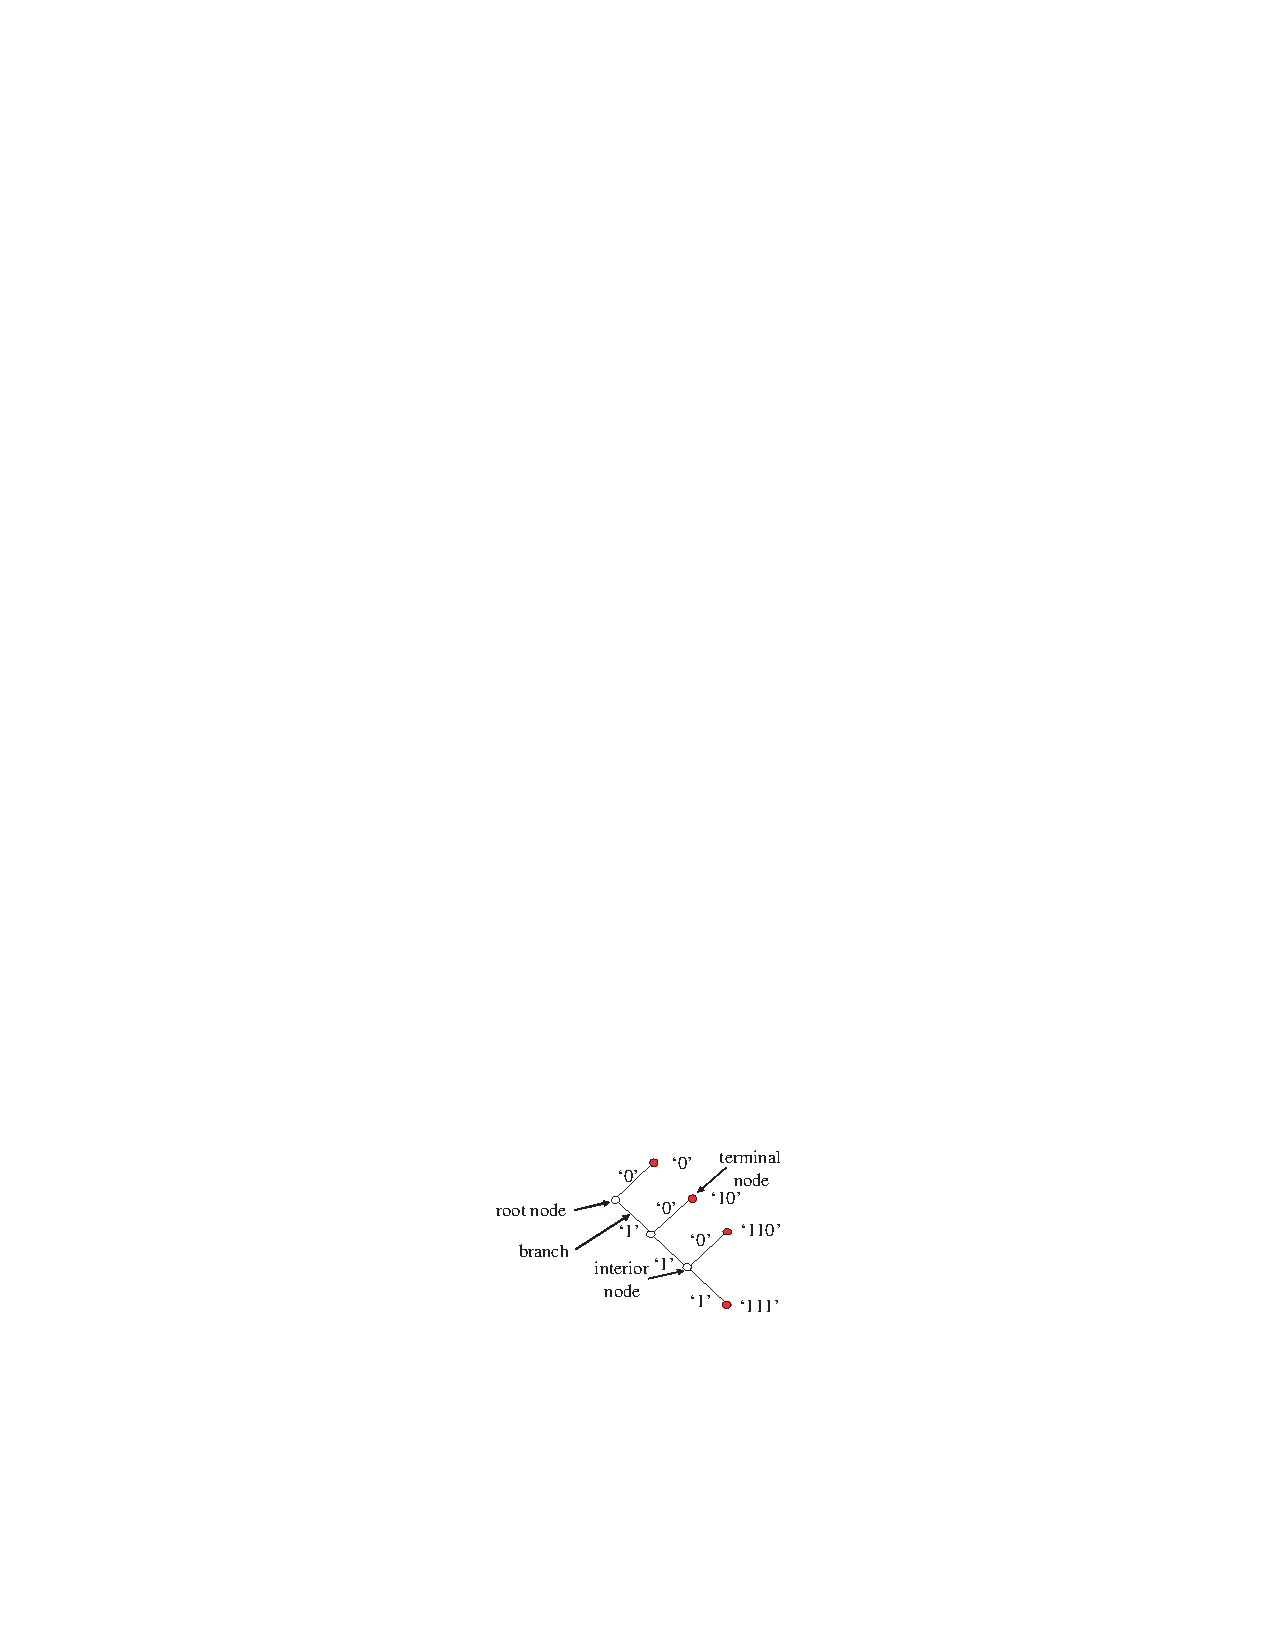
\includegraphics[width=0.5\textwidth]{Figures/PrefixCode}
\caption{Arbre binaire d'un code de $4$ symboles,
qui satisfait la condition de pr\'efixe. }
\label{prefixe6}
\end{figure}

Un code qui satisfait la condition de pr\'efixe peut \^etre
associ\'e \`a un arbre binaire, dont les $K$ feuilles correspondent
aux symboles $\{a_k \}_\UkK$.
Cette repr\'esentation est utile pour construire le code
qui minimise le nombre de bits moyen $R$.
Les branches de gauche et de droite de l'arbre binaire sont
respectivement cod\'ees par 0 et 1.
La figure \ref{prefixe6} montre un exemple pour un code
de $4$ symboles.
Le mot binaire $w_k$ associ\'e au symbole $a_k$
est la succession de $0$ et de $1$ correspondant aux branches
de gauche et de droite, le long du chemin de la racine de
l'arbre \`a la feuille correspondant \`a $a_k$.
Le code binaire g\'en\'er\'e par un tel arbre satisfait toujours
la condition de pr\'efixe. En effet, $w_m$ est
un pr\'efixe de $w_k$ si et seulement si
$a_m$ est un anc\^etre de $a_k$ dans l'arbre binaire.
Ceci n'est pas possible puisque les deux symboles correspondent
\`a des feuilles de l'arbre.
Inversement, tout code pr\'efixe peut \^etre repr\'esent\'e par un tel
arbre binaire.
La longueur $l_k$ du mot binaire
$w_k$ est la profondeur de la feuille $a_k$ dans l'arbre binaire.
L'optimisation d'un code de pr\'efixe est donc \'equivalente \`a
la construction d'un arbre binaire optimal qui distribue
les profondeur des feuilles de fa\c con \`a minimiser
(\ref{bit-rate}).

\subsection{Entropie de Shannon}
Le th\'eor\`eme de Shannon prouve que le nombre moyen de bit $R$
par symbole est plus grand que l'entropie.

\begin{theorem} [Shannon]
\label{shan-th}
On suppose que les symboles
$\{a_k\}_{1 \leq k \leq K}$ apparaissent avec la distribution
de probabilit\'e $\{p(a_k)\}_\UkK$.
Le nombre moyen $R$ de bit d'un code ayant la propri\'et\'e du
pr\'efixe satisfait
\begin{equation}
\label{shan1}
R \geq H = - \sum_{k=1}^K p(a_k) \log_2 p(a_k) .
\end{equation}
Il existe un code ayant la propri\'et\'e du pr\'efixe tel que
\begin{equation}
\label{shan2}
R \leq H + 1.
\end{equation}
\end{theorem}
\begin{proof}
Le th\'eor\`eme de Shannon se d\'emontre \`a partir de
l'in\'egalit\'e de Kraft.

\begin{lemma} [In\'egalit\'e de Kraft]
Tout code ayant la propri\'et\'e du pr\'efixe satisfait
\begin{equation}
\label{kraft}
\sum_{k=1}^K 2^{-l_k} \leq 1 .
\end{equation}
Inversement, si
$\{ l_k \}_\UkK$ sont des entiers positifs tels que
l'in\'egalit\'e (\ref{kraft}) est satisfaite alors il existe
un code de mots binaires $\{w_k \}_\UkK$ de longueurs
$\{ l_k \}_\UkK$ et qui satisfait la condition de pr\'efixe.
\end{lemma}

Pour d\'emontrer (\ref{kraft}) on associe un arbre binaire
au code consid\'er\'e. Chaque $l_k$ correspond \`a un noeud
de l'arbre \`a une profondeur $l_k$ qui d\'epend du mot
binaire $w_k$. Soit
\begin{equation}
\label{mmax}
m = \max \{l_1, l_2, \dots , l_K\} .
\end{equation}
On consid\'ere l'arbre binaire complet dont toutes les
feuilles sont \`a la profondeur $m$.
On note $T_k$ le sous-arbre issu du noeud correspondant au
mot binaire $w_k$. Ce sous arbre a une profondeur ${m - l_k}$
et contient donc $2^{m - l_k}$ noeud au niveau $m$.
Comme il y a $2^m$ noeud \`a la profondeur $m$ de l'arbre binaire
complet et que
la propri\'et\'e du pr\'efixe implique
que tous les sous arbres $T_1 , \dots , T_K$ sont distincts, on
d\'eduit que
\[
\sum_{k=1}^K 2^{m-l_k} \leq 2^m ,
\]
d'o\`u (\ref{kraft}).



Inversement, on consid\`ere $\{ l_k \}_\UkK$ satisfaisant
(\ref{kraft}) avec $l_1 \leq l_2 \leq \dots \leq l_K$ et
$m = \max \{l_1, l_2, \dots , l_K\}$.
On d\'efinit les ensembles $N_1$ des $2^{m-l_1}$ premiers
noeud au niveau $m$ sur la gauche de l'arbre, puis $N_2$
l'ensemble des $2^{m-l_2}$ noeuds suivants et ainsi de suite.
Les noeuds des ensembles $N_k$ sont les noeuds terminaux
de sous-arbres $T_k$ qui sont disjoints. On associe
\`a la racine de l'arbre $T_k$ qui est \`a la profondeur
$l_k$ le mot binaire $w_k$. Cela d\'efinit un code
qui satisfait la condition du pr\'efixe o\`u chaque
mot a la longueur $l_k$ voulue.
Cela termine la d\'emonstration du lemme.

Pour d\'emontrer les deux in\'egalit\'es (\ref{shan1}) et
(\ref{shan2}) du
th\'eor\`eme, on consid\`ere la minimisation de
\[
R = \sum_{k=1}^K p(a_k) \,l_k
\]
sous la contrainte de Kraft
\[
\sum_{k=1}^K 2^{-l_k} \leq 1 .
\]
Dans un premier temps, nous
supposons que $l_k$ peut \^etre un r\'eel quelconque.
Le minimum se calcule en utilisant un multiplicateur de
Lagrange $\lambda$ et en minimisant
\[
J = \sum_{k=1}^K p(a_k) l_k + \lambda \sum_{k=1}^K 2^{-l_k} .
\]
L'annulation de la d\'erivee par rapport \`a $l_k$ donne
\[
\frac {\partial J} {\partial l_k} = p(a_k) - \lambda \,2^{-l_k}\,
\log_{\exp} 2  = 0 .
\]
Le minimum est obtenu pour $\sum_{k=1}^K 2^{-l_k} = 1$
et comme $\sum_{k=1}^K p(a_k) = 1$ on obtient
$\lambda = 1/\log_{\exp} 2$. La longueur optimale minimisant
$R$ est donc
\[
l_k = -\log_2 p(a_k) ,
\]
et
\[
R =
\sum_{k=1}^K p(a_k)\, l_k = - \sum_{k=1}^K p(a_k) \log_2 p(a_k) = H .
\]

Pour garantir que $l_k$ est entier, on choisit
\[
l_k = \lceil - \log_2 p(a_k) \rceil
\]
o\`u $\lceil x \rceil$ est la plus petite valeur enti\`ere
sup\'erieure \`a $x$.
Cela correspond au code de Shannon.
Comme $l_k \geq - \log_2 p(a_k)$, l'in\'egalit\'e
de Kraft est satisfaite puisque
\[
\sum_{k=1}^K 2^{-l_k} \leq \sum_{k=1}^K 2^{\log_2 p(a_k)} = 1 .
\]
Il existe donc un code pr\'efixe dont les mots de code
ont une longueur $l_k$. Pour ce code
\[
\sum_{k=1}^K p(a_k) l_k \leq
\sum_{k=1}^K p(a_k) (-\log_2 p(a_k) + 1) = H + 1 .
\]
\end{proof}

\subsection{Codage par blocs}
L'ajout de 1 bit dans l'in\'egalit\'e (\ref{shan2})
vient du fait que $-\log_2 p_i$ n'est pas n\'ecessairement
un entier alors que la longueur d'un mot binaire doit
\^etre un entier. On peut construire des codes tels que
$R$ est plus proche de $H$ en r\'epartissant ce bit
suppl\'ementaire sur un bloc de $n$ \'el\'ements.
Au lieu de faire un codage instantan\'e, symbole par symbole,
on code d'un coup le bloc de symboles
$\vec X = X_1 , \,\dots\,,X_n$, qui peut \^etre consid\'er\'e
comme une variable al\'eatoire \`a valeurs dans
l'alphabet $A^n$ de taille $K^n$.
A tout bloc de symboles $\vec a \in A^n$ on associe un
mot binaire de longuer $l(\vec a)$. Le nombre de bits
$R$ par symbole pour un tel code par bloc est
\[
R = \frac 1 n \sum_{\vec a \in A^n} p(\vec a) \, l(\vec a) .
\]


\begin{proposition}
\label{shan-prop}
Le nombre moyen $R$ de bit d'un code
par bloc de taille $n$ ayant la propri\'et\'e du
pr\'efixe satisfait
\begin{equation}
\label{shan12}
R \geq H = - \sum_{k=1}^K p(a_k) \log_2 p(a_k) .
\end{equation}
Il existe un code par blocs de taille
$n$ ayant la propri\'et\'e du pr\'efixe tel que
\begin{equation}
\label{shan22}
R \leq H + \frac 1 n.
\end{equation}
\end{proposition}
\begin{proof}
L'entropie associ\'ee \`a $\vec X$ est
\[
\vec H = \sum_{\vec x \in A^n} p(\vec x) \, \log_2 p(\vec x) .
\]
Comme les variables al\'eatoires $X_i$ sont ind\'ependantes
\[
p(\vec x) = p(x_1, \dots , x_n) = \prod_{i=1}^n p(x_i)~.
\]
On d\'emontre par r\'ecurrence sur $n$ que
$\vec H = n H$. Soit $\vec R$ le nombre de bits moyen
pour coder les $n$ symboles $\vec X$. Le th\'eor\`eme
de Shannon \ref{shan-th} montre que $\vec R \geq \vec H$
et qu'il existe un code par bloc tel que
$\vec R \leq \vec H + 1$. On d\'eduit donc
(\ref{shan12},\ref{shan22}) pour $R = \frac{\vec R} n$, qui
est le nombre de bits moyen par symbole.
\end{proof}

Ce th\'eor\`eme d\'emontre que des codes par blocs
utilisent un nombre moyen de bits par symbole qui tendent
vers l'entropie lorsque la taille du bloc augmente.

\subsection{Code de Huffman}
L'algorithme de Huffman est un algorithme de programmation dynamique
qui construit de bas en haut un arbre correspondant \`a un
code pr\'efixe et qui
minimise
\begin{equation}
\label{Rmoyen}
R = \sum_{k=1}^K p(a_k) \, l_k .
\end{equation}
Nous ordonnons
$\{a_k \}_\UkK$ pour que $p(a_k) \leq p(a_{k+1})$.
Pour minimiser (\ref{Rmoyen})
les symboles de plus petites probabilit\'es doivent \^etre
associ\'es aux mot binaires $w_k$ de longueur maximale, ce qui
correspond \`a un noeud au bas de l'arbre.
Nous commen\c cons donc par repr\'esenter les deux symboles de plus
petite probabilit\'e
$a_1$ et $a_2$ comme les enfants d'un noeud commun.
Ce noeud peut \^etre interpr\'et\'e comme un symbole
$a_{1,2}$ correspondant \`a ``$a_1$ ou $a_2$'' et
dont la probabilit\'e est
$p(a_1) + p(a_2)$. La proposition suivante prouve que
l'on peut it\'erer ce regroupement \'el\'ementaire et construire un
code optimal.

\begin{proposition}
On consid\`ere $K$ symboles avec leurs probabilit\'es
ordonn\'ees en ordre croissant: $p(a_k) \leq p(a_{k+1})$.
On regroupe les deux symboles $a_1$ et $a_2$ de probabilit\'e
minimum en un seul symbole $a_{1,2}$ de probabilit\'e
\[
p(a_{1,2}) = p(a_1) + p(a_2) .
\]
Un arbre correspondant \`a un code pr\'efixe optimal pour
les $K$ symboles se construit \`a partir
d'un arbre de code pr\'efixe optimal pour les $K-1$ symboles
$\{a_{1,2}\} \cup \{ a_k \}_{3 \leq k \leq K}$,
en divisant la feuille de
$a_{1,2}$ en deux noeuds correspondant \`a $a_1$ et $a_2$.
\end{proposition}

La d\'emonstration de cette proposition se trouve dans
\cite{bremaud-proba}.

Cette proposition r\'eduit la construction d'un code optimal de
$K$ symboles \`a la construction
d'un code optimal pour les $K-1$ symboles.
Le code de Huffman it\`ere $K-1$ fois
ce regroupement et fait progressivement pousser l'arbre
d'un code de pr\'efixe optimal depuis le bas jusqu'en haut.
Le Th\'eor\`eme \ref{shan-th} de Shannon prouve que
\begin{equation}
\label{entropy-bound}
H \leq R  \leq H + 1 .
\end{equation}
\\
\\
\subsection{Exemple}
Les probabilit\'es des $\{a_k\}_{1 \leq k \leq 6}$ sont
\begin{equation}
\label{proba-code}
\{p(a_k)\}_{1 \leq k \leq 6} = \{0.05~,~0.1~,~0.1~,~0.15~,~0.2~,~0.4\}.
\end{equation}

La figure \ref{arbre-binaire}
donne l'arbre binaire construit avec l'algorithme
de Huffman.
Les symboles $a_1$ et $a_2$ sont regroup\'es
en un symbole $a_{1,2}$
de probabilit\'e $p(a_{1,2}) = p(a_1)+p(a_2)= 0.15$. A l'it\'eration suivante,
les symboles de plus basse probabilit\'e sont
$p(a_3) = 0.1$ et $p(a_{1,2}) = 0.15$. On regroupe donc
$a_{1,2}$ et $a_3$ en un symbole $a_{1,2,3}$ dont la probabilit\'e
est $0.25$. Les deux symboles de probabilit\'es les plus faibles sont
alors $a_4$ et
$a_5$ qui sont regroup\'es en $a_{4,5}$
de probabilit\'e $0.35$. On regroupe ensuite $a_{4,5}$ et
$a_{1,2,3}$ pour obtenir un symbole $a_{1,2,3,4,5}$ de probabilit\'e
$0.6$ qui est finalement regroup\'e avec $a_6$, ce qui finit
le code, comme l'illustre
l'arbre de la figure \ref{arbre-binaire}.
Le nombre moyen de bits obtenu par ce code est
$R= 2.35$ alors que l'entropie est $H = 2.28$.

\begin{figure}[bhtp]
\centerline{
        \epsfxsize=6cm
	\leavevmode\epsfbox{NewFig/fig3.eps}}
\caption {Arbre correspondant au code de Huffman pour une
source dont les probabilit\'es sont donn\'ees par
(\protect \ref{proba-code}) \protect \cite{vetterli}.}
\label{arbre-binaire}
\end{figure}
\\
\\
\noindent
\subsection{Sensibilit\'e au bruit}
Un code de Huffman est plus compact qu'un code de taille fixe
$\log_2 K$ mais est aussi plus sensible au bruit.
Pour un code de taille constante, une erreur
de transmission d'un bit modifie
seulement la valeur d'un symbole.
Au contraire, une erreur d'un bit
dans un code de taille variable peut modifier toute la suite
des symboles.
Lors de transmissions bruit\'ees, de telles erreurs peuvent se
produire. Il est alors n\'ecessaire d'utiliser un code correcteur
qui introduit une l\'eg\`ere redondance de facon \`a identifier les
erreurs.

\section{Quantification scalaire}
\label{scalar-quant-sec}

Si une variable al\'eatoire $X$
prend des valeurs r\'eelles quelconques, on ne peut pas
obtenir un code exact de taille finie.
Il est alors n\'ecessaire d'approximer $X$ par
$\tilde X$ qui prend ses valeurs dans un alphabet fini, et
l'erreur r\'esultante est
\[
D = E \{|X - \tilde X|^2\} .
\]
Un quantificateur scalaire d\'ecompose l'axe r\'eel en
$K$ intervalles $\{[y_{k-1} , y_k ]\}_{1 \leq k \leq K}$
de tailles variables, avec $y_0 = -\infty$ et $y_K = +\infty$.
Le quantificateur associe \`a tout
$x \in [y_{k-1} , y_k]$ une valeur
$Q(x) =a_k$.
Si les $K$ niveaux de quantification $\{a_k\}_{\UkK}$
sont fix\'es a priori,
pour minimiser $|x - Q(x)| = |x - a_k|$,
il faut que la quantification
associe \`a $x$ son niveau de quantification $a_k$ le plus
proche. On doit alors choisir des intervalles de quantification
qui satisfont
\begin{equation}
\label{opt-interv}
y_k = \frac {a_k + a_{k+1}} 2
\end{equation}
\\
\\
\subsection{Quantification haute r\'esolution}
Soit $p(x)$ la densit\'e de probabilit\'e de $X$.
On note $\tilde X = Q (X)$ la variable quantifi\'ee.
L'erreur quadratique moyenne est
\begin{equation}
\label{quantize-error}
D = E\{(X- \tilde X)^2\} =
\int_{-\infty}^{+\infty} |x - Q(x)|^2 p(x) dx .
\end{equation}

On dit que le quantificateur a une haute
r\'esolution si
$p(x)$ peut \^etre approxim\'e par une constante sur tout intervalle
de quantification $[{y_{k-1}},{y_{k}}]$.
La taille de ces intervalles est $\Delta_k = y_k - y_{k-1}$.
L'hypoth\`ese de haute r\'esolution implique que
\begin{equation}
\label{high-resol-quant}
p(x) = \frac {p_k} {\Delta_k} ~~\mbox{pour $x \in [y_{k-1},{y_{k}}]$},
\end{equation}
avec
\[
p_k = \PP \{X \in [{y_{k-1}},y_{k}] \} = \PP \{ \tilde X = a_k \} .
\]
La proposition suivant calcule l'erreur $D$ sous cette hypoth\`ese.

\begin{proposition}
Pour un quantificateur de haute r\'esolution sur des intervalles
$[{y_{k-1}},{y_{k}}]$, l'erreur $D$
minimum obtenue en optimisant la position des niveaux
$\{ a_k \}_{0 \leq k \leq K}$ est
\begin{equation}
\label{quadr-error}
D = \frac 1 {12} \sum_{k=1}^{K} {p_k} \, {\Delta_k ^2} .
\end{equation}
\end{proposition}
\begin{proof}
Comme $Q(x) = a_k$ si
$x \in [y_{k-1},y_k)$, on peut re\'ecrire (\ref{quantize-error})
\[
D = \sum_{k=1}^{K} \int_{y_{k-1}}^{y_{k}} (x - a_k)^2 p(x) dx .
\]
En rempla\c{c}ant $p(x)$ par son expression
(\ref{high-resol-quant}) on a
\begin{equation}
D =
\sum_{k=1}^{K} \frac {p_k} {\Delta_k}
\int_{y_{k-1}}^{y_{k}} (x - a_k)^2  dx.
\end{equation}
Cette erreur est minimum
pour $a_k = \half (y_{k}+{y_{k-1}})$, et l'int\'egration donne
(\ref{quadr-error}).
\end{proof}

\subsection{Quantification uniforme}
Le quantificateur uniforme est un cas particulier important o\`u
tous les intervalles de quantification sont de m\^eme taille
\[
y_{k} - y_{k-1} = \Delta ~~~\mbox{pour $1 \leq k \leq K$} .
\]
L'erreur quadratique moyenne (\ref{quadr-error})
devient
\begin{equation}
\label{unifoquantiz}
D = \frac {\Delta^2} {12} \sum_{k=1}^{K} {p_k}
= \frac {\Delta^2} {12} .
\end{equation}
Elle est ind\'ependante de la distribution de probabilit\'e
$p(x)$ de la source.
\\
\\
\subsection{Quantification optimale}
On veut optimiser
le quantificateur pour minimiser le nombre de bits
n\'ecessaires pour coder les valeurs quantifi\'ees
$\tilde X$, \'etant donn\'ee une distortion $D$ admissible.
Le th\'eor\`eme de
Shannon \ref{shan-th} prouve que la valeur moyenne minimum de bits
n\'ecessaire pour coder $\tilde X$ est sup\'erieure \`a l'entropie $H$
de la variable al\'eatoire $\tilde X$.
Comme le
code de Huffman donne un r\'esultat proche de cette entropie,
il nous faut minimiser l'entropie $H$ pour $D$ fixe.

La source quantifi\'ee $\tilde X$ prend $K$ valeurs diff\'erentes
$\{a_k\}_{1 \leq k \leq K}$ avec probabilit\'es
$\{p_k\}_{1 \leq k \leq K}$.
L'entropie du signal quantifi\'e est donc
\[
H = - \sum_{k=1}^K p_k\, \log_2 p_k .
\]
On d\'efinit l'entropie diff\'erentielle de la variable al\'eatoire
$X$ \`a valeurs r\'eelles
\begin{equation}
\label{entropie-dffD}
H_d = - \int_{-\infty}^{+\infty} p(x) \log_2 p(x) dx .
\end{equation}
Le th\'eor\`eme suivant montre que pour un quantificateur de haute
r\'esolution produisant une erreur $D$,
l'entropie est minimum lorsque le quantificateur est
uniforme.

\begin{theorem}
\label{quanti-theo}
L'entropie de
tout quantificateur de haute r\'esolution satisfait
\begin{equation}
\label{lower-quantX}
H \geq H_d - \frac 1 2 \log_2 (12 D) .
\end{equation}
Le minimum est atteint si et seulement si $Q$ est un
quantificateur uniforme.
\end{theorem}
\begin{proof}
Pour un quantificateur de haute r\'esolution
$p(x)$ est approximativement constant sur $[y_{k-1},y_k]$
et donc
\[
p_k = \int_{y_{k-1}}^{y_k} p(x)\,dx = p_k \Delta_k
\]
avec $\Delta_k = y_k - y_{k-1}$.
Donc
\begin{eqnarray*}
H & = & - \sum_{k=1}^K p_k \log_2 (p(a_k)\, \Delta_k )\\
& = &- \sum_{k=1}^K \int_{y_{k-1}}^{y_k} p(x) \log_2 p(a_k)\, dx
- \sum_{k=1}^K p_k \log_2 \Delta_k \\
& = & H_d - \frac 1 2 \sum_{k=1}^K p_k \log_2 \Delta_k^2 ,
\end{eqnarray*}
car $p(x) = p(a_k)$ pour $x \in [y_{k-1},y_k]$.
Pour toute fonction concave $\phi (x)$, l'in\'egalit\'e de Jensen
montre que pour tout $\sum_{k=1}^K p_k = 1$
et $\{a_k \}_\UkK$ alors
\begin{equation}
\label{jensen}
\sum_{k=1}^N p_k \phi ( a_k) \leq \phi(\sum_{k=1}^N  p_k a_k) .
\end{equation}
Si $\phi (x)$ est strictement concave, l'in\'egalit\'e devient une \'egalit\'e
si et seulement si tous les $a_k$ sont \'egaux lorsque
$p_k \neq 0$. Comme $\log_2(x)$ est strictement concave,
(\ref{quadr-error}) montre que
\[
 \frac 1 2 \sum_{k=1}^N p_k \log_2 \Delta_k^2 \leq
 \frac 1 2 \log_2 \sum_{k=1}^N p_k \Delta_k^2 =
 \frac 1 2 \log_2 (12 D ) .
\]
On en d\'eduit donc que
\[
H \geq H_d - \frac 1 2 \log_2 (12 D ).
\]
Cette in\'egalit\'e devient une \'egalit\'e si et seulement si tous les
$\Delta_k$ sont \'egaux, ce qui correspond \`a un quantificateur
uniforme.
\end{proof}
Ce th\'eor\`eme montre que pour un quantificateur haute r\'esolution
le nombre minimum de bits
$R = H$ est obtenu pour un quantificateur uniforme et
\begin{equation}
\label{bit-rate-uniform}
R = H_d -  \frac 1 2 \log_2 (12 D ).
\end{equation}
La distortion en fonction du nombre de bits est donc
\[
D(R) = \frac 1 {12}\, 2^{2 H_d} \,2^{-2R} .
\]

\chapter{Application au codage de parole}
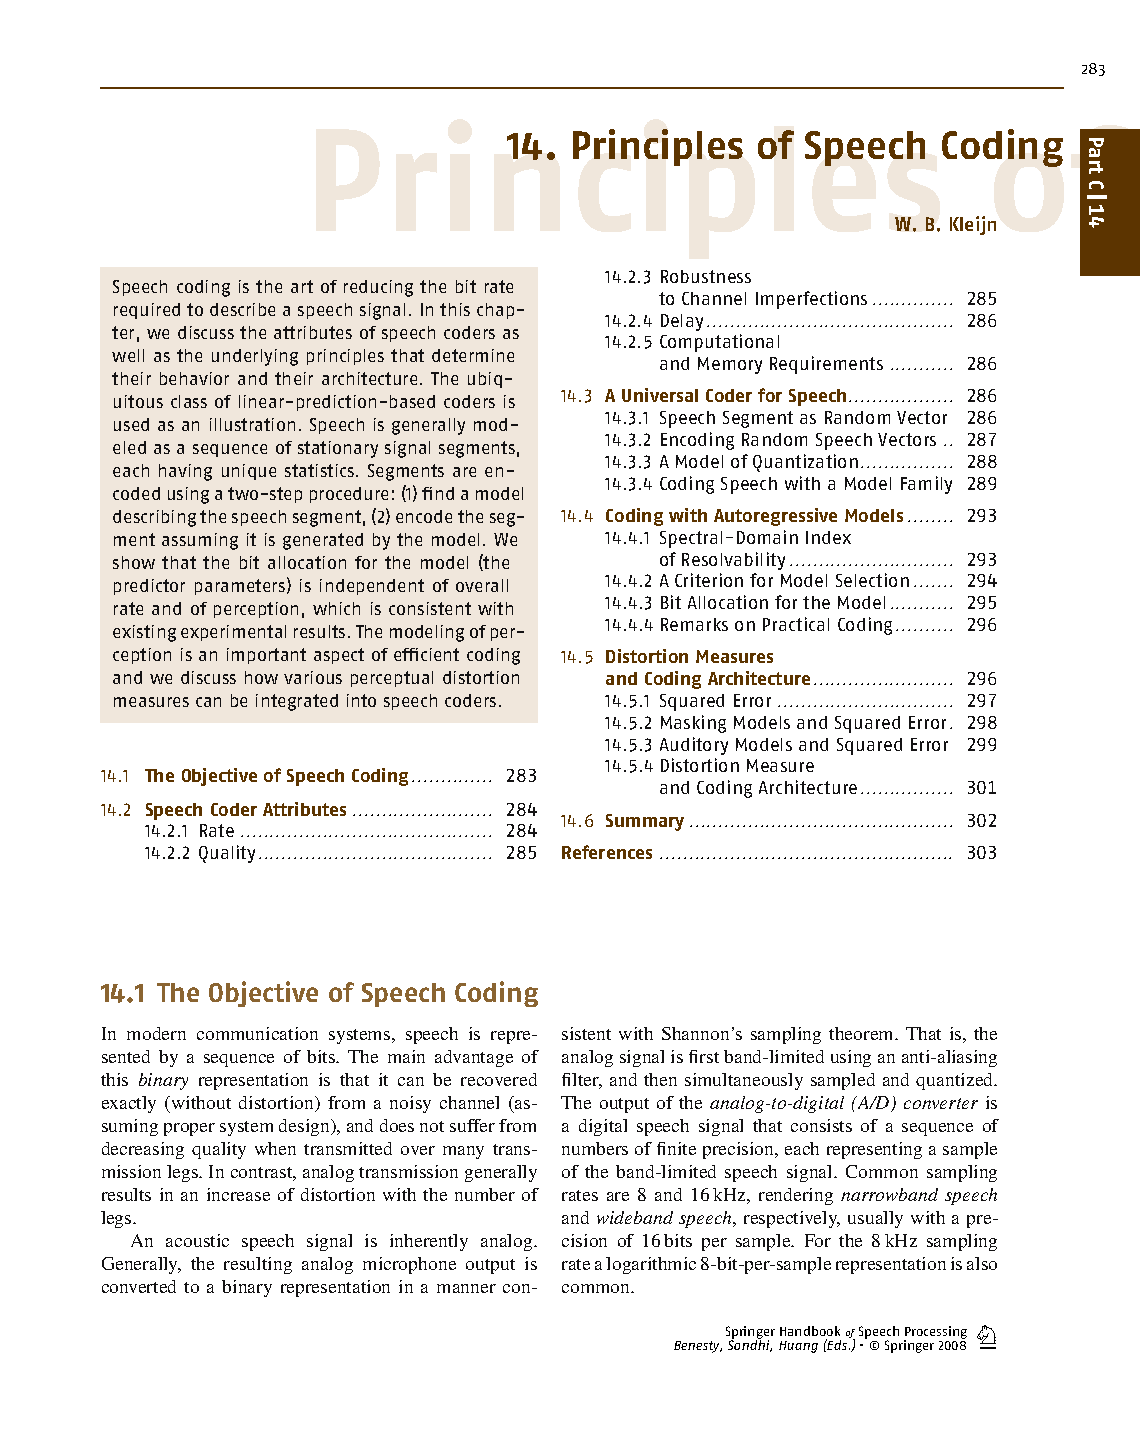
\includepdf[pages=-]{SpeechCoding}
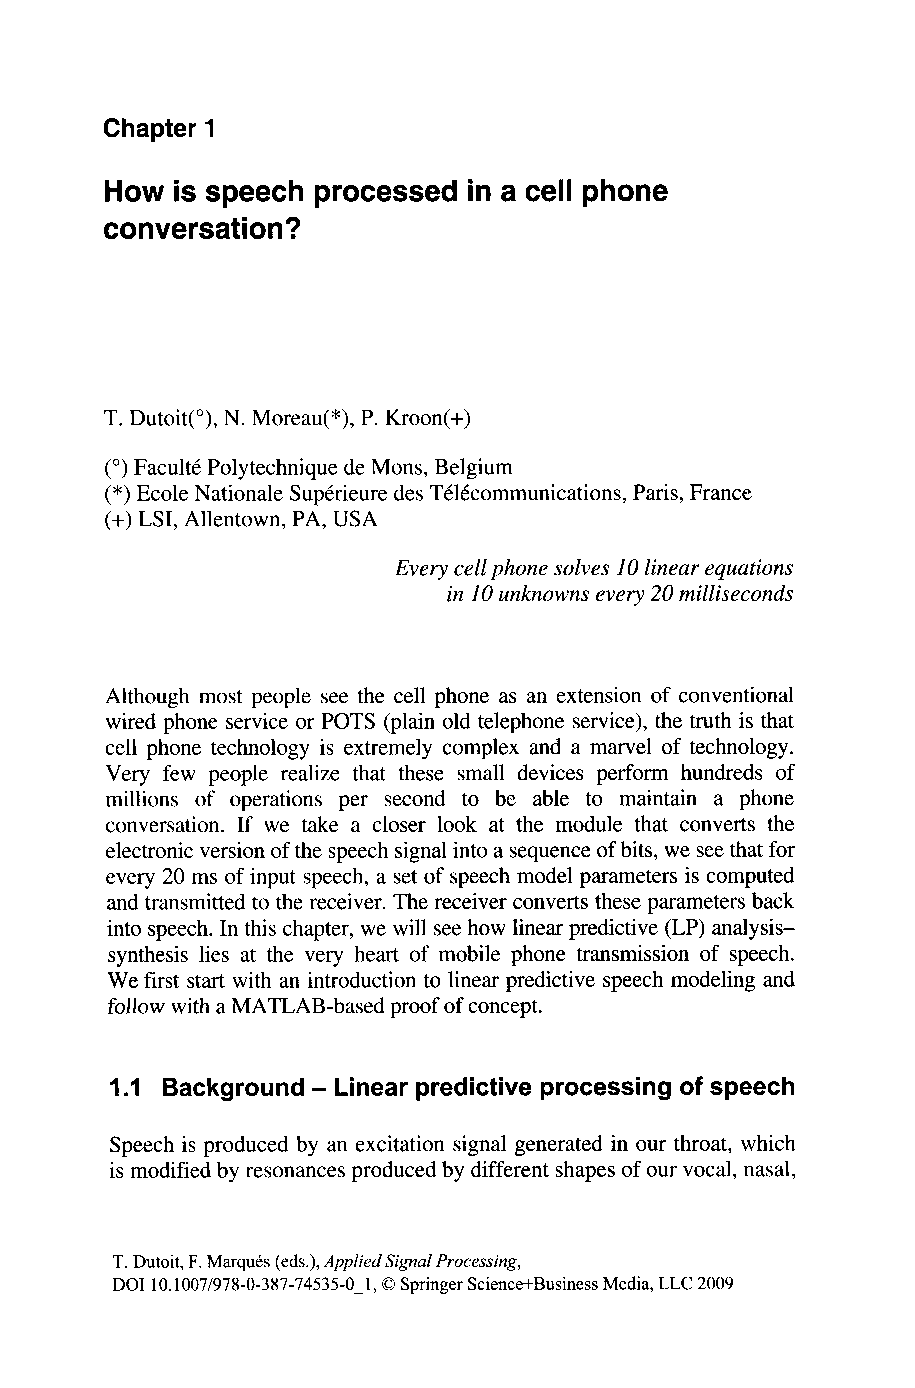
\includepdf[pages=-]{Vocoder}
\chapter{Application au codage d'images}
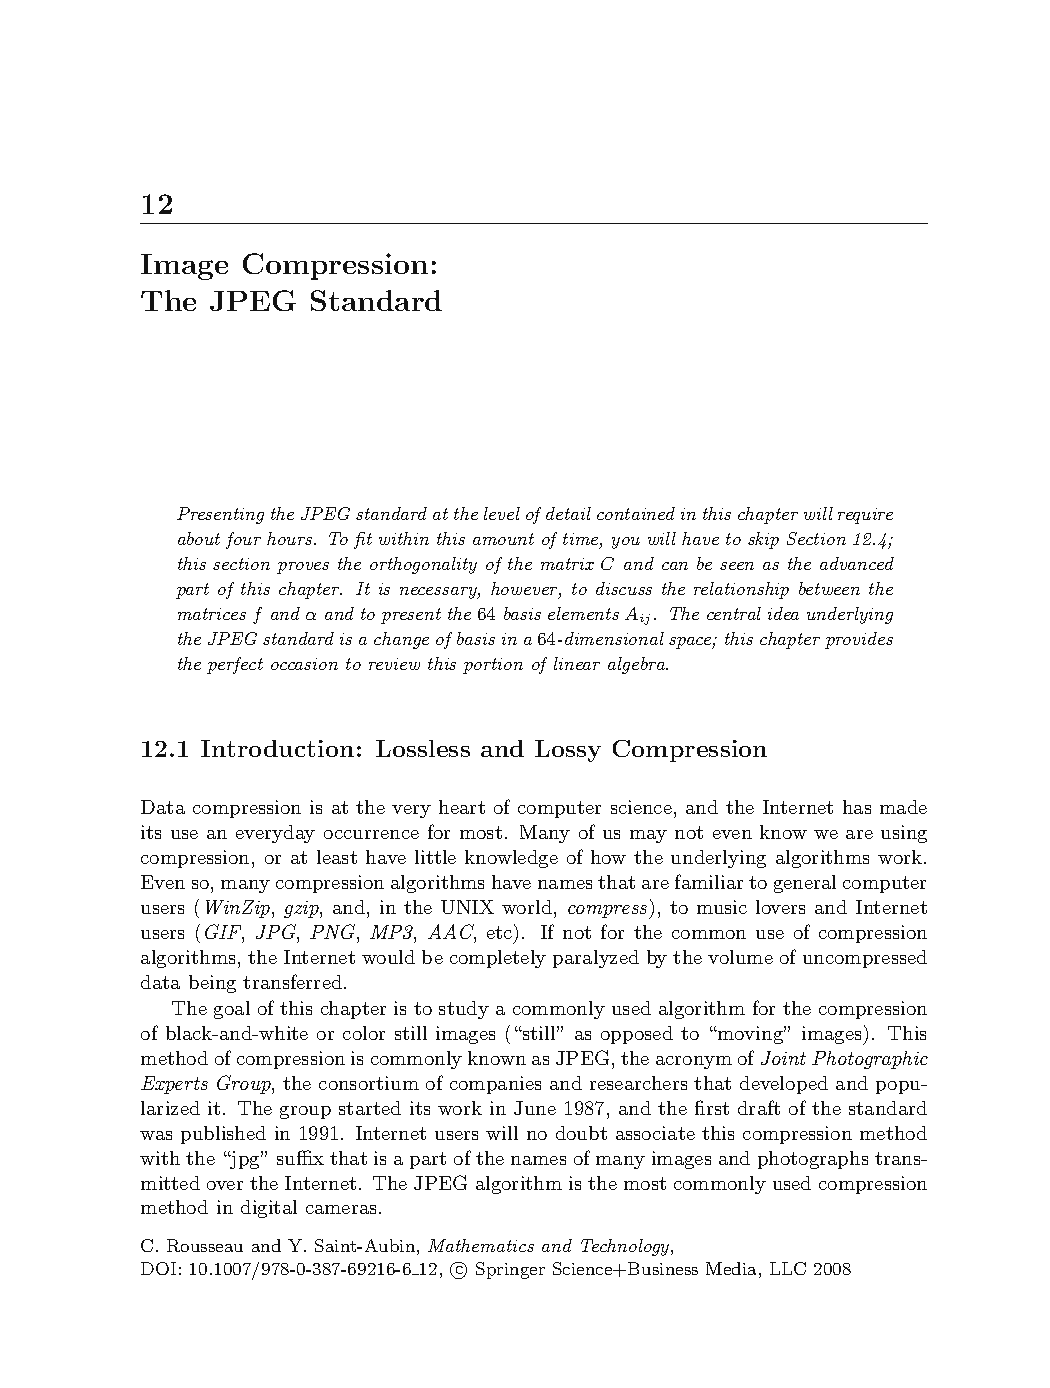
\includepdf[pages=-]{ImageCompression}
\begin{thebibliography}{99}

\bibitem{bremaud} P. Br\'emaud,
``Signaux al\'eatoires pour le traitement du signal et les communications'',
{\em Collection: Cours de l'Ecole Polytechnique, Ellipses}, 1993.

\bibitem{bremaud-proba} P. Br\'emaud,
``Introduction aux probabilit\'es'', Springer Verlag, Berlin.

\bibitem{bony} J.M. Bony,
``Cours d'Analyse'',
{\em Ecole Polytechnique}, 1994.

\bibitem{bony2} J.M. Bony,
``M\'ethodes math\'ematiques pour les sciences physiques,''
{\em Ecole Polytechnique}, 1995.

\bibitem{genat} J.F. Genat,
``Synth\`ese et traitement des sons en temps r\'eel'',
{\em Ecole Polytechnique}, 1994.

\bibitem{karar} J.F Genat et A. Karar,
``Introduction \`a l'analyse et synth\`ese de la parole'',
{\em Ecole Polytechnique}, 1994.

\bibitem{haykin} S. Haykin,
``Adaptive filter theory'',
{\em Prentice Hall}, 1991.

\bibitem{neveu} J. Neveu,
``Introduction aux Probabilit\'es'',
{\em Ecole Polytechnique}, 1994.

\bibitem{oppenheim} A. Oppenheim et R. Schafer,
``Discrete-time signal processing'',
{\em Prentice Hall}, 1989. 

\bibitem{parson} T. Parsons,
``Voice and speech processing'',
{\em Mc-Graw Hill}, 1987.

\bibitem{pap} A. Papoulis,
``Signal analysis'',
{\em Mc Graw Hill}, 1977.

\bibitem{priest} M.B. Priestley,
``Spectral analysis and time series'',
{\em Academic Press}, 1981.

\bibitem{thomas} Y. Thomas,
``Signaux et syst\`emes lin\'eaires'',
{\em Masson}, 1994.

\bibitem{torresani} B. Torr\'esani,
``Analyse continue par ondelettes'',
{\em CNRS editions}, {1995}.

\bibitem{vetterli} M. Vetterli and J. Kovacevic, 
``Wavelets and subband coding'',
{\em Prentice Hall}, 1995.

\end{thebibliography}
\appendix
\part{Compl\'ements math\'ematiques}
\chapter{Bases d'analyse Hilbertienne}
\chapter{Bases d'analyse Hilbertienne}
Ce chapitre n'est pas un cours d'analyse Hilbertienne, mais
rassemble les notions essentielles que nous aurons \`{a} manipuler dans ce
cours. La plupart des r\'{e}sultats sont \'{e}l\'{e}mentaires et sont d\'{e}montr\'{e}s.
%====================================================================
%================================================
%================================================
\section{D\'{e}finitions}
\begin{definition}[Espace pr\'{e}-hilbertien]
\label{def:prod_inter} Soit $\mathcal{H}$ un espace vectoriel sur
l'ensemble des nombres complexes $\Cset$. L'espace $\mathcal{H}$
est appel\'{e} \emph{pr\'{e}-hilbertien} si $\mathcal{H}$ est muni d'un
produit scalaire\,:
$$
 \pscal{\cdot}{\cdot}\, : x,y\in \mathcal{H} \times \mathcal{H}
 \mapsto \pscal{x}{y}\in \Cset
$$
qui v\'{e}rifie les propri\'{e}t\'{e}s suivantes\,:
\begin{enumerate}[label=\emph{\alph*})]
   %===
\item pour tout $(x,y) \in \mathcal{H} \times \mathcal{H}$,
  $\pscal{x}{y}=\overline{\pscal{y}{x}}$
   %===
   \item pour tout $(x,y) \in \mathcal{H} \times \mathcal{H}$ et tout $(\alpha,\beta) \in \Cset \times \Cset$,
$\pscal{\alpha x+ \beta y}{z}= \alpha \pscal{x}{z}+ \beta \pscal{y}{z}$
   %===
   \item pour tout $x \in \mathcal{H}$, $\pscal{x}{x}\geq 0$, et $\pscal{x}{x}=0$ si et seulement si $x=0$.
\end{enumerate}
L'application\,:
\[
\| \centerdot \|\, : x\in\mathcal{H}
  \mapsto \sqrt{\pscal{x}{x}} \geq 0
\]
d\'{e}finit alors une norme sur $\mathcal{H}$.
\end{definition}
\begin{example}[Espace $\Cset^n$]
L'ensemble des vecteurs colonnes
$x=[\begin{matrix}x_1&\cdots&x_n\end{matrix}]^T$, o\`{u} $x_k\in
\Cset$, est un espace vectoriel dans lequel la relation\,:
% \footnote{Dans cet ouvrage, l'exposant $^H$ indique l'op\'{e}rateur de transposition
%     et conjugaison des matrices.}
$$
\pscal{x}{y}=y^Hx=\sum_{k=1}^n x_k\overline{y_k}
$$
d\'{e}finit un produit scalaire.
\end{example}
\begin{example}[Espace $\pltwo$]
L'ensemble des suites num\'{e}riques complexes $\{ x_k \}_{k \in
\nset}$ v\'{e}rifiant $\sum_{k = 0}^\infty |x_k|^2 < \infty$
est un espace vectoriel sur $\Cset$. On d\'{e}finit pour tout $x$ et $y$ de cet
espace\,:
\[
\pscal{x}{y} = \sum_{k=0}^\infty {x}_k\overline{y_k}
   \;.
\]
Cette somme est bien d\'{e}finie puisque $|{x}_k\overline{y_k}|\leq(|x_k|^2+|y_k|^2)/2$.
De plus, on v\'{e}rifie ais\'{e}ment les propri\'{e}t\'{e}s (i-iii) de la d\'{e}finition
\ref{def:prod_inter}. L'espace ainsi d\'{e}fini est donc un espace
pr\'{e}-Hilbertien, que l'on note $\pltwo$.
\end{example}
\begin{example}[Fonctions de carr\'{e} int\'{e}grable]
\label{exemple:L2}
  L'ensemble $\cL^2(T)$ des fonctions bor\'{e}liennes d\'{e}finies sur un intervalle
  $T$ de $\Rset$, \`{a} valeurs complexes et de module de carr\'{e} int\'{e}grable par
  rapport \`{a} la mesure de Lebesgue ($\int_T |f(t)|^2 dt < \infty$) est un espace
  vectoriel.  Consid\'{e}rons alors le produit int\'{e}rieur\,:
\[
   (f,g) \in \cL^2(T) \times \cL^2(T)
    \mapsto \pscal{f}{g}=\int_T f(t) \overline{g(t)} \rmd t
\]
Cette int\'{e}grale est bien d\'{e}finie puisque
$|{f(t)} \overline{g(t)}|\leq(|f(t)|^2+|g(t)|^2)/2$
et l'on montre ais\'{e}ment que les propri\'{e}t\'{e}s
(i) et (ii) de la d\'{e}finition \ref{def:prod_inter}. Par contre la
propri\'{e}t\'{e} (iii) n'est pas v\'{e}rifi\'{e}e puisque\,:
\[
 \pscal{f}{f}=0 \not\Rightarrow \forall t\in T\ f(t)=0
\]
En effet une fonction $f$ qui est nulle sauf sur un ensemble de
mesure nulle pour la mesure de Lebesgue, v\'{e}rifie $\pscal{f}{f}=0$.
L'espace $\cH$ muni du produit $(f,g)$ n'est donc pas un espace
pr\'{e}-Hilbertienne.
C'est pourquoi on d\'{e}finit l'ensemble $\ltwo(T)$ des classes d'\'{e}quivalence
de  $\cL^2(T)$ pour la \emph{relation d'\'{e}quivalence} d\'{e}finie par
l'\'{e}galit\'{e} presque partout entre deux fonctions. Par construction,
 $L^2(T)$ est alors un espace pr\'{e}-Hilbertien.
\end{example}
\begin{example}[Variables al\'{e}atoires de variance finie]
\label{exemple:L2Omega}
De fa\c{c}on similaire \`{a} l'exemple~\ref{exemple:L2}, pour tout espace de
probabilit\'{e} $(\Omega,\cF,\PP)$, on d\'{e}finit $\cH=\cL^2(\Omega,\cF,\PP)$
(not\'{e} $\cL^2(\Omega)$ s'il n'y a pas de confusion possible) comme l'ensemble
des v.a. $X$ d\'{e}finies sur  $(\Omega,\cF,\PP)$ \`{a} valeurs complexes telles que
$$
\PE{|X|^2}<\infty\;.
$$
Sur cet ensemble, on d\'{e}finit
$$
   (X,Y) \in \cL^2(\Omega)\times \cL^2(\Omega)
    \mapsto \pscal{X}{Y}=\PE{ X \overline{Y}}\;.
$$
Pour les m\^{e}mes raisons que dans l'exemple~\ref{exemple:L2}, on d\'{e}finit l'espace
pr\'{e}-Hilbertien $L^2(\Omega,\cF,\PP)$ (ou $L^2(\Omega)$) comme l'ensemble des
classes d'\'{e}quivalences de $\cL^2(\Omega)$ pour la relation d'\'{e}quivalence
d\'{e}finie par l'\'{e}galit\'{e} presque s\^{u}re entre deux v.a.
Cet exemple et l'exemple~\ref{exemple:L2} se g\'{e}n\'{e}ralisent en fait \`{a} tout espace
mesur\'{e} $(\Omega,\cF,\mu)$ en posant
$$
(f,g) \in \cL^2(\Omega,\cF,\mu)\times \cL^2(\Omega,\cF,\mu)
    \mapsto \pscal{f}{g}=\int f\, \overline{g} \;\rmd\mu \;.
$$
\end{example}

On montre ais\'{e}ment les propri\'{e}t\'{e}s suivantes\,:
\begin{theorem}

\label{theo:cauchyandco}
 Pour tout $x,y \in \mathcal{H}\times
\mathcal{H}$, nous avons\,:
\begin{enumerate}[label=\emph{\alph*})]
   %===
   \item In\'{e}galit\'{e} de Cauchy-Schwarz\index{Cauchy-Schwarz (In\'{e}galit\'{e} de)}:
     $|\pscal{x}{y}| \leq \|x\| \|y\|$,
   %===
   \item In\'{e}galit\'{e} triangulaire:
 $\left | \|x\|-\|y\| \right |\leq \| x - y \| \leq \| x \| + \| y\|$,
   %===
   \item Identit\'{e} du parall\'{e}logramme:
\[
\| x + y \|^2 + \| x-y\|^2 = 2 \|x\|^2 + 2 \|y\|^2
\]
\end{enumerate}
\end{theorem}
%%%%%%%%
\begin{definition}[Convergence forte dans $\calH$]
Soit $(x_n)$ une suite de vecteurs  et $x$ un vecteur d'un espace
pr\'{e}hilbertien $\calH$. On dit que $(x_n)$ tend fortement
vers $x$ si et seulement si $\|x_n-x\| \rightarrow 0$ quand
$n\rightarrow +\infty$. On note $x_n \rightarrow x$.
\end{definition}
\begin{proposition}
\label{prop:cvgceforte-implique-borne}
Si dans un espace de Hilbert la suite $x_n\rightarrow x$, alors
$(x_n)$ est born\'{e}e.
\end{proposition}
\begin{proof}\smartqed
D'apr\`{e}s l'in\'{e}galit\'{e} triangulaire, on a~:
$$
 \|x_n\|=\|(x_n-x)+x\|\leq \|x_n-x\|+\|x\|
$$

\end{proof}

\begin{definition}[Convergence faible dans $\calH$]
Soit $(x_n)$ une suite de vecteurs  et $x$ un vecteur d'un espace
pr\'{e}hilbertien $\calH$. On dit que $(x_n)$ tend faiblement
vers $x$ si et seulement si, pour tout $y \in \calH$, $\pscal{x_n}{y} \to \pscal{x}{y}$ quand $n \to \infty$.
On note $x_n \rightsquigarrow x$.
\end{definition}
\begin{theorem}
\label{theo:cvgcefaible-implique-forte}
Une suite $(x_n)$ fortement convergente converge aussi faiblement vers la m\^{e}me limite.
\end{theorem}
\begin{proof}\smartqed
Supposons que $(x_n)$ converge fortement vers $x$, $\lim_{n \to \infty} \| x_n-x\|=0$. Alors,
pour tout $y \in \calH$,
\[
\left| \pscal{x_n-x}{y} \right| \leq \| x_n - x \| \| y \| \to 0 \eqsp, \quad \text{quand} \quad n \to \infty \eqsp.
\]

\end{proof}
En g\'{e}n\'{e}ral, la convergence faible n'entra\^{i}ne pas la convergence forte.
Pour tout $y \in \calH$, l'application $\pscal{\cdot}{y}: \calH \to \cset$, $x \mapsto \pscal{x}{y}$ est une forme
lin\'{e}aire. Le th\'{e}or\`{e}me~\ref{theo:cvgcefaible-implique-forte} montre que cette forme lin\'{e}aire est continue.
\begin{theorem}[Continuit\'{e} du produit scalaire]
\label{theo:cont_prod_int} Soit $x_n \rightarrow x$ et $y_n
\rightarrow y$ deux suites convergentes de vecteurs d'un espace
pr\'{e}-hilbertien $\mathcal{H}$. Alors quand $n\rightarrow
+\infty$\,: $\pscal{x_n}{y_n} \rightarrow \pscal{x}{y}$. En particulier, si $x_n
\rightarrow x$, $\| x_n \| \rightarrow \|x\|$.
\end{theorem}
\begin{proof}\smartqed
D'apr\`{e}s l'in\'{e}galit\'{e} triangulaire puis l'in\'{e}galit\'{e} de Cauchy-Schwarz,
nous avons\,:
\begin{align*}
\pscal{x}{y}-\pscal{x_n}{y_n}
 &= \pscal{(x - x_n) + x_n}{ (y - y_n) + y_n} - \pscal{x_n}{y_n} \\
 &= \pscal{x-x_n}{y-y_n} + \pscal{x-x_n}{y_n}+ \pscal{x_n}{y-y_n} \\
 &\leq \|x_n-x\|\|y_n-y\|+\|x_n-x\|\|y_n\|+\|y_n-x\|\|x_n\|
\end{align*}
On conclut en utilisant la proposition~\ref{prop:cvgceforte-implique-borne} qui montre que
les suites $(x_n)$ et $(y_n)$ sont born\'{e}es.

\end{proof}


\begin{definition}[Suite de Cauchy]
  Soit $(x_n)$ une suite de vecteurs d'un espace vectoriel norm\'{e}
  $(\mathcal{H},\|\cdot\|)$. On dit que $(x_n)$ est une suite de Cauchy si et
  seulement si\,:
$$
\| x_n - x_m\| \rightarrow 0
$$
quand $n,m \rightarrow +\infty$.
\end{definition}
Notons qu'en vertu de l'in\'{e}galit\'{e} triangulaire toute suite
convergente est une suite de Cauchy. La r\'{e}ciproque est fausse\,:
une suite de Cauchy peut ne pas \^{e}tre convergente. Un
contre-exemple est donn\'{e} par l'exemple~\ref{exe:C2pi}.
\begin{definition}[Espace complet, espace de Hilbert]
  On dit qu'un espace vectoriel norm\'{e} $(\mathcal{H},\|\cdot\|)$ est
  \emph{complet} si toute suite de Cauchy d'\'{e}l\'{e}ments de cet espace converge
  dans cet espace. On dit $\mathcal{H}$ est un \emph{espace de Hilbert} si
  $\mathcal{H}$ est pr\'{e}-hilbertien et complet.
\end{definition}
\begin{proposition}[Suites normalement convergentes]
Un espace vectoriel norm\'{e} $(\mathcal{H},\|\cdot\|)$ est complet si et seulement
si toute s\'{e}rie normalement convergente est convergente.
\end{proposition}
Ce r\'{e}sultat classique, voir  \cite[proposition~5 du chapitre~6,
page~124]{royden:1988}, est utile pour montrer que les espaces $L^p$ sont complets.
\begin{example}[Espace de  suite]
L'espace $\pltwo$ est un espace de Hilbert. Soit $(a_n)$ une suite de Cauchy dans $\pltwo$. Si nous notons
\[
a_n= (a_{n,1}, a_{n,2}, \dots ) \eqsp,
\]
alors, pour tout $\epsilon > 0$, il existe $N$ tel que, pour tout $n,m \geq N$,
\begin{equation}
\label{eq:keyidentite}
\sum_{k=1}^\infty |a_{m,k}- a_{n,k}| \leq \epsilon^2 \eqsp,
\end{equation}
pour tout $n,m \geq N$. Fixons tout d'abord $k$. La relation pr\'{e}c\'{e}dente montre
que la suite $(a_{n,k})$ est une suite de Cauchy dans $\cset$.  Cette suite
converge donc vers $\alpha_k$. Nous notons $a = (\alpha_k)$. Nous allons
montrer que $a \in \pltwo$ et que $\lim_{n \to \infty}\|a_n -a \|= 0$. Comme
l'espace $\pltwo$ est stable par diff\'{e}rence, nous allons montrer que pour tout
$n$, $a_n -a \in \pltwo$.  Comme $a = a_n - (a_n-a)$ et $a_n \in \pltwo$, cette
propri\'{e}t\'{e} implique donc que $a \in \pltwo$.

En utilisant \eqref{eq:keyidentite}, nous avons pour tout $p \in \nset$, et tout $m,n \geq N$,
\[
\sum_{k=1}^p |a_{m,k} - a_{n,k} |^2 \leq \sum_{k=1}^\infty |a_{m,k} - a_{n,k}|^2 \leq \epsilon^2.
\]
Par cons\'{e}quent, pour tout $p \in \nset$ et tout $n \geq N$,  $\lim_{m \to \infty} \sum_{k=1}^p |a_{m,k} - a_{n,k} |^2 =
\sum_{k=1}^p |a_k - a_{n,k}|^2 \leq \epsilon^2$. En prenant, la limite en $p$, nous obtenons donc, pour tout $n \geq N$,
\[
\|a - a_n\|^2 = \sum_{k=1}^\infty |a_k - a_{n,k}|^2 \leq \epsilon^2,
\]
ce qui montre que $(a - a_n) \in \pltwo$. Comme $\epsilon$ est arbitraire, nous avons aussi $\lim_{n \to \infty} \|a - a_n\|= 0$.
\end{example}
\begin{proposition}[Espaces $L^2$]
  Pour tout espace mesurable $(\Omega,\cF,\mu)$, L'espace
  $L^2(\Omega,\cF,\mu)$(voir l'exemple~\ref{exemple:L2Omega}) des fonctions de
  carr\'{e} int\'{e}grable pour la mesure $\mu$ est un espace de Hilbert.
\end{proposition}
Un r\'{e}sultat plus g\'{e}n\'{e}ral sur les espaces $L^p$ est fourni par
\cite[proposition~6 du chapitre~6, page~126]{royden:1988}.
% \begin{definition}[Sous espace vectoriel]
% Un sous-espace $\mathcal{E}$ d'un espace vectoriel $\mathcal{H}$
% est un sous-ensemble de $\mathcal{H}$ tel que, pour tout $x,y \in
% \mathcal{E}$ et tout scalaire $\alpha,\beta$, $\alpha x+ \beta y
% \in \mathcal{E}$. Un sous-espace vectoriel est dit \emph{propre}
% si $\mathcal{E} \ne \mathcal{H}$.
% \end{definition}
\begin{definition}[Sous-espace ferm\'{e}]
Soit $\cal E$ un sous-espace d'un espace de Hilbert $\cal H$. On
dit que $\cal E$ est ferm\'{e}, si toute suite $(x_n)$ de $\cal E$,
qui converge, converge dans $\cal E$.
\end{definition}
\begin{example}[Sous-espace non--ferm\'{e}, espace non-complet]
 \label{exe:C2pi}
Soit $\mathcal{C}([-\pi,\pi])$ l'espace des fonctions continues
sur $[-\pi,\pi]$. Cet espace est un sous-espace de
l'espace de Hilbert $L^2([-\pi,\pi])$. Consid\'{e}rons la suite de fonctions\,:
\[
 f_n(x)= \sum_{k=1}^n \frac{1}{k} \cos(kx)
\]
Les fonctions $f_n(x)$, qui sont ind\'{e}finiment contin\^{u}ment
diff\'{e}rentiables,  appartiennent \`{a} $\mathcal{C}(-\pi,\pi)$.
Montrons que cette suite est une suite de Cauchy. En effet, pour
$m > n$, on a\,:
\[
  \| f_n - f_m \|^2 =
    \pi \sum_{k=n+1}^m \frac{1}{k^2} \longrightarrow 0
    \quad \mbox{quand} \quad (n,m) \rightarrow \infty
\]
D'autre part on montre ais\'{e}ment que la limite de cette suite
$f_\infty(x) = \sum_{k=1}^\infty k^{-1} \cos(kx)= \log
|\sin(x/2)|$ n'est pas continue et n'appartient donc pas \`{a}
$\mathcal{C}([-\pi,\pi])$.
Le sous-espace  $\mathcal{C}([-\pi,\pi])$ est donc un sous-espace vectoriel de
$L^2([-\pi,\pi])$ mais n'est pas ferm\'{e}. C'est donc aussi un espace
pr\'{e}-hilbertien qui n'est pas complet.
\end{example}
\begin{definition}[Sous espace engendr\'{e} par un sous-ensemble]
\label{def:espace-engendre}
Soit $\mathcal{X}$ un sous-ensemble de $\mathcal{H}$. Nous notons
$\lspan{\mathcal{X}}$ le sous-espace vectoriel des combinaisons lin\'{e}aires
finies d'\'{e}l\'{e}ments de $\mathcal{X}$ et $\cspan{\mathcal{X}}$ \emph{l'adh\'{e}rence}
de $\lspan{\mathcal{X}}$ dans $\mathcal{H}$, c'est-\`{a}-dire le plus petit
sous-ensemble ferm\'{e} de $\mathcal{H}$ contenant $\lspan{\mathcal{X}}$, ou encore
l'espace obtenu par l'ensemble $\lspan{\mathcal{X}}$ compl\'{e}t\'{e} de toute les
limites de suite d'\'{e}l\'{e}ments de $\lspan{\mathcal{X}}$.
\end{definition}
\begin{definition}[Orthogonalit\'{e}]
Deux vecteurs $x,y \in \mathcal{H}$ sont dit \emph{orthogonaux},
si $\pscal{x}{y}= 0$, ce que nous notons $x \perp y$. Si $\mathcal{S}$
est un sous-ensemble de $\mathcal{H}$, la notation $x \perp
\mathcal{S}$, signifie que $x \perp s$ pour tout $s \in
\mathcal{S}$. Nous notons $\mathcal{S}\perp\mathcal{T}$ si tout
\'{e}l\'{e}ment de $\mathcal{S}$ est orthogonal \`{a} tout \'{e}l\'{e}ment de
$\mathcal{T}$.
\end{definition}
Supposons qu'il existe deux sous-espaces $\mathcal{A}$ et
$\mathcal{B}$ tels que $\mathcal{H} = \mathcal{A} \oplus \mathcal{B}$,
dans le sens o\`{u}, pour tout vecteur $h \in \mathcal{H}$, il
existe $a \in \cA$ et $b \in \cB$, tel que $h= a + b$. Si en plus
$\cA \perp \cB$ nous dirons que $\cH$ est la \emph{somme
directe} de $\cA$ et $\cB$, ce que nous notons $\cH= \cA \oplusperp
\cB$.
\begin{definition}[Compl\'{e}ment orthogonal]
Soit ${\cal E}$ un sous-ensemble d'un espace de Hilbert $\cal H$.
On appelle ensemble orthogonal de ${\cal E}$, l'ensemble d\'{e}fini
par\,:
$$
 {\cal E}^{\perp}=\{x\in {\cal H}:
    \forall y\in {\cal E} \hspace{5pt} \pscal{x}{y}=0\}
$$
\end{definition}
\section{Famille orthogonale et orthonormal}
\begin{definition}[Famille orthogonale, orthonormale]
Soit $E$ un sous ensemble de $\calH$. On dit que $E$
est une famille orthogonale si et seulement si pour tout $(x,y) \in E \times E$,
$x \ne y$, $\pscal{x}{y}= 0$. Si de plus   $\|x\|=1$ pour tout $x \in E$, on
dira que $E$ est une famille orthonormale.
\end{definition}
Une famille orthogonale a la propri\'{e}t\'{e} remarquable que dans le d\'{e}veloppement de
la norme quadratique des combinaisons lin\'{e}aires finies, les termes de doubles
produits sont nuls. Soit $E$ une famille orthogonale, $(x_1,\dots,x_n) \in E^n$
et $(\alpha_1,\dots,\alpha_n) \in \cset^n$. Alors
\begin{equation}
  \label{eq:norme_comb_lin_ortho}
\left\|\sum_{k=1}^n\alpha_k x_k\right\|^2= \sum_{k=1}^n |\alpha_k|^2
\|x_k\|^2\;.
\end{equation}
Il s'en suit donc le th\'{e}or\`{e}me \'{e}l\'{e}mentaire suivant.
\begin{theorem}
  Toute famille orthogonale d'\'{e}l\'{e}ments non-nuls est libre.
\end{theorem}
La relation~(\ref{eq:norme_comb_lin_ortho}) est bien connue en g\'{e}om\'{e}trie
euclidienne. L'avantage du cadre hilbertien est qu'il permet d'obtenir des
r\'{e}sultats pour une somme infinie.
\begin{theorem}
\label{theo:convergence-series-fourier}
Soit $(e_i)_{i\geq1}$ une suite orthonormale d'un espace de Hilbert $\calH$ et
soit $(\alpha_i)_{i\geq1}$ une suite de nombre complexes. La s\'{e}rie
\begin{equation}
  \label{eq:serie_suite_ortho}
  \sum_{i=1}^\infty  \alpha_i e_i
\end{equation}
converge dans $\calH$ si et seulement si $\sum_{i} |\alpha_i|^2 <
\infty$ auquel cas
\begin{equation}
  \label{eq:norm_serie_suite_ortho}
\left\| \sum_{i=1}^\infty \alpha_i e_i \right\|^2 =
\sum_{i=1}^\infty |\alpha_i|^2 \eqsp.
\end{equation}
\end{theorem}
\begin{proof}\smartqed
Pour tout $m > k > 0$, de m\^{e}me que pour
l'\'{e}quation~(\ref{eq:norme_comb_lin_ortho}), nous avons
\[
\left\| \sum_{i=k}^m \alpha_i e_i \right\|^2 = \sum_{i=k}^m |\alpha_i|^2 \eqsp.
\]
Comme $\sum_{i=1}^\infty |\alpha_i|^2 < \infty$, la suite $s_m= \sum_{i=1}^m
\alpha_i e_i$ est une suite de Cauchy dans $\calH$. Comme $\calH$ est complet,
cette suite de Cauchy converge. L'identit\'{e}~(\ref{eq:norm_serie_suite_ortho})
est obtenue par passage \`{a} la limite.

R\'{e}ciproquement, si la s\'{e}rie $\sum_{i=1}^\infty \alpha_i e_i$ converge, ce
passage \`{a} la limite reste valide
et~(\ref{eq:norm_serie_suite_ortho}) montre que la s\'{e}rie de terme
$(|\alpha_i|^2)_{i\geq1}$ est convergente.

\end{proof}
La question se pose aussi de savoir comment approcher un \'{e}l\'{e}ment $x$ de $\calH$
par une d\'{e}composition en s\'{e}rie de la forme~(\ref{eq:serie_suite_ortho}).
Pour cela le r\'{e}sultat suivant pour une famille finie sera utile.
\begin{proposition}
\label{prop:bessel}
Si $x$ est un vecteur d'un espace de Hilbert $\calH$ et si
$E=\{e_1,\cdots,e_n\}$ est une famille orthonormale finie, alors\,:
\begin{equation}
  \label{eq:famille_orthonorm_finie}
\left\| x-\sum_{k=1}^n \pscal{x}{e_k} e_k \right\|^2= \|x\|^2 - \sum_{k=1}^n |\pscal{x}{e_k}|^2\;.
\end{equation}
De plus
$\sum_{k=1}^n \pscal{x}{e_k} e_k$ est l'\'{e}l\'{e}ment de
$\lspan{e_1,\dots,e_n}$ le plus proche de $x$: la
quantit\'{e}~(\ref{eq:famille_orthonorm_finie}) est aussi \'{e}gale \`{a}
$$
\inf\left\{\|x-y\|^2 \;:\;y \in\lspan{e_1,\dots,e_n}\right\}\;.
$$
\end{proposition}
\begin{proof}\smartqed
On remarque que pour tout $j=1,\dots,n$,
$$
\pscal{x-\sum_{k=1}^n \pscal{x}{e_k} e_k}{e_j}=\pscal{x}{e_j}-\pscal{x}{e_j}=0\;.
$$
Il s'en suit que la d\'{e}composition
$$
x=\left(x-\sum_{k=1}^n \pscal{x}{e_k} e_k\right)+\sum_{i=1}^n \pscal{x}{e_k} e_k
$$
est une d\'{e}composition en la somme de deux termes orthogonaux. L'identit\'{e} de
Pythagore et l'\'{e}galit\'{e}~(\ref{eq:norme_comb_lin_ortho}) avec $x_k=e_k$ et
$\alpha_k=\pscal{x}{e_k}$

On montre de m\^{e}me que, pour tout  $(\alpha_1,\dots,\alpha_n) \in \cset^n$,
$$
\left\| x - \sum_{k=1}^n \alpha_k e_k \right\|^2=
\left\| x - \sum_{k=1}^n \pscal{x}{e_k} e_k \right\|^2 +
\sum_{k=1}^n |\pscal{x}{e_k}-\alpha_k|^2\;,
$$
et donc que $\sum_{k=1}^n \pscal{x}{e_k} e_k$ est la meilleure approximation de
$x$ par une combinaison lin\'{e}aire des vecteurs $e_1,\dots,e_n$.

\end{proof}
Cette propri\'{e}t\'{e}
d'approximation des familles orthonormales joue un r\^{o}le essentiel.
\begin{example}[Proc\'{e}d\'{e} de Gram-Schmidt]
\label{exple:gram-schmidt}
Soit $(y_i)_{i\geq1}$ une famille d'\'{e}l\'{e}ments d'un espace de Hilbert $\calH$.
Le proc\'{e}d\'{e} de Gram-Schmidt est un proc\'{e}d\'{e} par r\'{e}currence qui permet alors de
construire une famille orthogonale
 qui v\'{e}rifie la propri\'{e}t\'{e}
$\lspan{e_1,\dots,e_n}=\lspan{y_1,\dots,y_n}$ pour tout $n\geq1$.
Nous donnons ici la construction de la suite $(e_i)_{i\geq1}$. La preuve de ses
propri\'{e}t\'{e}s est laiss\'{e}e \`{a} titre d'exercice.
\end{example}

En partant d'une suite orthonormale $(e_i)$ et en appliquant la
proposition~\ref{prop:bessel} pour toute sous-suite finie, on obtient aussi le
r\'{e}sultat suivant.
\begin{corollary}[In\'{e}galit\'{e} de Bessel]
Soit $(e_i)_{i\geq1}$ une suite orthonormale d'un espace de Hilbert $\calH$. Alors
$$
\sum_{i=1}^\infty|\pscal{x}{e_i}|^2\leq \|x\|^2 \;.
$$
\end{corollary}

L'in\'{e}galit\'{e} de Bessel implique que pour tout $x \in \calH$, $\lim_{n \to
  \infty} \pscal{x}{e_n}= 0$ (la suite de vecteurs $(e_n)$ converge
\emph{faiblement} vers 0) mais aussi que la suite $(\pscal{x}{e_i})_{i\geq1}$ est un
\'{e}l\'{e}ment de l'espace $\pltwo$ des suites de carr\'{e}s sommables.
En appliquant le th\'{e}or\`{e}me~\ref{theo:convergence-series-fourier}, on obtient que
le d\'{e}veloppement en s\'{e}rie
\begin{equation}
\label{eq:developpement-Fourier}
\sum_{i=1}^\infty \pscal{x}{e_i} e_i
\end{equation}
est toujours convergent. On l'appelle le \emph{d\'{e}veloppement de Fourier
  g\'{e}n\'{e}ralis\'{e}} de $x$; les coefficients $\pscal{x}{e_i}$ sont appel\'{e}s
\emph{coefficients de Fourier g\'{e}n\'{e}ralis\'{e}s} par rapport \`{a} la suite orthonormale
$(e_i)$.  Il faut prendre garde toutefois au fait que si la s\'{e}rie
$\sum_{i=1}^\infty \pscal{x}{e_i} e_i$ converge, sa limite n'est pas
n\'{e}cessairement \'{e}gale \`{a} $x$.
\begin{example}
Consid\'{e}rons $\calH= \ltwo(\tore)$ et soit $e_n(t)= \pi^{-1/2} \sin(n t)$ pour $n=1,2,\cdots$. La suite $(e_n)$ est orthonormale dans $\calH$, mais pour $x(t)= \cos(t)$, nous avons
\begin{multline*}
\sum_{n=1}^\infty \pscal{x}{e_n} e_n(t)= \sum_{n=1}^\infty \left[ \pi^{-1/2}  \int_\tore \cos(t) \sin(nt) \rmd t \right] \pi^{-1/2} \sin(nt) \\
= \sum_{n=}^\infty 0 \cdot \sin(nt) = 0 \ne \cos t \eqsp.
\end{multline*}
\end{example}
En fait, pour obtenir $x$, il faut une propri\'{e}t\'{e} suppl\'{e}mentaire.
\begin{definition}[Famille compl\`{e}te, base hilbertienne]
Une famille $E$ d'\'{e}l\'{e}ments d'un espace de Hilbert $\calH$ est dite
\emph{compl\`{e}te} si $\cspan{E}=\calH$. Une \emph{suite orthonormale compl\`{e}te}
s'appelle une \emph{base hilbertienne}.
\end{definition}
La compl\'{e}tude signifie donc n'importe quel \'{e}l\'{e}ment de $\calH$ s'\'{e}crit comme la
limite d'une suite de combinaisons lin\'{e}aires finies de la famille
consid\'{e}r\'{e}es. Pour les bases hilbertiennes, cette suite se construit ais\'{e}ment
sous la forme de la s\'{e}rie~(\ref{eq:developpement-Fourier}), comme l'indique le
r\'{e}sultat suivant.
\begin{theorem}
  \label{thm:base-hilbertienne-decomp}
Soit  $(e_i)_{i\geq1}$ une base hilbertienne de l'espace  de Hilbert
$\calH$. Alors pour tout $x\in\calH$,
\begin{equation}\label{eq:base-hilbertienne-decomp}
  x=\sum_{i=1}^\infty \pscal{x}{e_i} e_i\;.
\end{equation}
\end{theorem}
\begin{proof}\smartqed
  Nous savons que la s\'{e}rie~(\ref{eq:developpement-Fourier}) converge.
  D'autre part la suite \'{e}tant compl\`{e}te, il existe un tableau
  $(\alpha_{p,n})_{1\leq i\leq n}$ tel que
$$
\lim_{n\to\infty} \sum_{i=1}^n \alpha_{i,n} e_i = x\;.
$$
Or d'apr\`{e}s la proposition~\ref{prop:bessel}, on a
$$
\left\|x-\sum_{i=1}^n \sum_{i=1}^n \pscal{x}{e_i} e_i\right\|
\leq \left\|x-\sum_{i=1}^n \sum_{i=1}^n \alpha_{i,n} e_i\right\|\;.
$$
On a donc aussi convergence du d\'{e}veloppement de Fourier g\'{e}n\'{e}ralis\'{e} de $x$ vers
$x$.

\end{proof}
Le th\'{e}or\`{e}me~\ref{thm:base-hilbertienne-decomp} montre en particulier
qu'une famille orthonormale est une base hilbertienne si et seulement si
l'identit\'{e}~(\ref{eq:base-hilbertienne-decomp}) entre un \'{e}l\'{e}ment et son
d\'{e}veloppement de Fourier est v\'{e}rifi\'{e} pour tout \'{e}l\'{e}ment.
Ceci implique ais\'{e}ment
le r\'{e}sultat suivant dont la preuve est laiss\'{e}e \`{a} titre d'exercice.
\begin{theorem}
\label{theo:caracterisation-base-complete}
Soit $(e_i)_{i\geq1}$ une suite orthonormale  d'un espace de Hilbert $\calH$.
Les trois proposition suivantes sont \'{e}quivalentes.
\begin{enumerate}[label=\emph{\alph*})]
\item $(e_i)_{i\geq1}$ est une base hilbertienne.
\item L'\'{e}l\'{e}ment nul est l'unique \'{e}l\'{e}ment qui satisfait
$$
\pscal{x}{e_i}=0\quad\text{pour tout}\quad i\geq1\;.
$$
\item Pour tout $x \in \calH$,
\begin{equation}
\label{eq:parseval}
\|x\|^2 = \sum_{i=1}^\infty |\pscal{x}{e_i}|^2 \eqsp.
\end{equation}
\end{enumerate}
\end{theorem}
\begin{example}[Base de Fourier]
Le syst\`{e}me de fonctions
\[
e_n(x)= (2 \pi)^{-1/2} \rme^{\rmi n x} \eqsp, n \in \zset
\]
est une suite orthonormale compl\`{e}te de $\ltwo(\tore)$. La preuve de
l'orthogonalit\'{e} est \'{e}l\'{e}mentaire, mais la preuve de la compl\'{e}tude est plus
d\'{e}licate. Nous l'\'{e}tablirons dans le paragraphe~\ref{sec:serie-fourier}.
\end{example}


\begin{definition}[Espace de Hilbert s\'{e}parable]
  On dit qu'un espace de Hilbert est s\'{e}parable s'il contient un sous-ensemble
  d\'{e}nombrable dense.
\end{definition}

L'int\'{e}r\^{e}t d'un espace de Hilbert s\'{e}parable est qu'il existe une base
hilbertienne. C'est d'ailleurs une condition suffisante.

\begin{theorem}
Un espace de Hilbert $\calH$ est s\'{e}parable si et seulement si il existe une
base hilbertienne.
\end{theorem}
\begin{proof}\smartqed
Soit $(e_i)$ une base hilbertienne de $\calH$.
L'ensemble $S= \bigcup_{n=1}^\infty S_n$ avec, pour $n \in \nset$,
\[
S_n \eqdef \left\{ \sum_{l=1}^n (\alpha_k + \rmi \beta_k) e_k \eqsp, (\alpha_k,\beta_k) \in \qset \times \qset, k=1,\dots,n  \right\}
\]
est d\'{e}nombrable (comme union d\'{e}nombrable d'ensembles d\'{e}nombrables).
Comme, pour $x \in \calH$,
\[
\lim_{n \to \infty} \left\| \sum_{k=1}^n \pscal{x}{e_k} e_k - x \right\| = 0 \eqsp,
\]
l'ensemble $S$ est dense dans $\calH$.

Si $\calH$ est s\'{e}parable alors il existe une suite $(y_i)_{i\geq1}$ dense et
donc aussi compl\`{e}te. Le proc\'{e}d\'{e} de Gram-Schmidt d\'{e}crit \`{a}
l'exemple~\ref{exple:gram-schmidt} permet alors de construire une famille
orthogonale $(e_i)_{i\geq1}$ telle que
$\lspan{e_1,\dots,e_n}=\lspan{y_1,\dots,y_n}$ pour tout $n$. En rettirant les
\'{e}l\'{e}ments nuls de cette suite et en renormalisant ses termes non-nuls pour
qu'ils soient de norme 1, on obtient alors une base hilbertienne.

\end{proof}
%Montrer que
%toute famille orthogonale d'un espace de Hilbert s\'{e}parable est d\'{e}nombrable.}

\section{S\'{e}ries de Fourier}
\label{sec:serie-fourier}

Dans cette partie, nous allons \'{e}tablir que
\begin{equation}
  \label{eq:expo_complex}
\phi_n(x)= (2 \pi)^{-1/2} \rme^{\rmi n x},\quad n \in \zset\;,
\end{equation}
est une famille
compl\`{e}te de $\ltwo(\tore,\cB(\tore),\mu)$ quelque soit la mesure
finie $\mu$ sur les bor\'{e}liens du tore $\tore$.
En particulier si $\mu$ est proportionnelle \`{a} la mesure de Lebesgue, on obtient
que cette suite forme une famille
orthogonale compl\`{e}te.

Notons  $\lone(\tore)$ l'ensemble des fonctions $2\pi$-p\'{e}riodiques
localement int\'{e}grables par rapport \`{a} la mesure de Lebesgue $\rset$. Pour $f \in
\lone(\tore)$, posons
\[
f_n= \sum_{k=-n}^n \pscal{g}{\phi_k} \phi_k \eqsp, \quad n=0,1,2,\dots
\]
Nous avons
\[
f_n(x) = \sum_{k=-n}^n \frac{1}{2\pi} \int_\tore f(t) \rme^{-\rmi k t} \rmd t = \sum_{k=-n}^n \frac{1}{2 \pi} \int_\tore f(t) \rme^{\rmi k(x-t)} \rmd t \eqsp.
\]
Nous allons \'{e}tablir que, pour tout $f \in \lone(\tore)$,
\[
\frac{1}{n+1} \sum_{k=0}^n f_k\;,
\]
qui est dans $\lspan{\phi_n,\,n\in\zset}$ est une \emph{bonne approximation} de
$f$, en pr\'{e}cisant la notion d'approximation utilis\'{e}e, suivant les hypoth\`{e}ses
suppl\'{e}mentaires sur $f$. Remarquons que pour tout $x\in\Rset$,
\begin{align*}
\frac{1}{n+1} \sum_{k=0}^{n} f_k(x)&= \sum_{k=-n}^n \left( 1 - \frac{|k|}{n+1}\right) \pscal{f}{\phi_k} \phi_k(x) \\
&= \frac{1}{2 \pi} \int_\tore f(t) \left[ \sum_{k=-n}^n \left( 1 - \frac{|k|}{n+1}\right) \rme^{\rmi k (x-t)} \right] \rmd t \eqsp.
\end{align*}
On note la fonction entre crochets $K_n(x-t)$, d'o\`{u} finalement, pour tout
$x\in\Rset$,
\begin{equation}
  \label{eq:convol_fejer}
  \frac{1}{n+1} \sum_{k=0}^{n} f_k(x) =
\frac{1}{2 \pi} \int_\tore f(t) K_n(x-t)\;  \rmd t \eqsp.
\end{equation}
Un calcul \'{e}l\'{e}mentaire donne
\begin{equation}
\label{eq:fejer}
K_n(u) %= \sum_{k=-n}^n \left( 1 - \frac{|k|}{n+1} \right) \rme^{\rmi k x}
= \frac{1}{n+1} \frac{\sin^2 \frac{(n+1)u}{2}}{\sin^2 \frac{u}{2}} \eqsp.
\end{equation}


\begin{definition}[Noyau de sommabilit\'{e}]
  Nous dirons qu'une suite de fonctions $(\kappa_n)$ de fonctions
  $2\pi$-p\'{e}riodique continue est un \emph{noyau de sommabilit\'{e}} si, pour tout
  $n \in \nset$
\begin{align}
\label{eq:kernel:normalisation}
& \int_\tore \kappa_n(t) \rmd t = 2 \pi \\
\label{eq:kernel:norme-L1}
& \int_\tore | \kappa_n(t) | \rmd t \leq M \eqsp, \quad \text{o\`{u} $M$ est une constante} \\
\label{eq:kernel:negligeable}
& \lim_{n \to \infty} \int_{\delta}^{2 \pi - \delta} |\kappa_n(t)| \rmd t = 0 \eqsp, \quad \text{pour tout $\delta \in \ccint{0,\pi}$} \eqsp.
\end{align}
\end{definition}
\begin{lemma}
\label{lem:fejer}
La fonction $x \to K_n(x)$ donn\'{e}e par \eqref{eq:fejer} est un noyau de sommabilit\'{e}, appel\'{e} \emph{noyau de Fejer}.
\end{lemma}
\begin{proof}\smartqed
Comme $\int_\tore \rme^{\rmi k t} \rmd t= 0$ si $k \ne 0$, nous avons $\int_\tore K_n(t) \rmd t= 2 \pi$.
Comme $K_n(t) \geq 0$ pour tout $t \in \tore$, nous avons de m\^{e}me $\int_\tore |K_n(t)| \rmd t = 2 \pi$.
Finalement, soit $\delta \in \ooint{0,\pi} $. Pour tout $t \in \ooint{\delta,2\pi - \delta}$, $\sin t/2 \geq \sin \delta/2$,
ce qui implique
\[
K_n(t) \leq \frac{1}{(n+1) \sin^2 \delta/2} \eqsp.
\]
Par cons\'{e}quent
\[
\int_{\delta}^{2 \pi - \delta} K_n(t) \rmd t \leq \frac{2 \pi}{(n+1) \sin^2 \delta/2} \to_{n \to \infty} 0 \eqsp.
\]

\end{proof}
Le r\'{e}sultat suivant montre que la convolution avec un noyau de sommabilit\'{e}
fournit une approximation uniforme d'une fonction continue. On appelle ce
proc\'{e}d\'{e} d'approximation une \emph{r\'{e}gularisation}.
\begin{lemma}
\label{lem:approxLinfini-convol-noyau}
Soient $f: \rset \to \Cset$ une fonction $2\pi$-p\'{e}riodique continue sur $\Rset$
et  $(\kappa_n)$ un noyau de sommabilit\'{e}. Alors
$$
\sup_{x\in\Rset}
\left|\frac{1}{2 \pi} \int_\tore f(t) \kappa_n(x-t)\;  \rmd t - f(x)\right| \to 0
\quad\text{quand}\quad n\to\infty\;.
$$
\end{lemma}
\begin{proof}\smartqed
  En utilisant~(\ref{eq:kernel:normalisation}), on a, pour tout $x$,
$$
\left|\frac{1}{2 \pi} \int_\tore f(t) \kappa_n(x-t)\;  \rmd t - f(x)\right|
=\left|\frac{1}{2 \pi} \int_\tore \left[f(t) - f(x)\right] \;\kappa_n(x-t)\;  \rmd
  t\right| \;.
$$
Il suffit donc de montrer que
\begin{equation}
\label{eq:convol-reg-proof}
\sup_{x\in\Rset}\left|\int_{-\pi}^{\pi}
\left[f(x-u) - f(x)\right] \;\kappa_n(u)\;  \rmd u\right|\to0\;.
\end{equation}
Comme $f$ est continue sur $\Rset$ et p\'{e}riodique, $f$ est uniform\'{e}ment
continue. Soit $\epsilon>0$. Il existe alors $\delta\in(0,\pi)$ tel que
$|f(x)-f(t)|\leq \epsilon$ pour $|x-t|\leq\delta$. Il s'en suit donc en
s\'{e}parant l'int\'{e}grale en 2 parties suivant que $|u|\leq\delta$ ou l'inverse:
$$
\left|\int_{-\pi}^{\pi}
\left[f(x-u) - f(x)\right] \;\kappa_n(u)\;  \rmd u\right|
\leq \int_{\delta<|u|<\pi} |\kappa_n(u)|\;  \rmd u
+ \epsilon\int_{-\delta}^\delta |\kappa_n(u)|\;  \rmd u \;.
$$
On remarque alors que cette majoration ne d\'{e}pend pas de $x$, que son premier
terme tend vers 0 quand $n\to\infty$ en vertu de~(\ref{eq:kernel:negligeable})
et que son deuxi\`{e}me terme est born\'{e} par $M\epsilon$ en
utilisant~(\ref{eq:kernel:norme-L1}). Comme $\epsilon$ peut \^{e}tre pris
arbitrairement petit, on en conclut~(\ref{eq:convol-reg-proof}).

\end{proof}
\begin{corollary}
Soit $\mu$ une mesure finie sur les bor\'{e}liens du tore.
La suite $(\phi_n)_{n\in\Zset}$ d\'{e}finie par~(\ref{eq:expo_complex}) g\'{e}n\`{e}re
l'espace de Hilbert $\ltwo(\tore,\cB(\tore),\mu)$, ce qu'on \'{e}crit
$\cspan{\phi_n,\,n\in\Zset}=\ltwo(\tore,\cB(\tore),\mu)$.
\end{corollary}
\begin{proof}\smartqed
  D'apr\`{e}s \cite[proposition~8 du chapitre~6, page~128]{royden:1988}, pour tout
  $\epsilon>0$ et toute $f\in\ltwo(\tore,\cB(\tore),\mu)$, il existe une
  fonction $f_\epsilon$ continue sur $[0,2\pi]$ telle que
$$
\int_{[0,2\pi)}|f-f_\epsilon|^2\;\rmd\mu \leq \epsilon^2 \;.
$$
Soit $\epsilon'>0$ arbitrairement petit. On note $g_{\epsilon'}$ la fonction
continue et $2\pi$-p\'{e}riodique qui co\"{i}ncide avec $f_\epsilon$ sur
$[\epsilon',2\pi-\epsilon']$ et qui est lin\'{e}aire sur
$[-\epsilon',\epsilon']$. Alors
$$
\int_{[0,2\pi)}|f_\epsilon-g_{\epsilon'}|^2\;\rmd\mu \leq
2 \mu([-\epsilon',\epsilon']) \sup_{t\in[0,2\pi]}|f_\epsilon(t)|^2 \;.
$$
On remarque que ce majorant tend vers 0 quand $\epsilon'\to0$, en particulier,
il existe $\epsilon'>0$ tel que ce majorant est inf\'{e}rieur \`{a} $\epsilon^2$ et
donc tel que
$$
\left(\int_{\tore}|f-g_{\epsilon'}|^2\;\rmd\mu\right)^{1/2} \leq 2\epsilon \;.
$$
Autrement dit les fonctions $2\pi$-p\'{e}riodiques continues sur $\Rset$ approchent
n'importe quelle fonction de $\ltwo(\tore,\cB(\tore),\mu)$.
D'apr\`{e}s~(\ref{eq:convol_fejer}) les lemmes~\ref{lem:approxLinfini-convol-noyau}
et~\ref{lem:fejer}, on a d'autre part que toute fonction continue sur le tore
peut \^{e}tre arbitrairement approch\'{e}e par une fonction de
$\lspan{\phi_n,\,n\in\Zset}$ en norme sup, et donc aussi en norme
$\ltwo(\tore,\cB(\tore),\mu)$, ce qui conclut la preuve.

\end{proof}


Dans le cas o\`{u} $\mu$ est la mesure de Lebesgue sur le tore, on obtient le
r\'{e}sultat suivant.
\begin{corollary}
\label{cor:completude-base-l2}
La suite $(\phi_n)_{n\in\Zset}$ d\'{e}finie par~(\ref{eq:expo_complex})
forme une famille orthogonale compl\`{e}te de $\ltwo(\tore)$.
\end{corollary}

% \begin{lemma}
% \label{lem:translation}
% Soit $f: \rset \to \rset$ une fonction $2\pi$-p\'{e}riodique localement int\'{e}grable par rapport \`{a} la mesure de Lebesgue. Alors,
% $\lim_{t \to 0} \int_\tore | f(x-t) - f(x) | \rmd x = 0$.
% \end{lemma}
% \begin{proof}\smartqed
% Pour $M > 0$, on note $f_M(x)= f(x) \1 \{ |f(x)| \leq M \} $. On a
% \begin{align*}
% &\int_{\tore} |f(x-t) - f(x)| \rmd x \\
% &\leq \int_\tore |f(x-t) - f_M(x-t)| \rmd x + \int_\tore |f_M(x-t) - f(x)| \rmd x + \int_\tore |f_M(x) - f(x)| \rmd x \\
% &\leq 2 \int_\tore |f(x) - f_M(x)| \rmd x + \int_\tore |f_M(x-t) - f_M(x)| \rmd x \eqsp.
% \end{align*}
% Pour tout $\epsilon > 0$, on peut choisir $M$ tel que $\int_\tore |f(x) - f_M(x)| \rmd x \leq \epsilon$. En appliquant le th\'{e}or\`{e}me de
% la convergence domin\'{e}e montre que $\lim_{t\to 0} \int_\tore |f_M(x-t) - f_M(x)| \rmd x= 0$.
%
%\end{proof}

% \begin{theorem}
% \label{theo:approxL1-somme-fourier}
% Si $(\kappa_n)$ est un noyau de sommabilit\'{e}, et si $f \in \lone(\tore)$ alors
% \[
% \lim_{n \to \infty} \int_\tore \left| \frac{1}{2\pi} \int_{-\pi}^\pi \kappa_n(t) f(x-t) \rmd t - f(x) \right| \rmd x = 0 \eqsp.
% \]
% \end{theorem}
% \begin{proof}\smartqed
% L'\'{e}quation \eqref{eq:kernel:normalisation} implique
% \[
% \frac{1}{2\pi} \int_\tore \kappa_n(t) f(x-t) \rmd t - f(x)= \frac{1}{2\pi} \int_\tore \kappa_n(t) \left( f(x-t) - f(x) \right) \rmd t \eqsp.
% \]
% Par cons\'{e}quent
% \begin{align*}
% & \int_\tore \left| \frac{1}{2\pi} \int_\tore \kappa_n(t) f(x-t) \rmd t - f(x) \right| \rmd x \\
% & \leq \int_\tore \frac{1}{2 \pi} \left| \int_\tore \kappa_n(t) \left\{ f(x-t) - f(x) \right\} \rmd t \right|  \rmd x \\
% & \leq \int_\tore \frac{1}{2 \pi}  \int_{-\delta}^\delta \left| \kappa_n(t) \left\{ f(x-t) - f(x) \right\} \right| \rmd t   \rmd x \\
% &+ \qquad \int_\tore \frac{1}{2 \pi}  \int_{\delta}^{2 \pi -\delta} \left| \kappa_n(t) \left\{ f(x-t) - f(x) \right\} \right| \rmd t   \rmd x \eqsp.
% \end{align*}
% En utilisant $\int_{-\delta}^\delta |\kappa_n(t)| \rmd t \leq \int_\tore |\kappa_n(t)| \rmd t = 2 \pi$, nous avons
% \begin{multline*}
% \int_\tore  \frac{1}{2\pi}  \int_{-\delta}^\delta \left| \kappa_n(t) \left\{ f(x-t) - f(x) \right\} \right| \rmd t   \rmd x \\
% \leq \left(\max_{|t|\leq \delta} \int_\tore | f(x-t) - f(x)| \rmd x\right) \frac{1}{2\pi} \int_\tore \kappa_n(t) \rmd t \eqsp.
% \end{multline*}
% Le Lemme~\ref{lem:translation} et la condition~\ref{eq:kernel:norme-L1} montre que, pour tout $\epsilon > 0$, il existe $\delta > 0$ tel que,
% pour tout $n \in \nset$,
% \[
% \int_\tore  \frac{1}{2\pi}  \int_{-\delta}^\delta \left| \kappa_n(t) \left\{ f(x-t) - f(x) \right\} \right| \rmd t   \rmd x \leq \epsilon \eqsp.
% \]
% Nous avons d'autre part
% \begin{align*}
% & \int_\tore \int_{\delta}^{2\pi-\delta} \left| \kappa_n(t) \left\{ f(x-t) - f(x) \right\} \right| \rmd t \rmd x \\
% & \leq \left( \max_{|t| \leq \pi} \int_\tore \left| f(x-t) - f(x) \right| \rmd x \right) \int_\delta^{2\pi-\delta} |\kappa_n(t) | \rmd t \\
% & \leq 2 \int_\tore |f(x)| \rmd x \int_{\delta}^{2\pi-\delta} |\kappa_n(t)| \rmd t \to 0 \quad \text{quand $n \to \infty$} \eqsp.
% \end{align*}
%
%\end{proof}
% \begin{theorem}
% \label{theo:coefficient-fourier-nul-implique-f-nul}
% Si $f \in \lone(\tore)$ et si $\pscal{f}{\phi_n}=0$ pour tout $n \in \nset$, alors $f=0$ presque-partout.
% \end{theorem}
% \begin{proof}\smartqed
% La condition $\pscal{f}{\phi_n}=0$ pour tout $n \in \nset$ implique que
% \[
% f_n(x)= \sum_{k=-n}^n \pscal{f}{\phi_k} \phi_k(x)= \sum_{k=-n}^n \frac{1}{2 \pi} \int f(t) \rme^{\rmi k (x-t)} \rmd t = 0 \eqsp,
% \]
% et par cons\'{e}quent
% \[
% \frac{1}{n+1} \sum_{k=0}^n f_k(x)= \frac{1}{2 \pi} \int_\tore f(t) K_n(x-t) \rmd t = 0 \eqsp,
% \]
% o\`{u} $K_n$ est le noyau de Fejer. Le  Lemme~\ref{lem:fejer} montre que $K_n$ est un noyau de sommabilit\'{e} et le Th\'{e}or\`{e}me~\ref{theo:approxL1-somme-fourier} montre que
% \[
% \int_\tore \left| \frac{1}{n+1} \sum_{k=0}^n f_k(x) - f(x) \right| \rmd x  \to_{n \to \infty} 0 \eqsp.
% \]
% Par cons\'{e}quent, $\int_\tore |f(x)| \rmd x= 0$, ce qui montre que $f=0$ presque-partout.
%
%\end{proof}
% \begin{theorem}
% \label{theo:completude-base-l2}
% La suite $(\phi_n)_{n \in \zset}$, $\phi_n(x)= (2 \pi)^{-1/2} \rme^{\rmi n x}$ est compl\`{e}te.
% \end{theorem}
% \begin{proof}\smartqed
% Si $f \in \ltwo(\tore)$, alors $f \in \lone(\tore)$. Le Th\'{e}or\`{e}me~\ref{theo:coefficient-fourier-nul-implique-f-nul} montre que
% si $\pscal{f}{\phi_n}= 0$ pour tout $n \in \nset$, alors $f=0$ dans $\ltwo(\tore)$. Le Th\'{e}or\`{e}me~\ref{theo:caracterisation-base-complete}
% montre que la suite $(\phi_n)$ est compl\`{e}te.
%
%\end{proof}
Le corollaire~\ref{cor:completude-base-l2} montre que pour tout $f \in
\ltwo(\tore)$,
\[
f= \sum_{k=-\infty}^\infty \alpha_k \phi_k  \quad \text{avec}\quad
\alpha_k= (2 \pi)^{-1/2} \int_\tore f(x) \rme^{-\rmi k x} \rmd x \eqsp,
\]
o\`{u} la somme infinie converge au sens $\ltwo(\tore)$. En g\'{e}n\'{e}ral, cette
condition n'implique pas la convergence ponctuelle. Les coefficients $(\alpha_k)$ sont appel\'{e}s les coefficients
de Fourier de $f$.  L'identit\'{e} de Parseval s'\'{e}crit dans ce cas
\[
\int_\tore |f(x)|^2 \rmd x
= \sum_{k=-\infty}^\infty |\alpha_k|^2 \eqsp.
\]


%=====================================================================
\section{Projection et principe d'orthogonalit\'{e}}
Le th\'{e}or\`{e}me suivant, appel\'{e} \emph{th\'{e}or\`{e}me de projection},
joue un r\^{o}le central en analyse Hilbertienne.
\begin{theorem} \label{theo:projection}
Soit $\cal E$ est un sous-ensemble convexe ferm\'{e} d'un espace de Hilbert
$\cal H$ et soit $x$ un \'{e}l\'{e}ment quelconque de ${\cal H}$, alors\,:
\begin{enumerate}[label=\emph{\alph*})]
   %===
   \item
   il existe un unique \'{e}l\'{e}ment not\'{e} $\proj{x}{\cE}\in {\cal E}$ tel que\,:
\begin{eqnarray*}
 \|x-\proj{x}{\cE}\| = \inf_{w \in \cE} \| x - w \|
\end{eqnarray*}
   %===
   \item
   \label{it:ppceortho}
   Si de plus $\cal E$ est un espace vectoriel, $\proj{x}{\cE}$ est
   l'unique \'{e}l\'{e}ment $\hat x\in\cE$ tel que $x-\hat x\in \cE^\perp$.
\end{enumerate}
On appelle $\proj{x}{\cE}$ la projection orthogonale de $x$ sur $\cE$.
\end{theorem}
\begin{proof}\smartqed
\begin{enumerate}[label=\emph{\alph*})]
   %===
   \item
Soit $x\in\cH$. On note $h=\inf_{w \in \cE} \| x - w \| \geq 0$.
Alors il existe une suite $w_1, w_2, \cdots, $ de vecteurs de
$\cE$ tels que\,:
\begin{equation}
 \label{eq:limwmeh}
  \lim_{m\rightarrow +\infty} \| x - w_m \|^2 =h^2 \geq 0
\end{equation}
L'identit\'{e} du parall\'{e}logramme,
$\|a-b\|^2+\|a+b\|^2=2\|a\|^2+2\|b\|^2$ avec $a=w_m-x$ et
$b=w_n-x$, montre que\,:
\[
  \| w_m - w_n \|^2 + \| w_m + w_n -2x\|^2
    = 2 \| w_m - x \|^2 + 2 \| w_n - x \|^2
\]
Comme $(w_m+w_n)/2 \in \cE$, nous avons $ \| w_m + w_n -2x \|^2 =
4 \| (w_m+w_n)/2 - x \|^2 \geq 4 h^2$. D'apr\`{e}s
\ref{eq:limwmeh}, pour tout $\epsilon> 0$,il existe $N$ tel que et
$\forall m,n>N$\,:
\[
  \| w_m - w_n \|^2 \leq 2 (h^2+\epsilon) + 2(h^2+\epsilon) - 4h^2
  = 4 \epsilon.
\]
qui montre que $\{w_n, n \in \Nset\}$ est une suite de Cauchy et donc que la suite $\{w_n, n \in \Nset\}$
tend vers une limite dans $\cE$, puisque l'espace $\cE$ est ferm\'{e}.
On note $y$ cette limite. On en d\'{e}duit, par continuit\'{e} de la
norme, que $\| y - x \| = h$. Montrons que cet \'{e}l\'{e}ment est unique.
Supposons qu'il existe un autre \'{e}l\'{e}ment $z\in\cE$ tel que
$\|x-z\|^2=\|x-y\|^2=h^2$. Alors l'identit\'{e} du parall\'{e}logramme
donne\,:
\begin{multline*}
 0\leq \|y-z\|^2=-4\|(y+z)/2-x\|^2+2\|x-y\|^2+2\|x-z\|^2
 \\\leq -4h^2+2h^2+2h^2=0
\end{multline*}
o\`{u} nous avons utilis\'{e} que $(y+z)/2\in\cE$ par hypoth\`{e}se de convexit\'{e} et donc
$\|(y+z)/2-x\|^2\geq h^2$. Il s'en suit que $y=z$, d'o\`{u} l'unicit\'{e}.
   %===
   \item
 Soit $\hat x$ la projection orthogonale de $x$ sur $\cE$.
Alors, si il existe $u\in\cE$ tel que $x-u\perp \cE$, on peut
\'{e}crire\,:
\begin{align*}
 \|x-\hat x\|^2
 &=\pscal{x-u+u-\hat x}{x-u+u-\hat x}\\
 &=\|x-u\|^2+\|u-\hat x\|^2+2\pscal{u-\hat x}{x-u} \\
 &=\|x-u\|^2+\|u-\hat x\|^2+0 \geq \|x-u\|^2
\end{align*}
et donc $u=\hat x$.
R\'{e}ciproquement supposons que $u\in\cE$ et $x-u\not \perp \cE$.
Alors choisissons $y\in\cE$ tel que $\|y\|=1$ et tel que
$c=\pscal{x-u}{y}\neq 0$ et notons $\tilde x=u + cy\in\cE$. On a\,:
\begin{align*}
\|x-\tilde x\|^2
&=\pscal{x-u+u-\tilde x}{x-u+u-\tilde x} \\
&=\|x-u\|^2+\|u-\tilde x\|^2 +2\pscal{u-\tilde x}{x-u} \\
& =\|x-u\|^2+c^2 -2c \pscal{y}{x-u}=\|x-u\|^2-c^2<\|x-u\|^2
\end{align*}
Par cons\'{e}quent $\tilde x\in\cE$ est strictement plus proche de $x$
que ne l'est $u$.
 \end{enumerate}

\end{proof}
Le point~(\ref{it:ppceortho}) est particuli\`{e}rement important pour calculer la
projection puisqu'il permet de remplacer un probl\`{e}me de minimisation par la
r\'{e}solution d'une \'{e}quation lin\'{e}aire.
\begin{example} [Projection sur un vecteur]
 \label{exe:proj1vecteur}
 Soit $\cal H$ un espace de Hilbert, $\cC=\lspan{v}$
le sous-espace engendr\'{e} par un vecteur $v\in\cH$ et $x$ un vecteur
quelconque de $\cal H$. On a alors $\proj{x}{\cC}=\alpha v$ avec
$\alpha=\pscal{x}{v}/\|v\|^2$. Si on note $\epsilon=x-\proj{x}{\cC}$, on a\,:
$$
 \|\epsilon\|^2= \|x\|^2\left( 1 - \|\rho\|^2 \right)
 \quad\mbox{o\`{u}}\quad
 \rho=\frac{\pscal{x}{v}}{\|x\| \|v\|}
 \quad\mbox{avec}\quad |\rho|\leq 1
$$
\end{example}
La projection d\'{e}finie par la proposition~\ref{prop:projecteur} satisfait les
propri\'{e}t\'{e}s int\'{e}ressantes suivantes.
\begin{proposition}
\label{prop:projecteur} Soit $\cal H$ un espace de Hilbert et $\proj{\cdot}{\cE}$ la projection orthogonale sur le sous-espace
ferm\'{e} $\cE$. On a\,:
\begin{enumerate}
   %===
   \item l'application $x \in \cH \mapsto \proj{x}{\cE} \in \cE$ est
lin\'{e}aire\,:
\[
 \forall (\alpha, \beta) \in \Cset \times \Cset,
 \quad
 \proj{\alpha x + \beta y}{\cE}= \alpha \proj{x}{\cE} + \beta \proj{y}{\cE} \eqsp.
\]
   %===
   \item
$\|x\|^2= \| \proj{x}{\cE} \|^2+\| x - \proj{x}{\cE} \|^2$ (Pythagore),
   %===
   \item La fonction $\proj{\cdot}{\cE}: \cH \rightarrow \cH$ est
continue,
   %===
   \item $x\in \cE$ si et seulement si  $\proj{x}{\cE} = x$,
   %===
   \item $x\in \cE^{\perp}$ si et seulement si $\proj{x}{\cE} =0$,
   %===
   \item Soient $\cE_1$ et $\cE_2$ deux sous espaces vectoriels ferm\'{e}s
de $\cH$, tels que $\cE_1 \subset \cE_2$. Alors\,:
\[
  \forall x \in \cH, \hspace{1cm}
     \proj{ \proj{x}{\cE_2}}{\cE_1} = \proj{x}{\cE_1} \eqsp.
\]
   %===
   \item\label{it:ortho_proj_sum} Soient $\cE_1$ et $\cE_2$ deux sous-espaces vectoriels ferm\'{e}s
de $\cH$, tels que $\cE_1 \perp \cE_2$. Alors\,:
\[
 \forall x \in \cH, \hspace{1cm}
     \proj{x}{\cE_1 \oplusperp \cE_2} = \proj{x}{\cE_1} + \proj{x}{\cE_2} \eqsp.
\]
\end{enumerate}
\end{proposition}
%================================================
\begin{theorem}\label{thm:ortho_is_closed}
Si $\cal E$ est un sous-ensemble d'un espace de Hilbert $\cal H$,
alors ${\cal E}^{\perp}$ est un sous-espace ferm\'{e}.
\end{theorem}
\begin{proof}\smartqed
Soit $(x_n)_{n \geq 0}$ une suite convergente d'\'{e}l\'{e}ments de
${\cal E}^{\perp}$. Notons $x$ la limite de cette suite. Par
continuit\'{e} du produit scalaire nous avons, pour tout $y\in \cE$,
\[
\pscal{x}{y} = \limn \pscal{x_n}{y} = 0
\]
et donc $x \in \cE^\perp$.

\end{proof}

\begin{theorem}
Soit $(\cM_n)_{n\in\Zset}$ une suite croissante
de sous-espaces vectoriels (s.e.v.) ferm\'{e}s d'un espace de
Hilbert $\cH$.
\begin{enumerate}[label=\emph{\alph*})]
   \item \label{it:intersection_hilbert}
Soit $\cM_{-\infty} = \bigcap_n \cM_n$. Alors,
pour tout $h \in \cH$, nous avons
\[
\proj{h}{\cM_{-\infty}}= \lim_{n \rightarrow - \infty} \proj{h}{\cM_n}
\]
   \item \label{it:union_fermee_hilbert}
Soit $\cM_\infty = \overline{\bigcup_{n \in \Zset} \cM_n}$.
Alors, pour tout $h \in \cH$,
\[
\proj{h}{\cM_\infty}= \limn \proj{h}{\cM_n} \eqsp.
\]
\end{enumerate}
\end{theorem}
\begin{proof}\smartqed
Remarquons tout d'abord~(\ref{it:union_fermee_hilbert}) se d\'{e}duit ais\'{e}ment en
appliquant~(\ref{it:intersection_hilbert}) et en remarquant que
$$
\cM_\infty^\perp= \bigcap_n \cM_n^\perp\;,
$$
et donc, comme $\cM_\infty$ et les $\cM_n$ sont ferm\'{e}s, on a d'apr\`{e}s la
propri\'{e}t\'{e}~\ref{it:ortho_proj_sum} de la proposition~\ref{prop:projecteur}:
$\proj{h}{\cM_{-\infty}}=h-\proj{h}{\cM_\infty^\perp}$
et de m\^{e}me pour  $\cM_n$. De plus comme les $\cM_n^\perp$ sont ferm\'{e}s d'apr\`{e}s
le th\'{e}or\`{e}me~\ref{thm:ortho_is_closed}, on peut bien
appliquer~(\ref{it:intersection_hilbert}).

Il reste donc \`{a} montrer~(\ref{it:intersection_hilbert}).
Comme $\cM_n$ est un s.e.v. ferm\'{e} de $\cH$, $\cM_{-\infty}$ est un s.e.v. ferm\'{e}
de $\cH$. Le th\'{e}or\`{e}me de projection \ref{theo:projection} prouve que
$\proj{h}{\cM_{- \infty}}$ existe. Pour $m < n$, d\'{e}finissons $\cM_n \ominusperp
\cM_m$ le compl\'{e}ment orthogonal de $\cM_m$ dans $\cM_n$, c'est \`{a} dire
$\cM_m^\perp\cap\cM_n$. Cet ensemble est un s.e.v ferm\'{e} de $\cH$ d'apr\`{e}s le
th\'{e}or\`{e}me~\ref{thm:ortho_is_closed}.  Notons que d'apr\`{e}s la
propri\'{e}t\'{e}~\ref{it:ortho_proj_sum} de la proposition~\ref{prop:projecteur},
\[
\proj{h}{\cM_n \ominusperp \cM_m} = \proj{h}{\cM_n} - \proj{h}{\cM_m} \eqsp.
\]
Il s'en suit que, pour tout $m \geq 1$,
\[
\sum_{n= -m+1}^0 \| \proj{h}{ \cM_n \ominusperp \cM_{n-1}} \|^2 = \| \proj{h}{\cM_0
  \ominusperp \cM_{-m}} \|^2 \leq \|h\|^2 < \infty\;.
\]
On obtient que la s\'{e}rie de termes positifs  $(\| \proj{h}{ \cM_n \ominusperp
  \cM_{n-1}} \|^2)_{n\leq0}$ est convergente et comme pour tout $m\leq p\leq 0$,
$$
\|\proj{h}{\cM_p}-\proj{h}{\cM_n}\|^2=
\sum_{n= -m+1}^p \| \proj{h}{ \cM_n \ominusperp \cM_{n-1}} \|^2\;,
$$
on voit que la suite $\{ \proj{h}{\cM_n}, n=0,-1,-2, \dots \}$ est une suite
de Cauchy.  Comme $\cH$ est complet, $\proj{h}{\cM_n}$ converge dans
$\cH$. Notons $z$ sa limite. Il
reste \`{a} prouver que $z = \proj{h}{\cM_{- \infty}}$. En appliquant le
th\'{e}or\`{e}me de projection \ref{theo:projection}, nous devons
donc d\'{e}montrer que $z \in \cM_{- \infty}$ et $h-z \perp
\cM_{- \infty}$. Comme $\proj{h}{\cM_n} \in \cM_p$ pour tout $n \leq p$, nous
avons donc $z \in \cM_p$ pour
tout $p$ et donc $z \in \cM_{-\infty}$. Prenons maintenant $p \in \cM_{-
  \infty}$. Alors $p \in
\cM_{n}$ pour tout $n \in \Zset$, et donc, pour tout $n \in \Zset$,
$\pscal{h - \proj{h}{\cM_n}}{p}= 0$ et $\pscal{h - z}{p}=0$ en passant \`{a} la
limite, ce qui conclut la preuve.

\end{proof}

\begin{corollary}
  Soit $\{ e_k, k \in \Nset \}$ une famille orthonormale d'un espace de
Hilbert $\cH$. On note $\cE_\infty=\cspan{e_k, k \in \Nset}$. Alors
\[
\proj{h}{\cE_\infty} = \sum_{k=0}^\infty \pscal{h}{e_k} e_k \eqsp.
\]
\end{corollary}

% %%% pure fain\'{e}antise !!!
% Nous prouvons finalement le point [(c)]. En appliquant [(b)], nous
% avons
% \[
% \proj{h}{\cE_\infty}= \limn \proj{h}{\cE_n}.
% \]
% On v\'{e}rifie ais\'{e}ment que
% \[
% \proj{h}{\cE_n} = \sum_{k=1}^n \pscal{h}{e_k} e_k \eqsp.
% \]
% Notons en effet que $\proj{h}{\cE_n} \in \cE_n$ et, pour tout $k \in \{1,
% \cdots, n\}$,
% \[
% \pscal{h - \proj{h}{\cE_n}}{e_k} = \pscal{h}{e_k} - \pscal{h}{e_k} = 0.
% \]
% On conclut la preuve en combinant les deux r\'{e}sultats
% pr\'{e}c\'{e}dents.
%
%\end{proof}


\section{Isom\'{e}tries et isomorphismes d'espaces de Hilbert}
\begin{definition}[Isom\'{e}trie]
\label{def:isometrie}
Soient $\calH$ et $\calI$ deux espaces de Hilbert complexes et $\calG$ un
sous-espace vectoriel de $\calH$.  Une \emph{isom\'{e}trie} $S$ de $\calG$ dans
$\calI$ est une application lin\'{e}aire $S: \calG \to \calI$ telle que
$\pscal{Sv}{Sw}_{\calI}= \pscal{v}{w}_\calH$ pour tout $(v,w) \in \calG$.
\end{definition}
On peut montrer qu'une isom\'{e}trie entre deux espaces de Hilbert est
n\'{e}cessairement lin\'{e}aire.
On remarque aussi qu'une isom\'{e}trie est toujours une application continue.

\begin{definition}[isomorphisme d'espaces de Hilbert]
Un espace de Hilbert $\calH$ est \emph{isomorphe} \`{a} un espace de Hilbert
$\calI$ s'il existe une isom\'{e}trie bijective $T$ de $\calH$ dans $\calI$.
\end{definition}

\begin{theorem}
Soit $\calH$ un espace de Hilbert s\'{e}parable.
\begin{enumerate}[label=\emph{\alph*})]
\item Si $\calH$ est infini dimensionnel, alors il est isomorphe \`{a} $\pltwo$.
\item Si $\calH$ est de dimension fini, alors in est isomorphe \`{a} $\cset^n$.
\end{enumerate}
\end{theorem}
\begin{proof}\smartqed
  Soit $(e_i)$ une suite orthonormale compl\`{e}te de $\calH$. Si $\calH$ est
  infini-dimensionnel, alors $(e_i)$ est une suite infinie. Soit $x \in
  \calH$. Pour $x \in \calH$, d\'{e}finissons $Tx= (\alpha_i)$, o\`{u} $\alpha_i =
  \pscal{x}{e_i}$. Le th\'{e}or\`{e}me~\ref{theo:convergence-series-fourier} montre que
  $T$ est une isom\'{e}trie de $\calH$ dans $\pltwo$.

\end{proof}
Comme tous les espaces de Hilbert infini-dimensionnels sont isomorphes \`{a}
l'espace des suites $\pltwo$, deux espaces de Hilbert infini-dimensionnels
s\'{e}parables quelconques sont isomorphes.

Le r\'{e}sultat suivant permet de construire facilement des isom\'{e}tries.
\begin{theorem}
\label{theo:prolongement-isometrie}
Soit $(\calH,\pscal{}{}_{\calH})$ et $(\calI, \pscal{}{}_\calI)$ deux espaces de Hilbert complexes. Soit $\calG$ un sous-espace vectoriel de $\calH$.
\begin{enumerate}[label=\emph{\alph*})]
\item \label{item:prolongement-isometrie:adherence}
soit $S: \calG \to \calI$ une isom\'{e}trie de $\calG$ dans $\calI$. Alors, $S$ se prolonge de fa\c{c}on unique en une isom\'{e}trie $\bar{S}: \overline{\calG} \to \calI$ et $\bar{S}(\overline{\calG})$ est l'adh\'{e}rence de $S(\calG)$ dans $\calI$.
\item \label{item:prolongement-isometrie:famillevecteurs}
Soit $(v_t, t \in \Tset)$ et $(w_t, t \in \Tset)$ deux familles de vecteurs de $\calH$ et $\calI$ index\'{e}es par un ensemble d'indices $\Tset$ quelconque. Supposons que pour tout $(s,t) \in \Tset \times \Tset$, $\pscal{v_t}{v_s}_{\calH}= \pscal{w_t}{w_s}_{\calI}$.
Alors, il existe une unique isom\'{e}trie $S: \cspan{v_t, t \in \Tset} \to \cspan{w_t, t \in \Tset}$ telle que pour tout $t \in \Tset$,
$S v_t= w_t$. De plus, on a $S\left( \cspan{v_t, t \in \Tset} \right) = \cspan{w_t, t \in \Tset}$.
\end{enumerate}
Dans la suite, nous  utiliserons la m\^{e}me notation pour $S$ et son prologement $\bar{S}$.
\end{theorem}
\begin{proof}\smartqed
  Soit $v \in \bar{\calG}$. Pour toute suite $(v_n) \in \calG$ convergeant vers
  $v$, la suite $(Sv_n)$ est une suite de Cauchy dans $\calI$ (car $(v_n)$ est
  une suite de Cauchy dans $\calG$ et $S$ est isom\'{e}trique). Il existe donc $w
  \in \calI$ telle que $w = \lim_{n \to \infty} Sv_n$. Si $(v'_n)$ est une
  autre suite convergeant vers $v$, nous avons $\|v'_n - v'_n\|_\calH \to 0$
  et, comme $S$ est isom\'{e}trique, $\|Sv_n - Sv'_n\|_\calI \to 0$, ce qui montre
  que la limite $w$ ne d\'{e}pend pas du choix de la suite. Posons $\bar{S}v=
  w$. Les propri\'{e}t\'{e}s de lin\'{e}arit\'{e} et de conservation du produit scalaire sont
  conserv\'{e}es par passage \`{a} la limite et $\bar{S}: \bar{\calG} \to \calI$ est
  une isom\'{e}trie prolongeant $S$.

Par construction $\bar{S}(\bar{\calG})$ est inclus dans l'adh\'{e}rence de $S(\calG)$. Inversement, soit $w \in \overline{S(\calG)}$.
Il existe une suite $(v_n) \in \calG$ telle que $w= \lim_{n \to \infty} Sv_n$. La suite $(Sv_n)$ est de Cauchy et comme $S$ est une isom\'{e}trie, la suite $(v_n)$ est aussi de Cauchy dans $\calG$. Soit $v \in \bar{\calG}$ sa limite. Nous avons $\bar{S}v= \lim_{n \to \infty} S v_n$ et donc $\bar{S}v= w$, ce qui montre $\overline{S(\calG)} \subseteq \bar{S}(\bar{\calG})$. Ceci \'{e}tablit le point \eqref{item:prolongement-isometrie:adherence} de la proposition.

Pour toute partie finie $J$ de
$\Tset$ et pour tous coefficients complexes $(a_t)_{t \in J}$ et $(b_t)_{t \in
  J}$, nous avons
$$
\sum_{t \in J} a_t v_t=\sum_{t \in J} b_t v_t \Rightarrow
\sum_{t \in J} a_t w_t=\sum_{t \in J} b_t w_t
$$
puisqu'en posant $c_t=a_t-b_t$,
\begin{equation*}
%\label{eq:keyrelation}
\left\| \sum_{t \in J} c_t v_t \right\|_{\calH}^2 =
\sum_{t \in J} \sum_{t' \in J} c_{t} \overline{c_{t'}}
\pscal{v_t}{v_t'}_{\calH}=
 \sum_{t \in J} \sum_{t' \in J} c_{t} \overline{c_{t'}}
 \pscal{w_t}{w_t'}_{\calI}
=\left\| \sum_{t \in I} c_t w_t \right\|_{\calI} \eqsp,
\end{equation*}
par lin\'{e}arit\'{e} et conservation du produit scalaire.  Ceci permet de d\'{e}finir $Sf=
\sum_{t \in I} a_t w_t$ pour tout $f$ tel que $f = \sum_{t \in I} a_t
v_t$ avec $I$ partie finie de $\Tset$. Nous avons donc d\'{e}fini $S$ sur
$\calG=\lspan{v_t, t \in \Tset}$ et c'est une isom\'{e}trie. Cette isom\'{e}trie, en
vertu de (\ref{item:prolongement-isometrie:adherence}) se prolonge de fa\c{c}on
unique en une isom\'{e}trie $\bar{S}: \bar{\calG} \to \calI$ telle que
$\bar{S}(\bar{\calG})= \overline{S(\calG)}$.  Par construction, $\bar{\calG}=
\cspan{v_t, t \in \Tset}$ et $S(\calG) = \lspan{w_t, t \in \Tset}$.

\end{proof}


%================================================
%================================================



%%% Local Variables:
%%% mode: latex
%%% ispell-local-dictionary: "francais"
%%% TeX-master: "../monographie-serietemporelle"
%%% End:

\chapter{Une autre approche de la prédiction}
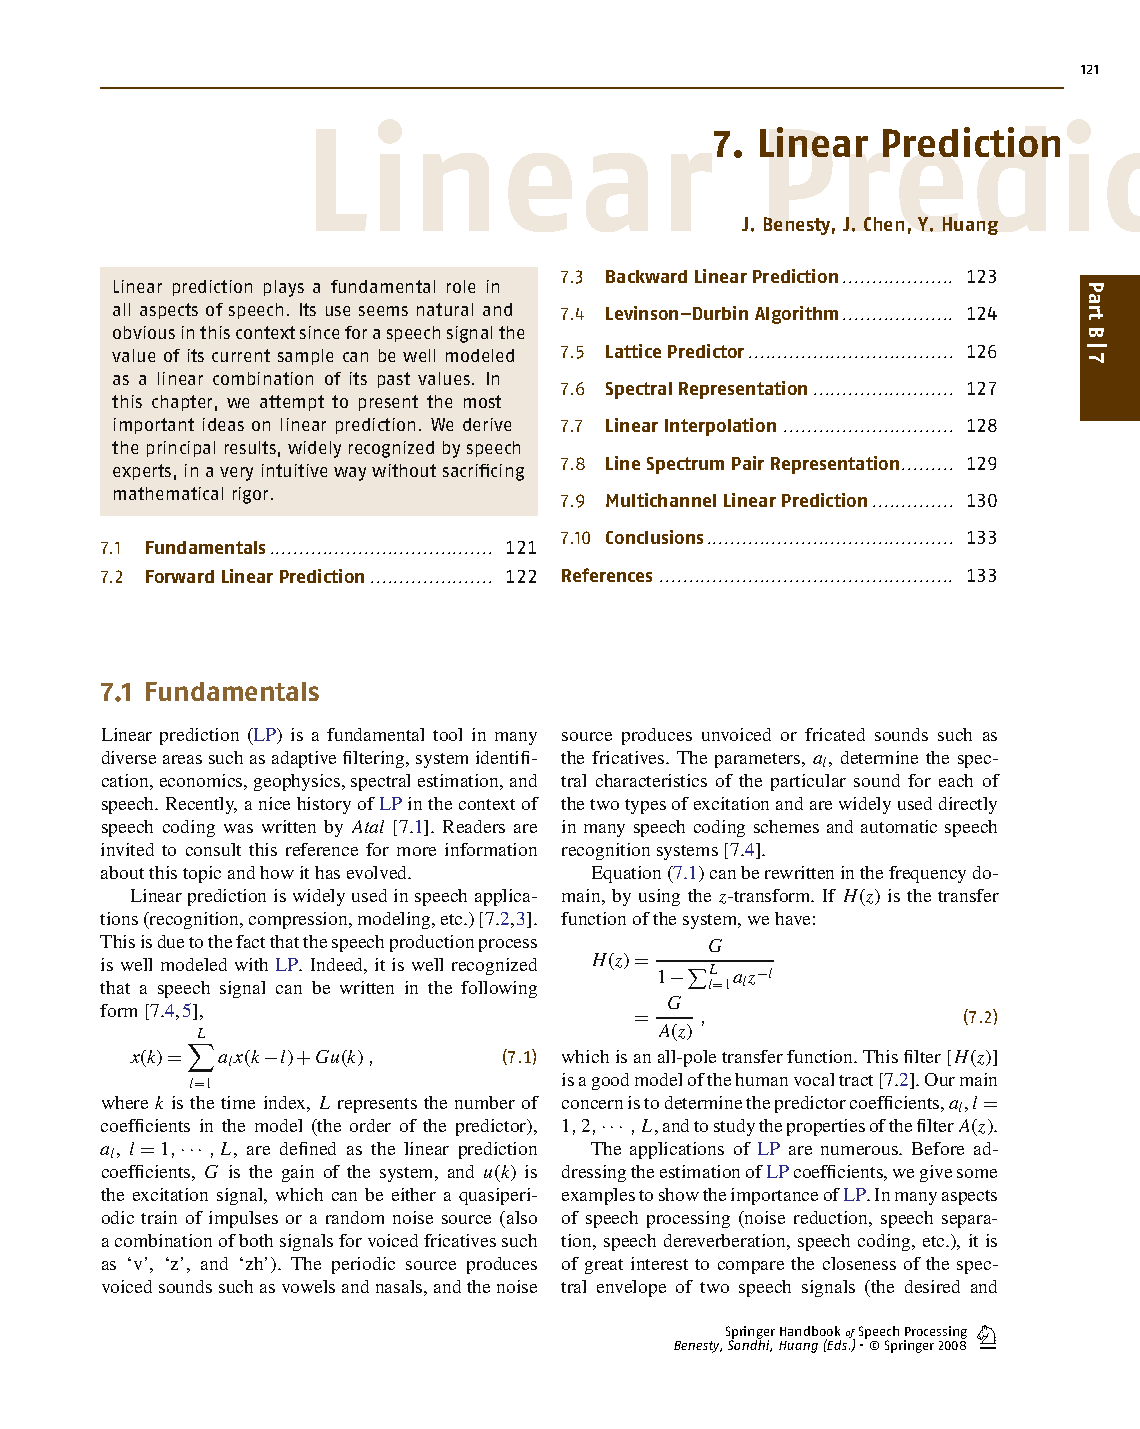
\includepdf[pages=-]{LinearPrediction}
\chapter{Transformée de Fourier rapide}
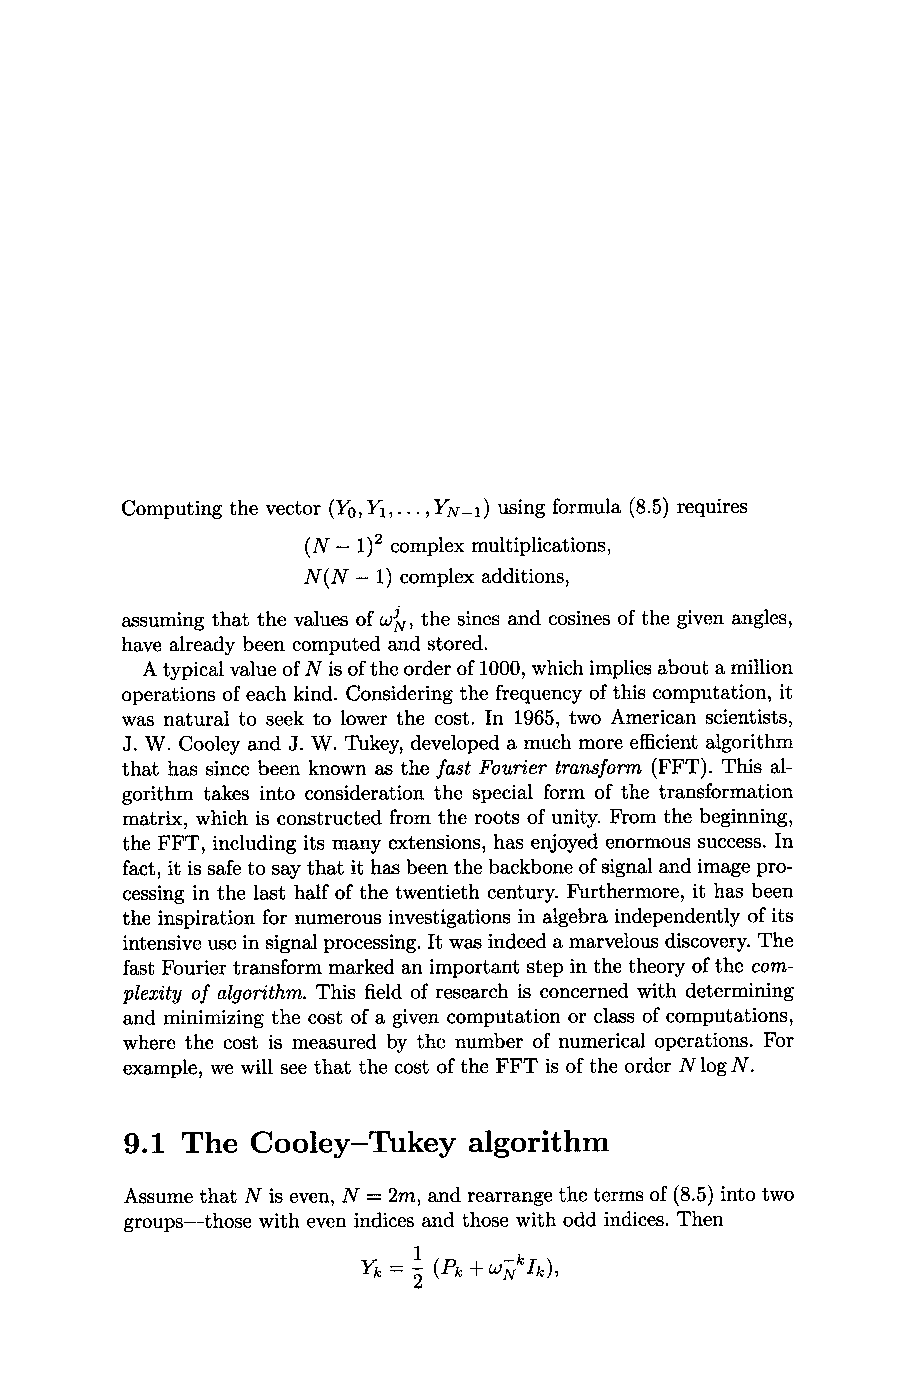
\includepdf[pages=-]{FFTgw}
\part{Documents}
\part{Production du signal de parole}
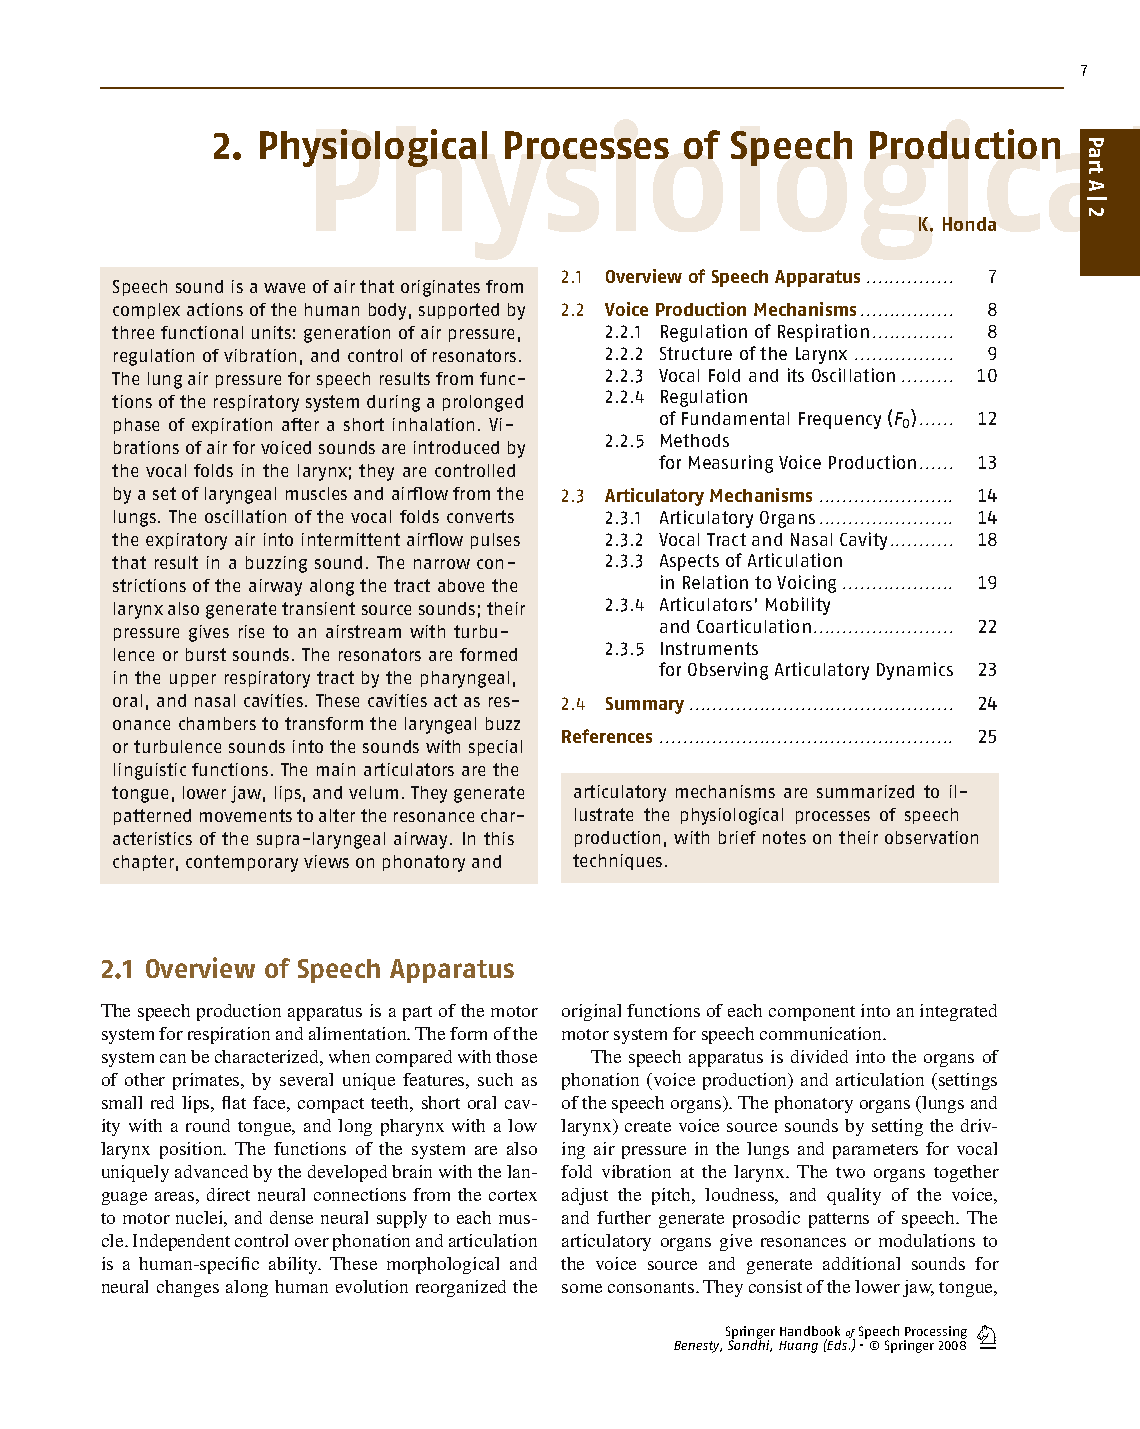
\includepdf[pages=-]{PhysiologicalProcessSpeech}
\end{document}
